\documentclass[]{book}
\usepackage{lmodern}
\usepackage{amssymb,amsmath}
\usepackage{ifxetex,ifluatex}
\usepackage{fixltx2e} % provides \textsubscript
\ifnum 0\ifxetex 1\fi\ifluatex 1\fi=0 % if pdftex
  \usepackage[T1]{fontenc}
  \usepackage[utf8]{inputenc}
\else % if luatex or xelatex
  \ifxetex
    \usepackage{mathspec}
  \else
    \usepackage{fontspec}
  \fi
  \defaultfontfeatures{Ligatures=TeX,Scale=MatchLowercase}
\fi
% use upquote if available, for straight quotes in verbatim environments
\IfFileExists{upquote.sty}{\usepackage{upquote}}{}
% use microtype if available
\IfFileExists{microtype.sty}{%
\usepackage{microtype}
\UseMicrotypeSet[protrusion]{basicmath} % disable protrusion for tt fonts
}{}
\usepackage[margin=1in]{geometry}
\usepackage{hyperref}
\hypersetup{unicode=true,
            pdftitle={Loss Data Analytics},
            pdfauthor={An open text authored by the Actuarial Community},
            pdfborder={0 0 0},
            breaklinks=true}
\urlstyle{same}  % don't use monospace font for urls
\usepackage{natbib}
\bibliographystyle{apalike}
\usepackage{color}
\usepackage{fancyvrb}
\newcommand{\VerbBar}{|}
\newcommand{\VERB}{\Verb[commandchars=\\\{\}]}
\DefineVerbatimEnvironment{Highlighting}{Verbatim}{commandchars=\\\{\}}
% Add ',fontsize=\small' for more characters per line
\usepackage{framed}
\definecolor{shadecolor}{RGB}{248,248,248}
\newenvironment{Shaded}{\begin{snugshade}}{\end{snugshade}}
\newcommand{\KeywordTok}[1]{\textcolor[rgb]{0.13,0.29,0.53}{\textbf{{#1}}}}
\newcommand{\DataTypeTok}[1]{\textcolor[rgb]{0.13,0.29,0.53}{{#1}}}
\newcommand{\DecValTok}[1]{\textcolor[rgb]{0.00,0.00,0.81}{{#1}}}
\newcommand{\BaseNTok}[1]{\textcolor[rgb]{0.00,0.00,0.81}{{#1}}}
\newcommand{\FloatTok}[1]{\textcolor[rgb]{0.00,0.00,0.81}{{#1}}}
\newcommand{\ConstantTok}[1]{\textcolor[rgb]{0.00,0.00,0.00}{{#1}}}
\newcommand{\CharTok}[1]{\textcolor[rgb]{0.31,0.60,0.02}{{#1}}}
\newcommand{\SpecialCharTok}[1]{\textcolor[rgb]{0.00,0.00,0.00}{{#1}}}
\newcommand{\StringTok}[1]{\textcolor[rgb]{0.31,0.60,0.02}{{#1}}}
\newcommand{\VerbatimStringTok}[1]{\textcolor[rgb]{0.31,0.60,0.02}{{#1}}}
\newcommand{\SpecialStringTok}[1]{\textcolor[rgb]{0.31,0.60,0.02}{{#1}}}
\newcommand{\ImportTok}[1]{{#1}}
\newcommand{\CommentTok}[1]{\textcolor[rgb]{0.56,0.35,0.01}{\textit{{#1}}}}
\newcommand{\DocumentationTok}[1]{\textcolor[rgb]{0.56,0.35,0.01}{\textbf{\textit{{#1}}}}}
\newcommand{\AnnotationTok}[1]{\textcolor[rgb]{0.56,0.35,0.01}{\textbf{\textit{{#1}}}}}
\newcommand{\CommentVarTok}[1]{\textcolor[rgb]{0.56,0.35,0.01}{\textbf{\textit{{#1}}}}}
\newcommand{\OtherTok}[1]{\textcolor[rgb]{0.56,0.35,0.01}{{#1}}}
\newcommand{\FunctionTok}[1]{\textcolor[rgb]{0.00,0.00,0.00}{{#1}}}
\newcommand{\VariableTok}[1]{\textcolor[rgb]{0.00,0.00,0.00}{{#1}}}
\newcommand{\ControlFlowTok}[1]{\textcolor[rgb]{0.13,0.29,0.53}{\textbf{{#1}}}}
\newcommand{\OperatorTok}[1]{\textcolor[rgb]{0.81,0.36,0.00}{\textbf{{#1}}}}
\newcommand{\BuiltInTok}[1]{{#1}}
\newcommand{\ExtensionTok}[1]{{#1}}
\newcommand{\PreprocessorTok}[1]{\textcolor[rgb]{0.56,0.35,0.01}{\textit{{#1}}}}
\newcommand{\AttributeTok}[1]{\textcolor[rgb]{0.77,0.63,0.00}{{#1}}}
\newcommand{\RegionMarkerTok}[1]{{#1}}
\newcommand{\InformationTok}[1]{\textcolor[rgb]{0.56,0.35,0.01}{\textbf{\textit{{#1}}}}}
\newcommand{\WarningTok}[1]{\textcolor[rgb]{0.56,0.35,0.01}{\textbf{\textit{{#1}}}}}
\newcommand{\AlertTok}[1]{\textcolor[rgb]{0.94,0.16,0.16}{{#1}}}
\newcommand{\ErrorTok}[1]{\textcolor[rgb]{0.64,0.00,0.00}{\textbf{{#1}}}}
\newcommand{\NormalTok}[1]{{#1}}
\usepackage{longtable,booktabs}
\usepackage{graphicx,grffile}
\makeatletter
\def\maxwidth{\ifdim\Gin@nat@width>\linewidth\linewidth\else\Gin@nat@width\fi}
\def\maxheight{\ifdim\Gin@nat@height>\textheight\textheight\else\Gin@nat@height\fi}
\makeatother
% Scale images if necessary, so that they will not overflow the page
% margins by default, and it is still possible to overwrite the defaults
% using explicit options in \includegraphics[width, height, ...]{}
\setkeys{Gin}{width=\maxwidth,height=\maxheight,keepaspectratio}
\IfFileExists{parskip.sty}{%
\usepackage{parskip}
}{% else
\setlength{\parindent}{0pt}
\setlength{\parskip}{6pt plus 2pt minus 1pt}
}
\setlength{\emergencystretch}{3em}  % prevent overfull lines
\providecommand{\tightlist}{%
  \setlength{\itemsep}{0pt}\setlength{\parskip}{0pt}}
\setcounter{secnumdepth}{5}
% Redefines (sub)paragraphs to behave more like sections
\ifx\paragraph\undefined\else
\let\oldparagraph\paragraph
\renewcommand{\paragraph}[1]{\oldparagraph{#1}\mbox{}}
\fi
\ifx\subparagraph\undefined\else
\let\oldsubparagraph\subparagraph
\renewcommand{\subparagraph}[1]{\oldsubparagraph{#1}\mbox{}}
\fi

%%% Use protect on footnotes to avoid problems with footnotes in titles
\let\rmarkdownfootnote\footnote%
\def\footnote{\protect\rmarkdownfootnote}

%%% Change title format to be more compact
\usepackage{titling}

% Create subtitle command for use in maketitle
\newcommand{\subtitle}[1]{
  \posttitle{
    \begin{center}\large#1\end{center}
    }
}

\setlength{\droptitle}{-2em}
  \title{Loss Data Analytics}
  \pretitle{\vspace{\droptitle}\centering\huge}
  \posttitle{\par}
  \author{An open text authored by the Actuarial Community}
  \preauthor{\centering\large\emph}
  \postauthor{\par}
  \predate{\centering\large\emph}
  \postdate{\par}
  \date{2017-11-12}

\usepackage{booktabs}
\setcounter{secnumdepth}{2}

\usepackage{amsthm}
\newtheorem{theorem}{Theorem}[chapter]
\newtheorem{lemma}{Lemma}[chapter]
\theoremstyle{definition}
\newtheorem{definition}{Definition}[chapter]
\newtheorem{corollary}{Corollary}[chapter]
\newtheorem{proposition}{Proposition}[chapter]
\theoremstyle{definition}
\newtheorem{example}{Example}[chapter]
\theoremstyle{definition}
\newtheorem{exercise}{Exercise}[chapter]
\theoremstyle{remark}
\newtheorem*{remark}{Remark}
\newtheorem*{solution}{Solution}
\begin{document}
\maketitle

{
\setcounter{tocdepth}{2}
\tableofcontents
}
\chapter*{Preface}\label{preface}
\addcontentsline{toc}{chapter}{Preface}

\subsubsection*{Book Description}\label{book-description}
\addcontentsline{toc}{subsubsection}{Book Description}

\textbf{Loss Data Analytics} is an interactive, online, freely available
text.

\begin{itemize}
\item
  The online version contains many interactive objects (quizzes,
  computer demonstrations, interactive graphs, video, and the like) to
  promote \emph{deeper learning}.
\item
  A subset of the book is available for \emph{offline reading} in pdf
  and EPUB formats.
\item
  The online text will be available in multiple languages to promote
  access to a \emph{worldwide audience}.
\end{itemize}

\subsubsection*{What will success look
like?}\label{what-will-success-look-like}
\addcontentsline{toc}{subsubsection}{What will success look like?}

The online text will be freely available to a worldwide audience. The
online version will contain many interactive objects (quizzes, computer
demonstrations, interactive graphs, video, and the like) to promote
deeper learning. Moreover, a subset of the book will be available in pdf
format for low-cost printing. The online text will be available in
multiple languages to promote access to a worldwide audience.

\subsubsection*{How will the text be
used?}\label{how-will-the-text-be-used}
\addcontentsline{toc}{subsubsection}{How will the text be used?}

This book will be useful in actuarial curricula worldwide. It will cover
the loss data learning objectives of the major actuarial organizations.
Thus, it will be suitable for classroom use at universities as well as
for use by independent learners seeking to pass professional actuarial
examinations. Moreover, the text will also be useful for the continuing
professional development of actuaries and other professionals in
insurance and related financial risk management industries.

\subsubsection*{Why is this good for the
profession?}\label{why-is-this-good-for-the-profession}
\addcontentsline{toc}{subsubsection}{Why is this good for the
profession?}

An online text is a type of open educational resource (OER). One
important benefit of an OER is that it equalizes access to knowledge,
thus permitting a broader community to learn about the actuarial
profession. Moreover, it has the capacity to engage viewers through
active learning that deepens the learning process, producing analysts
more capable of solid actuarial work. Why is this good for students and
teachers and others involved in the learning process?

Cost is often cited as an important factor for students and teachers in
textbook selection (see a recent post on the
\href{https://www.aei.org/publication/the-new-era-of-the-400-college-textbook-which-is-part-of-the-unsustainable-higher-education-bubble/}{\$400
textbook}). Students will also appreciate the ability to ``carry the
book around'' on their mobile devices.

\subsubsection*{Why loss data analytics?}\label{why-loss-data-analytics}
\addcontentsline{toc}{subsubsection}{Why loss data analytics?}

Although the intent is that this type of resource will eventually
permeate throughout the actuarial curriculum, one has to start
somewhere. Given the dramatic changes in the way that actuaries treat
data, loss data seems like a natural place to start. The idea behind the
name \emph{loss data analytics} is to integrate classical loss data
models from applied probability with modern analytic tools. In
particular, we seek to recognize that big data (including social media
and usage based insurance) are here and high speed computation s readily
available.

\subsubsection*{Project Goal}\label{project-goal}
\addcontentsline{toc}{subsubsection}{Project Goal}

The project goal is to have the actuarial community author our textbooks
in a collaborative fashion.

To get involved, please visit our
\href{https://sites.google.com/a/wisc.edu/loss-data-analytics/}{Loss
Data Analytics Project Site}.

\chapter{Introduction to Loss Data
Analytics}\label{introduction-to-loss-data-analytics}

\emph{Chapter Preview}. This book introduces readers to methods of
analyzing insurance data. Section 1 begins with a discussion of why the
use of data is important in the insurance industry. Yes, this is obvious
but we need to make a strong case for it as this is the whole premise of
the book. Next, Section 2 provides an overview of the types of data that
one encounters. There are many types from which to choose; your first
step in the analysis of data is identify a broad class to help direct
you to the appropriate tools and techniques. Section 3 gives a general
overview of the purposes of analyzing insurance data which is reinforced
in the Section 4 case study. Naturally, there is a huge gap between
identifying the broad class of variables and what we learn from the
data; this gap is covered through the methods and techniques of data
analysis covered in the rest of the text.

\section{Relevance of Analytics}\label{S:Intro}

In this section, you learn how to:

\begin{itemize}
\tightlist
\item
  Motivate the relevance of insurance
\item
  Describe analytics
\item
  Describe data generating events associated with the timeline of a
  typical insurance contract
\end{itemize}

This book introduces the process of using data to make decisions in an
insurance context. It does not assume that readers are familiar with
insurance but introduces insurance concepts as needed. Insurance may not
be as entertaining as the sports industry nor as widely familiar as the
agricultural industry but it does affect the financial livelihoods of
many. By almost any measure, insurance is a major economy activity. On a
global level, insurance premiums comprised about 6.3\% of the world
gross domestic product (GDP) in 2013, \citep{III2015}. To illustrate,
premiums accounted for 17.6\% of GDP in Taiwan (the highest in the
study) and represented 7.5\% of GDP in the United States. On a personal
level, almost everyone owning a home has insurance to protect themselves
in the event of a fire, hailstorm, or some other calamitous event.
Almost every country requires insurance for those driving a car. So,
although not particulary entertaining nor widely familiar, insurance is
an important piece of the economy and relevant to individual
livelihoods.

Insurance is a data-driven industry. Like other major corporations,
insurers use data when trying to decide how much to pay employees, how
many employees to retain, how to market their services, how to forecast
financial trends, and so on. Although each industry retains its own
nuances, these represent general areas of activities that are not
specific to the insurance industry. You will find that the data methods
and tools introduced in this text relevant for these general areas.

Moreover, when introducing data methods, we will focus on losses that
potentially arise from obligations in insurance contracts. This could be
the amount of damage to one's apartment under a renter's insurance
agreement, the amount needed to compensate someone that you hurt in a
driving accident, and the like. We will call these \emph{insurance
claims} or \emph{loss amounts}. With this focus, we will be able to
introduce generally applicable statistical tools in techniques in
real-life situations where the tools can be used directly.

\subsection{What is Analytics?}\label{what-is-analytics}

Insurance is a data-driven industry and analytics is a key to deriving
information from data. But what is analytics? Making data-driven
business decisions has been described as business analytics, business
intelligence, and data science. These terms, among others, are sometimes
used interchangeably and sometimes used separately, referring to
distinct domains of applications. As an example of such distinctions,
\emph{business intelligence} may focus on processes of collecting data,
often through databases and data warehouses, whereas \emph{business
analytics} utilizes tools and methods for statistical analyses of data.
In contrast to these two terms that emphasize business applications, the
term \emph{data science} can encompass broader applications in many
scientific domains. For our purposes, we use the term \emph{analytics}
to refer to the process of using data to make decisions. This process
involves gathering data, understanding models of uncertainty, making
general inferences, and communicating results.

\subsection{Short-term Insurance}\label{short-term-insurance}

This text will focus on short-term insurance contracts. By short-term,
we mean contracts where the insurance coverage is typically provided for
six months or a year. If you are new to insurance, then it is probably
easiest to think about an insurance policy that covers the contents of
an apartment or house that you are renting (known as renters insurance)
or the contents and property of a building that is owned by you or a
friend (known as homeowners insurance). Another easy example is
automobile insurance. In the event of an accident, this policy may cover
damage to your vehicle, damage to other vehicles in the accident, as
well as medical expenses of those injured in the accident.

In the US, policies such as renters and homeowners are known as property
insurance whereas a policy such as auto that covers medical damages to
people is known as casualty insurance. In the rest of the world, these
are both known as nonlife or general insurance, to distinguish them from
life insurance.

Both life and nonlife insurances are important. To illustrate,
\citep{III2015} estimates that direct insurance premiums in the world
for 2013 was 2,608,091 for life and 2,032,850 for nonlife; these figures
are in millions of US dollars. As noted earlier, the total represents
6.3\% of the world GDP. Put another way, life accounts for 56.2\% of
insurance premiums and 3.5\% of world GDP, nonlife accounts for 43.8\%
of insurance premiums and 2.7\% of world GDP. Both life and nonlife
represent important economic activities and are worthy of study in their
own right.

Yet, life insurance considerations differ from nonlife. In life
insurance, the default is to have a multi-year contract. For example, if
a person 25 years old purchases a whole life policy that pays upon death
of the insured and that person does not die until age 100, then the
contract is in force for 75 years. We think of this as a long-term
contract.

Further, in life insurance, the benefit amount is often stipulated in
the contract provisions. In contrast, most short-term contracts provide
for reimbursement of insured losses which are unknown before the
accident. (Of course, there are usually limits placed on the
reimbursement amounts.) In a multi-year life insurance contract, the
time value of money plays a prominent role. In contrast, in a short-term
nonlife contract, the random amount of reimbursement takes priority.

In both life and nonlife insurances, the frequency of claims is very
important. For many life insurance contracts, the insured event (such as
death) happens only once. In contrast, for nonlife insurances such as
automobile, it is common for individuals (especially young male drivers)
to get into more than one accident during a year. So, our models need to
reflect this observation; we will introduce different frequency models
than you may have seen when studying life insurance.

For short-term insurance, the framework of the probabilistic model is
straightforward. We think of a one-period model (the period length,
e.g., six months, will be specified in the situation).

\begin{itemize}
\item
  At the beginning of the period, the insured pays the insurer a known
  premium that is agreed upon by both parties to the contract.
\item
  At the end of the period, the insurer reimburses the insured for a
  (possibly multivariate) random loss that we will denote as \(y\).
\end{itemize}

This framework will be developed as we proceed but we first focus on
integrating this framework with concerns about how the data may arise
and what we can accomplish with this framework.

\subsection{Insurance Processes}\label{S:InsProcesses}

One way to describe the data arising from operations of a company that
sells insurance products is to adopt a granular approach. In this micro
oriented view, we can think specifically about what happens to a
contract at various stages of its existence. Consider Figure
\ref{fig:StochOperations} that traces a timeline of a typical insurance
contract. Throughout the existence of the contract, the company
regularly processes events such as premium collection and valuation,
described in Section \ref{S:PredModApps}; these are marked with an
\textbf{x} on the timeline. Further, non-regular and unanticipated
events also occur. To illustrate, times \(\mathrm{t}_2\) and
\(\mathrm{t}_4\) mark the event of an insurance claim (some contracts,
such as life insurance, can have only a single claim). Times
\(\mathrm{t}_3\) and \(\mathrm{t}_5\) mark the events when a
policyholder wishes to alter certain contract features, such as the
choice of a deductible or the amount of coverage. Moreover, from a
company perspective, one can even think about the contract initiation
(arrival, time \(\mathrm{t}_1\)) and contract termination (departure,
time \(\mathrm{t}_6\)) as uncertain events.





\begin{figure}

{\centering 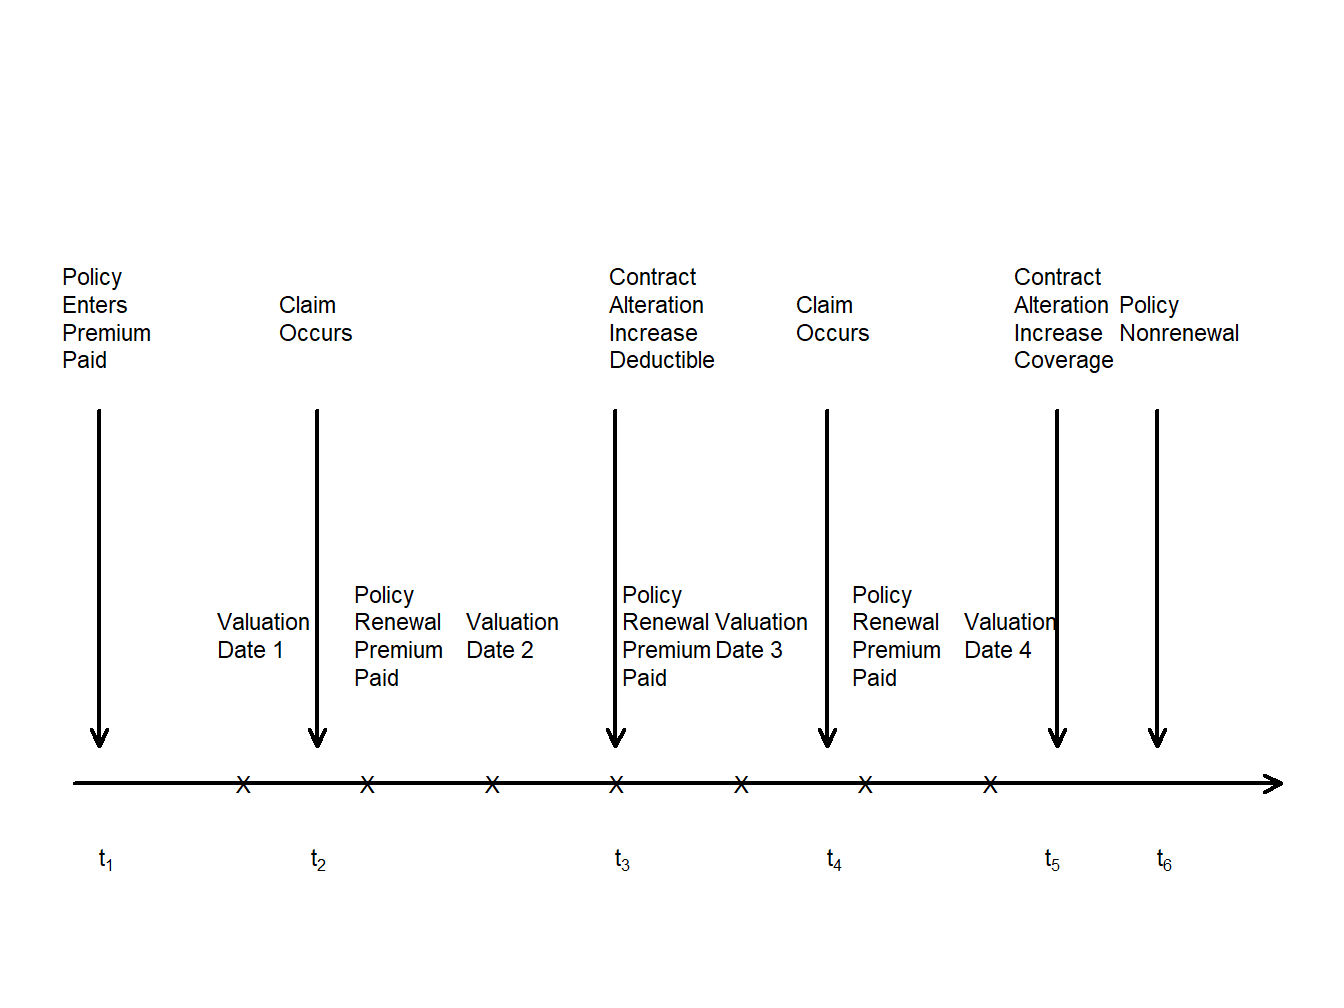
\includegraphics[width=1\linewidth]{LossDataAnalytics_files/figure-latex/StochOperations-1} 

}

\caption{Timeline of a Typical Insurance Policy. Arrows
mark the occurrences of random events. Each x marks the time of
scheduled events that are typically non-random.}\label{fig:StochOperations}
\end{figure}

\section{Variable Types}\label{variable-types}

In this section, you learn how to:

\begin{itemize}
\tightlist
\item
  Describe different types of variables typically encountered in
  insurance practice
\item
  Classify a variable into the appropriate category
\end{itemize}

Before discussing how to use insurance data to make decisions, it is
helpful to first describe common features of data. In general, people,
firms, and other entities that we want to understand are described in a
dataset by numerical characteristics. As these characteristics vary by
entity, they are commonly known as \emph{variables}. To manage insurance
systems, it will be critical to understand the distribution of each
variable and how they are associated with one another. We will encounter
datasets that have many variables (high dimensional) and so it useful to
begin by classifying them into different types. As will be seen, this
classification is not strict; there is overlap among the types.
Nonetheless, the classification summarized in Table \ref{tab:VarTypes}
and explained in the remainder of this section provide a solid first
step in framing a dataset.

Table: \label{tab:VarTypes} Variable Types

\[{\small \begin{matrix}
\begin{array}{l|l} \hline
\textbf{Variable Type} & \textbf{Example} \\\hline
Qualitative &            \\
    \text{Binary} &        \text{Sex} \\
\text{Categorical (Unordered, Nominal)} & \text{Territory (e.g., state/province) in which an insured resides} \\
\text{Ordered Category (Ordinal)} & \text{Claimant satisfaction (five point scale ranging from 1=dissatisfied} \\
& ~~~ \text{to 5 =satisfied)} \\\hline
Quantitative &            \\
\text{Continuous} & \text{Policyholder's age, weight, income} \\
  \text{Discrete} & \text{Amount of deductible} \\
\text{Count} & \text{Number of insurance claims} \\
\text{Combinations of}  & \text{Policy losses, mixture of 0's (for no loss)}  \\
~~~ \text{Discrete and Continuous} & ~~~\text{and positive claim amount} \\
\text{Interval Variable} & \text{Driver Age: 16-24 (young), 25-54 (intermediate),}  \\
& ~~~\text{55 and over (senior)} \\
\text{Circular Data} & \text{Time of day measures of customer arrival} \\ \hline
Multivariate ~ Variable &            \\
\text{High Dimensional Data} & \text{Characteristics of a firm purchasing worker's compensation} \\
& ~~~\text{insurance (location of plants, industry, number of employees,} \\
&~~~\text{and so on)} \\
\text{Spatial Data} & \text{Longitude/latitude of the location an insurance hailstorm claim} \\
\text{Missing Data} & \text{Policyholder's age (continuous/interval) and "-99" for} \\
&~~~ \text{"not reported," that is, missing} \\
\text{Censored and Truncated Data} & \text{Amount of insurance claims in excess of a deductible} \\
\text{Aggregate Claims} & \text{Losses recorded for each claim in a motor vehicle policy.} \\
\text{Stochastic Process Realizations} & \text{The time and amount of each occurrence of an insured loss} \\ \hline
\end{array}
\end{matrix}}
\]

\subsection{Qualitative Variables}\label{qualitative-variables}

Let us start with the simplest type, a binary variable. As suggested by
its name, a \emph{binary variable} is one with only two possible values.
Although not necessary, the two values are commonly taken to be a 0 and
a 1. Binary variables are typically used to indicate whether or not an
entity possesses an attribute. For example, we might code a variable in
a dataset to be a 1 if an insured is female and a 0 if male. (An
\emph{insured} is a person who is covered under an insurance agreement.)

More generally, a \emph{qualitative}, or \emph{categorical}, variable is
one for which the measurement denotes membership in a set of groups, or
categories. For example, if you were coding in which area of the country
in which an insured resides, you might use a 1 for the northern part, 2
for southern, and 3 for everything else. A binary variable is a special
type of categorical variable where there are only two categories. This
location variable is an example of a \emph{nominal} variable, one for
which the levels have no natural ordering. Any analysis of nominal
variables should not depend on the labeling of the categories. For
example, instead of using a 1,2,3 for north, south, other, I should
arrive at the same set of summary statistics if I used a 2,1,3 coding
instead, interchanging north and south.

In contrast, an \emph{ordinal} variable is a type of categorical
variable for which an ordering does exist. For example, with a survey to
see how satisfied customers are with our claims servicing department, we
might use a five point scale that ranges from 1 meaning dissatisfied to
a 5 meaning satisfied. Ordinal variables provide a clear ordering of
levels of a variable but the amount of separation between levels is
unknown.

\subsection{Quantitative Variables}\label{quantitative-variables}

Unlike a qualitative variable, a quantitative variable is one in which
numerical level is a realization from some scale so that the distance
between any two levels of the scale takes on meaning.

A \emph{continuous variable} is one that can take on any value within a
finite interval. For example, it is common to represent a policyholder's
age, weight, or income, as a continuous variable.

In contrast, a \emph{discrete variable} is one that takes on only a
finite number of values in any finite interval. For example, when
examining a policyholder's choice of deductibles, it may be that values
of 0, 250, 500, and 1000 are the only possible outcomes. Like a ordinal
variable, these represent distinct categories that are ordered. Unlike
an ordinal variable, the numerical difference between levels takes on
economic meaning.

A special type of discrete variable is a \emph{count variable}, one with
values on the nonnegative integers \(0, 1, 2, \ldots.\) For example, we
will be particularly interested in the number of claims arising from a
policy during a given period. This is known as the \emph{claim
frequency}.

Given that we will develop ways to analyze discrete variables, do we
really need separate methods for dealing with continuous variables?
After all, one can argue that few things in the physical world are truly
continuous. For example, each currency has a smallest unit that is not
subdivided further. (In the US, you cannot pay for anything smaller than
one cent.) Nonetheless, models using continuous variables serve as
excellent approximations to real-world discrete outcomes, in part due to
their simplicity. It will be well worth our time and effort to develop
models and analyze continuous and discrete variables differently.

Having said that, some variables are inherently a \emph{combination of
discrete and continuous} components. For example, when we analyze the
insured loss of a policyholder, we will encounter a discrete outcome at
zero, representing no insured loss, and a continuous amount for positive
outcomes, representing the amount of the insured loss.

Another interesting variation is an \emph{interval variable}, one that
gives a range of possible outcomes. For example, instead of recording a
driver's age in year, it is common for insurers to group ages into three
categories, (i) ages 16-24, representing young drives, (ii) ages 25-54,
representing intermediate age drivers, and (iii) ages 55 and over,
representing senior drivers.

\emph{Circular data} represent an interesting category typically not
analyzed by insurers. As an example of circular data, suppose that you
monitor calls to your customer service center and would like to know
when is the peak time of the day for calls to arrive. In this context,
one can think about the time of the day as a variable with realizations
on a circle, e.g., imagine an analog picture of a clock. For circular
data, the distance between observations at 00:15 and 00:45 are just as
close as observations 23:45 and 00:15 (here, we use the convention
\emph{HH:MM} means hours and minutes).

\subsection{Multivariate Variables}\label{multivariate-variables}

Insurance data are typically are \emph{multivariate} in the sense that
we can take many measurements on a single entity. For example, when
studying losses associated with a firm's worker's compensation plan, we
might want to know the location of its manufacturing plants, the
industry in which it operates, the number of employees, and so forth. If
there are many variables, such data are also known as \emph{high
dimensional}.

The usual strategy for analyzing multivariate data is to begin by
examining each variable in isolation of the others. This is known as a
\emph{univariate} approach. By considering only one measurement,
variables are \emph{scalars} and, as described, can be thought broadly
as either qualitative or quantitative.

In contrast, for some variables, it makes little sense to only look a
one dimensional aspects. For example, insurers typically organize
\emph{spatial} data by longitude and latitude to analyze the location of
weather related insurance claims due hailstorms. Having only a single
number, either longitude or latitude, provides little information in
understanding geographical location.

Another special case of a multivariate variable, less obvious, involves
coding for \emph{missing data}. Historically, some statistical packages
used a -99 to report when a variable, such as policyholder's age, was
not available or not reported. This led to many unsuspecting analysts
providing strange statistics when summarizing a set of data. When data
are missing, it is better to think about the variable as two dimensions,
one to indicate whether or not the variable is reported and the second
providing the age (if reported).

In the same way, insurance data are commonly \emph{censored} and
\emph{truncated}. To illustrate, with automobile claims may be limited
or censored by 500,000, the upper limit that the insurer will pay. The
loss amount may be in excess of 500000 but the insurer is only aware of
its payout. To record censored claims, a binary variable is used to
indicate whether or not the claim is censored (limited) and a second
variable is used to indicate the payout. In the same way, claims may be
truncated by a deductible. Although there are many types of deductibles,
in a common form the insurer pays the amount in excess of a deductible.
To illustrate, suppose you have an auto policy with a 250 deductible. If
you have a 1000 loss, then the insurer pays 750. If you have a 200 loss,
then the insurer pays nothing. In principle, one would like to use a
binary variable to indicate whether or not the claim has a deductible
and a second variable is used to indicate the payout. As we will see,
the tricky thing about deductibles is that for many sampling schemes,
the insurer does not observe a claim if it the loss falls below the
deductible amount. More on this topic later.

\emph{Aggregate claims} can also be coded as another special type of
multivariate variable. In this situation, an insurer has potentially
zero, one, two, or more claims, within a policy period. Each claim has
its own level (possibly mediated by deductibles and upper limits) and
there are an uncertain, or random, number of each claims for each
individual. This is a case where the the dimension of the multivariate
variable is not known in advance.

Perhaps the most complicated type of multivariate variable is a
\emph{realization of a stochastic process}. You will recall that a
stochastic process is little more than a collection of random variables.
For example, in insurance, we might think about the times that claims
arrive to an insurance company in a one year time horizon. This is a
high dimensional variable that theoretically is infinite dimensional.
Special techniques are required to understand realizations of stochastic
processes that will not be addressed here.

\section{Insurance Company Operations}\label{S:PredModApps}

In this section, you learn how to:

\begin{itemize}
\tightlist
\item
  Describe five major operational areas of insurance companies.
\item
  Identify the role of data and analytics opportunities within each
  operational area.
\end{itemize}

Armed with insurance data and a method of organizing the data into
variable types, the end goal is to use data to make decisions. Of
course, we will need to learn more about methods of analyzing and
extrapolating data but that is the purpose of the remaining chapters in
the text. To begin, let us think about why we wish to do the analysis.
To provide motivation, we take the insurer's viewpoint (not a person)
and introduce ways of bringing money in, paying it out, managing costs,
and making sure that we have enough money to meet obligations.

Specifically, in many insurance companies, it is customary to aggregate
detailed insurance processes into larger operational units; many
companies use these functional areas to segregate employee activities
and areas of responsibilities. Actuaries and other financial analysts
work within these units and use data for the following activities:

\begin{enumerate}
\def\labelenumi{\arabic{enumi}.}
\item
  \textbf{Initiating Insurance}. At this stage, the company makes a
  decision as to whether or not to take on a risk (the
  \emph{underwriting} stage) and assign an appropriate premium (or
  rate). Insurance analytics has its actuarial roots in
  \emph{ratemaking}, where analysts seek to determine the right price
  for the right risk.
\item
  \textbf{Renewing Insurance}. Many contracts, particularly in general
  insurance, have relatively short durations such as 6 months or a year.
  Although there is an implicit expectation that such contracts will be
  renewed, the insurer has the opportunity to decline coverage and to
  adjust the premium. Analytics is also used at this policy renewal
  stage where the goal is to retain profitable customers.
\item
  \textbf{Claims Management}. Analytics has long been used in (1)
  detecting and preventing claims fraud, (2) managing claim costs,
  including identifying the appropriate support for claims handling
  expenses, as well as (3) understanding excess layers for reinsurance
  and retention.
\item
  \textbf{Loss Reserving}. Analytic tools are used to provide management
  with an appropriate estimate of future obligations and to quantify the
  uncertainty of the estimates.
\item
  \textbf{Solvency and Capital Allocation}. Deciding on the requisite
  amount of capital and ways of allocating capital to alternative
  investment activities represent other important analytics activities.
  Companies must understand how much capital is needed so that they will
  have sufficient flow of cash available to meet their obligations. This
  is an important question that concerns not only company managers but
  also customers, company shareholders, regulatory authorities, as well
  as the public at large. Related to issues of how much capital is the
  question of how to allocate capital to differing financial projects,
  typically to maximize an investor's return. Although this question can
  arise at several levels, insurance companies are typically concerned
  with how to allocate capital to different lines of business within a
  firm and to different subsidiaries of a parent firm.
\end{enumerate}

Although data is a critical component of solvency and capital
allocation, other components including an economic framework and
financial investments environment are also important. Because of the
background needed to address these components, we will not address
solvency and capital allocation issues further in this text.

Nonetheless, for all operating functions, we emphasize that analytics in
the insurance industry is not an exercise that a small group of analysts
can do by themselves. It requires an insurer to make significant
investments in their information technology, marketing, underwriting,
and actuarial functions. As these areas represent the primary end goals
of the analysis of data, additional background on each operational unit
is provided in the following subsections.

\subsection{Initiating Insurance}\label{initiating-insurance}

Setting the price of an insurance good can be a perplexing problem. In
manufacturing, the cost of a good is (relatively) known and provides a
benchmark for assessing a market demand price. In other areas of
financial services, market prices are available and provide the basis
for a market-consistent pricing structure of products. In contrast, for
many lines of insurance, the cost of a good is uncertain and market
prices are unavailable. Expectations of the random cost is a reasonable
place to start for a price, as this is the optimal price for a
risk-neutral insurer. Thus, it has been traditional in insurance pricing
to begin with the expected cost and to add to this so-called margins to
account for the product's riskiness, expenses incurred in servicing the
product, and a profit/surplus allowance for the insurance company.

For some lines of business, especially automobile and homeowners
insurance, analytics has served to sharpen the market by making the
calculation of the good's expectation more precise. The increasing
availability of the internet among consumers has promoted transparency
in pricing. Insurers seek to increase their market share by refining
their risk classification systems and employing skimming the cream
underwriting strategies. Recent surveys (e.g., \citep{survey2013})
indicate that pricing is the most common use of analytics among
insurers.

\emph{Underwriting}, the process of classifying risks into homogenous
categories and assigning policyholders to these categories, lies at the
core of ratemaking. Policyholders within a class have similar risk
profiles and so are charged the same insurance price. This is the
concept of an actuarially fair premium; it is fair to charge different
rates to policyholders only if they can be separated by identifiable
risk factors. To illustrate, an early contribution, Two Studies in
Automobile Insurance Ratemaking, by \citep{bailey1960} provided a
catalyst to the acceptance of analytic methods in the insurance
industry. This paper addresses the problem of classification ratemaking.
It describes an example of automobile insurance that has five use
classes cross-classified with four merit rating classes. At that time,
the contribution to premiums for use and merit rating classes were
determined independently of each other. Thinking about the interacting
effects of different classification variables is a more difficult
problem.

\subsection{Renewing Insurance}\label{renewing-insurance}

Insurance is a type of financial service and, like many service
contracts, insurance coverage is often agreed upon for a limited time
period, such as six months or a year, at which time commitments are
complete. Particularly for general insurance, the need for coverage
continues and so efforts are made to issue a new contract providing
similar coverage. Renewal issues can also arise in life insurance, e.g.,
term (temporary) life insurance, although other contracts, such as life
annuities, terminate upon the insured's death and so issues of
renewability are irrelevant.

In absence of legal restrictions, at renewal the insurer has the
opportunity to:

\begin{itemize}
\item
  accept or decline to underwrite the risk and
\item
  determine a new premium, possibly in conjunction with a new
  classification of the risk.
\end{itemize}

Risk classification and rating at renewal is based on two types of
information. First, as at the initial stage, the insurer has available
many rating variables upon which decisions can be made. Many variables
will not change, e.g., sex, whereas others are likely to have changed,
e.g., age, and still others may or may not change, e.g., credit score.
Second, unlike the initial stage, at renewal the insurer has available a
history of policyholder's loss experience, and this history can provide
insights into the policyholder that are not available from rating
variables. Modifying premiums with claims history is known as
\emph{experience rating}, also sometimes referred to as \emph{merit
rating}.

Experience rating methods are either applied retrospectively or
prospectively. With retrospective methods, a refund of a portion of the
premium is provided to the policyholder in the event of favorable (to
the insurer) experience. Retrospective premiums are common in life
insurance arrangements (where policyholders earned dividends in the U.S.
and bonuses in the U.K.). In general insurance, prospective methods are
more common, where favorable insured experience is rewarded through a
lower renewal premium.

Claims history can provide information about a policyholder's risk
appetite. For example, in personal lines it is common to use a variable
to indicate whether or not a claim has occurred in the last three years.
As another example, in a commercial line such as worker's compensation,
one may look to a policyholder's average claim over the last three
years. Claims history can reveal information that is hidden (to the
insurer) about the policyholder.

\subsection{Claims and Product
Management}\label{claims-and-product-management}

In some of areas of insurance, the process of paying claims for insured
events is relatively straightforward. For example, in life insurance, a
simple death certificate is all that is needed as the benefit amount is
provided in the contract terms. However, in non-life areas such as
property and casualty insurance, the process is much more complex. Think
about even a relatively simple insured event such as automobile
accident. Here, it is often helpful to determine which party is at
fault, one needs to assess damage to all of the vehicles and people
involved in the incident, both insured and non-insured, the expenses
incurred in assessing the damages, and so forth. The process of
determining coverage, legal liability, and settling claims is known as
\emph{claims adjustment}.

Insurance managers sometimes use the phrase \emph{claims leakage} to
mean dollars lost through claims management inefficiencies. There are
many ways in which analytics can help manage the claims process,
\citep{SASsurvey}. Historically, the most important has been fraud
detection. The claim adjusting process involves reducing information
asymmetry (the claimant knows exactly what happened; the company knows
some of what happened). Mitigating fraud is an important part of claims
management process.

One can think about the management of claims severity as consisting of
the following components:

\begin{itemize}
\item
  \textbf{Claims triaging}. Just as in the medical world, early
  identification and appropriate handling of high cost claims (patients,
  in the medical world), can lead to dramatic company savings. For
  example, in workers compensation, insurers look to achieve early
  identification of those claims that run the risk of high medical costs
  and a long payout period. Early intervention into those cases could
  give insurers more control over the handling of the claim, the medical
  treatment, and the overall costs with an earlier return-to-work.
\item
  \textbf{Claims processing}. The goal is to use analytics to identify
  situations suitable for small claims handling processes and those for
  adjuster assignment to complex claims.
\item
  \textbf{Adjustment decisions}. Once a complex claim has been
  identified and assigned to an adjuster, analytic driven routines can
  be established to aid subsequent decision-making processes. Such
  processes can also be helpful for adjusters in developing case
  reserves, an important input to the insurer's loss reserves, Section
  \ref{S:Reserving}.
\end{itemize}

In addition to the insured's reimbursement for insured losses, the
insurer also needs to be concerned with another source of revenue
outflow, expenses. Loss adjustment expenses are part of an insurer's
cost of managing claims. Analytics can be used to reduce expenses
directly related to claims handling (allocated) as well as general staff
time for overseeing the claims processes (unallocated). The insurance
industry has high operating costs relative to other portions of the
financial services sectors.

In addition to claims payments, there are many other ways in which
insurers use to data to manage their products. We have already discussed
the need for analytics in underwriting, that is, risk classification at
the initial acquisition stage. Insurers are also interested in which
policyholders elect to renew their contract and, as with other products,
monitor customer loyalty.

Analytics can also be used to manage the portfolio, or collection, of
risks that an insurer has acquired. When the risk is initially obtained,
the insurer's risk can be managed by imposing contract parameters that
modify contract payouts. In Chapter xx introduces common modifications
including coinsurance, deductibles, and policy upper limits.

After the contract has been agreed upon with an insured, the insurer may
still modify its net obligation by entering into a reinsurance
agreement. This type of agreement is with a reinsurer, an insurer of an
insurer. It is common for insurance companies to purchase insurance on
its portfolio of risks to gain protection from unusual events, just as
people and other companies do.

\subsection{Loss Reserving}\label{S:Reserving}

An important feature that distinguishes insurance from other sectors of
the economy is the timing of the exchange of considerations. In
manufacturing, payments for goods are typically made at the time of a
transaction. In contrast, for insurance, money received from a customer
occurs in advance of benefits or services; these are rendered at a later
date. This leads to the need to hold a reservoir of wealth to meet
future obligations in respect to obligations made. The size of this
reservoir of wealth, and the importance of ensuring its adequacy in
regard to liabilities already assumed, is a major concern for the
insurance industry.

Setting aside money for unpaid claims is known as \emph{loss reserving};
in some jurisdictions, reserves are also known as \emph{technical
provisions}. We saw in Figure \ref{fig:StochOperations} how future
obligations arise naturally at a specific (valuation) date; a company
must estimate these outstanding liabilities when determining its
financial strength. Accurately determining loss reserves is important to
insurers for many reasons.

\begin{enumerate}
\def\labelenumi{\arabic{enumi}.}
\item
  Loss reserves represent a loan that the insurer owes its customers.
  Under-reserving may result in a failure to meet claim liabilities.
  Conversely, an insurer with excessive reserves may present a weaker
  financial position than it truly has and lose market share.
\item
  Reserves provide an estimate for the unpaid cost of insurance that can
  be used for pricing contracts.
\item
  Loss reserving is required by laws and regulations. The public has a
  strong interest in the financial strength of insurers.
\item
  In addition to the insurance company management and regulators, other
  stakeholders such as investors and customers make decisions that
  depend on company loss reserves.
\end{enumerate}

Loss reserving is a topic where there are substantive differences
between life and general (also known as property and casualty, or
non-life), insurance. In life insurance, the severity (amount of loss)
is often not a source of concern as payouts are specified in the
contract. The frequency, driven by mortality of the insured, is a
concern. However, because of the length of time for settlement of life
insurance contracts, the time value of money uncertainty as measured
from issue to date of death can dominate frequency concerns. For
example, for an insured who purchases a life contract at age 20, it
would not be unusual for the contract to still be open in 60 years time.
See, for example, \citep{bowers1986actuarial} or
\citep{dickson2013actuarial} for introductions to reserving for life
insurance.

\section{Case Study: Wisconsin Property Fund}\label{S:LGPIF}

In this section,for a real case study such as the Wisconsin Property
Fund, you learn how to:

\begin{itemize}
\tightlist
\item
  Describe how data generating events can produce data of interest to
  insurance analysts.
\item
  Identify the type of each variable.
\item
  Produce relevant summary statistics for each variable.
\item
  Describe how these summary statistcs can be used in each of the major
  operational areas of an insurance company.
\end{itemize}

Let us illustrate the kind of data under consideration and the goals
that we wish to achieve by examining the Local Government Property
Insurance Fund (LGPIF), an insurance pool administered by the Wisconsin
Office of the Insurance Commissioner. The LGPIF was established to
provide property insurance for local government entities that include
counties, cities, towns, villages, school districts, and library boards.
The fund insures local government property such as government buildings,
schools, libraries, and motor vehicles. The fund covers all property
losses except those resulting from flood, earthquake, wear and tear,
extremes in temperature, mold, war, nuclear reactions, and embezzlement
or theft by an employee.

The property fund covers over a thousand local government entities who
pay approximately \$25 million in premiums each year and receive
insurance coverage of about \$75 billion. State government buildings are
not covered; the LGPIF is for local government entities that have
separate budgetary responsibilities and who need insurance to moderate
the budget effects of uncertain insurable events. Coverage for local
government property has been made available by the State of Wisconsin
since 1911.

\subsection{Fund Claims Variables}\label{S:OutComes}

At a fundamental level, insurance companies accept premiums in exchange
for promises to indemnify a policyholder upon the uncertain occurrence
of an insured event. This indemnification is known as a \emph{claim}. A
positive amount, also known as the \emph{severity} of the claim, is a
key financial expenditure for an insurer. So, knowing only the claim
amount summarizes the reimbursement to the policyholder.

Ignoring expenses, an insurer that examines only amounts paid would be
indifferent to two claims of 100 when compared to one claim of 200, even
though the number of claims differ. Nonetheless, it is common for
insurers to study how often claims arise, known as the \emph{frequency}
of claims. The frequency is important for expenses, but it also
influences contractual parameters (such as deductibles and policy
limits) that are written on a per occurrence basis, is routinely
monitored by insurance regulators, and is often a key driven in the
overall indemnification obligation of the insurer. We shall consider the
two claims variables, the severity and frequency, as the two main
outcome variables that we wish to understand, model, and manage.

To illustrate, in 2010 there were 1,110 policyholders in the property
fund. Table \ref{tab:Frequency2010} shows the distribution of the 1,377
claims. Almost two-thirds (0.637) of the policyholders did not have any
claims and an additional 18.8\% only had one claim. The remaining 17.5\%
(=1 - 0.637 - 0.188) had more than one claim; the policyholder with the
highest number recorded 239 claims. The average number of claims for
this sample was 1.24 (=1377/1110).

\begin{longtable}[]{@{}llllllllllll@{}}
\caption{\label{tab:Frequency2010} 2010 Claims Frequency
Distribution}\tabularnewline
\toprule
\begin{minipage}[b]{0.08\columnwidth}\raggedright\strut
Type\strut
\end{minipage} & \begin{minipage}[b]{0.08\columnwidth}\raggedright\strut
\strut
\end{minipage} & \begin{minipage}[b]{0.08\columnwidth}\raggedright\strut
\strut
\end{minipage} & \begin{minipage}[b]{0.08\columnwidth}\raggedright\strut
\strut
\end{minipage} & \begin{minipage}[b]{0.08\columnwidth}\raggedright\strut
\strut
\end{minipage} & \begin{minipage}[b]{0.08\columnwidth}\raggedright\strut
\strut
\end{minipage} & \begin{minipage}[b]{0.08\columnwidth}\raggedright\strut
\strut
\end{minipage} & \begin{minipage}[b]{0.08\columnwidth}\raggedright\strut
\strut
\end{minipage} & \begin{minipage}[b]{0.08\columnwidth}\raggedright\strut
\strut
\end{minipage} & \begin{minipage}[b]{0.08\columnwidth}\raggedright\strut
\strut
\end{minipage} & \begin{minipage}[b]{0.08\columnwidth}\raggedright\strut
\strut
\end{minipage} & \begin{minipage}[b]{0.08\columnwidth}\raggedright\strut
\strut
\end{minipage}\tabularnewline
\midrule
\endfirsthead
\toprule
\begin{minipage}[b]{0.08\columnwidth}\raggedright\strut
Type\strut
\end{minipage} & \begin{minipage}[b]{0.08\columnwidth}\raggedright\strut
\strut
\end{minipage} & \begin{minipage}[b]{0.08\columnwidth}\raggedright\strut
\strut
\end{minipage} & \begin{minipage}[b]{0.08\columnwidth}\raggedright\strut
\strut
\end{minipage} & \begin{minipage}[b]{0.08\columnwidth}\raggedright\strut
\strut
\end{minipage} & \begin{minipage}[b]{0.08\columnwidth}\raggedright\strut
\strut
\end{minipage} & \begin{minipage}[b]{0.08\columnwidth}\raggedright\strut
\strut
\end{minipage} & \begin{minipage}[b]{0.08\columnwidth}\raggedright\strut
\strut
\end{minipage} & \begin{minipage}[b]{0.08\columnwidth}\raggedright\strut
\strut
\end{minipage} & \begin{minipage}[b]{0.08\columnwidth}\raggedright\strut
\strut
\end{minipage} & \begin{minipage}[b]{0.08\columnwidth}\raggedright\strut
\strut
\end{minipage} & \begin{minipage}[b]{0.08\columnwidth}\raggedright\strut
\strut
\end{minipage}\tabularnewline
\midrule
\endhead
Number & 0 & 1 & 2 & 3 & 4 & 5 & 6 & 7 & 8 & 9 or more &
Sum\tabularnewline
Count & 707 & 209 & 86 & 40 & 18 & 12 & 9 & 4 & 6 & 19 &
1,110\tabularnewline
Proportion & 0.637 & 0.188 & 0.077 & 0.036 & 0.016 & 0.011 & 0.008 &
0.004 & 0.005 & 0.017 & 1.000\tabularnewline
\bottomrule
\end{longtable}

R Code for Frequency Table

\hypertarget{display.T:Frequency.2}{}
\begin{verbatim}
Insample <- read.csv("Insample.csv", header=T,  na.strings=c("."), stringsAsFactors=FALSE)
Insample2010 <- subset(Insample, Year==2010)
table(Insample2010$Freq)
\end{verbatim}

For the severity distribution, one common approach is to examine the
distribution of the sample of 1,377 claims. However, another common
approach is to examine the distribution of the average claims of those
policyholders with claims. In our 2010 sample, there were 403
(=1110-707) such policyholders. For 209 of these policyholders with one
claim, the average claim equals the only claim they experienced. For the
policyholder with highest frequency, the average claim is an average
over 239 separately reported claim events. The total severity divided by
the number of claims is also known as the \emph{pure premium} or
\emph{loss cost}.

Table \ref{tab:Severity2010} summarizes the sample distribution of
average severities from the 403 policyholders; it shows that the average
claim amount was 56,330 (all amounts are in US Dollars). However, the
average gives only a limited look at the distribution. More information
can be gleaned from the summary statistics which show a very large claim
in the amount of 12,920,000. Figure \ref{fig:SeverityFig} provides
further information about the distribution of sample claims, showing a
distribution that is dominated by this single large claim so that the
histogram is not very helpful. Even when removing the large claim, you
will find a distribution that is skewed to the right. A generally
accepted technique is to work with claims in logarithmic units
especially for graphical purposes; the corresponding figure in the
right-hand panel is much easier to interpret.

\begin{longtable}[]{@{}rrrrrr@{}}
\caption{\label{tab:Severity2010} 2010 Average Severity
Distribution}\tabularnewline
\toprule
\begin{minipage}[b]{0.12\columnwidth}\raggedleft\strut
Minimum\strut
\end{minipage} & \begin{minipage}[b]{0.13\columnwidth}\raggedleft\strut
First Quartile\strut
\end{minipage} & \begin{minipage}[b]{0.10\columnwidth}\raggedleft\strut
Median\strut
\end{minipage} & \begin{minipage}[b]{0.10\columnwidth}\raggedleft\strut
Mean\strut
\end{minipage} & \begin{minipage}[b]{0.13\columnwidth}\raggedleft\strut
Third Quartile\strut
\end{minipage} & \begin{minipage}[b]{0.14\columnwidth}\raggedleft\strut
Maximum\strut
\end{minipage}\tabularnewline
\midrule
\endfirsthead
\toprule
\begin{minipage}[b]{0.12\columnwidth}\raggedleft\strut
Minimum\strut
\end{minipage} & \begin{minipage}[b]{0.13\columnwidth}\raggedleft\strut
First Quartile\strut
\end{minipage} & \begin{minipage}[b]{0.10\columnwidth}\raggedleft\strut
Median\strut
\end{minipage} & \begin{minipage}[b]{0.10\columnwidth}\raggedleft\strut
Mean\strut
\end{minipage} & \begin{minipage}[b]{0.13\columnwidth}\raggedleft\strut
Third Quartile\strut
\end{minipage} & \begin{minipage}[b]{0.14\columnwidth}\raggedleft\strut
Maximum\strut
\end{minipage}\tabularnewline
\midrule
\endhead
\begin{minipage}[t]{0.12\columnwidth}\raggedleft\strut
167\strut
\end{minipage} & \begin{minipage}[t]{0.13\columnwidth}\raggedleft\strut
2,226\strut
\end{minipage} & \begin{minipage}[t]{0.10\columnwidth}\raggedleft\strut
4,951\strut
\end{minipage} & \begin{minipage}[t]{0.10\columnwidth}\raggedleft\strut
56,330\strut
\end{minipage} & \begin{minipage}[t]{0.13\columnwidth}\raggedleft\strut
11,900\strut
\end{minipage} & \begin{minipage}[t]{0.14\columnwidth}\raggedleft\strut
12,920,000\strut
\end{minipage}\tabularnewline
\bottomrule
\end{longtable}

\begin{figure}

{\centering 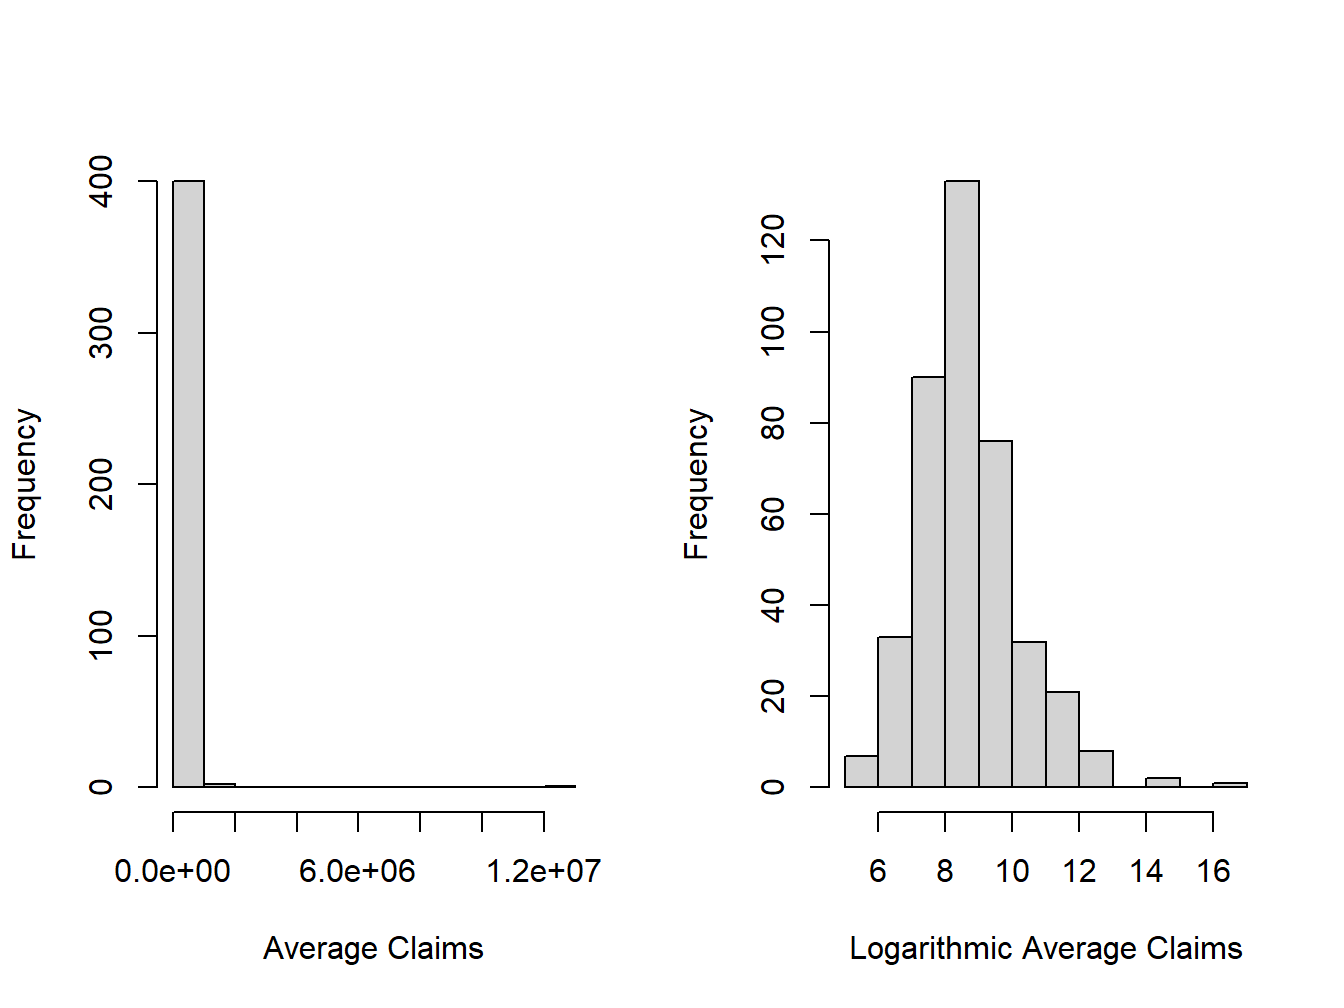
\includegraphics[width=0.8\linewidth]{LossDataAnalytics_files/figure-latex/SeverityFig-1} 

}

\caption{Distribution of Positive Average Severities}\label{fig:SeverityFig}
\end{figure}

R Code for Severity Distribution Table and Figures

\hypertarget{display.SeverityFig.2}{}
\begin{verbatim}
Insample <- read.csv("Data/PropertyFundInsample.csv", header=T, na.strings=c("."), stringsAsFactors=FALSE)
Insample2010 <- subset(Insample, Year==2010)
InsamplePos2010 <- subset(Insample2010, yAvg>0)
# Table
summary(InsamplePos2010$yAvg)
length(InsamplePos2010$yAvg)
# Figures
par(mfrow=c(1, 2))
hist(InsamplePos2010$yAvg, main="", xlab="Average Claims")
hist(log(InsamplePos2010$yAvg), main="", xlab="Logarithmic Average Claims")
\end{verbatim}

\subsection{Fund Rating Variables}\label{S:FundVariables}

Developing models to represent and manage the two outcome variables,
frequency and severity, is the focus of the early chapters of this text.
However, when actuaries and other financial analysts use those models,
they do so in the context of externally available variables. In general
statistical terminology, one might call these explanatory or predictor
variables; there are many other names in statistics, economics,
psychology, and other disciplines. Because of our insurance focus, we
call them \emph{rating variables} as they will be useful in setting
insurance rates and premiums.

We earlier considered a sample of 1,110 observations which may seem like
a lot. However, as we will seen in our forthcoming applications, because
of the preponderance of zeros and the skewed nature of claims, actuaries
typically yearn for more data. One common approach that we adopt here is
to examine outcomes from multiple years, thus increasing the sample
size. We will discuss the strengths and limitations of this strategy
later but, at this juncture, just want to show the reader how it works.

Specifically, Table \ref{tab:CoverageBCIM} shows that we now consider
policies over five years of data, years 2006, \ldots{}, 2010, inclusive.
The data begins in 2006 because there was a shift in claim coding in
2005 so that comparisons with earlier years are not helpful. To mitigate
the effect of open claims, we consider policy years prior to 2011. An
open claim means that all of the obligations are not known at the time
of the analysis; for some claims, such an injury to a person in an auto
accident or in the workplace, it can take years before costs are fully
known.

Table \ref{tab:CoverageBCIM} shows that the average claim varies over
time, especially with the high 2010 value due to a single large claim.
The total number of policyholders is steadily declining and, conversely,
the coverage is steadily increasing. The coverage variable is the amount
of coverage of the property and contents. Roughly, you can think of it
as the maximum possible payout of the insurer. For our immediate
purposes, it is our first rating variable. Other things being equal, we
would expect that policyholders with larger coverage will have larger
claims. We will make this vague idea much more precise as we proceed.

\begin{longtable}[]{@{}lrrrr@{}}
\caption{\label{tab:CoverageBCIM} Building and Contents Claims
Summary}\tabularnewline
\toprule
\begin{minipage}[b]{0.25\columnwidth}\raggedright\strut
Year\strut
\end{minipage} & \begin{minipage}[b]{0.14\columnwidth}\raggedleft\strut
Average Frequency\strut
\end{minipage} & \begin{minipage}[b]{0.13\columnwidth}\raggedleft\strut
Average Severity\strut
\end{minipage} & \begin{minipage}[b]{0.15\columnwidth}\raggedleft\strut
Average Coverage\strut
\end{minipage} & \begin{minipage}[b]{0.17\columnwidth}\raggedleft\strut
Number of Policyholders\strut
\end{minipage}\tabularnewline
\midrule
\endfirsthead
\toprule
\begin{minipage}[b]{0.25\columnwidth}\raggedright\strut
Year\strut
\end{minipage} & \begin{minipage}[b]{0.14\columnwidth}\raggedleft\strut
Average Frequency\strut
\end{minipage} & \begin{minipage}[b]{0.13\columnwidth}\raggedleft\strut
Average Severity\strut
\end{minipage} & \begin{minipage}[b]{0.15\columnwidth}\raggedleft\strut
Average Coverage\strut
\end{minipage} & \begin{minipage}[b]{0.17\columnwidth}\raggedleft\strut
Number of Policyholders\strut
\end{minipage}\tabularnewline
\midrule
\endhead
\begin{minipage}[t]{0.25\columnwidth}\raggedright\strut
2006\strut
\end{minipage} & \begin{minipage}[t]{0.14\columnwidth}\raggedleft\strut
0.951\strut
\end{minipage} & \begin{minipage}[t]{0.13\columnwidth}\raggedleft\strut
9,695\strut
\end{minipage} & \begin{minipage}[t]{0.15\columnwidth}\raggedleft\strut
32,498,186\strut
\end{minipage} & \begin{minipage}[t]{0.17\columnwidth}\raggedleft\strut
1,154\strut
\end{minipage}\tabularnewline
\begin{minipage}[t]{0.25\columnwidth}\raggedright\strut
2007\strut
\end{minipage} & \begin{minipage}[t]{0.14\columnwidth}\raggedleft\strut
1.167\strut
\end{minipage} & \begin{minipage}[t]{0.13\columnwidth}\raggedleft\strut
6,544\strut
\end{minipage} & \begin{minipage}[t]{0.15\columnwidth}\raggedleft\strut
35,275,949\strut
\end{minipage} & \begin{minipage}[t]{0.17\columnwidth}\raggedleft\strut
1,138\strut
\end{minipage}\tabularnewline
\begin{minipage}[t]{0.25\columnwidth}\raggedright\strut
2008\strut
\end{minipage} & \begin{minipage}[t]{0.14\columnwidth}\raggedleft\strut
0.974\strut
\end{minipage} & \begin{minipage}[t]{0.13\columnwidth}\raggedleft\strut
5,311\strut
\end{minipage} & \begin{minipage}[t]{0.15\columnwidth}\raggedleft\strut
37,267,485\strut
\end{minipage} & \begin{minipage}[t]{0.17\columnwidth}\raggedleft\strut
1,125\strut
\end{minipage}\tabularnewline
\begin{minipage}[t]{0.25\columnwidth}\raggedright\strut
2009\strut
\end{minipage} & \begin{minipage}[t]{0.14\columnwidth}\raggedleft\strut
1.219\strut
\end{minipage} & \begin{minipage}[t]{0.13\columnwidth}\raggedleft\strut
4,572\strut
\end{minipage} & \begin{minipage}[t]{0.15\columnwidth}\raggedleft\strut
40,355,382\strut
\end{minipage} & \begin{minipage}[t]{0.17\columnwidth}\raggedleft\strut
1,112\strut
\end{minipage}\tabularnewline
\begin{minipage}[t]{0.25\columnwidth}\raggedright\strut
2010\strut
\end{minipage} & \begin{minipage}[t]{0.14\columnwidth}\raggedleft\strut
1.241\strut
\end{minipage} & \begin{minipage}[t]{0.13\columnwidth}\raggedleft\strut
20,452\strut
\end{minipage} & \begin{minipage}[t]{0.15\columnwidth}\raggedleft\strut
41,242,070\strut
\end{minipage} & \begin{minipage}[t]{0.17\columnwidth}\raggedleft\strut
1,110\strut
\end{minipage}\tabularnewline
\bottomrule
\end{longtable}

R Code for Building and Contents Claims Summary

\hypertarget{display.CoverageBC.2}{}
\begin{verbatim}
Insample <- read.csv("Data/PropertyFundInsample.csv", header=T, na.strings=c("."), stringsAsFactors=FALSE)
library(doBy)
T1A <- summaryBy(Freq ~ Year, data = Insample, 
   FUN = function(x) { c(m = mean(x), num=length(x)) } )
T1B <- summaryBy(yAvg    ~ Year, data = Insample,   
   FUN = function(x) { c(m = mean(x), num=length(x)) } )
T1C <- summaryBy(BCcov    ~ Year, data = Insample,   
   FUN = function(x) { c(m = mean(x), num=length(x)) } )
Table1In <- cbind(T1A[1],T1A[2],T1B[2],T1C[2],T1A[3])
names(Table1In) <- c("Year", "Average Frequency","Average Severity", "Average","Number of Policyholders")
Table1In
\end{verbatim}

For a different look at this five-year sample, Table \ref{tab:DeductCov}
summarizes the distribution of our two outcomes, frequency and claims
amount. In each case, the average exceeds the median, suggesting that
the two distributions are right-skewed. In addition, the table
summarizes our continuous rating variables, coverage and deductible
amount. The table also suggests that these variables also have
right-skewed distributions.

\begin{longtable}[]{@{}lrrrr@{}}
\caption{\label{tab:DeductCov} Summary of Claim Frequency and Severity,
Deductibles, and Coverages}\tabularnewline
\toprule
\begin{minipage}[b]{0.19\columnwidth}\raggedright\strut
\strut
\end{minipage} & \begin{minipage}[b]{0.19\columnwidth}\raggedleft\strut
Minimum\strut
\end{minipage} & \begin{minipage}[b]{0.19\columnwidth}\raggedleft\strut
Median\strut
\end{minipage} & \begin{minipage}[b]{0.19\columnwidth}\raggedleft\strut
Average\strut
\end{minipage} & \begin{minipage}[b]{0.19\columnwidth}\raggedleft\strut
Maximum\strut
\end{minipage}\tabularnewline
\midrule
\endfirsthead
\toprule
\begin{minipage}[b]{0.19\columnwidth}\raggedright\strut
\strut
\end{minipage} & \begin{minipage}[b]{0.19\columnwidth}\raggedleft\strut
Minimum\strut
\end{minipage} & \begin{minipage}[b]{0.19\columnwidth}\raggedleft\strut
Median\strut
\end{minipage} & \begin{minipage}[b]{0.19\columnwidth}\raggedleft\strut
Average\strut
\end{minipage} & \begin{minipage}[b]{0.19\columnwidth}\raggedleft\strut
Maximum\strut
\end{minipage}\tabularnewline
\midrule
\endhead
\begin{minipage}[t]{0.23\columnwidth}\raggedright\strut
Claim Frequency\strut
\end{minipage} & \begin{minipage}[t]{0.12\columnwidth}\raggedleft\strut
0\strut
\end{minipage} & \begin{minipage}[t]{0.11\columnwidth}\raggedleft\strut
0\strut
\end{minipage} & \begin{minipage}[t]{0.12\columnwidth}\raggedleft\strut
1.109\strut
\end{minipage} & \begin{minipage}[t]{0.14\columnwidth}\raggedleft\strut
263\strut
\end{minipage}\tabularnewline
\begin{minipage}[t]{0.23\columnwidth}\raggedright\strut
Claim Severity\strut
\end{minipage} & \begin{minipage}[t]{0.12\columnwidth}\raggedleft\strut
0\strut
\end{minipage} & \begin{minipage}[t]{0.11\columnwidth}\raggedleft\strut
0\strut
\end{minipage} & \begin{minipage}[t]{0.12\columnwidth}\raggedleft\strut
9,292\strut
\end{minipage} & \begin{minipage}[t]{0.14\columnwidth}\raggedleft\strut
12,922,218\strut
\end{minipage}\tabularnewline
\begin{minipage}[t]{0.23\columnwidth}\raggedright\strut
Deductible\strut
\end{minipage} & \begin{minipage}[t]{0.12\columnwidth}\raggedleft\strut
500\strut
\end{minipage} & \begin{minipage}[t]{0.11\columnwidth}\raggedleft\strut
1,000\strut
\end{minipage} & \begin{minipage}[t]{0.12\columnwidth}\raggedleft\strut
3,365\strut
\end{minipage} & \begin{minipage}[t]{0.14\columnwidth}\raggedleft\strut
100,000\strut
\end{minipage}\tabularnewline
\begin{minipage}[t]{0.23\columnwidth}\raggedright\strut
Coverage (000's)\strut
\end{minipage} & \begin{minipage}[t]{0.12\columnwidth}\raggedleft\strut
8.937\strut
\end{minipage} & \begin{minipage}[t]{0.11\columnwidth}\raggedleft\strut
11,354\strut
\end{minipage} & \begin{minipage}[t]{0.12\columnwidth}\raggedleft\strut
37,281\strut
\end{minipage} & \begin{minipage}[t]{0.14\columnwidth}\raggedleft\strut
2,444,797\strut
\end{minipage}\tabularnewline
\bottomrule
\end{longtable}

R Code for Summary of Claim Frequency and Severity, Deductibles, and
Coverages

\hypertarget{display.DeductCov.2}{}
\begin{verbatim}
Insample <- read.csv("Data/PropertyFundInsample.csv", header=T, na.strings=c("."), stringsAsFactors=FALSE)
t1<- summaryBy(Insample$Freq ~ 1, data = Insample, 
   FUN = function(x) { c(ma=min(x), m1=median(x),m=mean(x),mb=max(x)) } )
names(t1) <- c("Minimum", "Median","Average", "Maximum")
t2 <- summaryBy(Insample$yAvg ~ 1, data = Insample, 
   FUN = function(x) { c(ma=min(x), m1=median(x), m=mean(x),mb=max(x)) } )
names(t2) <- c("Minimum", "Median","Average", "Maximum")
t3 <- summaryBy(Deduct ~ 1, data = Insample, 
   FUN = function(x) { c(ma=min(x), m1=median(x), m=mean(x),mb=max(x)) } )
names(t3) <- c("Minimum", "Median","Average", "Maximum")
t4 <- summaryBy(BCcov/1000 ~ 1, data = Insample, 
   FUN = function(x) { c(ma=min(x), m1=median(x), m=mean(x),mb=max(x)) } )
names(t4) <- c("Minimum", "Median","Average", "Maximum")
Table2 <- rbind(t1,t2,t3,t4)
Table2a <- round(Table2,3)
Rowlable <- rbind("Claim Frequency","Claim Severity","Deductible","Coverage (000's)")
Table2aa <- cbind(Rowlable,as.matrix(Table2a))
Table2aa
\end{verbatim}

Table \ref{tab:VarDescr} describes the rating variables considered in
this chapter. To handle the skewness, we henceforth focus on logarithmic
transformations of coverage and deductibles. To get a sense of the
relationship between the non-continuous rating variables and claims,
Table \ref{tab:ClaimRateVar} relates the claims outcomes to these
categorical variables. Table \ref{tab:ClaimRateVar} suggests substantial
variation in the claim frequency and average severity of the claims by
entity type. It also demonstrates higher frequency and severity for the
\({\tt Fire5}\) variable and the reverse for the \({\tt NoClaimCredit}\)
variable. The relationship for the \({\tt Fire5}\) variable is
counter-intuitive in that one would expect lower claim amounts for those
policyholders in areas with better public protection (when the
protection code is five or less). Naturally, there are other variables
that influence this relationship. We will see that these background
variables are accounted for in the subsequent multivariate regression
analysis, which yields an intuitive, appealing (negative) sign for the
\({\tt Fire5}\) variable.

Table: \label{tab:VarDescr} Description of Rating Variables

\[{\small \begin{matrix}
\begin{array}{ l | l}
\hline
Variable    & Description \\
\hline
\text{EntityType}   & \text{Categorical variable that is one of six types:  (Village, City,} \\
& ~~~~ \text{County, Misc, School, or Town)} \\
\text{LnCoverage}   & \text{Total building and content coverage, in logarithmic millions of dollars}\\
\text{LnDeduct}     & \text{Deductible, in logarithmic dollars} \\
\text{AlarmCredit}  & \text{Categorical variable that is one of four types:  (0, 5, 10, or 15)} \\
 &  ~~~~   \text{for automatic smoke alarms in main rooms} \\
\text{NoClaimCredit}    & \text{Binary variable to indicate no claims in the past two years} \\
\text{Fire5 }           & \text{Binary variable to indicate the fire class is below 5} \\
& ~~~~ \text{(The range of fire class is 0 to 10} \\
\hline
\end{array}
\end{matrix}}\]

\begin{longtable}[]{@{}lrrr@{}}
\caption{\label{tab:ClaimRateVar} Claims Summary by Entity Type, Fire Class,
and No Claim Credit}\tabularnewline
\toprule
\begin{minipage}[b]{0.27\columnwidth}\raggedright\strut
Variable\strut
\end{minipage} & \begin{minipage}[b]{0.15\columnwidth}\raggedleft\strut
Number of Policies\strut
\end{minipage} & \begin{minipage}[b]{0.15\columnwidth}\raggedleft\strut
Claim Frequency\strut
\end{minipage} & \begin{minipage}[b]{0.15\columnwidth}\raggedleft\strut
Average Severity\strut
\end{minipage}\tabularnewline
\midrule
\endfirsthead
\toprule
\begin{minipage}[b]{0.27\columnwidth}\raggedright\strut
Variable\strut
\end{minipage} & \begin{minipage}[b]{0.15\columnwidth}\raggedleft\strut
Number of Policies\strut
\end{minipage} & \begin{minipage}[b]{0.15\columnwidth}\raggedleft\strut
Claim Frequency\strut
\end{minipage} & \begin{minipage}[b]{0.15\columnwidth}\raggedleft\strut
Average Severity\strut
\end{minipage}\tabularnewline
\midrule
\endhead
\begin{minipage}[t]{0.24\columnwidth}\raggedright\strut
\emph{EntityType}\strut
\end{minipage} & \begin{minipage}[t]{0.24\columnwidth}\raggedleft\strut
\strut
\end{minipage} & \begin{minipage}[t]{0.24\columnwidth}\raggedleft\strut
\strut
\end{minipage} & \begin{minipage}[t]{0.24\columnwidth}\raggedleft\strut
\strut
\end{minipage}\tabularnewline
\begin{minipage}[t]{0.27\columnwidth}\raggedright\strut
Village\strut
\end{minipage} & \begin{minipage}[t]{0.15\columnwidth}\raggedleft\strut
1,341\strut
\end{minipage} & \begin{minipage}[t]{0.15\columnwidth}\raggedleft\strut
0.452\strut
\end{minipage} & \begin{minipage}[t]{0.15\columnwidth}\raggedleft\strut
10,645\strut
\end{minipage}\tabularnewline
\begin{minipage}[t]{0.27\columnwidth}\raggedright\strut
City\strut
\end{minipage} & \begin{minipage}[t]{0.15\columnwidth}\raggedleft\strut
793\strut
\end{minipage} & \begin{minipage}[t]{0.15\columnwidth}\raggedleft\strut
1.941\strut
\end{minipage} & \begin{minipage}[t]{0.15\columnwidth}\raggedleft\strut
16,924\strut
\end{minipage}\tabularnewline
\begin{minipage}[t]{0.27\columnwidth}\raggedright\strut
County\strut
\end{minipage} & \begin{minipage}[t]{0.15\columnwidth}\raggedleft\strut
328\strut
\end{minipage} & \begin{minipage}[t]{0.15\columnwidth}\raggedleft\strut
4.899\strut
\end{minipage} & \begin{minipage}[t]{0.15\columnwidth}\raggedleft\strut
15,453\strut
\end{minipage}\tabularnewline
\begin{minipage}[t]{0.27\columnwidth}\raggedright\strut
Misc\strut
\end{minipage} & \begin{minipage}[t]{0.15\columnwidth}\raggedleft\strut
609\strut
\end{minipage} & \begin{minipage}[t]{0.15\columnwidth}\raggedleft\strut
0.186\strut
\end{minipage} & \begin{minipage}[t]{0.15\columnwidth}\raggedleft\strut
43,036\strut
\end{minipage}\tabularnewline
\begin{minipage}[t]{0.27\columnwidth}\raggedright\strut
School\strut
\end{minipage} & \begin{minipage}[t]{0.15\columnwidth}\raggedleft\strut
1,597\strut
\end{minipage} & \begin{minipage}[t]{0.15\columnwidth}\raggedleft\strut
1.434\strut
\end{minipage} & \begin{minipage}[t]{0.15\columnwidth}\raggedleft\strut
64,346\strut
\end{minipage}\tabularnewline
\begin{minipage}[t]{0.27\columnwidth}\raggedright\strut
Town\strut
\end{minipage} & \begin{minipage}[t]{0.15\columnwidth}\raggedleft\strut
971\strut
\end{minipage} & \begin{minipage}[t]{0.15\columnwidth}\raggedleft\strut
0.103\strut
\end{minipage} & \begin{minipage}[t]{0.15\columnwidth}\raggedleft\strut
19,831\strut
\end{minipage}\tabularnewline
\begin{minipage}[t]{0.27\columnwidth}\raggedright\strut
Fire5=0\strut
\end{minipage} & \begin{minipage}[t]{0.15\columnwidth}\raggedleft\strut
2,508\strut
\end{minipage} & \begin{minipage}[t]{0.15\columnwidth}\raggedleft\strut
0.502\strut
\end{minipage} & \begin{minipage}[t]{0.15\columnwidth}\raggedleft\strut
13,935\strut
\end{minipage}\tabularnewline
\begin{minipage}[t]{0.27\columnwidth}\raggedright\strut
Fire5=1\strut
\end{minipage} & \begin{minipage}[t]{0.15\columnwidth}\raggedleft\strut
3,131\strut
\end{minipage} & \begin{minipage}[t]{0.15\columnwidth}\raggedleft\strut
1.596\strut
\end{minipage} & \begin{minipage}[t]{0.15\columnwidth}\raggedleft\strut
41,421\strut
\end{minipage}\tabularnewline
\begin{minipage}[t]{0.27\columnwidth}\raggedright\strut
NoClaimCredit=0\strut
\end{minipage} & \begin{minipage}[t]{0.15\columnwidth}\raggedleft\strut
3,786\strut
\end{minipage} & \begin{minipage}[t]{0.15\columnwidth}\raggedleft\strut
1.501\strut
\end{minipage} & \begin{minipage}[t]{0.15\columnwidth}\raggedleft\strut
31,365\strut
\end{minipage}\tabularnewline
\begin{minipage}[t]{0.27\columnwidth}\raggedright\strut
NoClaimCredit=1\strut
\end{minipage} & \begin{minipage}[t]{0.15\columnwidth}\raggedleft\strut
1,853\strut
\end{minipage} & \begin{minipage}[t]{0.15\columnwidth}\raggedleft\strut
0.310\strut
\end{minipage} & \begin{minipage}[t]{0.15\columnwidth}\raggedleft\strut
30,499\strut
\end{minipage}\tabularnewline
\begin{minipage}[t]{0.27\columnwidth}\raggedright\strut
Total\strut
\end{minipage} & \begin{minipage}[t]{0.15\columnwidth}\raggedleft\strut
5,639\strut
\end{minipage} & \begin{minipage}[t]{0.15\columnwidth}\raggedleft\strut
1.109\strut
\end{minipage} & \begin{minipage}[t]{0.15\columnwidth}\raggedleft\strut
31,206\strut
\end{minipage}\tabularnewline
\bottomrule
\end{longtable}

R Code for Claims Summary by Entity Type, Fire Class, and No Claim
Credit

\hypertarget{display.ClaimRateVar.2}{}
\begin{verbatim}
ByVarSumm<-function(datasub){
  tempA <- summaryBy(Freq    ~ 1 , data = datasub,   
     FUN = function(x) { c(m = mean(x), num=length(x)) } )
  datasub1 <-  subset(datasub, yAvg>0)
  tempB <- summaryBy(yAvg   ~ 1, data = datasub1,FUN = function(x) { c(m = mean(x)) } )
  tempC <- merge(tempA,tempB,all.x=T)[c(2,1,3)]
  tempC1 <- as.matrix(tempC)
  return(tempC1)
  }
datasub <-  subset(Insample, TypeVillage == 1);   
t1 <- ByVarSumm(datasub)
datasub <-  subset(Insample, TypeCity == 1);      
t2 <- ByVarSumm(datasub)
datasub <-  subset(Insample, TypeCounty == 1);   
t3 <- ByVarSumm(datasub)
datasub <-  subset(Insample, TypeMisc == 1);      
t4 <- ByVarSumm(datasub)
datasub <-  subset(Insample, TypeSchool == 1);    
t5 <- ByVarSumm(datasub)
datasub <-  subset(Insample, TypeTown == 1);      
t6 <- ByVarSumm(datasub)
datasub <-  subset(Insample, Fire5 == 0);                      
t7 <- ByVarSumm(datasub)
datasub <-  subset(Insample, Fire5 == 1);                      
t8 <- ByVarSumm(datasub)
datasub <-  subset(Insample, Insample$NoClaimCredit == 0);
t9 <- ByVarSumm(datasub)
datasub <-  subset(Insample, Insample$NoClaimCredit == 1);
t10 <- ByVarSumm(datasub)
t11 <- ByVarSumm(Insample)

Tablea <- rbind(t1,t2,t3,t4,t5,t6,t7,t8,t9,t10,t11)
Tableaa <- round(Tablea,3)
Rowlable <- rbind("Village","City","County","Misc","School",
          "Town","Fire5--No","Fire5--Yes","NoClaimCredit--No",
        "NoClaimCredit--Yes","Total")
Table4 <- cbind(Rowlable,as.matrix(Tableaa))
Table4
\end{verbatim}

Table \ref{tab:RateAlarmCredit} shows the claims experience by alarm
credit. It underscores the difficulty of examining variables
individually. For example, when looking at the experience for all
entities, we see that policyholders with no alarm credit have on average
lower frequency and severity than policyholders with the highest (15\%,
with 24/7 monitoring by a fire station or security company) alarm
credit. In particular, when we look at the entity type School, the
frequency is 0.422 and the severity 25,257 for no alarm credit, whereas
for the highest alarm level it is 2.008 and 85,140. This may simply
imply that entities with more claims are the ones that are likely to
have an alarm system. Summary tables do not examine multivariate
effects; for example, Table \ref{tab:ClaimRateVar} ignores the effect of
size (as we measure through coverage amounts) that affect claims.

\begin{longtable}[]{@{}lrrrrrr@{}}
\caption{\label{tab:RateAlarmCredit} Claims Summary by Entity Type and Alarm
Credit Category}\tabularnewline
\toprule
\begin{minipage}[b]{0.10\columnwidth}\raggedright\strut
Entity Type\strut
\end{minipage} & \begin{minipage}[b]{0.12\columnwidth}\raggedleft\strut
Claim Frequency\strut
\end{minipage} & \begin{minipage}[b]{0.11\columnwidth}\raggedleft\strut
Avg. Severity\strut
\end{minipage} & \begin{minipage}[b]{0.11\columnwidth}\raggedleft\strut
Num. Policies\strut
\end{minipage} & \begin{minipage}[b]{0.12\columnwidth}\raggedleft\strut
Claim Frequency\strut
\end{minipage} & \begin{minipage}[b]{0.11\columnwidth}\raggedleft\strut
Avg. Severity\strut
\end{minipage} & \begin{minipage}[b]{0.11\columnwidth}\raggedleft\strut
Num. Policies\strut
\end{minipage}\tabularnewline
\midrule
\endfirsthead
\toprule
\begin{minipage}[b]{0.10\columnwidth}\raggedright\strut
Entity Type\strut
\end{minipage} & \begin{minipage}[b]{0.12\columnwidth}\raggedleft\strut
Claim Frequency\strut
\end{minipage} & \begin{minipage}[b]{0.11\columnwidth}\raggedleft\strut
Avg. Severity\strut
\end{minipage} & \begin{minipage}[b]{0.11\columnwidth}\raggedleft\strut
Num. Policies\strut
\end{minipage} & \begin{minipage}[b]{0.12\columnwidth}\raggedleft\strut
Claim Frequency\strut
\end{minipage} & \begin{minipage}[b]{0.11\columnwidth}\raggedleft\strut
Avg. Severity\strut
\end{minipage} & \begin{minipage}[b]{0.11\columnwidth}\raggedleft\strut
Num. Policies\strut
\end{minipage}\tabularnewline
\midrule
\endhead
\begin{minipage}[t]{0.10\columnwidth}\raggedright\strut
Village\strut
\end{minipage} & \begin{minipage}[t]{0.12\columnwidth}\raggedleft\strut
0.326\strut
\end{minipage} & \begin{minipage}[t]{0.11\columnwidth}\raggedleft\strut
11,078\strut
\end{minipage} & \begin{minipage}[t]{0.11\columnwidth}\raggedleft\strut
829\strut
\end{minipage} & \begin{minipage}[t]{0.12\columnwidth}\raggedleft\strut
0.278\strut
\end{minipage} & \begin{minipage}[t]{0.11\columnwidth}\raggedleft\strut
8,086\strut
\end{minipage} & \begin{minipage}[t]{0.11\columnwidth}\raggedleft\strut
54\strut
\end{minipage}\tabularnewline
\begin{minipage}[t]{0.10\columnwidth}\raggedright\strut
City\strut
\end{minipage} & \begin{minipage}[t]{0.12\columnwidth}\raggedleft\strut
0.893\strut
\end{minipage} & \begin{minipage}[t]{0.11\columnwidth}\raggedleft\strut
7,576\strut
\end{minipage} & \begin{minipage}[t]{0.11\columnwidth}\raggedleft\strut
244\strut
\end{minipage} & \begin{minipage}[t]{0.12\columnwidth}\raggedleft\strut
2.077\strut
\end{minipage} & \begin{minipage}[t]{0.11\columnwidth}\raggedleft\strut
4,150\strut
\end{minipage} & \begin{minipage}[t]{0.11\columnwidth}\raggedleft\strut
13\strut
\end{minipage}\tabularnewline
\begin{minipage}[t]{0.10\columnwidth}\raggedright\strut
County\strut
\end{minipage} & \begin{minipage}[t]{0.12\columnwidth}\raggedleft\strut
2.140\strut
\end{minipage} & \begin{minipage}[t]{0.11\columnwidth}\raggedleft\strut
16,013\strut
\end{minipage} & \begin{minipage}[t]{0.11\columnwidth}\raggedleft\strut
50\strut
\end{minipage} & \begin{minipage}[t]{0.12\columnwidth}\raggedleft\strut
-\strut
\end{minipage} & \begin{minipage}[t]{0.11\columnwidth}\raggedleft\strut
-\strut
\end{minipage} & \begin{minipage}[t]{0.11\columnwidth}\raggedleft\strut
1\strut
\end{minipage}\tabularnewline
\begin{minipage}[t]{0.10\columnwidth}\raggedright\strut
Misc\strut
\end{minipage} & \begin{minipage}[t]{0.12\columnwidth}\raggedleft\strut
0.117\strut
\end{minipage} & \begin{minipage}[t]{0.11\columnwidth}\raggedleft\strut
15,122\strut
\end{minipage} & \begin{minipage}[t]{0.11\columnwidth}\raggedleft\strut
386\strut
\end{minipage} & \begin{minipage}[t]{0.12\columnwidth}\raggedleft\strut
0.278\strut
\end{minipage} & \begin{minipage}[t]{0.11\columnwidth}\raggedleft\strut
13,064\strut
\end{minipage} & \begin{minipage}[t]{0.11\columnwidth}\raggedleft\strut
18\strut
\end{minipage}\tabularnewline
\begin{minipage}[t]{0.10\columnwidth}\raggedright\strut
School\strut
\end{minipage} & \begin{minipage}[t]{0.12\columnwidth}\raggedleft\strut
0.422\strut
\end{minipage} & \begin{minipage}[t]{0.11\columnwidth}\raggedleft\strut
25,523\strut
\end{minipage} & \begin{minipage}[t]{0.11\columnwidth}\raggedleft\strut
294\strut
\end{minipage} & \begin{minipage}[t]{0.12\columnwidth}\raggedleft\strut
0.410\strut
\end{minipage} & \begin{minipage}[t]{0.11\columnwidth}\raggedleft\strut
14,575\strut
\end{minipage} & \begin{minipage}[t]{0.11\columnwidth}\raggedleft\strut
122\strut
\end{minipage}\tabularnewline
\begin{minipage}[t]{0.10\columnwidth}\raggedright\strut
Town\strut
\end{minipage} & \begin{minipage}[t]{0.12\columnwidth}\raggedleft\strut
0.083\strut
\end{minipage} & \begin{minipage}[t]{0.11\columnwidth}\raggedleft\strut
25,257\strut
\end{minipage} & \begin{minipage}[t]{0.11\columnwidth}\raggedleft\strut
808\strut
\end{minipage} & \begin{minipage}[t]{0.12\columnwidth}\raggedleft\strut
0.194\strut
\end{minipage} & \begin{minipage}[t]{0.11\columnwidth}\raggedleft\strut
3,937\strut
\end{minipage} & \begin{minipage}[t]{0.11\columnwidth}\raggedleft\strut
31\strut
\end{minipage}\tabularnewline
\begin{minipage}[t]{0.10\columnwidth}\raggedright\strut
Total\strut
\end{minipage} & \begin{minipage}[t]{0.12\columnwidth}\raggedleft\strut
0.318\strut
\end{minipage} & \begin{minipage}[t]{0.11\columnwidth}\raggedleft\strut
15,118\strut
\end{minipage} & \begin{minipage}[t]{0.11\columnwidth}\raggedleft\strut
2,611\strut
\end{minipage} & \begin{minipage}[t]{0.12\columnwidth}\raggedleft\strut
0.431\strut
\end{minipage} & \begin{minipage}[t]{0.11\columnwidth}\raggedleft\strut
10,762\strut
\end{minipage} & \begin{minipage}[t]{0.11\columnwidth}\raggedleft\strut
239\strut
\end{minipage}\tabularnewline
\bottomrule
\end{longtable}

\begin{longtable}[]{@{}lrrrrrr@{}}
\caption{Claims Summary by Entity Type and Alarm Credit
Category}\tabularnewline
\toprule
\begin{minipage}[b]{0.10\columnwidth}\raggedright\strut
Entity Type\strut
\end{minipage} & \begin{minipage}[b]{0.12\columnwidth}\raggedleft\strut
Claim Frequency\strut
\end{minipage} & \begin{minipage}[b]{0.11\columnwidth}\raggedleft\strut
Avg. Severity\strut
\end{minipage} & \begin{minipage}[b]{0.11\columnwidth}\raggedleft\strut
Num. Policies\strut
\end{minipage} & \begin{minipage}[b]{0.12\columnwidth}\raggedleft\strut
Claim Frequency\strut
\end{minipage} & \begin{minipage}[b]{0.11\columnwidth}\raggedleft\strut
Avg. Severity\strut
\end{minipage} & \begin{minipage}[b]{0.11\columnwidth}\raggedleft\strut
Num. Policies\strut
\end{minipage}\tabularnewline
\midrule
\endfirsthead
\toprule
\begin{minipage}[b]{0.10\columnwidth}\raggedright\strut
Entity Type\strut
\end{minipage} & \begin{minipage}[b]{0.12\columnwidth}\raggedleft\strut
Claim Frequency\strut
\end{minipage} & \begin{minipage}[b]{0.11\columnwidth}\raggedleft\strut
Avg. Severity\strut
\end{minipage} & \begin{minipage}[b]{0.11\columnwidth}\raggedleft\strut
Num. Policies\strut
\end{minipage} & \begin{minipage}[b]{0.12\columnwidth}\raggedleft\strut
Claim Frequency\strut
\end{minipage} & \begin{minipage}[b]{0.11\columnwidth}\raggedleft\strut
Avg. Severity\strut
\end{minipage} & \begin{minipage}[b]{0.11\columnwidth}\raggedleft\strut
Num. Policies\strut
\end{minipage}\tabularnewline
\midrule
\endhead
\begin{minipage}[t]{0.10\columnwidth}\raggedright\strut
Village\strut
\end{minipage} & \begin{minipage}[t]{0.12\columnwidth}\raggedleft\strut
0.500\strut
\end{minipage} & \begin{minipage}[t]{0.11\columnwidth}\raggedleft\strut
8,792\strut
\end{minipage} & \begin{minipage}[t]{0.11\columnwidth}\raggedleft\strut
50\strut
\end{minipage} & \begin{minipage}[t]{0.12\columnwidth}\raggedleft\strut
0.725\strut
\end{minipage} & \begin{minipage}[t]{0.11\columnwidth}\raggedleft\strut
10,544\strut
\end{minipage} & \begin{minipage}[t]{0.11\columnwidth}\raggedleft\strut
408\strut
\end{minipage}\tabularnewline
\begin{minipage}[t]{0.10\columnwidth}\raggedright\strut
City\strut
\end{minipage} & \begin{minipage}[t]{0.12\columnwidth}\raggedleft\strut
1.258\strut
\end{minipage} & \begin{minipage}[t]{0.11\columnwidth}\raggedleft\strut
8,625\strut
\end{minipage} & \begin{minipage}[t]{0.11\columnwidth}\raggedleft\strut
31\strut
\end{minipage} & \begin{minipage}[t]{0.12\columnwidth}\raggedleft\strut
2.485\strut
\end{minipage} & \begin{minipage}[t]{0.11\columnwidth}\raggedleft\strut
20,470\strut
\end{minipage} & \begin{minipage}[t]{0.11\columnwidth}\raggedleft\strut
505\strut
\end{minipage}\tabularnewline
\begin{minipage}[t]{0.10\columnwidth}\raggedright\strut
County\strut
\end{minipage} & \begin{minipage}[t]{0.12\columnwidth}\raggedleft\strut
2.125\strut
\end{minipage} & \begin{minipage}[t]{0.11\columnwidth}\raggedleft\strut
11,688\strut
\end{minipage} & \begin{minipage}[t]{0.11\columnwidth}\raggedleft\strut
8\strut
\end{minipage} & \begin{minipage}[t]{0.12\columnwidth}\raggedleft\strut
5.513\strut
\end{minipage} & \begin{minipage}[t]{0.11\columnwidth}\raggedleft\strut
15,476\strut
\end{minipage} & \begin{minipage}[t]{0.11\columnwidth}\raggedleft\strut
269\strut
\end{minipage}\tabularnewline
\begin{minipage}[t]{0.10\columnwidth}\raggedright\strut
Misc\strut
\end{minipage} & \begin{minipage}[t]{0.12\columnwidth}\raggedleft\strut
0.077\strut
\end{minipage} & \begin{minipage}[t]{0.11\columnwidth}\raggedleft\strut
3,923\strut
\end{minipage} & \begin{minipage}[t]{0.11\columnwidth}\raggedleft\strut
26\strut
\end{minipage} & \begin{minipage}[t]{0.12\columnwidth}\raggedleft\strut
0.341\strut
\end{minipage} & \begin{minipage}[t]{0.11\columnwidth}\raggedleft\strut
87,021\strut
\end{minipage} & \begin{minipage}[t]{0.11\columnwidth}\raggedleft\strut
179\strut
\end{minipage}\tabularnewline
\begin{minipage}[t]{0.10\columnwidth}\raggedright\strut
School\strut
\end{minipage} & \begin{minipage}[t]{0.12\columnwidth}\raggedleft\strut
0.488\strut
\end{minipage} & \begin{minipage}[t]{0.11\columnwidth}\raggedleft\strut
11,597\strut
\end{minipage} & \begin{minipage}[t]{0.11\columnwidth}\raggedleft\strut
168\strut
\end{minipage} & \begin{minipage}[t]{0.12\columnwidth}\raggedleft\strut
2.008\strut
\end{minipage} & \begin{minipage}[t]{0.11\columnwidth}\raggedleft\strut
85,140\strut
\end{minipage} & \begin{minipage}[t]{0.11\columnwidth}\raggedleft\strut
1,013\strut
\end{minipage}\tabularnewline
\begin{minipage}[t]{0.10\columnwidth}\raggedright\strut
Town\strut
\end{minipage} & \begin{minipage}[t]{0.12\columnwidth}\raggedleft\strut
0.091\strut
\end{minipage} & \begin{minipage}[t]{0.11\columnwidth}\raggedleft\strut
2,338\strut
\end{minipage} & \begin{minipage}[t]{0.11\columnwidth}\raggedleft\strut
44\strut
\end{minipage} & \begin{minipage}[t]{0.12\columnwidth}\raggedleft\strut
0.261\strut
\end{minipage} & \begin{minipage}[t]{0.11\columnwidth}\raggedleft\strut
9,490\strut
\end{minipage} & \begin{minipage}[t]{0.11\columnwidth}\raggedleft\strut
88\strut
\end{minipage}\tabularnewline
\begin{minipage}[t]{0.10\columnwidth}\raggedright\strut
Total\strut
\end{minipage} & \begin{minipage}[t]{0.12\columnwidth}\raggedleft\strut
0.517\strut
\end{minipage} & \begin{minipage}[t]{0.11\columnwidth}\raggedleft\strut
10,194\strut
\end{minipage} & \begin{minipage}[t]{0.11\columnwidth}\raggedleft\strut
327\strut
\end{minipage} & \begin{minipage}[t]{0.12\columnwidth}\raggedleft\strut
2.093\strut
\end{minipage} & \begin{minipage}[t]{0.11\columnwidth}\raggedleft\strut
41,458\strut
\end{minipage} & \begin{minipage}[t]{0.11\columnwidth}\raggedleft\strut
2,462\strut
\end{minipage}\tabularnewline
\bottomrule
\end{longtable}

R Code for Claims Summary by Entity Type and Alarm Credit Category

\hypertarget{display.RateAlarmCredit.2}{}
\begin{verbatim}
#Claims Summary by Entity Type and Alarm Credit
ByVarSumm<-function(datasub){
  tempA <- summaryBy(Freq    ~ AC00 , data = datasub,   
                     FUN = function(x) { c(m = mean(x), num=length(x)) } )
  datasub1 <-  subset(datasub, yAvg>0)
  if(nrow(datasub1)==0) { n<-nrow(datasub)
    return(c(0,0,n))
  } else 
  {
    tempB <- summaryBy(yAvg   ~ AC00, data = datasub1,
                       FUN = function(x) { c(m = mean(x)) } )
    tempC <- merge(tempA,tempB,all.x=T)[c(2,4,3)]
    tempC1 <- as.matrix(tempC)
    return(tempC1)
  }
}
AlarmC <- 1*(Insample$AC00==1) + 2*(Insample$AC05==1)+ 3*(Insample$AC10==1)+ 4*(Insample$AC15==1)
ByVarCredit<-function(ACnum){
datasub <-  subset(Insample, TypeVillage == 1 & AlarmC == ACnum); 
  t1 <- ByVarSumm(datasub)
datasub <-  subset(Insample, TypeCity == 1 & AlarmC == ACnum);      
  t2 <- ByVarSumm(datasub)
datasub <-  subset(Insample, TypeCounty == 1 & AlarmC == ACnum);   
  t3 <- ByVarSumm(datasub)
datasub <-  subset(Insample, TypeMisc == 1 & AlarmC == ACnum);
  t4 <- ByVarSumm(datasub)
datasub <-  subset(Insample, TypeSchool == 1 & AlarmC == ACnum);    
  t5 <- ByVarSumm(datasub)
datasub <-  subset(Insample, TypeTown == 1 & AlarmC ==ACnum);      
  t6 <- ByVarSumm(datasub)
datasub <-  subset(Insample, AlarmC == ACnum);  
  t7 <- ByVarSumm(datasub)
Tablea <- rbind(t1,t2,t3,t4,t5,t6,t7)
Tableaa <- round(Tablea,3)
Rowlable <- rbind("Village","City","County","Misc","School",
                  "Town","Total")
Table4 <- cbind(Rowlable,as.matrix(Tableaa))
}
Table4a <- ByVarCredit(1)    #Claims Summary by Entity Type and Alarm Credit==00
Table4b <- ByVarCredit(2)    #Claims Summary by Entity Type and Alarm Credit==05 
Table4c <- ByVarCredit(3)    #Claims Summary by Entity Type and Alarm Credit==10
Table4d <- ByVarCredit(4)    #Claims Summary by Entity Type and Alarm Credit==15
\end{verbatim}

\subsection{Fund Operations}\label{fund-operations}

We have now seen the Fund's two outcome variables, a count variable for
the number of claims and a continuous variable for the claims amount. We
have also introduced a continuous rating variable, coverage, discrete
quantitative variable, (logarithmic) deductibles, two binary rating
variable, no claims credit and fire class, as well as two categorical
rating variables, entity type and alarm credit. Subsequent chapters will
explain how to analyze and model the distribution of these variables and
their relationships. Before getting into these technical details, let us
first think about where we want to go. General insurance company
functional areas are described in Section \ref{S:PredModApps}; let us
now think about how these areas might apply in the context of the
property fund.

\subsubsection*{Initiating Insurance}\label{initiating-insurance-1}
\addcontentsline{toc}{subsubsection}{Initiating Insurance}

Because this is a government sponsored fund, we do not have to worry
about selecting good or avoiding poor risks; the fund is not allowed to
deny a coverage application from a qualified local government entity. If
we do not have to underwrite, what about how much to charge?

We might look at the most recent experience in 2010, where the total
fund claims were approximately 28.16 million USD
(\(=1377 \text{ claims} \times 20452 \text{ average severity}\)).
Dividing that among 1,110 policyholders, that suggests a rate of 24,370
( \(\approx\) 28,160,000/1110). However, 2010 was a bad year; using the
same method, our premium would be much lower based on 2009 data. This
swing in premiums would defeat the primary purpose of the fund, to allow
for a steady charge that local property managers could utilize in their
budgets.

Having a single price for all policyholders is nice but hardly seems
fair. For example, Table \ref{tab:ClaimRateVar} suggests that Schools
have much higher claims than other entities and so should pay more.
However, simply doing the calculation on an entity by entity basis is
not right either. For example, we saw in Table \ref{tab:RateAlarmCredit}
that had we used this strategy, entities with a 15\% alarm credit (for
good behavior, having top alarm systems) would actually wind up paying
more.

So, we have the data for thinking about the appropriate rates to charge
but will need to dig deeper into the analysis. We will explore this
topic further in Chapter 6 on \emph{premium calculation fundamentals}.
Selecting appropriate risks is introduced in Chapter 7 on \emph{risk
classification}.

\subsubsection*{Renewing Insurance}\label{renewing-insurance-1}
\addcontentsline{toc}{subsubsection}{Renewing Insurance}

Although property insurance is typically a one-year contract, Table
\ref{tab:CoverageBCIM} suggests that policyholders tend to renew; this
is typical of general insurance. For renewing policyholders, in addition
to their rating variables we have their claims history and this claims
history can be a good predictor of future claims. For example, Table
\ref{tab:CoverageBCIM} shows that policyholders without a claim in the
last two years had much lower claim frequencies than those with at least
one accident (0.310 compared to 1.501); a lower predicted frequency
typically results in a lower premium. This is why it is common for
insurers to use variables such as \({\tt NoClaimCredit}\) in their
rating. We will explore this topic further in Chapter 8 on
\emph{experience rating}.

\subsubsection*{Claims Management}\label{claims-management}
\addcontentsline{toc}{subsubsection}{Claims Management}

Of course, the main story line of 2010 experience was the large claim of
over 12 million USD, nearly half the claims for that year. Are there
ways that this could have been prevented or mitigated? Are their ways
for the fund to purchase protection against such large unusual events?
Another unusual feature of the 2010 experience noted earlier was the
very large frequency of claims (239) for one policyholder. Given that
there were only 1,377 claims that year, this means that a single
policyholder had 17.4 \% of the claims. This also suggestions
opportunities for managing claims, the subject of Chapter 9.

\subsubsection*{Loss Reserving}\label{loss-reserving}
\addcontentsline{toc}{subsubsection}{Loss Reserving}

In our case study, we look only at the one year outcomes of closed
claims (the opposite of open). However, like many lines of insurance,
obligations from insured events to buildings such as fire, hail, and the
like, are not known immediately and may develop over time. Other lines
of business, including those were there are injuries to people, take
much longer to develop. Chapter 10 introduces this concern and
\emph{loss reserving}, the discipline of determining how much the
insurance company should retain to meet its obligations.

\section{Further Resources and
Contributors}\label{further-reading-and-resources}

This book introduces loss data analytic tools that are most relevant to
actuaries and other financial risk analysts. Here are a few reference
cited in the chapter.

\begin{itemize}
\item
  Bailey, Robert A. and J. Simon LeRoy (1960). ``Two studies in
  automobile ratemaking,'' \emph{Proceedings of the Casualty Actuarial
  Society Casualty Actuarial Society}, Vol. XLVII.
\item
  Bowers, Newton L., Hans U. Gerber, James C. Hickman, Donald A. Jones,
  and Cecil J. Nesbitt (1986). \emph{Actuarial Mathematics}. Society of
  Actuaries Itasca, Ill.
\item
  Dickson, David C. M., Mary Hardy, and Howard R. Waters (2013).
  \emph{Actuarial Mathematics for Life Contingent Risks}. Cambridge
  University Press.
\item
  Earnix (2013). ``2013 Insurance Predictive Modeling Survey,'' Earnix
  and Insurance Services Office, Inc. {[}Retrieved on May 10, 2016{]}.
\item
  Gorman, Mark and Stephen Swenson (2013). ``Building believers: How to
  expand the use of predictive analytics in claims,'' SAS, {[}Retrieved
  on May 10, 2016{]}.
\item
  Insurance Information Institute (2015). ``\emph{International
  Insurance Fact Book}. {[}Retrieved on May 10, 2016{]}.
\item
  Taylor, Gregory C. (2014). ``Claims triangles/Loss reserves,'' in
  Edward W. Frees, Glenn Meyers, and Richard A. Derrig eds.
  \emph{Predictive Modeling Applications in Actuarial Science},
  Cambridge. Cambridge University Press.
\end{itemize}

\subsubsection*{Contributor}\label{contributor}
\addcontentsline{toc}{subsubsection}{Contributor}

\begin{itemize}
\tightlist
\item
  \textbf{Edward W. (Jed) Frees}, University of Wisconsin-Madison, is
  the principal author of the initital version of this chapter. Email:
  \href{mailto:jfrees@bus.wisc.edu}{\nolinkurl{jfrees@bus.wisc.edu}} for
  chapter comments and suggested improvements.
\end{itemize}

\chapter{Frequency Distributions}\label{frequency-distributions}

These are overheads from a course that provides some structure for this
chapter.

\section{How Frequency Augments Severity
Information}\label{how-frequency-augments-severity-information}

\subsubsection{Basic Terminology}\label{basic-terminology}

\begin{itemize}
\item
  \textbf{Claim} - indemnification upon the occurrence of an insured
  event

  \begin{itemize}
  \tightlist
  \item
    \textbf{Loss} - some authors use claim and loss interchangeably,
    others think of loss as the amount suffered by the insured whereas
    claim is the amount paid by the insurer
  \end{itemize}
\item
  \textbf{Frequency} - how often an insured event occurs, typically
  within a policy contract
\item
  \textbf{Count} - In this chapter, we focus on count random variables
  that represent the number of claims, that is, how frequently an event
  occurs
\item
  \textbf{Severity} - Amount, or size, of each payment for an insured
  event
\end{itemize}

\subsubsection{The Importance of
Frequency}\label{the-importance-of-frequency}

\begin{itemize}
\item
  Insurers pay claims in monetary units, e.g., US dollars. So, why
  should they care about how frequently claims occur?
\item
  Many ways to use claims modeling -- easiest to motivate in terms of
  pricing for personal lines insurance

  \begin{itemize}
  \item
    Recall from Chapter 1 that setting the price of an insurance good
    can be a perplexing problem.
  \item
    In manufacturing, the cost of a good is (relatively) known
  \item
    Other financial service areas, market prices are available
  \item
    Insurance tradition: Start with an expected cost. Add ``margins'' to
    account for the product's riskiness, expenses incurred in servicing
    the product, and a profit/surplus allowance for the insurance
    company.
  \end{itemize}
\item
  Think of the expected cost as the expected number of claims times the
  expected amount per claims, that is, expected \emph{frequency times
  severity}.
\item
  Claim amounts, or severities, will turn out to be relatively
  homogeneous for many lines of business and so we begin our
  investigations with frequency modeling.
\end{itemize}

\subsubsection{Other Ways that Frequency Augments Severity
Information}\label{other-ways-that-frequency-augments-severity-information}

\begin{itemize}
\item
  \textbf{Contractual} - For example, deductibles and policy limits are
  often in terms of each occurrence of an insured event
\item
  \textbf{Behaviorial} - Explanatory (rating) variables can have
  different effects on models of how often an event occurs in contrast
  to the size of the event.

  \begin{itemize}
  \tightlist
  \item
    In healthcare, the decision to utilize healthcare by individuals is
    related primarily to personal characteristics whereas the cost per
    user may be more related to characteristics of the healthcare
    provider (such as the physician).
  \end{itemize}
\item
  \textbf{Databases}. Many insurers keep separate data files that
  suggest developing separate frequency and severity models. This
  recording process makes it natural for insurers to model the frequency
  and severity as separate processes.

  \begin{itemize}
  \item
    Policyholder file that is established when a policy is written. This
    file records much underwriting information about the insured(s),
    such as age, gender and prior claims experience, policy information
    such as coverage, deductibles and limitations, as well as the
    insurance claims event.
  \item
    Claims file, records details of the claim against the insurer,
    including the amount.
  \item
    (There may also be a ``payments'' file that records the timing of
    the payments although we shall not deal with that here.)
  \end{itemize}
\item
  \textbf{Regulatory and Administrative}

  \begin{itemize}
  \item
    Regulators routinely require the reporting of claims numbers as well
    as amounts.
  \item
    This may be due to the fact that there can be alternative
    definitions of an ``amount,'' e.g., paid versus incurred, and there
    is less potential error when reporting claim numbers.
  \end{itemize}
\end{itemize}

\section{Basic Frequency
Distributions}\label{basic-frequency-distributions}

\subsection{Foundations}\label{foundations}

\begin{itemize}
\item
  Claim count \(N\) has support on the non-negative integers
  \(k=0,1,2, \ldots\).
\item
  The \textbf{probability mass function} is denoted as
  \(\Pr(N = k) = p_k\)
\item
  We can summarize the distribution through its \textbf{moments}

  \begin{itemize}
  \item
    The \textbf{mean}, or first moment, is

    \[\mathrm{E~} N = \mu_1 = \mu = \sum^{\infty}_{k=0} k p_k .\]
  \item
    More generally, the \(r\)th moment is
    \[\mathrm{E~} N^r = \mu_r^{\prime} = \sum^{\infty}_{k=0} k^r p_k .\]
  \item
    The \textbf{variance} is
    \[\mathrm{Var~} N = \mathrm{E~} (N-\mu)^2 = \mathrm{E~} N^2 - \mu^2\]
  \end{itemize}
\item
  Also recall the \textbf{moment generating function}
  \[M_N(t) = \mathrm{E~}e^{tN} = \sum^{\infty}_{k=0} e^{tk} p_k .\]
\end{itemize}

\subsection{Probability Generating
Function}\label{probability-generating-function}

\begin{itemize}
\item
  The \textbf{probability generating function} is \[\begin{aligned}
  \mathrm{P}(z) &= \mathrm{E~}z^N = \mathrm{E~}\exp{(N \ln z)} = M_N(\ln{z})\\
  &= \sum^{\infty}_{k=0} z^k p_k .\end{aligned}\]
\item
  By taking the \(m\)th derivative, we see that \[\begin{aligned}
  \left. P^{(m)}(z)\right|_{z=0} &= \frac{\partial^m }{\partial z^m} P(z)|_{z=0} = p_m m!\end{aligned}\]
  the pgf ``generates'' the probabilities.
\item
  Further, the pgf can be used to generate moments \[\begin{aligned}
  P^{(1)}(1) &= \sum k p_k = \mathrm{E~}N .\end{aligned}\] and
  \[P^{(2)}(1) = \mathrm{E~}N(N-1).\]
\end{itemize}

\subsection{Important Frequency
Distributions}\label{important-frequency-distributions}

\begin{itemize}
\item
  The three important (in insurance) frequency distributions are:

  \begin{itemize}
  \item
    Poisson
  \item
    Negative binomial
  \item
    Binomial
  \end{itemize}
\item
  They are important because:

  \begin{itemize}
  \item
    They fit well many insurance data sets of interest
  \item
    They provide the basis for more complex distributions that even
    better approximate real situations of interest to us
  \end{itemize}
\end{itemize}

\subsubsection{Poisson Distribution}\label{poisson-distribution}

\begin{itemize}
\item
  This distribution has parameter \(\lambda\), probability mass function
  \[p_k = \frac{e^{-\lambda}\lambda^k}{k!}\] and pgf \[\begin{aligned}
  P(z) &= M_N (\ln z) = \exp(\lambda(z-1))\end{aligned}\]
\item
  The expectation is \(\mathrm{E~}N = \lambda\) which is the same as the
  variance, \(\mathrm{Var~}N = \lambda\).
\end{itemize}

\subsubsection{Negative Binomial
Distribution}\label{negative-binomial-distribution}

\begin{itemize}
\item
  This distribution has parameters \((r, \beta)\), probability mass
  function (pmf)
  \[p_k = {k+r-1\choose k} \left(\frac{1}{1+\beta}\right)^r \left(\frac{\beta}{1+\beta}\right)^k\]
  and probability generating function (pgf) \[\begin{aligned}
  P(z) &= (1-\beta(z-1))^{-r} \end{aligned}\]
\item
  The expectation is \(\mathrm{E~}N = r\beta\) and the variance is
  \(\mathrm{Var~}N = r\beta(1+\beta)\).
\item
  When \(\beta>0\), we have \(\mathrm{Var~}N >\mathrm{E~}N\). This
  distribution is said to be \textbf{overdispersed} (relative to the
  Poisson).
\end{itemize}

\subsubsection{Binomial Distribution}\label{binomial-distribution}

\begin{itemize}
\item
  This distribution has parameters \((m,q)\), probability mass function
  \[p_k = {m\choose k} q^k (1-q)^{m-k}\] and pgf \[\begin{aligned}
  P(z) &= (1+q(z-1))^m\end{aligned}\]
\item
  The mean is \(\mathrm{E~}N = mq\) and the variance is
  \(\mathrm{Var~}N = mq(1-q)\).
\end{itemize}

\section{\texorpdfstring{The (\(a, b\), 0)
Class}{The (a, b, 0) Class}}\label{the-a-b-0-class}

\begin{itemize}
\item
  Recall the notation \(p_k= \Pr(N = k)\).
\item
  \emph{Definition}. A count distribution is a member of the
  \textbf{(\(a, b\), 0) class} if the probabilities \(p_k\) satisfy
  \[\frac{p_k}{p_{k-1}}=a+\frac{b}{k},\] for constants \(a,b\) and for
  \$k=1,2,3, \ldots \$.

  \begin{itemize}
  \item
    There are only three distributions that are members of the
    (\(a,b\),0) class. They are the Poisson (\(a=0\)),
    binomial(\(a<0\)), and negative binomial (\(a>0\)).
  \item
    The recursive expression provides a computationally efficient way to
    generate probabilities.
  \end{itemize}
\end{itemize}

\subsubsection{\texorpdfstring{The (\(a, b\), 0) Class - Special
Cases}{The (a, b, 0) Class - Special Cases}}\label{the-a-b-0-class---special-cases}

\begin{itemize}
\item
  \emph{Example: Poisson Distribution}.

  \begin{itemize}
  \tightlist
  \item
    Recall the pmf \(p_k =\frac{\lambda^k}{k!}e^{-\lambda}\). Examining
    the ratio,
    \[\frac{p_k}{p_{k-1}} = \frac{\lambda^k/k!}{\lambda^{k-1}/(k-1)!}\frac{e^{-\lambda}}{e^{-\lambda}}= \frac{\lambda}{k}\]
    Thus, the Poisson is a member of the (\(a, b\), 0) class with
    \(a = 0\), \(b = \lambda\), and initial starting value
    \(p_0 = e^{-\lambda}\).
  \end{itemize}

  \textbf{Other special cases} (Please check)
\item
  \emph{Example: Binomial Distribution}. Use a similar technique to
  check that the binomial distribution is a member of the (\(a, b\), 0)
  class with \(a = \frac{-q}{1-q},\) \(b = \frac{(m+1)q}{1-q},\) and
  initial starting value \(p_0 = (1-q)^m\).
\end{itemize}

\textbf{Another special case of the (\(a, b\), 0) Class} (Please check)

\begin{itemize}
\tightlist
\item
  \emph{Example: Negative Binomial Distribution}. Check that the
  negative binomial distribution is a member of the (\(a, b\), 0) class
  with \(a = \frac{\beta}{1+\beta},\)
  \(b = \frac{(r-1)\beta}{1+\beta},\) and initial starting value
  \(p_0 = (1+\beta)^{-r}\).
\end{itemize}

\emph{Exercise.} A discrete probability distribution has the following
properties \[\begin{aligned}
p_k&=c\left( 1+\frac{2}{k}\right) p_{k-1} \:\:\: k=1,2,3,\\
p_1&= \frac{9}{256}\end{aligned}\] Determine the expected value of this
discrete random variable (Ans: 9)

\subsection{\texorpdfstring{The (\(a, b\), 0) Class -
Example}{The (a, b, 0) Class - Example}}\label{the-a-b-0-class---example}

\emph{Exercise.} A discrete probability distribution has the following
properties \[\begin{aligned}
\Pr(N=k) = \left( \frac{3k+9}{8k}\right) \Pr(N=k-1), ~~~k=1,2,3,\ldots\end{aligned}\]
Determine the value of \(\Pr(N=3)\). (Ans: 0.1609)

\section{Estimating Frequency
Distributions}\label{estimating-frequency-distributions}

\subsubsection{Parameter estimation}\label{parameter-estimation}

\begin{itemize}
\item
  The customary method of estimation is \textbf{maximum likelihood}.
\item
  To provide intuition, we outline the ideas in the context of Bernoulli
  distribution.

  \begin{itemize}
  \item
    This is a special case of the binomial distribution with \(m=1\)
  \item
    For count distributions, either there is a claim \(N=1\) or not
    \(N=0\). The probability mass function is
    \[p_k = \Pr (N=k) = \left\{ \begin{array}{ll}
    1-q & \mathrm{if}\ k=0 \\
    q& \mathrm{if}\ k=1
    \end{array} \right. .\]
  \end{itemize}
\item
  The Statistical Inference Problem

  \begin{itemize}
  \item
    Now suppose that we have a collection of independent random
    variables. The \(i\)th variable is denoted as \(N_i\). Further
    assume they have the same Bernoulli distribution with parameter
    \(q\).
  \item
    In statistical inference, we assume that we observe a sample of such
    random variables. The observed value of the \(i\)th random variable
    is \(n_i\). Assuming that the Bernoulli distribution is correct, we
    wish to say something about the probability parameter \(q\).
  \end{itemize}
\end{itemize}

\subsubsection{Bernoulli Likelihoods}\label{bernoulli-likelihoods}

\begin{itemize}
\item
  \emph{Definition}. The \textbf{likelihood} is the observed value of
  the mass function.
\item
  For a single observation, the likelihood is \[\left\{
  \begin{array}{ll}
  1-q & \mathrm{if}\ n_i=0 \\
  q   & \mathrm{if}\ n_i=1
  \end{array}
  \right. .\]
\item
  The objective of \textbf{maximum likelihood estimation (MLE)} is to
  find the parameter values that produce the largest likelihood.

  \begin{itemize}
  \item
    Finding the maximum of the logarithmic function yields the same
    solution as finding the maximum of the corresponding function.
  \item
    Because it is generally computationally simpler, we consider the
    logarithmic (log-) likelihood, written as \[\left\{
    \begin{array}{ll}
    \ln \left( 1-q\right)  & \mathrm{if}\ n_i=0 \\
    \ln     q              & \mathrm{if}\ n_i=1
    \end{array}\right. .\]
  \end{itemize}
\end{itemize}

\subsubsection{Bernoulli MLE}\label{bernoulli-mle}

\begin{itemize}
\item
  More compactly, the log-likelihood of a single observation is
  \[n_i \ln q + (1-n_i)\ln ( 1-q ) ,\]
\item
  Assuming independence, the log-likelihood of the data set is
  \[L_{Bern}(q)=\sum_i \left\{ n_i \ln q + (1-n_i)\ln ( 1-q ) \right\}\]

  \begin{itemize}
  \item
    The (log) likelihood is viewed as a function of the parameters, with
    the data held fixed.
  \item
    In contrast, the joint probability mass function is viewed as a
    function of the realized data, with the parameters held fixed.
  \end{itemize}
\item
  The method of maximum likelihood means finding the values of \(q\)
  that maximize the log-likelihood.
\item
  We began with the Bernoulli distribution in part because the
  log-likelihood is easy to maximize.
\item
  Take a derivative of \(L_{Bern}(q)\) to get
  \[\frac{\partial}{\partial q} L_{Bern}(q)=\sum_i \left\{ n_i \frac{1}{q} - (1-n_i)\frac{1}{1-q} \right\}\]
  and solving the equation
  \(\frac{\partial}{\partial q} L_{Bern}(q) =0\) yields
  \[\hat{q} = \frac{\sum_i n_i}{\mathrm{sample ~size}}\] or, in words,
  the \(MLE\) \(\hat{q}\) is the fraction of one's in the sample.
\item
  Just to be complete, you should check, by taking derivatives, that
  when we solve \(\frac{\partial}{\partial q} L_{Bern}(q) =0\) we are
  maximizing the function \(L_{Bern}(q)\), not minimizing it.
\end{itemize}

\subsubsection{Frequency Distributions
MLE}\label{frequency-distributions-mle}

\begin{itemize}
\item
  We can readily extend this procedure to all frequency distributions
\item
  For notation, suppose that \(\theta\) (``theta'') is a parameter that
  describes a given frequency distribution
  \(\Pr(N=k; \theta) = p_k(\theta)\)

  \begin{itemize}
  \tightlist
  \item
    In later developments we will let \(\theta\) be a vector but for the
    moment assume it to be a scalar.
  \end{itemize}
\item
  The log-likelihood of a a single observation is \[\left\{
  \begin{array}{ll}
  \ln p_0(\theta) & \mathrm{if}\ n_i=0 \\
  \ln p_1(\theta) & \mathrm{if}\ n_i=1 \\
  \vdots & \vdots
  \end{array}
  \right. .\] that can be written more compactly as
  \[\sum_k I(n_i=k) \ln p_k(\theta).\] this uses the notation
  \(I(\cdot)\) to be the indicator of a set (it returns one if the event
  is true and 0 otherwise).
\item
  Assuming independence, the log-likelihood of the data set is
  \[L(\theta)=\sum_i \left\{ \sum_k I(n_i=k) \ln p_k(\theta) \right\} = \left\{ \sum_k m_k\ln p_k(\theta) \right\}\]
  where we use the notation \(m_k\) to denote the number of observations
  that are observed having count \(k\). Using notation,
  \(m_k = \sum_i I(n_i=k)\).
\item
  \textbf{Special Case}. \emph{Poisson}. A simple exercise in calculus
  yields
  \[\hat{\lambda} =  \frac{\mathrm{number ~of ~claims}}{\mathrm{sample ~size}} = \frac{\sum_k k m_k}{\sum_k  m_k}\]
  the average claim count.
\end{itemize}

\section{Other Frequency
Distributions}\label{other-frequency-distributions}

\begin{itemize}
\item
  Naturally, there are many other count distributions needed in practice
\item
  For many insurance applications, one can work with one of our three
  basic distributions (binomial, Poisson, negative binomial) and allow
  the parameters to be a function of known explanatory variables.

  \begin{itemize}
  \item
    This allows us to explain claim probabilities in terms of known (to
    the insurer) variables such as age, sex, geographic location
    (territory), and so forth.
  \item
    This field of statistical study is known as \textbf{regression
    analysis} - it is an important topic that we will not pursue in this
    course.
  \end{itemize}
\item
  To extend our basic count distributions to alternatives needed in
  practice, we consider two approaches:

  \begin{itemize}
  \item
    Zero truncation or modification
  \item
    Mixing
  \end{itemize}
\end{itemize}

\subsection{Zero Truncation or
Modification}\label{zero-truncation-or-modification}

\begin{itemize}
\item
  Why truncate or modify zero?

  \begin{itemize}
  \item
    If we work with a database of claims, then there are no zero!
  \item
    In personal lines (like auto), people may not want to report that
    first claim because they fear it will increase future insurance
    rates.
  \end{itemize}
\item
  Let's modify zero probabilities in terms of the \((a,b,0)\) class
\item
  \emph{Definition}. A count distribution is a member of the
  \textbf{(\(a, b\), 1) class} if the probabilities \(p_k\) satisfy
  \[\frac{p_k}{p_{k-1}}=a+\frac{b}{k},\] for constants \(a,b\) and for
  \(k=2,3, \ldots\).
\item
  Note that this starts at \(k=2\), not \(k=1\). That is, the most
  important thing about this definition is that the recursion starts at
  \(p_1\), not \(p_0\).
\item
  Thus, all distributions that are members of the (\(a, b\), 0) are
  members of the (\(a, b\), 1) class. Naturally, there are additional
  distributions that are members of this wider class.
\item
  To see how this works, pick a specific distribution in the (\(a, b\),
  0) class.

  \begin{itemize}
  \item
    Consider \(p_k^0\) to be a probability for this member of
    \((a,b,0)\).
  \item
    Let \(p_k^M\) be the corresponding probability for a member of
    \((a,b,1)\), where the \(M\) stands for ``modified''.
  \item
    Pick a new probability of a zero claim, \(p_0^M\), and define
    \[\begin{aligned}
    c = \frac{1-p_0^M}{1-p_0^0} .\end{aligned}\]
  \item
    We then calculate the rest of the modified distribution as
    \[\begin{aligned}
    p_k^M =c p_k^0\end{aligned}\]
  \end{itemize}
\end{itemize}

\subsubsection{Special Case: Poisson Truncated at
Zero.}\label{special-case-poisson-truncated-at-zero.}

For this case, we assume that \(p_0^M=0\), so that the probability of
\(N=0\) is zero, hence the name ``truncated at zero.''

\begin{itemize}
\tightlist
\item
  For this case, we use the letter \(T\) to denote probabilities instead
  of \(M\), so we use \(p_k^T\) for probabilities. Thus,
  \[\begin{aligned}
  p_k^T&=
  \left \{
  \begin{array}{cc}
  0 & k=0\\
  \frac{1}{1-p_0^0}p_k^0 & k \ge 1\\
  \end{array}
  \right.\end{aligned}\]
\end{itemize}

\subsubsection{Modified Poisson Example}\label{modified-poisson-example}

\emph{Example: Zero Truncated/Modified Poisson}. Consider a Poisson
distribution with parameter \(\lambda=2\). We show how to calculate
\(p_k, k=0,1,2,3\), for the usual (unmodified), truncated and a modified
version with \((p_0^M=0.6)\).

\emph{Solution.} For the Poisson distribution as a member of the
(\(a,b\),0) class, we have \(a=0\) and \(b=\lambda=2\). Thus, we may use
the recursion \(p_k = \lambda p_{k-1}/k= 2 p_{k-1}/k\) for each type,
after determining starting probabilities.

\begin{longtable}[]{@{}cccc@{}}
\toprule
k & \(p_k\) & \(p_k^T\) & \(p_k^M\)\tabularnewline
\midrule
\endhead
0 & \(p_0=e^{-\lambda}=0.135335\) & 0 & 0.6\tabularnewline
1 & \(p_1=p_0(0+\frac{\lambda}{1})=0.27067\) &
\(\frac{p_1}{1-p_0}=0.313035\) &
\(\frac{1-p_0^M}{1-p_0}~p_1=0.125214\)\tabularnewline
2 & \(p_2=p_1\left( \frac{\lambda}{2}\right)=0.27067\) &
\(p_2^T=p_1^T\left(\frac{\lambda}{2}\right)=0.313035\) &
\(p_2^M=0.125214\)\tabularnewline
3 & \(p_3=p_2\left(\frac{\lambda}{3}\right)=0.180447\) &
\(p_3^T=p_2^T\left(\frac{\lambda}{3}\right)=0.208690\) &
\(p_3^M=p_2^M\left(\frac{\lambda}{2}\right)=0.083476\)\tabularnewline
\bottomrule
\end{longtable}

\subsubsection{Modified Poisson
Exercise}\label{modified-poisson-exercise}

\emph{Exercise: Course 3, May 2000, Exercise 37.} You are given:

\begin{enumerate}
\def\labelenumi{\arabic{enumi}.}
\item
  \(p_k\) denotes the probability that the number of claims equals \(k\)
  for \(k=0,1,2,\ldots\)
\item
  \(\frac{p_n}{p_m}=\frac{m!}{n!}, m\ge 0, n\ge 0\)
\end{enumerate}

Using the corresponding zero-modified claim count distribution with
\(p_0^M=0.1\), calculate \(p_1^M\).

\section{Mixture Distributions}\label{mixture-distributions}

\subsection{Mixtures of Finite
Populations}\label{mixtures-of-finite-populations}

\begin{itemize}
\item
  Suppose that our population consists of several subgroups, each having
  their own distribution
\item
  We randomly draw an observation from the population, without knowing
  which subgroup that we are drawing from
\item
  For example, suppose that \(N_1\) represents claims form ``good''
  drivers and \(N_2\) represents claims from ``bad'' drivers. We draw
  \[N =
  \begin{cases}
  N_1  &  \text{with prob~}\alpha\\
  N_2  &   \text{with prob~}(1-\alpha) .\\
  \end{cases}\]
\item
  Here, \(\alpha\) represents the probability of drawing a ``good''
  driver.
\item
  Our is said to be a ``mixture'' of two subgroups
\end{itemize}

\subsubsection{Finite Population Mixture
Example}\label{finite-population-mixture-example}

\emph{Exercise. Exam ``C'' 170}. In a certain town the number of common
colds an individual will get in a year follows a Poisson distribution
that depends on the individual's age and smoking status. The
distribution of the population and the mean number of colds are as
follows:

\begin{longtable}[]{@{}lcc@{}}
\toprule
\begin{minipage}[b]{0.32\columnwidth}\raggedright\strut
\strut
\end{minipage} & \begin{minipage}[b]{0.32\columnwidth}\centering\strut
Proportion of population\strut
\end{minipage} & \begin{minipage}[b]{0.32\columnwidth}\centering\strut
Mean number of colds\strut
\end{minipage}\tabularnewline
\midrule
\endhead
Children & 0.3 & 3\tabularnewline
Adult Non-Smokers & 0.6 & 1\tabularnewline
Adult Smokers & 0.1 & 4\tabularnewline
\bottomrule
\end{longtable}

\begin{enumerate}
\def\labelenumi{\arabic{enumi}.}
\item
  Calculate the probability that a randomly drawn person has 3 common
  colds in a year.
\item
  Calculate the conditional probability that a person with exactly 3
  common colds in a year is an adult smoker.
\end{enumerate}

\subsection{Mixtures of Infinitely Many
Populations}\label{mixtures-of-infinitely-many-populations}

\begin{itemize}
\item
  We can extend the mixture idea to an infinite number of populations.
\item
  To illustrate, suppose we have a population of drivers. The \(i\)th
  person has their own (personal) expected number of claims,
  \(\lambda_i\).
\item
  For some driver's, \(\lambda\) is small (good drivers), for others it
  is high (not so good drivers). There is a distribution of \(\lambda\).
\item
  A convenient distribution is to use a gamma distribution with
  parameters \((\alpha, \theta)\).
\item
  Then, one can check that \[\begin{aligned}
  N &\sim& \text{Negative Binomial} (r = \alpha, \beta = \theta) .\end{aligned}\]
  See, for example, KPW, page 84.
\item
  Mixture is very important in insurance applications, more on this
  later\ldots{}
\end{itemize}

\subsubsection{Negative Binomial as a Gamma Mixture of Poissons -
Example}\label{negative-binomial-as-a-gamma-mixture-of-poissons---example}

\emph{Example}. Suppose that \(N|\Lambda \sim\) Poisson\((\Lambda)\) and
that \(\Lambda \sim\) gamma with mean of 1 and variance of 2. Determine
the probability that \(N=1\).

\emph{Solution.} For a gamma distribution with parameters
\((\alpha, \theta)\), we have that mean is \(\alpha \theta\) and the
variance is \(\alpha \theta^2\). Thus \[\begin{aligned}
\alpha &= \frac{1}{2} \text{   and   } \theta =2.\end{aligned}\]

Now, one can directly use the negative binomial approach to get
\(r = \alpha = \frac{1}{2}\) and \(\beta= \theta =2\). Thus
\[\begin{aligned}
\Pr(N=1) = p_1  &= {1+r-1 \choose 1}(\frac{1}{(1+\beta)^r})(\frac{\beta}{1+\beta})^1 \\
&=                 {1+\frac{1}{2}-1 \choose 1}{\frac{1}{(1+2)^{1/2}}}(\frac{2}{1+2})^1\\
&=  \frac{1}{3^{3/2}} = 0.19245 .\end{aligned}\]

\section{Goodness of Fit}\label{goodness-of-fit}

\subsubsection{Example: Singapore Automobile
Data}\label{example-singapore-automobile-data}

\begin{itemize}
\item
  A 1993 portfolio of \(n=7,483\) automobile insurance policies from a
  major insurance company in Singapore.
\item
  The count variable is the number of automobile accidents per
  policyholder.
\item
  There were on average 0.06989 accidents per person.
\end{itemize}

\[
\begin{matrix}
\hline \textbf{Table. Comparison of Observed to Fitted Counts } \\
\textbf{Based on Singapore Automobile Data} \\
\begin{array}{crr}
\hline
\text{Count} & \text{Observed} & \text{Fitted Counts using the} \\
(k) & (m_k) & \text{Poisson Distribution} (n\widehat{p}_k) \\
\hline
0 & 6,996 & 6,977.86 \\
1 & 455 & 487.70 \\
2 & 28 & 17.04 \\
3 & 4 & 0.40 \\
4 & 0 & 0.01 \\ \hline Total & 7,483 & 7,483.00 \\ \hline
\end{array}
\end{matrix}\]

The average is
\(\bar{N} = \frac{0\cdot 6996 + 1 \cdot 455 + 2 \cdot 28 + 3 \cdot 4 + 4 \cdot 0}{7483} = 0.06989\).

\subsubsection{Singapore Data: Adequacy of the Poisson
Model}\label{singapore-data-adequacy-of-the-poisson-model}

\begin{itemize}
\item
  With the Poisson distribution

  \begin{itemize}
  \item
    The maximum likelihood estimator of \(\lambda\) is
    \(\widehat{\lambda}=\overline{N}\).
  \item
    Estimated probabilities, using \(\widehat{\lambda}\), are denoted as
    \(\widehat{p}_k\).
  \end{itemize}
\item
  For goodness of fit, consider \emph{Pearson's chi-square statistic}
  \[\sum_k\frac{\left( m_k-n\widehat{p}_k \right) ^{2}}{n\widehat{p}_k}.\]

  \begin{itemize}
  \item
    Assuming that the Poisson distribution is a correct model; this
    statistic has an asymptotic chi-square distribution

    \begin{itemize}
    \tightlist
    \item
      The degrees of freedom (\(df\)) equals the number of cells minus
      one minus the number of estimated parameters.
    \end{itemize}
  \item
    For the Singapore data, this is \(df=5-1-1=3\).
  \item
    The statistic is 41.98; the basic Poisson model is inadequate.
  \end{itemize}
\end{itemize}

\subsubsection{Example. Course C/Exam 4. May 2001,
19.}\label{example.-course-cexam-4.-may-2001-19.}

During a one-year period, the number of accidents per day was
distributed as follows:

\begin{longtable}[]{@{}lrrrrrrl@{}}
\toprule
\begin{minipage}[t]{0.12\columnwidth}\raggedright\strut
Number of Accidents\strut
\end{minipage} & \begin{minipage}[t]{0.12\columnwidth}\raggedleft\strut
0\strut
\end{minipage} & \begin{minipage}[t]{0.12\columnwidth}\raggedleft\strut
1\strut
\end{minipage} & \begin{minipage}[t]{0.12\columnwidth}\raggedleft\strut
2\strut
\end{minipage} & \begin{minipage}[t]{0.12\columnwidth}\raggedleft\strut
3\strut
\end{minipage} & \begin{minipage}[t]{0.12\columnwidth}\raggedleft\strut
4\strut
\end{minipage} & \begin{minipage}[t]{0.12\columnwidth}\raggedleft\strut
5\strut
\end{minipage} & \begin{minipage}[t]{0.12\columnwidth}\raggedright\strut
\strut
\end{minipage}\tabularnewline
\begin{minipage}[t]{0.12\columnwidth}\raggedright\strut
Number of Days\strut
\end{minipage} & \begin{minipage}[t]{0.12\columnwidth}\raggedleft\strut
209\strut
\end{minipage} & \begin{minipage}[t]{0.12\columnwidth}\raggedleft\strut
111\strut
\end{minipage} & \begin{minipage}[t]{0.12\columnwidth}\raggedleft\strut
33\strut
\end{minipage} & \begin{minipage}[t]{0.12\columnwidth}\raggedleft\strut
7\strut
\end{minipage} & \begin{minipage}[t]{0.12\columnwidth}\raggedleft\strut
5\strut
\end{minipage} & \begin{minipage}[t]{0.12\columnwidth}\raggedleft\strut
2\strut
\end{minipage} & \begin{minipage}[t]{0.12\columnwidth}\raggedright\strut
\strut
\end{minipage}\tabularnewline
\bottomrule
\end{longtable}

You use a chi-square test to measure the fit of a Poisson distribution
with mean 0.60. The minimum expected number of observations in any group
should be 5. The maximum number of groups should be used.

Determine the chi-square statistic.

\section{Exercises}\label{exercises}

Here are a set of exercises that guide the viewer through some of the
theoretical foundations of \textbf{Loss Data Analytics}. Each tutorial
is based on one or more questions from the professional actuarial
examinations -- typically the Society of Actuaries Exam C.

\begin{Shaded}
\begin{Highlighting}[]
\NormalTok{knitr::}\KeywordTok{include_url}\NormalTok{(}\StringTok{"http://www.ssc.wisc.edu/~jfrees/loss-data-analytics/loss-data-analytics-problems/"}\NormalTok{,}\DataTypeTok{height =} \StringTok{"600px"}\NormalTok{)}
\end{Highlighting}
\end{Shaded}

\section{Technical Supplement: Iterated
Expectations}\label{technical-supplement-iterated-expectations}

\subsubsection{Iterated Expectations}\label{iterated-expectations}

In some situations, we only observe a single outcome but can
conceptualize an outcome as resulting from a two (or more) stage
process. These are called \textbf{two-stage}, or
``\textbf{hierarchical},'' type situations. Some special cases include:

\begin{itemize}
\item
  problems where the parameters of the distribution are random
  variables,
\item
  mixture problems, where stage 1 represents the type of subpopulation
  and stage 2 represents a random variable with a distribution that
  depends on population type
\item
  an aggregate distribution, where stage 1 represents the number of
  events and stage two represents the amount per event.
\end{itemize}

In these situations, the law of iterated expectations can be useful. The
law of total variation is a special case that is particularly helpful
for variance calculations.

To apply these rules,

\begin{enumerate}
\def\labelenumi{\arabic{enumi}.}
\item
  Identify the random variable that is being conditioned upon, typically
  a stage 1 outcome (that is not observed).
\item
  Conditional on the stage 1 outcome, calculate summary measures such as
  a mean, variance, and the like.
\item
  There are several results of the step (ii), one for each stage 1
  outcome. Then, combine these results using the iterated expectations
  or total variation rules.
\end{enumerate}

\subsubsection{Iterated Expectations}\label{iterated-expectations-1}

\begin{itemize}
\item
  Consider two random variables, \(X\) and \(Y\), and a function
  \(h(X,Y)\). Assuming expectations exists and are finite, a
  rule/theorem from probability states that
  \[\mathrm{E~} h(X,Y)= \mathrm{E~} \left\{ \mathrm{E~} \left( h(X,Y) | X \right) \right \} .\]
\item
  This result is known as the \emph{law of iterated expectations}.
\item
  Here, the random variables may be discrete, continuous, or a hybrid
  combination of the two.
\item
  Similarly, the \emph{law of total variation} is
  \[\mathrm{Var~} h(X,Y)= \mathrm{E~} \left\{ \mathrm{Var~} \left( h(X,Y) | X \right) \right \}
  +\mathrm{Var~} \left\{ \mathrm{E~} \left( h(X,Y) | X \right) \right \},\]
  the expectation of the conditional variance plus the variance of the
  conditional expectation.
\end{itemize}

\subsubsection{Discrete Iterated
Expectations}\label{discrete-iterated-expectations}

\begin{itemize}
\item
  To illustrate, suppose that \(X\) and \(Y\) are both discrete random
  variables with joint probability \[p(x,y) = \Pr(X=x, Y=y).\]
\item
  Further, let \(p(y|x) = \frac{p(x,y)}{\Pr(X=x)}\) be the conditional
  probability mass function.
\item
  The conditional expectation is
  \[\mathrm{E~} \left( h(X,Y) | X=x \right) = \sum_y h(x,y) p(y|x)\]
\item
  You can use the conditional expectation to get the unconditional
  expectation using \[\begin{aligned}
   \mathrm{E~} \left\{ \mathrm{E~} \left( h(X,Y) | X \right) \right \}
  &= \sum_x  \left\{\sum_y h(x,y) p(y|x) \right \} \Pr(X=x) \\
  &= \sum_x  \sum_y h(x,y) p(y|x)  \Pr(X=x) \\
  &=  \sum_x  \sum_y h(x,y) p(x,y)
  =  \mathrm{E~} h(X,Y)\end{aligned}\]
\item
  The proofs of the law of iterated expectations for the continuous and
  hybrid cases are similar.
\end{itemize}

\subsubsection{Law of Total Variation}\label{law-of-total-variation}

\begin{itemize}
\item
  To see this rule, first note that we can calculate a conditional
  variance as \[\mathrm{Var~} \left( h(X,Y) | X \right)  =
  \mathrm{E~} \left( h(X,Y)^2 | X \right) -\left\{\mathrm{E~} \left( h(X,Y) | X \right) \right\}^2.\]
\item
  From this, the expectation of the conditional variance is
  \[\begin{aligned}
  \label{E:E1} \mathrm{E~} \mathrm{Var~} \left( h(X,Y) | X \right)  =
  \mathrm{E~} \left( h(X,Y)^2\right) - \mathrm{E~}\left\{\mathrm{E~} \left( h(X,Y) | X \right) \right\}^2.\end{aligned}\]
\item
  Further, note that the conditional expectation,
  \(\mathrm{E~} \left( h(X,Y) | X=x \right)\), is a function of \(x\),
  say, \(g(x)\).
\item
  Now, \(g(X)\) is a random variable with mean \(\mathrm{E~} h(X,Y)\)
  and variance \[\begin{aligned}
  \label{E:E2}
  \mathrm{Var~} \left\{ \mathrm{E~} \left( h(X,Y) | X \right) \right \} &=\mathrm{Var~} g(X)  \nonumber \\
  &= \mathrm{E~} g(X)^2\ - \left(\mathrm{E~} h(X,Y)\right)^2 \nonumber\\
  &= \mathrm{E~} \left\{\mathrm{E~} \left( h(X,Y) | X \right) \right\}^2
  - \left(\mathrm{E~} h(X,Y)\right)^2\end{aligned}\]
\item
  Adding the variance of the conditional expectation in equation to the
  expectation of conditional variance in equation gives the law of total
  variation.
\end{itemize}

\subsubsection{Mixtures of Finite Populations:
Example}\label{mixtures-of-finite-populations-example}

\begin{itemize}
\item
  For example, suppose that \(N_1\) represents claims form ``good''
  drivers and \(N_2\) represents claims from ``bad'' drivers. We draw
  \[N =
  \begin{cases}
  N_1  &  \text{with prob~}\alpha\\
  N_2  &   \text{with prob~}(1-\alpha) .\\
  \end{cases}\]
\item
  Here, \(\alpha\) represents the probability of drawing a ``good''
  driver.
\item
  Let \(T\) be the type, so \(T=1\) with prob \(\alpha\) and \(T=2\)
  with prob \(1-\alpha\).
\item
  From the law of iterated expectations, we have \[\begin{aligned}
  \mathrm{E~} N &= \mathrm{E~} \left\{ \mathrm{E~} \left( N | T \right) \right \} \\
   &= \mathrm{E~} N_1 \times \alpha +  \mathrm{E~} N_2 \times (1-\alpha).\end{aligned}\]
\item
  From the law of total variation
  \[\mathrm{Var~} N= \mathrm{E~} \left\{ \mathrm{Var~} \left( N | T \right) \right \}
  +\mathrm{Var~} \left\{ \mathrm{E~} \left( N | T \right) \right \},\]
\end{itemize}

\subsubsection{Mixtures of Finite Populations: Example
2}\label{mixtures-of-finite-populations-example-2}

\begin{itemize}
\item
  To be more concrete, suppose that \(N_j\) is Poisson with parameter
  \(\lambda_j\). Then \[\mathrm{Var~} N_j|T= \mathrm{E~} N_j|T =
  \begin{cases}
  \lambda_1  &  T=1\\
  \lambda_2  &  T=2\\
  \end{cases}\]
\item
  Thus
  \[\mathrm{E~} \left\{ \mathrm{Var~} \left( N | T \right) \right \} = \alpha \lambda_1+ (1-\alpha) \lambda_2\]
  and
  \[\mathrm{Var~} \left\{ \mathrm{E~} \left( N | T \right) \right \} = (\lambda_1-\lambda_2)^2 \alpha (1-\alpha)\]
  (Recall: for a Bernoulli with outcomes \(a\) and \(b\) and prob
  \(\alpha\), the variance is \((b-a)^2\alpha(1-\alpha)\)).
\item
  Thus,
  \[\mathrm{Var~} N= \alpha \lambda_1+ (1-\alpha) \lambda_2 + (\lambda_1-\lambda_2)^2 \alpha (1-\alpha)\]
\end{itemize}

\chapter{Modeling Loss Severity}\label{modeling-loss-severity}

\textbf{October 27, 2016}

\subsubsection*{Chapter Preview}\label{chapter-preview}
\addcontentsline{toc}{subsubsection}{Chapter Preview}

The traditional loss distribution approach to modeling aggregate losses
starts by separately fitting a frequency distribution to the number of
losses and a severity distribution to the size of losses. The estimated
aggregate loss distribution combines the loss frequency distribution and
the loss severity distribution by convolution. Discrete distributions
often referred to as counting or frequency distributions were used in
Chapter 2 to describe the number of events such as number of accidents
to the driver or number of claims to the insurer. Lifetimes, asset
values, losses and claim sizes are usually modeled as continuous random
variables and as such are modeled using continuous distributions, often
referred to as loss or severity distributions. Mixture distributions are
used to model phenomenon investigated in a heterogeneous population,
such as modelling more than one type of claims in liability insurance
(small frequent claims and large relatively rare claims). In this
chapter we explore the use of continuous as well as mixture
distributions to model the random size of loss. We present key
attributes that characterize continuous models and means of creating new
distributions from existing ones. In this chapter we explore the effect
of coverage modifications, which change the conditions that trigger a
payment, such as applying deductibles, limits, or adjusting for
inflation, on the distribution of individual loss amounts.

\section{Basic Distributional Quantities}\label{BasicQuantities}

In this section we calculate the basic distributional quantities:
moments, percentiles and generating functions.

\subsection{Moments}\label{moments}

Let \(X\) be a continuous random variable with probability density
function \(f_{X}\left( x \right)\). The \emph{k}-th raw moment of \(X\),
denoted by \(\mu_{k}^{\prime}\), is the expected value of the
\emph{k}-th power of \(X\), provided it exists. The first raw moment
\(\mu_{1}^{\prime}\) is the mean of \(X\) usually denoted by \(\mu\).
The formula for \(\mu_{k}^{\prime}\) is given as
\[\mu_{k}^{\prime} = E\left( X^{k} \right) = \int_{0}^{\infty}{x^{k}f_{X}\left( x \right)dx } .\]
The support of the random variable \(X\) is assumed to be nonnegative
since actuarial phenomena are rarely negative.

The \emph{k}-th central moment of \(X\), denoted by \(\mu_{k}\), is the
expected value of the \emph{k}-th power of the deviation of \(X\) from
its mean \(\mu\). The formula for \(\mu_{k}\) is given as
\[\mu_{k} = E\left\lbrack {(X - \mu)}^{k} \right\rbrack = \int_{0}^{\infty}{\left( x - \mu \right)^{k}f_{X}\left( x \right) dx }.\]
The second central moment \(\mu_{2}\) defines the variance of \(X\),
denoted by \(\sigma^{2}\). The square root of the variance is the
standard deviation \(\sigma\). A further characterization of the shape
of the distribution includes its degree of symmetry as well as its
flatness compared to the normal distribution. The ratio of the third
central moment to the cube of the standard deviation
\(\left( \mu_{3} / \sigma^{3} \right)\) defines the coefficient of
skewness which is a measure of symmetry. A positive coefficient of
skewness indicates that the distribution is skewed to the right
(positively skewed). The ratio of the fourth central moment to the
fourth power of the standard deviation
\(\left(\mu_{4} / \sigma^{4} \right)\) defines the coefficient of
kurtosis. The normal distribution has a coefficient of kurtosis of 3.
Distributions with a coefficient of kurtosis greater than 3 have heavier
tails and higher peak than the normal, whereas distributions with a
coefficient of kurtosis less than 3 have lighter tails and are flatter.

Example 3.1 (SOA) \(X\) has a gamma distribution with mean 8 and
skewness 1. Find the variance of \(X\).

Solution

The probability density function of \(X\) is given by
\[f_{X}\left( x \right) = \frac{\left( x / \theta \right)^{\alpha}}{x\Gamma\left( \alpha \right)} e^{- x / \theta} \]
for \(x > 0\). For \(\alpha>0\),
\[\mu_{k}^{\prime} = E\left( X^{k} \right) = \int_{0}^{\infty}{\frac{1}{\left( \alpha - 1 \right)!\theta^{\alpha}}x^{k + \alpha - 1}e^{- x / \theta} dx} = \frac{\Gamma\left( k + \alpha \right)}{\Gamma\left( \alpha \right)}\theta^{k}\]
Given \(\Gamma\left( r + 1 \right) = r\Gamma\left( r \right)\), then
\(\mu_{1}^{\prime} = E\left( X \right) = \alpha\theta\),
\(\mu_{2}^{\prime} = E\left( X^{2} \right) = \left( \alpha + 1 \right)\alpha\theta^{2}\),
\(\mu_{3}^{\prime} = E\left( X^{3} \right) = \left( \alpha + 2 \right)\left( \alpha + 1 \right)\alpha\theta^{3}\),
and \(Var\left( X \right) = \alpha\theta^{2}\).

\[\text{Skewness}  = \frac{E\left\lbrack {(X - \mu_{1}^{\prime})}^{3} \right\rbrack}{{Var\left( X \right)}^{3/2}} = \frac{\mu_{3}^{\prime} - 3\mu_{2}^{\prime}\mu_{1}^{\prime} + 2{\mu_{1}^{\prime}}^{3}}{{Var\left( X \right)}^{3/2}} \\
 = \frac{\left( \alpha + 2 \right)\left( \alpha + 1 \right)\alpha\theta^{3} - 3\left( \alpha + 1 \right)\alpha^{2}\theta^{3} + 2\alpha^{3}\theta^{3}}{\left( \alpha\theta^{2} \right)^{3/2}} = \frac{2}{\alpha^{1/2}} = 1\]

Hence, \(\alpha = 4\). Since, \(E\left( X \right) = \alpha\theta = 8\),
then \(\theta = 2\) and \(Var\left( X \right) = \alpha\theta^{2} = 16\).

\subsection{Quantiles}\label{quantiles}

Percentiles can also be used to describe the characteristics of the
distribution of \(X\). The 100p\emph{th} percentile of the distribution
of \(X\), denoted by \(\pi_{p}\), is the value of \(X\) which satisfies
\[F_{X}\left( {\pi_{p}}^{-} \right) \leq p \leq F\left( \pi_{p} \right) ,\]
for \(0 \leq p \leq 1\).

The 50-th percentile or the middle point of the distribution,
\(\pi_{0.5}\), is the median. Unlike discrete random variables,
percentiles of continuous variables are distinct.

Example 3.2 (SOA) Let \(X\) be a continuous random variable with density
function \(f_{X}\left( x \right) = \theta e^{- \theta x}\), for
\(x > 0\) and 0 elsewhere. If the median of this distribution is
\(\frac{1}{3}\), find \(\theta\).

Solution

\(F_{X}\left( x \right) = 1 - e^{- \theta x}\). Then,
\(F_{X}\left( \pi_{0.5} \right) = 1 - e^{- \theta\pi_{0.5}} = 0.5\).
Thus, \(1 - e^{-\theta / 3} = 0.5\) and \(\theta = 3 \ln 2\).

\subsection{The Moment Generating
Function}\label{the-moment-generating-function}

The moment generating function, denoted by \(M_{X}\left( t \right)\)
uniquely characterizes the distribution of \(X\). While it is possible
for two different distributions to have the same moments and yet still
differ, this is not the case with the moment generating function. That
is, if two random variables have the same moment generating function,
then they have the same distribution. The moment generating is a real
function whose \emph{k}-th derivative at zero is equal to the
\emph{k}-th raw moment of \(X\). The moment generating function is given
by
\[M_{X}\left( t \right) = E\left( e^{\text{tX}} \right) = \int_{0}^{\infty}{e^{\text{tx}}f_{X}\left( x \right) dx }\]
for all \(t\) for which the expected value exists.

Example 3.3 (SOA) The random variable \(X\) has an exponential
distribution with mean \(\frac{1}{b}\). It is found that
\(M_{X}\left( - b^{2} \right) = 0.2\). Find \(b\).

Solution

\[M_{X}\left( t \right) = E\left( e^{\text{tX}} \right) = \int_{0}^{\infty}{e^{\text{tx}}be^{- bx} dx} = \int_{0}^{\infty}{be^{- x\left( b - t \right)} dx} = \frac{b}{\left( b - t \right)}.\]

Then,
\[M_{X}\left( - b^{2} \right) = \frac{b}{\left( b + b^{2} \right)} = \frac{1}{\left( 1 + b \right)} = 0.2.\]
Thus, \(b = 4\).

Example 3.4 Let \(X_{1}\), \(X_{2}\), ., \(X_{n}\) be independent
\(\text{Ga}\left( \alpha_{i},\theta \right)\) random variables. Find the
distribution of \(S = \sum_{i = 1}^{n}X_{i}\).

Solution

The moment generating function of \(S\) is
\[M_{S}\left( t \right) = \text{E}\left( e^{\text{tS}} \right) = E\left( e^{t\sum_{i = 1}^{n}X_{i}} \right) \\
= E\left( \prod_{i = 1}^{n}e^{tX_{i}} \right) = \prod_{i = 1}^{n}{E\left( e^{tX_{i}} \right) = \prod_{i = 1}^{n}{M_{X_{i}}\left( t \right)}} .\]

The moment generating function of \(X_{i}\) is
\(M_{X_{i}}\left( t \right) = \left( 1 - \theta t \right)^{- \alpha_{i}}\).
Then,
\[M_{S}\left( t \right) = \prod_{i = 1}^{n}\left( 1 - \theta t \right)^{- \alpha_{i}} = \left( 1 - \theta t \right)^{- \sum_{i = 1}^{n}\alpha_{i}}, \]
indicating that
\(S\sim Ga\left( \sum_{i = 1}^{n}\alpha_{i},\theta \right)\).

By finding the first and second derivatives of \(M_{S}\left( t \right)\)
at zero, we can show that
\(E\left( S \right) = \left. \ \frac{\partial M_{S}\left( t \right)}{\partial t} \right|_{t = 0} = \alpha\theta\)
where \(\alpha = \sum_{i = 1}^{n}\alpha_{i}\), and
\[E\left( S^{2} \right) = \left. \ \frac{\partial^{2}M_{S}\left( t \right)}{\partial t^{2}} \right|_{t = 0} = \left( \alpha + 1 \right)\alpha\theta^{2}.\]
Hence, \(Var\left( S \right) = \alpha\theta^{2}\).

\subsection{Probability Generating
Function}\label{probability-generating-function-1}

The probability generating function, denoted by
\(P_{X}\left( z \right)\), also uniquely characterizes the distribution
of \(X\). It is defined as
\[P_{X}\left( z \right) = E\left( z^{X} \right) = \int_{0}^{\infty}{z^{x}f_{X}\left( x \right) dx}\]
for all \(z\) for which the expected value exists.

We can also use the probability generating function to generate moments
of \(X\). By taking the \emph{k}-th derivative of
\(P_{X}\left( z \right)\) with respect to \(z\) and evaluate it at
\(z\  = \ 1\), we get
\[E\left\lbrack X\left( X - 1 \right)\ldots\left( X - k + 1 \right) \right\rbrack .\]

\section{Continuous Distributions for Modeling Loss
Severity}\label{ContinuousDistn}

In this section we explain the characteristics of distributions suitable
for modeling severity of losses, including gamma, Pareto, Weibull and
generalized beta distribution of the second kind. Applications for which
each distribution may be used are identified.

\subsection{The Gamma Distribution}\label{the-gamma-distribution}

The gamma distribution is commonly used in modeling claim severity. The
traditional approach in modelling losses is to fit separate models for
claim frequency and claim severity. When frequency and severity are
modeled separately it is common for actuaries to use the Poisson
distribution for claim count and the gamma distribution to model
severity. An alternative approach for modelling losses that has recently
gained popularity is to create a single model for pure premium (average
claim cost) that will be described in Chapter 4.

The continuous variable \(X\) is said to have the gamma distribution
with shape parameter \(\alpha\) and scale parameter \(\theta\) if its
probability density function is given by
\[f_{X}\left( x \right) = \frac{\left( x/ \theta  \right)^{\alpha}}{x\Gamma\left( \alpha \right)}\exp \left( -x/ \theta \right) \ \ \ \text{for } x > 0 .\]
Note that \(\ \alpha > 0,\ \theta > 0\).

Figures \ref{fig:gammascale} and \ref{fig:gammashape} demonstrate the
effect of the scale and shape parameters on the gamma density function.

\begin{figure}

{\centering \includegraphics[width=0.8\linewidth]{LossDataAnalytics_files/figure-latex/gammascale-1} 

}

\caption{Gamma Density, with shape=2 and Varying Scale}\label{fig:gammascale}
\end{figure}

\begin{figure}

{\centering \includegraphics[width=0.8\linewidth]{LossDataAnalytics_files/figure-latex/gammashape-1} 

}

\caption{Gamma Density, with scale=100 and Varying Shape}\label{fig:gammashape}
\end{figure}

R Code for Gamma Density Plots

\hypertarget{display.gammascale.2}{}
\begin{verbatim}
# Varying Scale Gamma Densities
scaleparam <- seq(100,250,by=50)
shapeparam <- 2:5
x = seq(0,1000,by=1)
par(mar = c(4, 4, .1, .1))
fgamma <- dgamma(x, shape = 2, scale = scaleparam[1])
plot(x, fgamma, type = "l", ylab = "Gamma Density")
for(k in 2:length(scaleparam)){
  fgamma <- dgamma(x,shape = 2, scale = scaleparam[k])
  lines(x,fgamma, col = k) }
legend("topright", c("scale=100", "scale=150", "scale=200", "scale=250"), lty=1, col = 1:4)

# Varying Shape Gamma Densities
par(mar = c(4, 4, .1, .1))
fgamma <- dgamma(x, shape = shapeparam[1], scale = 100)
plot(x, fgamma, type = "l", ylab = "Gamma Density")
for(k in 2:length(shapeparam)){
  fgamma <- dgamma(x,shape = shapeparam[k], scale = 100)
  lines(x,fgamma, col = k) }
legend("topright", c("shape=2", "shape=3", "shape=4", "shape=5"), lty=1, col = 1:4)
\end{verbatim}

When \(\alpha = 1\) the gamma reduces to an exponential distribution and
when \(\alpha = \frac{n}{2}\) and \(\theta = 2\) the gamma reduces to a
chi-square distribution with \(n\) degrees of freedom. As we will see in
Section \ref{MLEGrouped}, the chi-square distribution is used
extensively in statistical hypothesis testing.

The distribution function of the gamma model is the incomplete gamma
function, denoted by \(\Gamma\left( \frac{\alpha;x}{\theta} \right)\),
and defined as
\[F_{X}\left( x \right) = \Gamma\left( \alpha; \frac{x}{\theta} \right) = \frac{1}{\Gamma\left( \alpha \right)}\int_{0}^{x /\theta}t^{\alpha - 1}e^{- t}\text{dt}\]
\(\alpha > 0,\ \theta > 0\).

The \(k\)-th moment of the gamma distributed random variable for any
positive \(k\) is given by
\[E\left( X^{k} \right) = \theta^{k} \frac{\Gamma\left( \alpha + k \right)}{\Gamma\left( \alpha \right)}  \ \ \ \text{for } k > 0 .\]
The mean and variance are given by \(E\left( X \right) = \alpha\theta\)
and \(Var\left( X \right) = \alpha\theta^{2}\), respectively.

Since all moments exist for any positive \(k\), the gamma distribution
is considered a light tailed distribution, which may not be suitable for
modeling risky assets as it will not provide a realistic assessment of
the likelihood of severe losses.

\subsection{The Pareto Distribution}\label{the-pareto-distribution}

The Pareto distribution, named after the Italian economist Vilfredo
Pareto (1843-1923), has many economic and financial applications. It is
a positively skewed and heavy-tailed distribution which makes it
suitable for modeling income, high-risk insurance claims and severity of
large casualty losses. The survival function of the Pareto distribution
which decays slowly to zero was first used to describe the distribution
of income where a small percentage of the population holds a large
proportion of the total wealth. For extreme insurance claims, the tail
of the severity distribution (losses in excess of a threshold) can be
modelled using a Pareto distribution.

The continuous variable \(X\) is said to have the Pareto distribution
with shape parameter \(\alpha\) and scale parameter \(\theta\) if its
pdf is given by
\[f_{X}\left( x \right) = \frac{\alpha\theta^{\alpha}}{\left( x + \theta \right)^{\alpha + 1}} \ \ \  x  >  0,\ \alpha >  0,\ \theta > 0.\]
Figures \ref{fig:Paretoscale} and \ref{fig:Paretoshape} demonstrate the
effect of the scale and shape parameters on the Pareto density function.

\begin{verbatim}
## Loading required package: stats4
\end{verbatim}

\begin{verbatim}
## Loading required package: splines
\end{verbatim}

\begin{figure}

{\centering \includegraphics[width=0.8\linewidth]{LossDataAnalytics_files/figure-latex/Paretoscale-1} 

}

\caption{Pareto Density, with shape=3 and Varying Scale}\label{fig:Paretoscale}
\end{figure}

\begin{figure}

{\centering \includegraphics[width=0.8\linewidth]{LossDataAnalytics_files/figure-latex/Paretoshape-1} 

}

\caption{Pareto Density, with scale=2000 and Varying Shape}\label{fig:Paretoshape}
\end{figure}

R Code for Pareto Density Plots

\hypertarget{display.Paretoscale.2}{}
\begin{verbatim}
# Varying Scale Pareto Densities
#install.packages("VGAM")
library(VGAM)
scaleparam <- seq(2000,3500,500)
shapeparam <- 1:4
z<- seq(1,3000,by=1)
fpareto <- dpareto(z, shape = 3, scale = scaleparam[1])
plot(z, fpareto, ylim=c(0,0.002),type = "l", ylab = "Pareto Density")
for(k in 2:length(shapeparam)){
  fpareto <- dpareto(z,shape = 3, scale = scaleparam[k])
  lines(z,fpareto, col = k) }
legend("topright", c("scale=2000", "scale=2500", "scale=3000", "scale=3500"), lty=1, col = 1:4)

# Varying Shape Pareto Densities
fpareto <- dpareto(z, shape = shapeparam[1], scale = 2000)
plot(z, fpareto, ylim=c(0,0.002),type = "l", ylab = "Pareto Density")
for(k in 2:length(shapeparam)){
  fpareto <- dpareto(z,shape = shapeparam[k], scale = 2000)
  lines(z,fpareto, col = k)}
legend("topright", c("shape=1", "shape=2", "shape=3", "shape=4"), lty=1, col = 1:4)
\end{verbatim}

The distribution function of the Pareto distribution is given by
\[F_{X}\left( x \right) = 1 - \left( \frac{\theta}{x + \theta} \right)^{\alpha}  \ \ \ x > 0,\ \alpha > 0,\ \theta > 0.\]
It can be easily seen that the hazard function of the Pareto
distribution is a decreasing function in \(x\), another indication that
the distribution is heavy tailed.

The \(k\)-th moment of the Pareto distributed random variable exists, if
and only if, \(\alpha > k\). If \(k\) is a positive integer then
\[E\left( X^{k} \right) = \frac{k!\theta^{k}}{\left( \alpha - 1 \right)\cdots\left( \alpha - k \right)} \ \ \ \alpha > k.\]
The mean and variance are given by
\[E\left( X \right) = \frac{\theta}{\alpha - 1} \ \ \ \text{for } \alpha > 1\]
and
\[Var\left( X \right) = \frac{\alpha\theta^{2}}{\left( \alpha - 1 \right)^{2}\left( \alpha - 2 \right)} \ \ \ \text{for } \alpha > 2,\]respectively.

Example 3.5 The claim size of an insurance portfolio follows the Pareto
distribution with mean and variance of 40 and 1800 respectively. Find

The shape and scale parameters.

The 95-th percentile of this distribution.

Solution

\(E\left( X \right) = \frac{\theta}{\alpha - 1} = 40\) and
\(Var\left( X \right) = \frac{\alpha\theta^{2}}{\left( \alpha - 1 \right)^{2}\left( \alpha - 2 \right)} = 1800\).
By dividing the square of the first equation by the second we get
\(\frac{\alpha - 2}{\alpha} = \frac{40^{2}}{1800}\). Thus,
\(\alpha = 18.02\) and \(\theta = 680.72\).

The 95-th percentile, \(\pi_{0.95}\), satisfies the equation
\[F_{X}\left( \pi_{0.95} \right) = 1 - \left( \frac{680.72}{\pi_{0.95} + 680.72} \right)^{18.02} = 0.95.\]
Thus, \(\pi_{0.95} = 122.96\).

\subsection{The Weibull Distribution}\label{the-weibull-distribution}

The Weibull distribution, named after the Swedish physicist Waloddi
Weibull (1887-1979) is widely used in reliability, life data analysis,
weather forecasts and general insurance claims. Truncated data arise
frequently in insurance studies. The Weibull distribution is
particularly useful in modeling left-truncated claim severity
distributions. Weibull was used to model excess of loss treaty over
automobile insurance as well as earthquake inter-arrival times.

The continuous variable \(X\) is said to have the Weibull distribution
with shape parameter \(\alpha\) and scale parameter \(\theta\) if its
probability density function is given by
\[f_{X}\left( x \right) = \frac{\alpha}{\theta}\left( \frac{x}{\theta} \right)^{\alpha - 1} \exp \left(- \left( \frac{x}{\theta} \right)^{\alpha}\right) \ \ \ x > 0,\ \alpha > 0,\ \theta > 0.\]
Figures \ref{fig:Weibullscale} and \ref{fig:Weibullshape} demonstrate
the effects of the scale and shape parameters on the Weibull density
function.

\begin{figure}

{\centering \includegraphics[width=0.8\linewidth]{LossDataAnalytics_files/figure-latex/Weibullscale-1} 

}

\caption{Weibull Density, with shape=3 and Varying Scale}\label{fig:Weibullscale}
\end{figure}

\begin{figure}

{\centering \includegraphics[width=0.8\linewidth]{LossDataAnalytics_files/figure-latex/Weibullshape-1} 

}

\caption{Weibull Density, with scale=100 and Varying Shape}\label{fig:Weibullshape}
\end{figure}

R Code for Weibull Density Plots

\hypertarget{display.ux20Weibullscale.2}{}
\begin{verbatim}
# Varying Scale Weibull Densities
z<- seq(0,400,by=1)
scaleparam <- seq(50,200,50)
shapeparam <- seq(1.5,3,0.5)
plot(z, dweibull(z, shape = 3, scale = scaleparam[1]), type = "l", ylab = "Weibull density")
for(k in 2:length(scaleparam)){
  lines(z,dweibull(z,shape = 3, scale = scaleparam[k]), col = k)}
legend("topright", c("scale=50", "scale=100", "scale=150", "scale=200"), lty=1, col = 1:4)

# Varying Shape Weibull Densities
plot(z, dweibull(z, shape = shapeparam[1], scale = 100), ylim=c(0,0.012), type = "l", ylab = "Weibull density")
for(k in 2:length(shapeparam)){
  lines(z,dweibull(z,shape = shapeparam[k], scale = 100), col = k)}
legend("topright", c("shape=1.5", "shape=2", "shape=2.5", "shape=3"), lty=1, col = 1:4)
\end{verbatim}

The distribution function of the Weibull distribution is given by
\[F_{X}\left( x \right) = 1 - e^{- \left( x / \theta \right)^{\alpha}}  \ \ \ x >  0,\ \alpha >  0,\ \theta > 0.\]

It can be easily seen that the shape parameter \(\alpha\) describes the
shape of the hazard function of the Weibull distribution. The hazard
function is a decreasing function when \(\alpha < 1\), constant when
\(\alpha = 1\) and increasing when \(\alpha > 1\). This behavior of the
hazard function makes the Weibull distribution a suitable model for a
wide variety of phenomena such as weather forecasting, electrical and
industrial engineering, insurance modeling and financial risk analysis.

The \(k\)-th moment of the Weibull distributed random variable is given
by
\[E\left( X^{k} \right) = \theta^{k}\Gamma\left( 1 + \frac{k}{\alpha} \right) .\]

The mean and variance are given by
\[E\left( X \right) = \theta\Gamma\left( 1 + \frac{1}{\alpha} \right)\]
and
\[Var(X)= \theta^{2}\left( \Gamma\left( 1 + \frac{2}{\alpha} \right)  - \left\lbrack \Gamma\left( 1 + \frac{1}{\alpha} \right) \right\rbrack  ^{2}\right),\]
respectively.

Example 3.6 Suppose that the probability distribution of the lifetime of
AIDS patients (in months) from the time of diagnosis is described by the
Weibull distribution with shape parameter 1.2 and scale parameter 33.33.

Find the probability that a randomly selected person from this
population survives at least 12 months,

A random sample of 10 patients will be selected from this population.
What is the probability that at most two will die within one year of
diagnosis.

Find the 99-th percentile of this distribution.

Solution

Let \(X\) be the lifetime of AIDS patients (in months)
\[{\Pr\left( X \geq 12 \right) = S}_{X}\left( 12 \right) = e^{- \left( \frac{12}{33.33} \right)^{1.2}} = 0.746.\]
Let \(Y\) be the number of patients who die within one year of
diagnosis. Then, \(Y\sim Bin\left( 10,\ 0.254 \right)\) and
\(\Pr\left( Y \leq 2 \right) = 0.514.\) Let \(\pi_{0.99}\) denote the
99-th percentile of this distribution. Then,
\[S_{X}\left( \pi_{0.99} \right) = \exp\left\{- \left( \frac{\pi_{0.99}}{33.33} \right)^{1.2}\right\} = 0.01\]
and \(\pi_{0.99} = 118.99\).

\subsection{The Generalized Beta Distribution of the Second
Kind}\label{the-generalized-beta-distribution-of-the-second-kind}

The Generalized Beta Distribution of the Second Kind (GB2) was
introduced by \citet{venter1983transformed} in the context of insurance
loss modeling and by \citet{mcdonald1984some} as an income and wealth
distribution. It is a four-parameter very flexible distribution that can
model positively as well as negatively skewed distributions.

The continuous variable \(X\) is said to have the GB2 distribution with
parameters \(a\), \(b\), \(\alpha\) and \(\beta\) if its probability
density function is given by
\[f_{X}\left( x \right) = \frac{ax^{a \alpha - 1}}{b^{a \alpha}B\left( \alpha,\beta \right)\left\lbrack 1 + \left( x/b \right)^{a} \right\rbrack^{\alpha + \beta}} \ \ \ \text{for } x > 0,\]
\(a,b,\alpha,\beta > 0\), and where the beta function
\(B\left( \alpha,\beta \right)\) is defined as
\[B\left( \alpha,\beta \right) = \int_{0}^{1}{t^{\alpha - 1}\left( 1 - t \right)^{\beta - 1}}\text{dt}.\]

The GB2 provides a model for heavy as well as light tailed data. It
includes the exponential, gamma, Weibull, Burr, Lomax, F, chi-square,
Rayleigh, lognormal and log-logistic as special or limiting cases. For
example, by setting the parameters \(a = \alpha = \beta = 1\), then the
GB2 reduces to the log-logistic distribution. When \(a = 1\) and
\(\beta \rightarrow \infty\), it reduces to the gamma distribution and
when \(\alpha = 1\) and \(\beta \rightarrow \infty\), it reduces to the
Weibull distribution.

The \(k\)-th moment of the GB2 distributed random variable is given by
\[E\left( X^{k} \right) = \frac{b^{k}\left( \alpha + \frac{k}{a},\beta - \frac{k}{a} \right)}{\left( \alpha,\beta \right)}, \ \ \ k > 0.\]
Earlier applications of the GB2 were on income data and more recently
have been used to model long-tailed claims data. GB2 was used to model
different types of automobile insurance claims, severity of fire losses
as well as medical insurance claim data.

\section{Methods of Creating New Distributions}\label{MethodsCreation}

In this section we

understand connections among the distributions;

give insights into when a distribution is preferred when compared to
alternatives;

provide foundations for creating new distributions.

\subsection{Functions of Random Variables and their
Distributions}\label{functions-of-random-variables-and-their-distributions}

In Section \ref{ContinuousDistn} we discussed some elementary known
distributions. In this section we discuss means of creating new
parametric probability distributions from existing ones. Let \(X\) be a
continuous random variable with a known probability density function
\(f_{X}(x)\) and distribution function \(F_{X}(x)\). Consider the
transformation \(Y = g\left( X \right)\), where \(g(X)\) is a one-to-one
transformation defining a new random variable \(Y\). We can use the
distribution function technique, the change-of-variable technique or the
moment-generating function technique to find the probability density
function of the variable of interest \(Y\). In this section we apply the
following techniques for creating new families of distributions: (a)
multiplication by a constant (b) raising to a power, (c) exponentiation
and (d) mixing.

\subsection{Multiplication by a
Constant}\label{multiplication-by-a-constant}

If claim data show change over time then such transformation can be
useful to adjust for inflation. If the level of inflation is positive
then claim costs are rising, and if it is negative then costs are
falling. To adjust for inflation we multiply the cost \(X\) by 1+
inflation rate (negative inflation is deflation). To account for
currency impact on claim costs we also use a transformation to apply
currency conversion from a base to a counter currency.

Consider the transformation \(Y = cX\), where \(c > 0\), then the
distribution function of \(Y\) is given by
\[F_{Y}\left( y \right) = \Pr\left( Y \leq y \right) = \Pr\left( cX \leq y \right) = \Pr\left( X \leq \frac{y}{c} \right) = F_{X}\left( \frac{y}{c} \right).\]
Hence, the probability density function of interest \(f_{Y}(y)\) can be
written as
\[f_{Y}\left( y \right) = \frac{1}{c}f_{X}\left( \frac{y}{c} \right).\]
Suppose that \(X\) belongs to a certain set of parametric distributions
and define a rescaled version \(Y\  = \ cX\), \(c\  > \ 0\). If \(Y\) is
in the same set of distributions then the distribution is said to be a
scale distribution. When a member of a scale distribution is multiplied
by a constant \(c\) (\(c > 0\)), the scale parameter for this scale
distribution meets two conditions:

The parameter is changed by multiplying by \(c\);

All other parameter remain unchanged.

Example 3.7 (SOA) The aggregate losses of Eiffel Auto Insurance are
denoted in Euro currency and follow a Lognormal distribution with
\(\mu = 8\) and \(\sigma = 2\). Given that 1 euro \(=\) 1.3 dollars,
find the set of lognormal parameters, which describe the distribution of
Eiffel's losses in dollars?

Solution

Let \(X\) and \(Y\) denote the aggregate losses of Eiffel Auto Insurance
in euro currency and dollars respectively. Then, \(Y = 1.3X\).
\[F_{Y}\left( y \right) = \Pr\left( Y \leq y \right) = \Pr\left( 1.3X \leq y \right) = \Pr\left( X \leq \frac{y}{1.3} \right) = F_{X}\left( \frac{y}{1.3} \right).\]

\(X\) follows a lognormal distribution with parameters \(\mu = 8\) and
\(\sigma = 2\). The probability density function of \(X\) is given by
\[f_{X}\left( x \right) = \frac{1}{x \sigma \sqrt{2\pi}}\exp \left\{- \frac{1}{2}\left( \frac{\ln x - \mu}{\sigma} \right)^{2}\right\} \ \ \ \text{for } x > 0.\]
Then, the probability density function of interest \(f_{Y}(y)\) is
\[f_{Y}\left( y \right) = \frac{1}{1.3}f_{X}\left( \frac{y}{1.3} \right) \\
= \frac{1}{1.3}\frac{1.3}{y \sigma \sqrt{2\pi}}\exp \left\{- \frac{1}{2}\left( \frac{\ln\left( y/1.3 \right) - \mu}{\sigma} \right)^{2}\right\} \\
= \frac{1}{y \sigma\sqrt{2\pi}}\exp \left\{- \frac{1}{2}\left( \frac{\ln y - \left( \ln 1.3 + \mu \right)}{\sigma} \right)^{2}\right\}.\]
Then \(Y\) follows a lognormal distribution with parameters
\(\ln 1.3 + \mu = 8.26\) and \(\sigma = 2.00\). If we let
\(\mu = ln(m)\) then it can be easily seen that \(m\)=\(e^{\mu}\) is the
scale parameter which was multiplied by 1.3 while \(\sigma\) is the
shape parameter that remained unchanged.

Example 3.8 Demonstrate that the gamma distribution is a scale
distribution. Solution

Let \(X\sim Ga(\alpha,\theta)\) and \(Y = cX\), then
\[f_{Y}\left( y \right) = \frac{1}{c}f_{X}\left( \frac{y}{c} \right) = \frac{\left( \frac{y}{c\theta} \right)^{\alpha}}{y\Gamma\left( \alpha \right)}\exp \left( - \frac{y}{c\theta} \right)  .\]
We can see that \(Y\sim Ga(\alpha,c\theta)\) indicating that gamma is a
scale distribution and \(\theta\) is a scale parameter.

\subsection{Raising to a Power}\label{raising-to-a-power}

In the previous section we have talked about the flexibility of the
Weibull distribution in fitting reliability data. Looking to the origins
of the Weibull distribution, we recognize that the Weibull is a power
transformation of the exponential distribution. This is an application
of another type of transformation which involves raising the random
variable to a power.

Consider the transformation \(Y = X^{\tau}\), where \(\tau > 0\), then
the distribution function of \(Y\) is given by
\[F_{Y}\left( y \right) = \Pr\left( Y \leq y \right) = \Pr\left( X^{\tau} \leq y \right) = \Pr\left( X \leq y^{1/ \tau} \right) = F_{X}\left( y^{1/ \tau} \right).\]

Hence, the probability density function of interest \(f_{Y}(y)\) can be
written as
\[f_{Y}(y) = \frac{1}{\tau} y^{1/ \tau - 1} f_{X}\left( y^{1/ \tau} \right).\]
On the other hand, if \(\tau < 0\), then the distribution function of
\(Y\) is given by
\[F_{Y}\left( y \right) = \Pr\left( Y \leq y \right) = \Pr\left( X^{\tau} \leq y \right) = \Pr\left( X \geq y^{1/ \tau} \right) = 1 - F_{X}\left( y^{1/ \tau} \right), \]
and
\[f_{Y}(y) = \left| \frac{1}{\tau} \right|{y^{1/ \tau - 1}f}_{X}\left( y^{1/ \tau} \right).\]

Example 3.9 We assume that \(X\) follows the exponential distribution
with mean \(\theta\) and consider the transformed variable
\(Y = X^{\tau}\). Show that \(Y\) follows the Weibull distribution when
\(\tau\) is positive and determine the parameters of the Weibull
distribution. Solution

\[f_{X}(x) = \frac{1}{\theta}e^{- x/ \theta} \ \ \ \, x > 0.\]
\[f_{Y}\left( y \right) = \frac{1}{\tau}{y^{\frac{1}{\tau} - 1}f}_{X}\left( y^{\frac{1}{\tau}} \right) \\
= \frac{1}{\tau \theta }y^{\frac{1}{\tau} - 1}e^{- \frac{y^{\frac{1}{\tau}}}{\theta}} = \frac{\alpha}{\beta}\left( \frac{y}{\beta} \right)^{\alpha - 1}e^{- \left( y/ \beta \right)^{\alpha}}.\]
where \(\alpha = \frac{1}{\tau}\) and \(\beta = \theta^{\tau}\). Then,
\(Y\) follows the Weibull distribution with shape parameter \(\alpha\)
and scale parameter \(\beta\).

\subsection{Exponentiation}\label{exponentiation}

The normal distribution is a very popular model for a wide number of
applications and when the sample size is large, it can serve as an
approximate distribution for other models. If the random variable \(X\)
has a normal distribution with mean \(\mu\) and variance \(\sigma^{2}\),
then \(Y = e^{X}\) has lognormal distribution with parameters \(\mu\)
and \(\sigma^{2}\). The lognormal random variable has a lower bound of
zero, is positively skewed and has a long right tail. A lognormal
distribution is commonly used to describe distributions of financial
assets such as stock prices. It is also used in fitting claim amounts
for automobile as well as health insurance. This is an example of
another type of transformation which involves exponentiation.

Consider the transformation \(Y = e^{X}\), then the distribution
function of \(Y\) is given by
\[F_{Y}\left( y \right) = \Pr\left( Y \leq y \right) = \Pr\left( e^{X} \leq y \right) = \Pr\left( X \leq \ln y \right) = F_{X}\left( \ln y \right).\]
Hence, the probability density function of interest \(f_{Y}(y)\) can be
written as \[f_{Y}(y) = \frac{1}{y}f_{X}\left( \ln y \right).\]

Example 3.10 (SOA) \(X\) has a uniform distribution on the interval
\((0,\ c)\). \(Y = e^{X}\). Find the distribution of \(Y\). Solution

\[F_{Y}\left( y \right) = \Pr\left( Y \leq y \right) = \Pr\left( e^{X} \leq y \right) = \Pr\left( X \leq \ln y \right) = F_{X}\left( \ln y \right).\]
Then,
\[f_{Y}\left( y \right) = \frac{1}{y}f_{X}\left(\ln y \right) = \frac{1}{\text{cy}}. \]
Since \(0 < x < c\), then \(1 < y < e^{c}\).

\subsection{Finite Mixtures}\label{finite-mixtures}

Mixture distributions represent a useful way of modelling data that are
drawn from a heterogeneous population. This parent population can be
thought to be divided into multiple subpopulations with distinct
distributions.

\subsubsection{Two-point Mixture}\label{two-point-mixture}

If the underlying phenomenon is diverse and can actually be described as
two phenomena representing two subpopulations with different modes, we
can construct the two point mixture random variable \(X\). Given random
variables \(X_{1}\) and \(X_{2}\), with probability density functions
\(f_{X_{1}}\left( x \right)\) and \(f_{X_{2}}\left( x \right)\)
respectively, the probability density function of \(X\) is the weighted
average of the component probability density function
\(f_{X_{1}}\left( x \right)\) and \(f_{X_{2}}\left( x \right)\). The
probability density function and distribution function of \(X\) are
given by
\[f_{X}\left( x \right) = af_{X_{1}}\left( x \right) + \left( 1 - a \right)f_{X_{2}}\left( x \right),\]
and
\[F_{X}\left( x \right) = aF_{X_{1}}\left( x \right) + \left( 1 - a \right)F_{X_{2}}\left( x \right),\]

for \(0 < a <1\), where the mixing parameters \(a\) and \((1 - a)\)
represent the proportions of data points that fall under each of the two
subpopulations respectively. This weighted average can be applied to a
number of other distribution related quantities. The \emph{k}-th moment
and moment generating function of \(X\) are given by
\(E\left( X^{k} \right) = aE\left( X_{1}^{K} \right) + \left( 1 - a \right)E\left( X_{2}^{k} \right)\),
and
\[M_{X}\left( t \right) = aM_{X_{1}}\left( t \right) + \left( 1 - a \right)M_{X_{2}}\left( t \right),\]
respectively.

Example 3.11 (SOA) The distribution of the random variable \(X\) is an
equally weighted mixture of two Poisson distributions with parameters
\(\lambda_{1}\) and \(\lambda_{2}\) respectively. The mean and variance
of \(X\) are 4 and 13, respectively. Determine
\(\Pr\left( X > 2 \right)\). Solution

\[E\left( X \right) = 0.5\lambda_{1} + 0.5\lambda_{2} = 4\]

\[E\left( X^{2} \right) = 0.5\left( \lambda_{1} + \lambda_{1}^{2} \right) + 0.5\left( \lambda_{2} + \lambda_{2}^{2} \right) = 13 + 16\]

Simplifying the two equations we get \(\lambda_{1} + \lambda_{2} = 8\)
and \(\lambda_{1}^{2} + \lambda_{2}^{2} = 50\). Then, the parameters of
the two Poisson distributions are 1 and 7.
\[\Pr\left( X > 2 \right) = 0.5\Pr\left( X_{1} > 2 \right) + 0.5\Pr\left( X_{2} > 2 \right) = 0.05\]

\subsubsection{\texorpdfstring{\emph{k}-point
Mixture}{k-point Mixture}}\label{k-point-mixture}

In case of finite mixture distributions, the random variable of interest
\(X\) has a probability \(p_{i}\) of being drawn from homogeneous
subpopulation \(i\), where \(i = 1,2,\ldots,k\) and \(k\) is the
initially specified number of subpopulations in our mixture. The mixing
parameter \(p_{i}\) represents the proportion of observations from
subpopulation \(i\). Consider the random variable \(X\) generated from
\(k\) distinct subpopulations, where subpopulation \(i\) is modeled by
the continuous distribution \(f_{X_{i}}\left( x \right)\). The
probability distribution of \(X\) is given by
\[f_{X}\left( x \right) = \sum_{i = 1}^{k}{p_{i}f_{X_{i}}\left( x \right)},\]
where \(0 < p_{i} < 1\) and \(\sum_{i = 1}^{k} p_{i} = 1\).

This model is often referred to as a \emph{finite mixture} or a \(k\)
point mixture. The distribution function, \(r\)-th moment and moment
generating functions of the \(k\)-th point mixture are given as

\[F_{X}\left( x \right) = \sum_{i = 1}^{k}{p_{i}F_{X_{i}}\left( x \right)},\]
\[E\left( X^{r} \right) = \sum_{i = 1}^{k}{p_{i}E\left( X_{i}^{r} \right)}, \text{and}\]
\[M_{X}\left( t \right) = \sum_{i = 1}^{k}{p_{i}M_{X_{i}}\left( t \right)},\]
respectively.

Example 3.12 (SOA) \(Y_{1}\) is a mixture of \(X_{1}\) and \(X_{2}\)
with mixing weights \(a\) and \((1 - a)\). \(Y_{2}\) is a mixture of
\(X_{3}\) and \(X_{4}\) with mixing weights \(b\) and \((1 - b)\). \(Z\)
is a mixture of \(Y_{1}\) and \(Y_{2}\) with mixing weights \(c\) and
\((1 - c)\).

Show that \(Z\) is a mixture of \(X_{1}\), \(X_{2}\), \(X_{3}\) and
\(X_{4}\), and find the mixing weights. Solution

\[f_{Y_{1}}\left( x \right) = af_{X_{1}}\left( x \right) + \left( 1 - a \right)f_{X_{2}}\left( x \right)\]

\[f_{Y_{2}}\left( x \right) = bf_{X_{3}}\left( x \right) + \left( 1 - b \right)f_{X_{4}}\left( x \right)\]

\[f_{Z}\left( x \right) = cf_{Y_{1}}\left( x \right) + \left( 1 - c \right)f_{Y_{2}}\left( x \right)\]

\[f_{Z}\left( x \right) = c\left\lbrack af_{X_{1}}\left( x \right) + \left( 1 - a \right)f_{X_{2}}\left( x \right) \right\rbrack + \left( 1 - c \right)\left\lbrack bf_{X_{3}}\left( x \right) + \left( 1 - b \right)f_{X_{4}}\left( x \right) \right\rbrack\]

\(= caf_{X_{1}}\left( x \right) + c\left( 1 - a \right)f_{X_{2}}\left( x \right) + \left( 1 - c \right)bf_{X_{3}}\left( x \right) + (1 - c)\left( 1 - b \right)f_{X_{4}}\left( x \right)\).

Then, \(Z\) is a mixture of \(X_{1}\), \(X_{2}\), \(X_{3}\) and
\(X_{4}\), with mixing weights \(\text{ca}\), \(c\left( 1 - a \right)\),
\(\left( 1 - c \right)b\) and \((1 - c)\left( 1 - b \right)\).

\subsection{Continuous Mixtures}\label{continuous-mixtures}

A mixture with a very large number of subpopulations (\(k\) goes to
infinity) is often referred to as a continuous mixture. In a continuous
mixture, subpopulations are not distinguished by a discrete mixing
parameter but by a continuous variable \(\theta\), where \(\theta\)
plays the role of \(p_{i}\) in the finite mixture. Consider the random
variable \(X\) with a distribution depending on a parameter \(\theta\),
where \(\theta\) itself is a continuous random variable. This
description yields the following model for \(X\)
\[f_{X}\left( x \right) = \int_{0}^{\infty}{f_{X}\left( x\left| \theta \right.\  \right)g\left( \theta \right)} d \theta ,\]
where \(f_{X}\left( x\left| \theta \right.\  \right)\) is the
conditional distribution of \(X\) at a particular value of \(\theta\)
and \(g\left( \theta \right)\) is the probability statement made about
the unknown parameter \(\theta\), known as the prior distribution of
\(\theta\) (the prior information or expert opinion to be used in the
analysis).

The distribution function, \(k\)-th moment and moment generating
functions of the continuous mixture are given as
\[F_{X}\left( x \right) = \int_{-\infty}^{\infty}{F_{X}\left( x\left| \theta \right.\  \right)g\left( \theta \right)} d \theta,\]
\[E\left( X^{k} \right) = \int_{-\infty}^{\infty}{E\left( X^{k}\left| \theta \right.\  \right)g\left( \theta \right)}d \theta,\]
\[M_{X}\left( t \right) = E\left( e^{t X} \right) = \int_{-\infty}^{\infty}{E\left( e^{ tx}\left| \theta \right.\  \right)g\left( \theta \right)}d \theta, \]
respectively.

The \(k\)-th moments of the mixture distribution can be rewritten as
\[E\left( X^{k} \right) = \int_{-\infty}^{\infty}{E\left( X^{k}\left| \theta \right.\  \right)g\left( \theta \right)}d\theta = E\left\lbrack E\left( X^{k}\left| \theta \right.\  \right) \right\rbrack .\]

In particular the mean and variance of \(X\) are given by
\[E\left( X \right) = E\left\lbrack E\left( X\left| \theta \right.\  \right) \right\rbrack\]
and
\[Var\left( X \right) = E\left\lbrack Var\left( X\left| \theta \right.\  \right) \right\rbrack + Var\left\lbrack E\left( X\left| \theta \right.\  \right) \right\rbrack .\]

Example 3.13 (SOA) \(X\) has a binomial distribution with a mean of
\(100q\) and a variance of \(100q\left( 1 - q \right)\) and \(q\) has a
beta distribution with parameters \(a = 3\) and \(b = 2\). Find the
unconditional mean and variance of \(X\). Solution

\(E\left( q \right) = \frac{a}{a + b} = \frac{3}{5}\) and
\(E\left( q^{2} \right) = \frac{a\left( a + 1 \right)}{\left( a + b \right)\left( a + b + 1 \right)} = \frac{2}{5}\).

\(E\left( X \right) = E\left\lbrack E\left( X\left| q \right.\  \right) \right\rbrack = E\left( 100q \right) = 100E\left( q \right) = 60\),

\[Var\left( X \right) = E\left\lbrack Var\left( X\left| q \right.\  \right) \right\rbrack + Var\left\lbrack E\left( X\left| q \right.\  \right) \right\rbrack = E\left\lbrack 100q\left( 1 - q \right) \right\rbrack + Var\left( 100q \right)\]

\(= 100E\left( q \right) - 100E\left( q^{2} \right) + 100^{2}V\left( q \right) = 420\).

Exercise 3.14 (SOA) Claim sizes, \(X\), are uniform on for each
policyholder. varies by policyholder according to an exponential
distribution with mean 5. Find the unconditional distribution, mean and
variance of \(X\). Solution

The conditional distribution of \(X\) is
\(f_{X}\left( \left. \ x \right|\theta \right) = \frac{1}{10}\) for
\(\theta < x < \theta + 10\).

The prior distribution of \(\theta\) is
\(g\left( \theta \right) = \frac{1}{5}e^{- \frac{\theta}{5}}\) for
\(0 < \theta < \infty\).

The conditional mean and variance of \(X\) are given by
\[E\left( \left. \ X \right|\theta \right) = \frac{\theta + \theta + 10}{2} = \theta + 5\]
and
\[Var\left( \left. \ X \right|\theta \right) = \frac{\left\lbrack \left( \theta + 10 \right) - \theta \right\rbrack^{2}}{12} = \frac{100}{12}, \]
respectively.

Hence, the unconditional mean and variance of \(X\) are given by
\[E\left( X \right) = E\left\lbrack E\left( X\left| \theta \right.\  \right) \right\rbrack = E\left( \theta + 5 \right) = E\left( \theta \right) + 5 = 5 + 5 = 10,\]
and
\[Var\left( X \right) = E\left\lbrack V\left( X\left| \theta \right.\  \right) \right\rbrack + Var\left\lbrack E\left( X\left| \theta \right.\  \right) \right\rbrack \\
= E\left( \frac{100}{12} \right) + Var\left( \theta + 5 \right) = 8.33 + Var\left( \theta \right) = 33.33. \]
The unconditional distribution of \(X\) is
\[f_{X}\left( x \right) = \int_{}^{}{f_{X}\left( x |\theta \right) ~g\left( \theta \right) d \theta} .\]

\begin{figure}
\centering
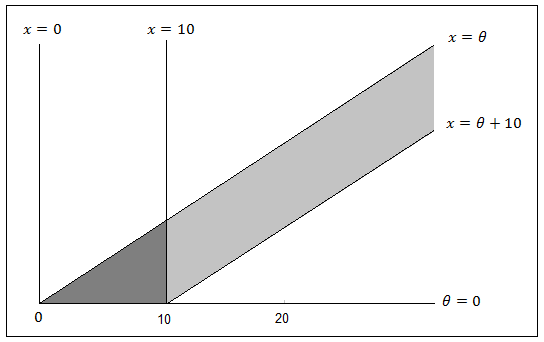
\includegraphics{Figures/Fig3Exer.png}
\caption{}
\end{figure}

\[f_{X}\left( x \right) = \left\{ \begin{matrix}
\int_{0}^{x}{\frac{1}{50}e^{- \frac{\theta}{5}}d\theta = \frac{1}{10}\left( 1 - e^{- \frac{x}{5}} \right)} & 0 \leq x \leq 10, \\
\int_{x - 10}^{x}{\frac{1}{50}e^{- \frac{\theta}{5}} d\theta} = \frac{1}{10}\left( e^{- \frac{\left( x - 10 \right)}{5}} - e^{- \frac{x}{5}} \right) & 10 < x < \infty. \\
\end{matrix} \right.\ \]

\section{Coverage Modifications}\label{coverage-modifications}

In this section we evaluate the impacts of coverage modifications: a)
deductibles, b) policy limit, c) coinsurance and inflation on insurer's
costs.

\subsection{Policy Deductibles}\label{PolicyDeduct}

Under an ordinary deductible policy, the insured (policyholder) agrees
to cover a fixed amount of an insurance claim before the insurer starts
to pay. This fixed expense paid out of pocket is called the deductible
and often denoted by \(d\). The insurer is responsible for covering the
loss \(X\) less the deductible \(d\). Depending on the agreement, the
deductible may apply to each covered loss or to a defined benefit period
(month, year, etc.)

Deductibles eliminate a large number of small claims, reduce costs of
handling and processing these claims, reduce premiums for the
policyholders and reduce moral hazard. Moral hazard occurs when the
insured takes more risks, increasing the chances of loss due to perils
insured against, knowing that the insurer will incur the cost (e.g.~a
policyholder with collision insurance may be encouraged to drive
recklessly). The larger the deductible, the less the insured pays in
premiums for an insurance policy.

Let \(X\) denote the loss incurred to the insured and \(Y\) denote the
amount of paid claim by the insurer. Speaking of the benefit paid to the
policyholder, we differentiate between two variables: The payment per
loss and the payment per payment. The payment per loss variable, denoted
by \(Y^{L}\), includes losses for which a payment is made as well as
losses less than the deductible and hence is defined as
\[Y^{L} = \left( X - d \right)_{+} 
= \left\{ \begin{array}{cc}
0 & X < d, \\
X - d & X > d  
\end{array} \right. .\] \(Y^{L}\) is often referred to as left censored
and shifted variable because the values below \(d\) are not ignored and
all losses are shifted by a value \(d\).

On the other hand, the payment per payment variable, denoted by
\(Y^{P}\), is not defined when there is no payment and only includes
losses for which a payment is made. The variable is defined as
\[Y^{P} = \left\{ \begin{matrix}
\text{Undefined} & X \le d \\
X - d & X > d 
\end{matrix} \right. \] \(Y^{P}\) is often referred to as left truncated
and shifted variable or excess loss variable because the claims smaller
than \(d\) are not reported and values above \(d\) are shifted by \(d\).

Even when the distribution of \(X\) is continuous, the distribution of
\(Y^{L}\) is partly discrete and partly continuous. The discrete part of
the distribution is concentrated at \(Y = 0\) (when \(X \leq d\)) and
the continuous part is spread over the interval \(Y > 0\) (when
\(X > d\)). For the discrete part, the probability that no payment is
made is the probability that losses fall below the deductible; that is,
\[\Pr\left( Y^{L} = 0 \right) = \Pr\left( X \leq d \right) = F_{X}\left( d \right).\]
Using the transformation \(Y^{L} = X - d\) for the continuous part of
the distribution, we can find the probability density function of
\(Y^{L}\) given by \[f_{Y^{L}}\left( y \right) = \left\{ \begin{matrix}
F_{X}\left( d \right) & y = 0, \\
f_{X}\left( y + d \right) & y > 0 
\end{matrix} \right. \]

We can see that the payment per payment variable is the payment per loss
variable conditioned on the loss exceeding the deductible; that is,
\(Y^{P} = \left. \ Y^{L} \right|X > d\). Hence, the probability density
function of \(Y^{P}\) is given by
\[f_{Y^{P}}\left( y \right) = \frac{f_{X}\left( y + d \right)}{1 - F_{X}\left( d \right)},\]
for \(y > 0\). Accordingly, the distribution functions of \(Y^{L}\)and
\(Y^{P}\) are given by
\[F_{Y^{L}}\left( y \right) = \left\{ \begin{matrix}
F_{X}\left( d \right) & y = 0, \\
F_{X}\left( y + d \right) & y > 0. \\
\end{matrix} \right.\ \] and
\[F_{Y^{P}}\left( y \right) = \frac{F_{X}\left( y + d \right) - F_{X}\left( d \right)}{1 - F_{X}\left( d \right)},\]
for \(y > 0\), respectively.

The raw moments of \(Y^{L}\) and \(Y^{P}\) can be found directly using
the probability density function of \(X\) as follows
\[E\left\lbrack \left( Y^{L} \right)^{k} \right\rbrack = \int_{d}^{\infty}\left( x - d \right)^{k}f_{X}\left( x \right)dx ,\]
and
\[E\left\lbrack \left( Y^{P} \right)^{k} \right\rbrack = \frac{\int_{d}^{\infty}\left( x - d \right)^{k}f_{X}\left( x \right) dx }{{1 - F}_{X}\left( d \right)} = \frac{E\left\lbrack \left( Y^{L} \right)^{k} \right\rbrack}{{1 - F}_{X}\left( d \right)},\]
respectively.

We have seen that the deductible \(d\) imposed on an insurance policy is
the amount of loss that has to be paid out of pocket before the insurer
makes any payment. The deductible \(d\) imposed on an insurance policy
reduces the insurer's payment. The loss elimination ratio (\emph{LER})
is the percentage decrease in the expected payment of the insurer as a
result of imposing the deductible. \emph{LER} is defined as
\[LER = \frac{E\left( X \right) - E\left( Y^{L} \right)}{E\left( X \right)}.\]

A little less common type of policy deductible is the franchise
deductible. The Franchise deductible will apply to the policy in the
same way as ordinary deductible except that when the loss exceeds the
deductible \(d\), the full loss is covered by the insurer. The payment
per loss and payment per payment variables are defined as
\[Y^{L} = \left\{ \begin{matrix}
0 & X \leq d, \\
X & X > d, \\
\end{matrix} \right.\ \] and \[Y^{P} = \left\{ \begin{matrix}
\text{Undefined} & X \leq d, \\
X & X > d, \\
\end{matrix} \right.\ \] respectively.

Example 3.15 (SOA) A claim severity distribution is exponential with
mean 1000. An insurance company will pay the amount of each claim in
excess of a deductible of 100. Calculate the variance of the amount paid
by the insurance company for one claim, including the possibility that
the amount paid is 0.

Solution

Let \(Y^{L}\) denote the amount paid by the insurance company for one
claim. \[Y^{L} = \left( X - 100 \right)_{+} = \left\{ \begin{matrix}
0 & X \leq 100, \\
X - 100 & X > 100. \\
\end{matrix} \right.\ \] The first and second moments of \(Y^{L}\) are
\[E\left( Y^{L} \right) = \int_{100}^{\infty}\left( x - 100 \right)f_{X}\left( x \right)dx \\
= {\int_{100}^{\infty}{S_{X}\left( x \right)}dx = 1000e}^{- \frac{100}{1000}},\]
and
\[E\left\lbrack \left( Y^{L} \right)^{2} \right\rbrack = \int_{100}^{\infty}\left( x - 100 \right)^{2}f_{X}\left( x \right)dx \\
= 2 \times 1000^{2}e^{- \frac{100}{1000}}.\]
\[Var\left( Y^{L} \right) = \left( 2 \times 1000^{2}e^{- \frac{100}{1000}} \right) - \left( {1000e}^{- \frac{100}{1000}} \right)^{2} = 990,944.\]

The solution can be simplified if we make use of the relationship
between \(X\) and \(Y^{P}\). If \(X\) is exponentially distributed with
mean 1000, then \(Y^{P}\) is also exponentially distributed with the
same mean. Hence, \(E\left( Y^{P} \right)\)=1000 and
\[E\left\lbrack \left( Y^{P} \right)^{2} \right\rbrack = 2 \times 1000^{2}.\]
Using the relationship between \(Y^{L}\) and \(Y^{P}\) we find
\[E\left( Y^{L} \right) = \ E\left( Y^{P} \right)S_{X}\left( 100 \right){= 1000e}^{- \frac{100}{1000}}\]

\[E\left\lbrack \left( Y^{L} \right)^{2} \right\rbrack = E\left\lbrack \left( Y^{P} \right)^{2} \right\rbrack S_{X}\left( 100 \right) = 2 \times 1000^{2}e^{- \frac{100}{1000}}.\]

Example 3.16 (SOA) For an insurance:

Losses have a density function
\[f_{X}\left( x \right) = \left\{ \begin{matrix}
    0.02x & 0 < x  < 10, \\
    0 & \text{elsewhere.} \\
    \end{matrix} \right. \]

The insurance has an ordinary deductible of 4 per loss.

\(Y^{P}\) is the claim payment per payment random variable.

Calculate \(E\left( Y^{P} \right)\).

Solution

\[Y^{P} = \left\{ \begin{matrix}
\text{Undefined} & X \leq 4, \\
X - 4 & X > 4. \\
\end{matrix} \right.\ \]

\(E\left( Y^{P} \right) = \frac{\int_{4}^{10}\left( x - 4 \right)0.02xdx}{{1 - F}_{X}\left( 4 \right)} = \frac{2.88}{0.84} = 3.43\).

Example 3.17 (SOA) You are given:

Losses follow an exponential distribution with the same mean in all
years.

The loss elimination ratio this year is 70\%.

The ordinary deductible for the coming year is 4/3 of the current
deductible.

Compute the loss elimination ratio for the coming year.

Solution

The \emph{LER} for the current year is
\[\frac{E\left( X \right) - E\left( Y^{L} \right)}{E\left( X \right)} = \frac{\theta - \theta e^{- d / \theta}}{\theta} = 1 - e^{- d / \theta} = 0.7.\]
Then, \(e^{- d / \theta} = 0.3\).

The \emph{LER} for the coming year is
\[ \frac{\theta - \theta e^{- \frac{\left( \frac{4}{3}d \right)}{\theta}}}{\theta} = 1 - e^{- \frac{\left( \frac{4}{3} d \right)}{\theta}} = 1 - \left( e^{-d /\theta} \right)^{4/3} = 1 - {0.3}^{4/3} = 0.8 .\]

\subsection{Policy Limits}\label{PolicyLimits}

Under a limited policy, the insurer is responsible for covering the
actual loss \(X\) up to the limit of its coverage. This fixed limit of
coverage is called the policy limit and often denoted by \(u\). If the
loss exceeds the policy limit, the difference \(X - u\) has to be paid
by the policyholder. While a higher policy limit means a higher payout
to the insured, it is associated with a higher premium.

Let \(X\) denote the loss incurred to the insured and \(Y\) denote the
amount of paid claim by the insurer. Then \(Y\) is defined as
\[Y = X \land u = \left\{ \begin{matrix}
X & X \leq u, \\
u & X > u. \\
\end{matrix} \right.\ \] It can be seen that the distinction between
\(Y^{L}\) and \(Y^{P}\) is not needed under limited policy as the
insurer will always make a payment.

Even when the distribution of \(X\) is continuous, the distribution of
\(Y\) is partly discrete and partly continuous. The discrete part of the
distribution is concentrated at \(Y = u\) (when \(X > u\)), while the
continuous part is spread over the interval \(Y < u\) (when
\(X \leq u\)). For the discrete part, the probability that the benefit
paid is \(u\), is the probability that the loss exceeds the policy limit
\(u\); that is,
\[\Pr \left( Y = u \right) = \Pr \left( X > u \right) = {1 - F}_{X}\left( u \right).\]
For the continuous part of the distribution \(Y = X\), hence the
probability density function of \(Y\) is given by
\[f_{Y}\left( y \right) = \left\{ \begin{matrix}
f_{X}\left( y \right) & 0 < y < u, \\
1 - F_{X}\left( u \right) & y = u. \\
\end{matrix} \right.\ \] Accordingly, the distribution function of \(Y\)
is given by \[F_{Y}\left( y \right) = \left\{ \begin{matrix}
F_{X}\left( x \right) & 0 < y < u, \\
1 & y \geq u. \\
\end{matrix} \right.\ \] The raw moments of \(Y\) can be found directly
using the probability density function of \(X\) as follows
\[E\left( Y^{k} \right) = E\left\lbrack \left( X \land u \right)^{k} \right\rbrack = \int_{0}^{u}x^{k}f_{X}\left( x \right)dx + \int_{u}^{\infty}{u^{k}f_{X}\left( x \right)} dx \\ \int_{0}^{u}x^{k}f_{X}\left( x \right)dx + u^{k}\left\lbrack {1 - F}_{X}\left( u \right) \right\rbrack dx.\]

Example 3.18 (SOA) Under a group insurance policy, an insurer agrees to
pay 100\% of the medical bills incurred during the year by employees of
a small company, up to a maximum total of one million dollars. The total
amount of bills incurred, \(X\), has probability density function
\[f_{X}\left( x \right) = \left\{ \begin{matrix}
\frac{x\left( 4 - x \right)}{9} & 0 < x < 3, \\
0 & \text{elsewhere.} \\
\end{matrix} \right.\ \] where \(x\) is measured in millions. Calculate
the total amount, in millions of dollars, the insurer would expect to
pay under this policy. Solution

\[Y = X \land 1 = \left\{ \begin{matrix}
X & X \leq 1, \\
1 & X > 1. \\
\end{matrix} \right.\ \]

\(E\left( Y \right) = E\left( X \land 1 \right) = \int_{0}^{1}\frac{x^{2}(4 - x)}{9}dx + \int_{1}^{3}\frac{x\left( 4 - x \right)}{9}dx = 0.935\).

\subsection{Coinsurance}\label{coinsurance}

As we have seen in Section \ref{PolicyDeduct}, the amount of loss
retained by the policyholder can be losses up to the deductible \(d\).
The retained loss can also be a percentage of the claim. The percentage
\(\alpha\), often referred to as the coinsurance factor, is the
percentage of claim the insurance company is required to cover. If the
policy is subject to an ordinary deductible and policy limit,
coinsurance refers to the percentage of claim the insurer is required to
cover, after imposing the ordinary deductible and policy limit. The
payment per loss variable, \(Y^{L}\), is defined as
\[Y^{L} = \left\{ \begin{matrix}
0 & X \leq d, \\
\alpha\left( X - d \right) & d <  X \leq u, \\
\alpha\left( u - d \right) & X > u. \\
\end{matrix} \right.\ \] The policy limit (the maximum amount paid by
the insurer) in this case is \(\alpha\left( u - d \right)\), while \(u\)
is the maximum covered loss.

The \(k\)-th moment of \(Y^{L}\) is given by
\[E\left\lbrack \left( Y^{L} \right)^{k} \right\rbrack = \int_{d}^{u}\left\lbrack \alpha\left( x - d \right) \right\rbrack^{k}f_{X}\left( x \right)dx + \int_{u}^{\infty}\left\lbrack \alpha\left( u - d \right) \right\rbrack^{k}f_{X}\left( x \right) dx .\]

A growth factor \(\left( 1 + r \right)\) may be applied to \(X\)
resulting in an inflated loss random variable \(\left( 1 + r \right)X\)
(the prespecified \emph{d} and \emph{u} remain unchanged). The resulting
per loss variable can be written as \[Y^{L} = \left\{ \begin{matrix}
0 & X \leq \frac{d}{1 + r}, \\
\alpha\left\lbrack \left( 1 + r \right)X - d \right\rbrack & \frac{d}{1 + r} <  X \leq \frac{u}{1 + r}, \\
\alpha\left( u - d \right) & X > \frac{u}{1 + r}. \\
\end{matrix} \right.\ \] The first and second moments of \(Y^{L}\) can
be expressed as
\[E\left( Y^{L} \right) = \alpha\left( 1 + r \right)\left\lbrack E\left( X \land \frac{u}{1 + r} \right) - E\left( X \land \frac{d}{1 + r} \right) \right\rbrack,\]
and \[E\left\lbrack \left( Y^{L} \right)^{2} 
\right\rbrack = \alpha^{2}\left( 1 + r \right)^{2}  \left\{ E\left\lbrack \left( X \land \frac{u}{1 + r} \right)^{2} \right\rbrack - E\left\lbrack \left( X \land \frac{d}{1 + r} \right)^{2} \right\rbrack  \right. \\
\left. \ \ \ \ \ - 2\left( \frac{d}{1 + r} \right)\left\lbrack E\left( X \land \frac{u}{1 + r} \right) - E\left( X \land \frac{d}{1 + r} \right) \right\rbrack \right\} ,\]
respectively.

The formulae given for the first and second moments of \(Y^{L}\) are
general. Under full coverage, \(\alpha = 1\), \(r = 0\), \(u = \infty\),
\(d = 0\) and \(E\left( Y^{L} \right)\) reduces to
\(E\left( X \right)\). If only an ordinary deductible is imposed,
\(\alpha = 1\), \(r = 0\), \(u = \infty\) and \(E\left( Y^{L} \right)\)
reduces to \(E\left( X \right) - E\left( X \land d \right)\). If only a
policy limit is imposed \(\alpha = 1\), \(r = 0\), \(d = 0\) and
\(E\left( Y^{L} \right)\) reduces to \(E\left( X \land u \right)\).

Example 3.19 (SOA) The ground up loss random variable for a health
insurance policy in 2006 is modeled with \emph{X}, an exponential
distribution with mean 1000. An insurance policy pays the loss above an
ordinary deductible of 100, with a maximum annual payment of 500. The
ground up loss random variable is expected to be 5\% larger in 2007, but
the insurance in 2007 has the same deductible and maximum payment as in
2006. Find the percentage increase in the expected cost per payment from
2006 to 2007. Solution

\[Y_{2006}^{L} = \left\{ \begin{matrix}
0 & X \leq 100, \\
X - 100 & 100 <  X \leq 600, \\
500 & X > 600. \\
\end{matrix} \right.\ \]

\[Y_{2007}^{L} = \left\{ \begin{matrix}
0 & X \leq 95.24, \\
1.05X - 100 & 95.24 <  X \leq 571.43, \\
500 & X > 571.43. \\
\end{matrix} \right.\ \]

\[E\left( Y_{2006}^{L} \right) = E\left( X \land 600 \right) - E\left( X \land 100 \right) = 1000\left( {1 - e}^{- \frac{600}{1000}} \right) - 1000\left( {1 - e}^{- \frac{100}{1000}} \right)\]

\(= 356.026\).

\[E\left( Y_{2007}^{L} \right) = 1.05\left\lbrack E\left( X \land 571.43 \right) - E\left( X \land 95.24 \right) \right\rbrack\]

\(= 1.05\left\lbrack 1000\left( {1 - e}^{- \frac{571.43}{1000}} \right) - 1000\left( {1 - e}^{- \frac{95.24}{1000}} \right) \right\rbrack\)

\(\mathbf{=}361.659\).

\(E\left( Y_{2006}^{P} \right) = \frac{356.026}{e^{- \frac{100}{1000}} = 393.469}\).

\(E\left( Y_{2007}^{P} \right) = \frac{361.659}{e^{- \frac{95.24}{1000}} = 397.797}\).

There is an increase of 1.1\% from 2006 to 2007.

\subsection{Reinsurance}\label{reinsurance}

In Section \ref{PolicyDeduct} we introduced the policy deductible, which
is a contractual arrangement under which an insured transfers part of
the risk by securing coverage from an insurer in return for an insurance
premium. Under that policy, when the loss exceeds the deductible, the
insurer is not required to pay until the insured has paid the fixed
deductible. We now introduce reinsurance, a mechanism of insurance for
insurance companies. Reinsurance is a contractual arrangement under
which an insurer transfers part of the underlying insured risk by
securing coverage from another insurer (referred to as a reinsurer) in
return for a reinsurance premium. Although reinsurance involves a
relationship between three parties: the original insured, the insurer
(often referred to as cedent or cedant) and the reinsurer, the parties
of the reinsurance agreement are only the primary insurer and the
reinsurer. There is no contractual agreement between the original
insured and the reinsurer. The reinsurer is not required to pay under
the reinsurance contract until the insurer has paid a loss to its
original insured. The amount retained by the primary insurer in the
reinsurance agreement (the reinsurance deductible) is called retention.

Reinsurance arrangements allow insurers with limited financial resources
to increase the capacity to write insurance and meet client requests for
larger insurance coverage while reducing the impact of potential losses
and protecting the insurance company against catastrophic losses.
Reinsurance also allows the primary insurer to benefit from underwriting
skills, expertize and proficient complex claim file handling of the
larger reinsurance companies.

Example 3.20 (SOA) In 2005 a risk has a two-parameter Pareto
distribution with \(\alpha = 2\) and \(\theta = 3000\). In 2006 losses
inflate by 20\%. Insurance on the risk has a deductible of 600 in each
year. \(P_{i}\), the premium in year \(i\), equals 1.2 times expected
claims. The risk is reinsured with a deductible that stays the same in
each year. \(R_{i}\), the reinsurance premium in year \(i\), equals 1.1
times the expected reinsured claims.
\(\frac{R_{2005}}{P_{2005} = 0.55}\). Calculate
\(\frac{R_{2006}}{P_{2006}}\). Solution

Let us use the following notation:

\(X_{i}:\) The risk in year \(i\)

\(Y_{i}:\) The insured claim in year \(i\)

\(P_{i}:\) The insurance premium in year \(i\)

\(Y_{i}^{R}:\) The reinsured claim in year \(i\)

\(R_{i}:\) The reinsurance premium in year \(i\)

\(d:\) The insurance deductible in year \(i\) (the insurance deductible
is fixed each year, equal to 600)

\(d^{R}:\) The reinsurance deductible or retention in year \(i\) (the
reinsurance deductible is fixed each year, but unknown) where
\(i = 2005,\ 2006\)

\[Y_{i} = \left\{ \begin{matrix}
0 & X_{i} \leq 600 \\
X_{i} - 600 & X_{i} > 600 \\
\end{matrix} \right.\ \] where \(i = 2005,\ 2006\)

\[X_{2005}\sim Pa\left( 2,3000 \right)\]

\[E\left( Y_{2005} \right) = E\left( X_{2005} - 600 \right)_{+} = E\left( X_{2005} \right) - E\left( X_{2005} \land 600 \right)\]

\(= 3000 - 3000\left( 1 - \frac{3000}{3600} \right) = 2500\)

\[P_{2005} = 1.2E\left( Y_{2005} \right) = 3000\]

Since \(X_{2006} = 1.2X_{2005}\) and Pareto is a scale distribution with
scale parameter \(\theta\), then
\(X_{2006}\sim Pa\left( 2,3600 \right)\)

\[E\left( Y_{2006} \right) = E\left( X_{2006} - 600 \right)_{+} = E\left( X_{2006} \right) - E\left( X_{2006} \land 600 \right)\]

\(= 3600 - 3600\left( 1 - \frac{3600}{4200} \right) = 3085.714\)

\[P_{2006} = 1.2E\left( Y_{2006} \right) = 3702.857\]

\[Y_{i}^{R} = \left\{ \begin{matrix}
0 & X_{i} - 600 \leq d^{R} \\
X_{i} - 600 - d^{R} & X_{i} - 600 > d^{R} \\
\end{matrix} \right.\ \]

Since \(\frac{R_{2005}}{P_{2005}} = 0.55\), then
\(R_{2005} = 3000 \times 0.55 = 1650\)

Since \(R_{2005} = 1.1E\left( Y_{2005}^{R} \right)\), then
\(E\left( Y_{2005}^{R} \right) = \frac{1650}{1.1} = 1500\)

\[E\left( Y_{2005}^{R} \right) = E\left( X_{2005} - 600 - d^{R} \right)_{+} = E\left( X_{2005} \right) - E\left( X_{2005} \land \left( 600 + d^{R} \right) \right)\]

\(= 3000 - 3000\left( 1 - \frac{3000}{3600 + d^{R}} \right) = 1500 \Rightarrow d^{R} = 2400\)

\[E\left( Y_{2006}^{R} \right) = E\left( X_{2006} - 600 - d^{R} \right)_{+} = E\left( X_{2006} - 3000 \right)_{+} = E\left( X_{2006} \right) - E\left( X_{2006} \land 3000 \right)\]

\(= 3600 - 3600\left( 1 - \frac{3600}{6600} \right) = 1963.636\)

\[R_{2006} = 1.1E\left( Y_{2006}^{R} \right) = 1.1 \times 1963.636 = 2160\]

Therefore \(\frac{R_{2006}}{P_{2006}} = \frac{2160}{3702.857} = 0.583\)

\section{Maximum Likelihood
Estimation}\label{maximum-likelihood-estimation}

In this section we estimate statistical parameters using the method of
maximum likelihood. Maximum likelihood estimates in the presence of
grouping, truncation or censoring are calculated.

\subsection{Maximum Likelihood Estimators for Complete
Data}\label{maximum-likelihood-estimators-for-complete-data}

Pricing of insurance premiums and estimation of claim reserving are
among many actuarial problems that involve modeling the severity of loss
(claim size). The principles for using maximum likelihood to estimate
model parameters were introduced in Chapter \textbf{xxx}. In this
section, we present a few examples to illustrate how actuaries fit a
parametric distribution model to a set of claim data using maximum
likelihood. In these examples we derive the asymptotic variance of
maximum-likelihood estimators of the model parameters. We use the delta
method to derive the asymptotic variances of functions of these
parameters.

Example 3.21 Consider a random sample of claim amounts: 8,000 10,000
12,000 15,000. You assume that claim amounts follow an inverse
exponential distribution, with parameter \(\theta\).

Calculate the maximum likelihood estimator for \(\theta\).

Approximate the variance of the maximum likelihood estimator.

Determine an approximate 95\% confidence interval for \(\theta\).

Determine an approximate 95\% confidence interval for
\(\Pr \left( X \leq 9,000 \right).\)

Solution

The probability density function is
\[f_{X}\left( x \right) = \frac{\theta e^{- \frac{\theta}{x}}}{x^{2}}, \]
where \(x > 0\). The likelihood function, \(L\left( \theta \right)\),
can be viewed as the probability of the observed data, written as a
function of the model's parameter \(\theta\)
\[L\left( \theta \right) = \prod_{i = 1}^{4}{f_{X_{i}}\left( x_{i} \right)} = \frac{\theta^{4}e^{- \theta\sum_{i = 1}^{4}\frac{1}{x_{i}}}}{\prod_{i = 1}^{4}x_{i}^{2}}.\]

The loglikelihood function, \(\ln L \left( \theta \right)\), is the sum
of the individual logarithms.
\[\ln L \left( \theta \right) = 4ln\theta - \theta\sum_{i = 1}^{4}\frac{1}{x_{i}} - 2\sum_{i = 1}^{4}\ln x_{i} .\]

\[\frac{d \ln L \left( \theta \right)}{d \theta} = \frac{4}{\theta} - \sum_{i = 1}^{4}\frac{1}{x_{i}}.\]
The maximum likelihood estimator of \(\theta\), denoted by
\(\hat{\theta}\), is the solution to the equation
\[\frac{4}{\hat{\theta}} - \sum_{i = 1}^{4}{\frac{1}{x_{i}} = 0}.\]
Thus,
\(\hat{\theta} = \frac{4}{\sum_{i = 1}^{4}\frac{1}{x_{i}}} = 10,667\)

The second derivative of \(\ln L \left( \theta \right)\) is given by
\[\frac{d^{2}\ln L\left( \theta \right)}{d\theta^{2}} = \frac{- 4}{\theta^{2}}.\]
Evaluating the second derivative of the loglikelihood function at
\(\hat{\theta} = 10,667\) gives a negative value, indicating
\(\hat{\theta}\) as the value that maximizes the loglikelihood function.

Taking reciprocal of negative expectation of the second derivative of
\(\ln L \left( \theta \right)\), we obtain an estimate of the variance
of \(\hat{\theta}\)
\(\widehat{Var}\left( \hat{\theta} \right) = \left. \ \left\lbrack E\left( \frac{d^{2}\ln L \left( \theta \right)}{d\theta^{2}} \right) \right\rbrack^{- 1} \right|_{\theta = \hat{\theta}} = \frac{{\hat{\theta}}^{2}}{4} = 28,446,222\).

It should be noted that as the sample size \(n \rightarrow \infty\), the
distribution of the maximum likelihood estimator \(\hat{\theta}\)
converges to a normal distribution with mean \(\theta\) and variance
\(\hat{V}\left( \hat{\theta} \right)\). The approximate confidence
interval in this example is based on the assumption of normality,
despite the small sample size, only for the purpose of illustration.

The 95\% confidence interval for \(\theta\) is given by
\[10,667 \pm 1.96\sqrt{28,446,222} = \left( 213.34,\ 21,120.66 \right).\]
The distribution function of \(X\) is
\(F\left( x \right) = 1 - e^{- \frac{x}{\theta}}\). Then, the maximum
likelihood estimate of
\(g\left( \theta \right) = F\left( 9,000 \right)\) is
\[g\left( \hat{\theta} \right) = 1 - e^{- \frac{9,000}{10,667}} = 0.57.\]
We use the delta method to approximate the variance of
\(g\left( \hat{\theta} \right)\).
\[\frac{\text{dg}\left( \theta \right)}{d \theta} = {- \frac{9,000}{\theta^{2}}e}^{- \frac{9,000}{\theta}}.\]

\(\widehat{Var}\left\lbrack g\left( \hat{\theta} \right) \right\rbrack = \left( - {\frac{9,000}{{\hat{\theta}}^{2}}e}^{- \frac{9,000}{\hat{\theta}}} \right)^{2}\hat{V}\left( \hat{\theta} \right) = 0.0329\).

The 95\% confidence interval for \(F\left( 9,000 \right)\) is given by
\[0.57 \pm 1.96\sqrt{0.0329} = \left( 0.214,\ 0.926 \right).\]

Example 3.22 A random sample of size 6 is from a lognormal distribution
with parameters \(\mu\) and \(\sigma\). The sample values are 200,
3,000, 8,000, 60,000, 60,000, 160,000.

Calculate the maximum likelihood estimator for \(\mu\) and \(\sigma\).

Estimate the covariance matrix of the maximum likelihood estimator.

Determine approximate 95\% confidence intervals for \(\mu\) and
\(\sigma\).

Determine an approximate 95\% confidence interval for the mean of the
lognormal distribution.

Solution

The probability density function is
\[f_{X}\left( x \right) = \frac{1}{x \sigma \sqrt{2\pi}}\exp - \frac{1}{2}\left( \frac{\ln x - \mu}{\sigma} \right)^{2},\]
where \(x > 0\). The likelihood function,
\(L\left( \mu,\sigma \right)\), is the product of the pdf for each data
point.
\[L\left( \mu,\sigma \right) = \prod_{i = 1}^{6}{f_{X_{i}}\left( x_{i} \right)} = \frac{1}{\sigma^{6}\left( 2\pi \right)^{3}\prod_{i = 1}^{6}x_{i}}exp - \frac{1}{2}\sum_{i = 1}^{6}\left( \frac{\ln x_{i} - \mu}{\sigma} \right)^{2}.\]
The loglikelihood function, \(\ln L \left( \mu,\sigma \right)\), is the
sum of the individual logarithms.
\[\ln \left( \mu,\sigma \right) = - 6ln\sigma - 3ln\left( 2\pi \right) - \sum_{i = 1}^{6}\ln x_{i} - \frac{1}{2}\sum_{i = 1}^{6}\left( \frac{\ln x_{i} - \mu}{\sigma} \right)^{2}.\]
The first partial derivatives are
\[\frac{\partial lnL\left( \mu,\sigma \right)}{\partial\mu} = \frac{1}{\sigma^{2}}\sum_{i = 1}^{6}\left( \ln x_{i} - \mu \right).\]
\[\frac{\partial lnL\left( \mu,\sigma \right)}{\partial\sigma} = \frac{- 6}{\sigma} + \frac{1}{\sigma^{3}}\sum_{i = 1}^{6}\left( \ln x_{i} - \mu \right)^{2}.\]
The maximum likelihood estimators of \(\mu\) and \(\sigma\), denoted by
\(\hat{\mu}\) and \(\hat{\sigma}\), are the solutions to the equations
\[\frac{1}{{\hat{\sigma}}^{2}}\sum_{i = 1}^{6}\left( lnx_{i} - \hat{\mu} \right) = 0.\]
\[\frac{- 6}{\hat{\sigma}} + \frac{1}{{\hat{\sigma}}^{3}}\sum_{i = 1}^{6}\left( \ln x_{i} - \hat{\mu} \right)^{2} = 0.\]
These yield the estimates

\(\hat{\mu} = \frac{\sum_{i = 1}^{6}{\ln x_{i}}}{6} = 9.38\) and
\({\hat{\sigma}}^{2} = \frac{\sum_{i = 1}^{6}\left( \ln x_{i} - \hat{\mu} \right)^{2}}{6} = 5.12\).

The second partial derivatives are

\(\frac{\partial^{2}\text{lnL}\left( \mu,\sigma \right)}{\partial\mu^{2}} = \frac{- 6}{\sigma^{2}}\),
\(\frac{\partial^{2}\text{lnL}\left( \mu,\sigma \right)}{\partial\mu\partial\sigma} = \frac{- 2}{\sigma^{3}}\sum_{i = 1}^{6}\left( \ln x_{i} - \mu \right)\)
and
\(\frac{\partial^{2}\text{lnL}\left( \mu,\sigma \right)}{\partial\sigma^{2}} = \frac{6}{\sigma^{2}} - \frac{3}{\sigma^{4}}\sum_{i = 1}^{6}\left( \ln x_{i} - \mu \right)^{2}\).

To derive the covariance matrix of the mle we need to find the
expectations of the second derivatives. Since the random variable \(X\)
is from a lognormal distribution with parameters \(\mu\) and \(\sigma\),
then \(\text{lnX}\) is normally distributed with mean \(\mu\) and
variance \(\sigma^{2}\).

\(E\left( \frac{\partial^{2}\text{lnL}\left( \mu,\sigma \right)}{\partial\mu^{2}} \right) = E\left( \frac{- 6}{\sigma^{2}} \right) = \frac{- 6}{\sigma^{2}}\),

\(E\left( \frac{\partial^{2}\text{lnL}\left( \mu,\sigma \right)}{\partial\mu\partial\sigma} \right) = \frac{- 2}{\sigma^{3}}\sum_{i = 1}^{6}{E\left( \ln x_{i} - \mu \right)} = \frac{- 2}{\sigma^{3}}\sum_{i = 1}^{6}\left\lbrack E\left( \ln x_{i} \right) - \mu \right\rbrack\)=\(\frac{- 2}{\sigma^{3}}\sum_{i = 1}^{6}\left( \mu - \mu \right) = 0\),

and

\(E\left( \frac{\partial^{2}\text{lnL}\left( \mu,\sigma \right)}{\partial\sigma^{2}} \right) = \frac{6}{\sigma^{2}} - \frac{3}{\sigma^{4}}\sum_{i = 1}^{6}{E\left( \ln x_{i} - \mu \right)}^{2} = \frac{6}{\sigma^{2}} - \frac{3}{\sigma^{4}}\sum_{i = 1}^{6}{V\left( \ln x_{i} \right) = \frac{6}{\sigma^{2}} - \frac{3}{\sigma^{4}}\sum_{i = 1}^{6}{\sigma^{2} = \frac{- 12}{\sigma^{2}}}}\).

Using the negatives of these expectations we obtain the Fisher
information matrix \[\begin{bmatrix}
\frac{6}{\sigma^{2}} & 0 \\
0 & \frac{12}{\sigma^{2}} \\
\end{bmatrix}\].

The covariance matrix, \(\Sigma\), is the inverse of the Fisher
information matrix \[\Sigma = \begin{bmatrix}
\frac{\sigma^{2}}{6} & 0 \\
0 & \frac{\sigma^{2}}{12} \\
\end{bmatrix}\].

The estimated matrix is given by \[\hat{\Sigma} = \begin{bmatrix}
0.8533 & 0 \\
0 & 0.4267 \\
\end{bmatrix}\].

The 95\% confidence interval for \(\mu\) is given by
\(9.38 \pm 1.96\sqrt{0.8533} = \left( 7.57,\ 11.19 \right)\).

The 95\% confidence interval for \(\sigma^{2}\) is given by
\(5.12 \pm 1.96\sqrt{0.4267} = \left( 3.84,\ 6.40 \right)\).

The mean of \emph{X} is
\(\exp\left( \mu + \frac{\sigma^{2}}{2} \right)\). Then, the maximum
likelihood estimate of
\[g\left( \mu,\sigma \right) = \exp\left( \mu + \frac{\sigma^{2}}{2} \right)\]
is
\[g\left( \hat{\mu},\hat{\sigma} \right) = \exp\left( \hat{\mu} + \frac{{\hat{\sigma}}^{2}}{2} \right) = 153,277.\]

We use the delta method to approximate the variance of the mle
\(g\left( \hat{\mu},\hat{\sigma} \right)\).

\(\frac{\partial g\left( \mu,\sigma \right)}{\partial\mu} = exp\left( \mu + \frac{\sigma^{2}}{2} \right)\)
and
\(\frac{\partial g\left( \mu,\sigma \right)}{\partial\sigma} = \sigma exp\left( \mu + \frac{\sigma^{2}}{2} \right)\).

Using the delta method, the approximate variance of
\(g\left( \hat{\mu},\hat{\sigma} \right)\) is given by

\[\left. \ \hat{V}\left( g\left( \hat{\mu},\hat{\sigma} \right) \right) = \begin{bmatrix}
\frac{\partial g\left( \mu,\sigma \right)}{\partial\mu} & \frac{\partial g\left( \mu,\sigma \right)}{\partial\sigma} \\
\end{bmatrix}\Sigma\begin{bmatrix}
\frac{\partial g\left( \mu,\sigma \right)}{\partial\mu} \\
\frac{\partial g\left( \mu,\sigma \right)}{\partial\sigma} \\
\end{bmatrix} \right|_{\mu = \hat{\mu},\sigma = \hat{\sigma}}\]

\[= \begin{bmatrix}
153,277 & 346,826 \\
\end{bmatrix}\begin{bmatrix}
0.8533 & 0 \\
0 & 0.4267 \\
\end{bmatrix}\begin{bmatrix}
153,277 \\
346,826 \\
\end{bmatrix} =\]71,374,380,000

The 95\% confidence interval for
\(\exp\left( \mu + \frac{\sigma^{2}}{2} \right)\) is given by

\(153,277 \pm 1.96\sqrt{71,374,380,000} = \left( - 370,356,\ 676,910 \right)\).

Since the mean of the lognormal distribution cannot be negative, we
should replace the negative lower limit in the previous interval by a
zero.

\subsection{Maximum Likelihood Estimators for Grouped
Data}\label{MLEGrouped}

In the previous section we considered the maximum likelihood estimation
of continuous models from complete (individual) data. Each individual
observation is recorded, and its contribution to the likelihood function
is the density at that value. In this section we consider the problem of
obtaining maximum likelihood estimates of parameters from grouped data.
The observations are only available in grouped form, and the
contribution of each observation to the likelihood function is the
probability of falling in a specific group (interval). Let \(n_{j}\)
represent the number of observations in the interval
\(\left( \left. \ c_{j - 1},c_{j} \right\rbrack \right.\ \) The grouped
data likelihood function is thus given by
\[L\left( \theta \right) = \prod_{j = 1}^{k}\left\lbrack F\left( \left. \ c_{j} \right|\theta \right) - F\left( \left. \ c_{j - 1} \right|\theta \right) \right\rbrack^{n_{j}},\]
where \(c_{0}\) is the smallest possible observation (often set to zero)
and \(c_{k}\) is the largest possible observation (often set to
infinity).

Example 3.23 (SOA) For a group of policies, you are given that losses
follow the distribution function
\(F\left( x \right) = 1 - \frac{\theta}{x}\), for
\(\theta < x < \infty.\) Further, a sample of 20 losses resulted in the
following:

\[
{\small
\begin{matrix}\hline
\text{Interval} & \text{Number of Losses}  \\ \hline
(\theta, 10] & 9 \\
(10, 25] & 6 \\
(25, \infty) & 5  \\ \hline
\end{matrix}
}
\]

Calculate the maximum likelihood estimate of \(\theta\).

Solution

The contribution of each of the 9 observations in the first interval to
the likelihood function is the probability of \(X \leq 10\); that is,
\(\Pr\left( X \leq 10 \right) = F\left( 10 \right)\). Similarly, the
contributions of each of 6 and 5 observations in the second and third
intervals are
\(\Pr\left( 10 < X \leq 25 \right) = F\left( 25 \right) - F(10)\) and
\(P\left( X > 25 \right) = 1 - F(25)\), respectively. The likelihood
function is thus given by
\[L\left( \theta \right) = \left\lbrack F\left( 10 \right) \right\rbrack^{9}\left\lbrack F\left( 25 \right) - F(10) \right\rbrack^{6}\left\lbrack 1 - F(25) \right\rbrack^{5}\]
\[{= \left( 1 - \frac{\theta}{10} \right)}^{9}\left( \frac{\theta}{10} - \frac{\theta}{25} \right)^{6}\left( \frac{\theta}{25} \right)^{5}\]
\[{= \left( \frac{10 - \theta}{10} \right)}^{9}\left( \frac{15\theta}{250} \right)^{6}\left( \frac{\theta}{25} \right)^{5}.\]
Then,
\(\ln L \left( \theta \right) = 9ln\left( 10 - \theta \right) + 6ln\theta + 5ln\theta - 9ln10 + 6ln15 - 6ln250 - 5ln25\).
\[\frac{d \ln L \left( \theta \right)}{d \theta} = \frac{- 9}{\left( 10 - \theta \right)} + \frac{6}{\theta} + \frac{5}{\theta}.\]
The maximum likelihood estimator, \(\hat{\theta}\), is the solution to
the equation
\[\frac{- 9}{\left( 10 - \hat{\theta} \right)} + \frac{11}{\hat{\theta}} = 0\]
and \(\hat{\theta} = 5.5\).

\subsection{Maximum Likelihood Estimators for Censored
Data}\label{maximum-likelihood-estimators-for-censored-data}

Another distinguishing feature of data gathering mechanism is censoring.
While for some event of interest (losses, claims, lifetimes, etc.) the
complete data maybe available, for others only partial information is
available; information that the observation exceeds a specific value.
The limited policy introduced in Section \ref{PolicyLimits} is an
example of right censoring. Any loss greater than or equal to the policy
limit is recorded at the limit. The contribution of the censored
observation to the likelihood function is the probability of the random
variable exceeding this specific limit. Note that contributions of both
complete and censored data share the survivor function, for a complete
point this survivor function is multiplied by the hazard function, but
for a censored observation it is not.

Example 3.24 (SOA) The random variable has survival function:
\[S_{X}\left( x \right) = \frac{\theta^{4}}{\left( \theta^{2} + x^{2} \right)^{2}}.\]
Two values of \(X\) are observed to be 2 and 4. One other value exceeds
4. Calculate the maximum likelihood estimate of \(\theta\). Solution

The contributions of the two observations 2 and 4 are
\(f_{X}\left( 2 \right)\) and \(f_{X}\left( 4 \right)\) respectively.
The contribution of the third observation, which is only known to exceed
4 is \(S_{X}\left( 4 \right)\). The likelihood function is thus given by
\[L\left( \theta \right) = f_{X}\left( 2 \right)f_{X}\left( 4 \right)S_{X}\left( 4 \right).\]
The probability density function of \(X\) is given by
\[f_{X}\left( x \right) = \frac{4x\theta^{4}}{\left( \theta^{2} + x^{2} \right)^{3}}.\]
Thus,
\[L\left( \theta \right) = \frac{8\theta^{4}}{\left( \theta^{2} + 4 \right)^{3}}\frac{16\theta^{4}}{\left( \theta^{2} + 16 \right)^{3}}\frac{\theta^{4}}{\left( \theta^{2} + 16 \right)^{2}} = \\
\frac{128\theta^{12}}{\left( \theta^{2} + 4 \right)^{3}\left( \theta^{2} + 16 \right)^{5}},\]

\(\ln L\left( \theta \right) = ln128 + 12ln\theta - 3ln\left( \theta^{2} + 4 \right) - 5ln\left( \theta^{2} + 16 \right)\),

and

\(\frac{\text{dlnL}\left( \theta \right)}{d \theta} = \frac{12}{\theta} - \frac{6\theta}{\left( \theta^{2} + 4 \right)} - \frac{10\theta}{\left( \theta^{2} + 16 \right)}\).

The maximum likelihood estimator, \(\hat{\theta}\), is the solution to
the equation
\[\frac{12}{\hat{\theta}} - \frac{6\hat{\theta}}{\left( {\hat{\theta}}^{2} + 4 \right)} - \frac{10\hat{\theta}}{\left( {\hat{\theta}}^{2} + 16 \right)} = 0\]
or
\[12\left( {\hat{\theta}}^{2} + 4 \right)\left( {\hat{\theta}}^{2} + 16 \right) - 6{\hat{\theta}}^{2}\left( {\hat{\theta}}^{2} + 16 \right) - 10{\hat{\theta}}^{2}\left( {\hat{\theta}}^{2} + 4 \right) = \\
- 4{\hat{\theta}}^{4} + 104{\hat{\theta}}^{2} + 768 = 0,\] which yields
\({\hat{\theta}}^{2} = 32\) and \(\hat{\theta} = 5.7\).

\subsection{Maximum Likelihood Estimators for Truncated
Data}\label{maximum-likelihood-estimators-for-truncated-data}

This section is concerned with the maximum likelihood estimation of the
continuous distribution of the random variable \(X\) when the data is
incomplete due to truncation. If the values of \(X\) are truncated at
\(d\), then it should be noted that we would not have been aware of the
existence of these values had they not exceeded \(d\). The policy
deductible introduced in Section \ref{PolicyDeduct} is an example of
left truncation. Any loss less than or equal to the deductible is not
recorded. The contribution to the likelihood function of an observation
\(x\) truncated at \(d\) will be a conditional probability and the
\(f_{X}\left( x \right)\) will be replaced by
\(\frac{f_{X}\left( x \right)}{S_{X}\left( d \right)}\).

Example 3.25 (SOA) For the single parameter Pareto distribution with
\(\theta = 2\), maximum likelihood estimation is applied to estimate the
parameter \(\alpha\). Find the estimated mean of the ground up loss
distribution based on the maximum likelihood estimate of \(\alpha\) for
the following data set:

Ordinary policy deductible of 5, maximum covered loss of 25 (policy
limit 20)

8 insurance payment amounts: 2, 4, 5, 5, 8, 10, 12, 15

2 limit payments: 20, 20.

Solution

The contributions of the different observations can be summarized as
follows:

For the exact loss: \(f_{X}\left( x \right)\)

For censored observations: \(S_{X}\left( 25 \right)\).

For truncated observations:
\(\frac{f_{X}\left( x \right)}{S_{X}\left( 5 \right)}\).

Given that ground up losses smaller than 5 are omitted from the data
set, the contribution of all observations should be conditional on
exceeding 5. The likelihood function becomes
\[L\left( \alpha \right) = \frac{\prod_{i = 1}^{8}{f_{X}\left( x_{i} \right)}}{\left\lbrack S_{X}\left( 5 \right) \right\rbrack^{8}}\left\lbrack \frac{S_{X}\left( 25 \right)}{S_{X}\left( 5 \right)} \right\rbrack^{2}.\]
For the single parameter Pareto the probability density and distribution
functions are given by

\[f_{X}\left( x \right) = \frac{\alpha\theta^{\alpha}}{x^{\alpha + 1}} \ \ \text{and} \ \ F_{X}\left( x \right) = 1 - \left( \frac{\theta}{x} \right)^{\alpha},\]
for \(x > \theta\), respectively. Then, the likelihood and loglikelihood
functions are given by
\[L\left( \alpha \right) = \frac{\alpha^{8}}{\prod_{i = 1}^{8}x_{i}^{\alpha + 1}}\frac{5^{10\alpha}}{25^{2\alpha}},\]
\[\ln L \left( \alpha \right) = 8ln\alpha - \left( \alpha + 1 \right)\sum_{i = 1}^{8}{\ln x_{i}} + 10\alpha ln5 - 2\alpha ln25.\]

\(\frac{\text{dlnL}\left( \alpha \right)}{d \theta} = \frac{8}{\alpha} - \sum_{i = 1}^{8}{\ln x_{i}} + 10ln5 - 2ln25\).

The maximum likelihood estimator, \(\hat{\alpha}\), is the solution to
the equation
\[\frac{8}{\hat{\alpha}} - \sum_{i = 1}^{8}{\ln x_{i}} + 10ln5 - 2ln25 = 0,\]which
yields
\[\hat{\alpha} = \frac{8}{\sum_{i = 1}^{8}{\ln x_{i}} - 10ln5 + 2ln25} = \frac{8}{(ln7 + ln9 + \ldots + ln20) - 10ln5 + 2ln25} = 0.785.\]
The mean of the Pareto only exists for \(\alpha > 1\). Since
\(\hat{\alpha} = 0.785 < 1\). Then, the mean does not exist.

\section{Further Resources and
Contributors}\label{Resources-loss-severity}

In describing losses, actuaries fit appropriate parametric distribution
models for the frequency and severity of loss. This involves finding
appropriate statistical distributions that could efficiently model the
data in hand. After fitting a distribution model to a data set, the
model should be validated. Model validation is a crucial step in the
model building sequence. It assesses how well these statistical
distributions fit the data in hand and how well can we expect this model
to perform in the future. If the selected model does not fit the data,
another distribution is to be chosen. If more than one model seems to be
a good fit for the data, we then have to make the choice on which model
to use. It should be noted though that the same data should not serve
for both purposes (fitting and validating the model). Additional data
should be used to assess the performance of the model. There are many
statistical tools for model validation. Alternative goodness of fit
tests used to determine whether sample data are consistent with the
candidate model, will be presented in a separate chapter.

\subsubsection*{Further Readings and
References}\label{further-readings-and-references}
\addcontentsline{toc}{subsubsection}{Further Readings and References}

\begin{itemize}
\item
  Cummins, J. D. and Derrig, R. A. 1991. Managing the Insolvency Risk of
  Insurance Companies, Springer Science+ Business Media, LLC.
\item
  Frees, E. W. and Valdez, E. A. 2008. Hierarchical insurance claims
  modeling, \emph{Journal of the American Statistical Association}, 103,
  1457-1469.
\item
  Klugman, S. A., Panjer, H. H. and Willmot, G. E. 2008. \emph{Loss
  Models from Data to Decisions}, Wiley.
\item
  Kreer, M., Kizilers, A., Thomas, A. W. and Eg?dio dos Reis, A. D.
  2015. Goodness-of-fit tests and applications for left-truncated
  Weibull distributions to non-life insurance, \emph{European Actuarial
  Journal}, 5, 139-163.
\item
  McDonald, J. B. 1984. Some generalized functions for the size
  distribution of income, \emph{Econometrica} 52, 647-663.
\item
  McDonald, J. B. and Xu, Y. J. 1995. A generalization of the beta
  distribution with applications, \emph{Journal of Econometrics} 66,
  133-52.
\item
  Tevet, D. 2016. Applying generalized linear models to insurance data:
  Frequency/severity versus premium modeling in: Frees, E. W., Derrig,
  A. R. and Meyers G. (Eds.) \emph{Predictive Modeling Applications in
  Actuarial Science} Vol. II Case Studies in Insurance. Cambridge
  University Press.
\item
  Venter, G. 1983. Transformed beta and gamma distributions and
  aggregate losses. \emph{Proceedings of the Casualty Actuarial Society}
  70: 156-193.
\end{itemize}

\subsubsection*{Contributors}\label{contributors}
\addcontentsline{toc}{subsubsection}{Contributors}

\begin{itemize}
\item
  \textbf{Zeinab Amin}, The American University in Cairo, is the
  principal author of this chapter. Date: October 27, 2016. Email:
  \href{mailto:zeinabha@aucegypt.edu}{\nolinkurl{zeinabha@aucegypt.edu}}
  for chapter comments and suggested improvements.
\item
  Many helpful comments have been provided by Hirokazu (Iwahiro)
  Iwasawa,
  \href{mailto:iwahiro@bb.mbn.or.jp}{\nolinkurl{iwahiro@bb.mbn.or.jp}} .
\end{itemize}

\section{Exercises}\label{exercises-1}

Here are a set of exercises that guide the viewer through some of the
theoretical foundations of \textbf{Loss Data Analytics}. Each tutorial
is based on one or more questions from the professional actuarial
examinations -- typically the Society of Actuaries Exam C.

\begin{Shaded}
\begin{Highlighting}[]
\NormalTok{knitr::}\KeywordTok{include_url}\NormalTok{(}\StringTok{"http://www.ssc.wisc.edu/~jfrees/loss-data-analytics/chapter-3-modeling-loss-severity/loss-data-analytics-severity-problems/"}\NormalTok{,}\DataTypeTok{height =} \StringTok{"600px"}\NormalTok{)}
\end{Highlighting}
\end{Shaded}

\chapter{Model Selection, Validation, and
Inference}\label{model-selection-validation-and-inference}

\emph{Chapter Preview}. Chapters 2 and 3 have described how to fit
parametric models to frequency and severity data, respectively. This
chapter describes selection of models. To compare alternative parametric
models, it is helpful to introduce models that summarize data without
reference to a specific parametric distribution. Section
\ref{S:NonParInf} describes nonparametric estimation, how we can use it
for model comparisons and how it can be used to provide starting values
for parametric procedures.

The process of model selection is then summarized in Section
\ref{S:ModelValidation}. Although our focus is on continuous data, the
same process can be used for discrete data or data that is a hybrid
combination of discrete and continuous data. Further, Section
\ref{S:ModifiedData} introduces for alternative sampling schemes,
included grouped, censored and truncated data. The chapter closes with
Section \ref{S:BayesInference} on Bayesian inference, an alternative
procedure where the (typically unknown) parameters are treated as random
variables.

\section{Nonparametric Inference}\label{S:NonParInf}

In this section, you learn how to:

\begin{itemize}
\tightlist
\item
  Estimate moments, quantiles, and distributions without reference to a
  parametric distribution
\item
  Summarize the data graphically without reference to a parametric
  distribution
\item
  Determine measures that summarize deviations of a parametric from a
  nonparametric fit
\item
  Use nonparametric estimators to approximate parameters that can be
  used to start a parametric estimation procedure
\end{itemize}

Consider \(X_1, \ldots, X_n\), a \textbf{random sample} (with
replacement) from an unknown underlying population distribution
\(F(\cdot)\). As independent draws from the same distribution, we say
that \(X_1, \ldots, X_n\) are \emph{independently and identically
distributed (iid)} random variables. Now say we have a data sample,
\(x_1, \dots, x_n\), which represents a realization of
\(X_1, \ldots, X_n\). Note that \(x_1, \ldots, x_n\) is non-random; it
is simply a particular set of data values, i.e.~an observation of the
random variables \(X_1, \ldots, X_n\). Using this sample, we will try to
estimate the population distribution function \(F(\cdot)\). We first
proceed with a \textbf{nonparametric} analysis, in which we do not
assume or rely on any explicit parametric distributional forms for
\(F(\cdot)\).

\subsection{Nonparametric Estimation}\label{nonparametric-estimation}

The population distribution \(F(\cdot)\) can be summarized in various
ways. These include moments, the distribution function \(F(\cdot)\)
itself, the quantiles or percentiles associated with the distribution,
and the corresponding mass or density function \(f(\cdot)\). Summary
statistics based on the sample, \(X_1, \ldots, X_n\), are known as
\textbf{nonparametric estimators} of the corresponding summary measures
of the distribution. We will examine moment estimators, distribution
function estimators, quantile estimators, and density estimators, as
well as their statistical properties such as expected value and
variance. Using our data observations \(x_1, \ldots, x_n\), we can put
numerical values to these estimators and compute \textbf{nonparametric
estimates}.

\subsubsection{Moment Estimators}\label{S:MomentEstimator}

The \(k\)\textbf{-th moment}, \(\mathrm{E~}[X^k] = \mu^{\prime}_k\), is
our first example of a population summary measure. It is estimated with
the corresponding sample statistic \[\frac{1}{n} \sum_{i=1}^n X_i^k .\]
In typical applications, \(k\) is a positive integer, although it need
not be. For the first moment (\(k=1\)), the prime symbol (\(\prime\))
and the \(1\) subscript are usually dropped, using
\(\mu=\mu^{\prime}_1\) to denote the \textbf{mean}. The corresponding
sample estimator for \(\mu\) is called the \textbf{sample mean}, denoted
with a bar on top of the random variable:
\[\bar{X} =\frac{1}{n} \sum_{i=1}^n X_i .\]

Sometimes, \(\mu^{\prime}_k\) is called the \(k\)-th \emph{raw} moment
to distinguish it from the \(k\)\textbf{-th central moment},
\(\mathrm{E~} [(X-\mu)^k] = \mu_k\), which is estimated as
\[\frac{1}{n} \sum_{i=1}^n \left(X_i - \bar{X}\right)^k .\] The second
central moment (\(k=2\)) is an important case for which we typically
assign a new symbol, \(\sigma^2 = \mathrm{E~} [(X-\mu)^2]\), known as
the \textbf{variance}. The corresponding sample estimator for
\(\sigma^2\) is called the \textbf{sample variance}.

\subsubsection{Empirical Distribution
Function}\label{empirical-distribution-function}

To estimate the distribution function nonparametrically, we define the
\textbf{empirical distribution function} to be

\[\begin{aligned}
F_n(x) &=  \frac{\text{number of observations less than or equal to }x}{n} \\
&=  \frac{1}{n} \sum_{i=1}^n I\left(X_i \le x\right).
\end{aligned}\]

Here, the notation \(I(\cdot)\) is the indicator function; it returns 1
if the event \((\cdot)\) is true and 0 otherwise.

\textbf{Example -- Toy Data Set}. To illustrate, consider a fictitious,
or ``toy,'' data set of \(n=10\) observations. Determine the empirical
distribution function.

\[\begin{array}{c|cccccccccc}
\hline
i &1&2&3&4&5&6&7&8&9&10 \\
X_i& 10 &15 &15 &15 &20 &23 &23 &23 &23 &30\\
\hline
\end{array}\]

\begin{center}\rule{0.5\linewidth}{\linethickness}\end{center}

Show Example Solution

\hypertarget{toggleExampleToy}{}
You should check that the sample mean is \(\bar{x} = 19.7\) and that the
sample variance is \(34.45556\). The corresponding empirical
distribution function is

\[\begin{aligned}
F_n(x) &=
\left\{
\begin{array}{ll}
0 & \text{ for }\ x<10 \\
0.1 & \text{ for }\ 10 \leq x<15 \\
0.4 & \text{ for }\ 15 \leq x<20 \\
0.5 & \text{ for }\ 20 \leq x<23 \\
0.9 & \text{ for }\ 23 \leq x<30 \\
1 & \text{ for }\ x \geq 30,
\end{array}
\right.\end{aligned}\]

which is shown in the following graph in Figure \ref{fig:EDFToy}.

\begin{figure}

{\centering 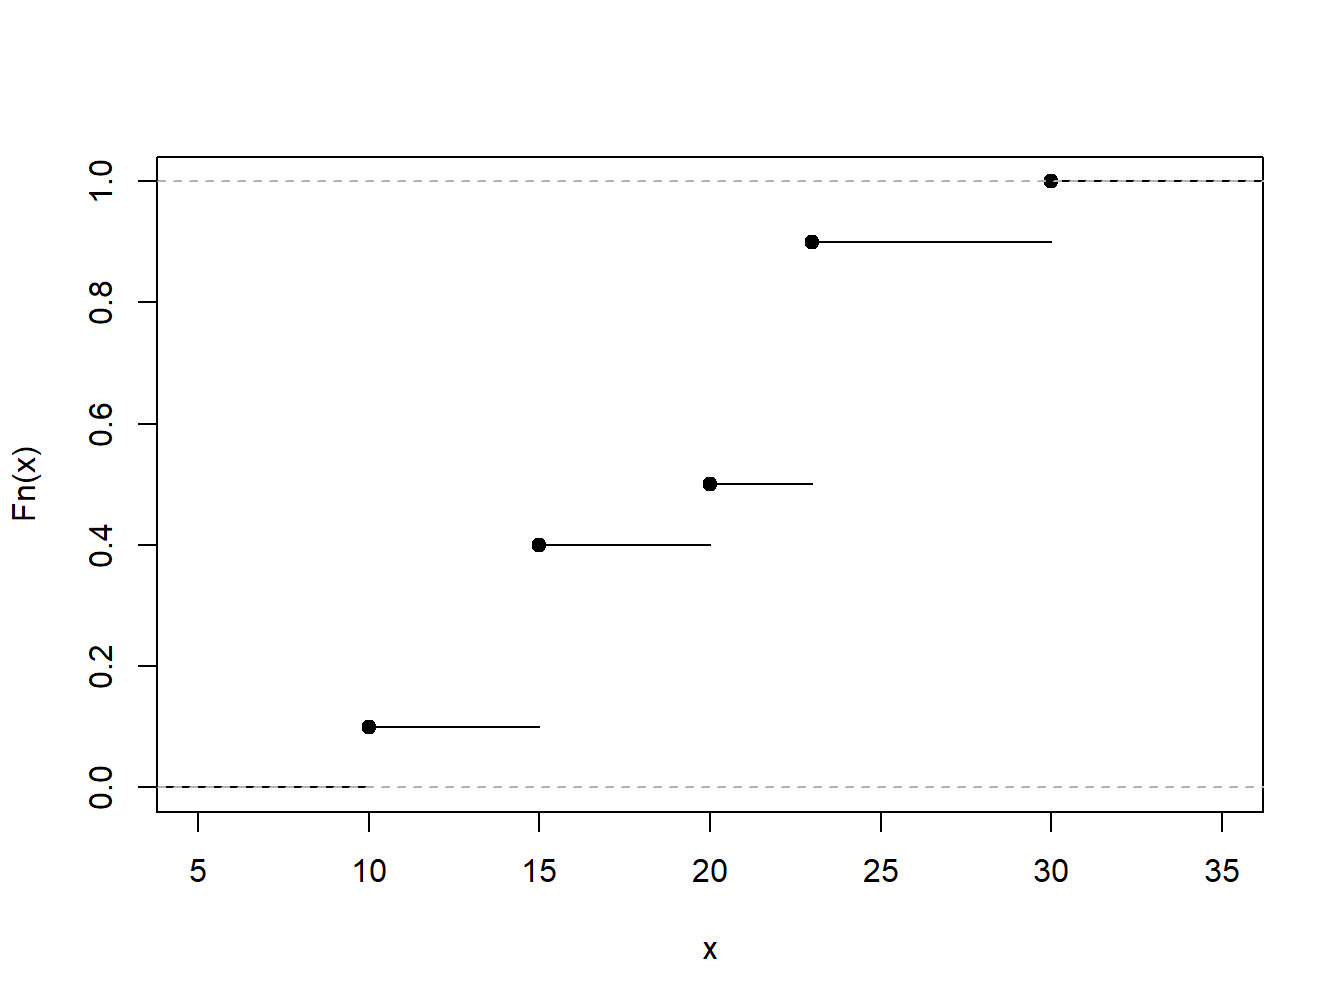
\includegraphics[width=0.6\linewidth]{LossDataAnalytics_files/figure-latex/EDFToy-1} 

}

\caption{Empirical Distribution Function of a Toy Example}\label{fig:EDFToy}
\end{figure}

Show R Code

\hypertarget{toggleToy}{}
\begin{verbatim}
(xExample <- c(10,rep(15,3),20,rep(23,4),30))
PercentilesxExample <- ecdf(xExample)
plot(PercentilesxExample, main="",xlab="x")
\end{verbatim}

\begin{center}\rule{0.5\linewidth}{\linethickness}\end{center}

\subsubsection{Quantiles}\label{S:QuantileEstimator}

We have already seen the \textbf{median}, which is the number such that
approximately half of a data set is below (or above) it. The
\textbf{first quartile} is the number such that approximately 25\% of
the data is below it and the \textbf{third quartile} is the number such
that approximately 75\% of the data is below it. A \(100p\)
\textbf{percentile} is the number such that \(100 \times p\) percent of
the data is below it.

To generalize this concept, consider a distribution function
\(F(\cdot)\), which may or may not be from a continuous variable, and
let \(q\) be a fraction so that \(0<q<1\). We want to define a quantile,
say \(q_F\), to be a number such that \(F(q_F) \approx q\). Notice that
when \(q = 0.5\), \(q_F\) is the median; when \(q = 0.25\), \(q_F\) is
the first quartile, and so on.

To be precise, for a given \(0<q<1\), define the \(q\)\textbf{th
quantile} \(q_F\) to be any number that satisfies

\begin{equation} 
  F(q_F-) \le q \le F(q_F)
  \label{eq:Quantile}
\end{equation}

Here, the notation \(F(x-)\) means to evaluate the function \(F(\cdot)\)
as a left-hand limit.

To get a better understanding of this definition, let us look at a few
special cases. First, consider the case where \(X\) is a continuous
random variable so that the distribution function \(F(\cdot)\) has no
jump points, as illustrated in Figure \ref{fig:Quantile1}. In this
figure, a few fractions, \(q_1\), \(q_2\), and \(q_3\) are shown with
their corresponding quantiles \(q_{F,1}\), \(q_{F,2}\), and \(q_{F,3}\).
In each case, it can be seen that \(F(q_F-)= F(q_F)\) so that there is a
unique quantile. Because we can find a unique inverse of the
distribution function at any \(0<q<1\), we can write \(q_F= F^{-1}(q)\).

\begin{figure}

{\centering 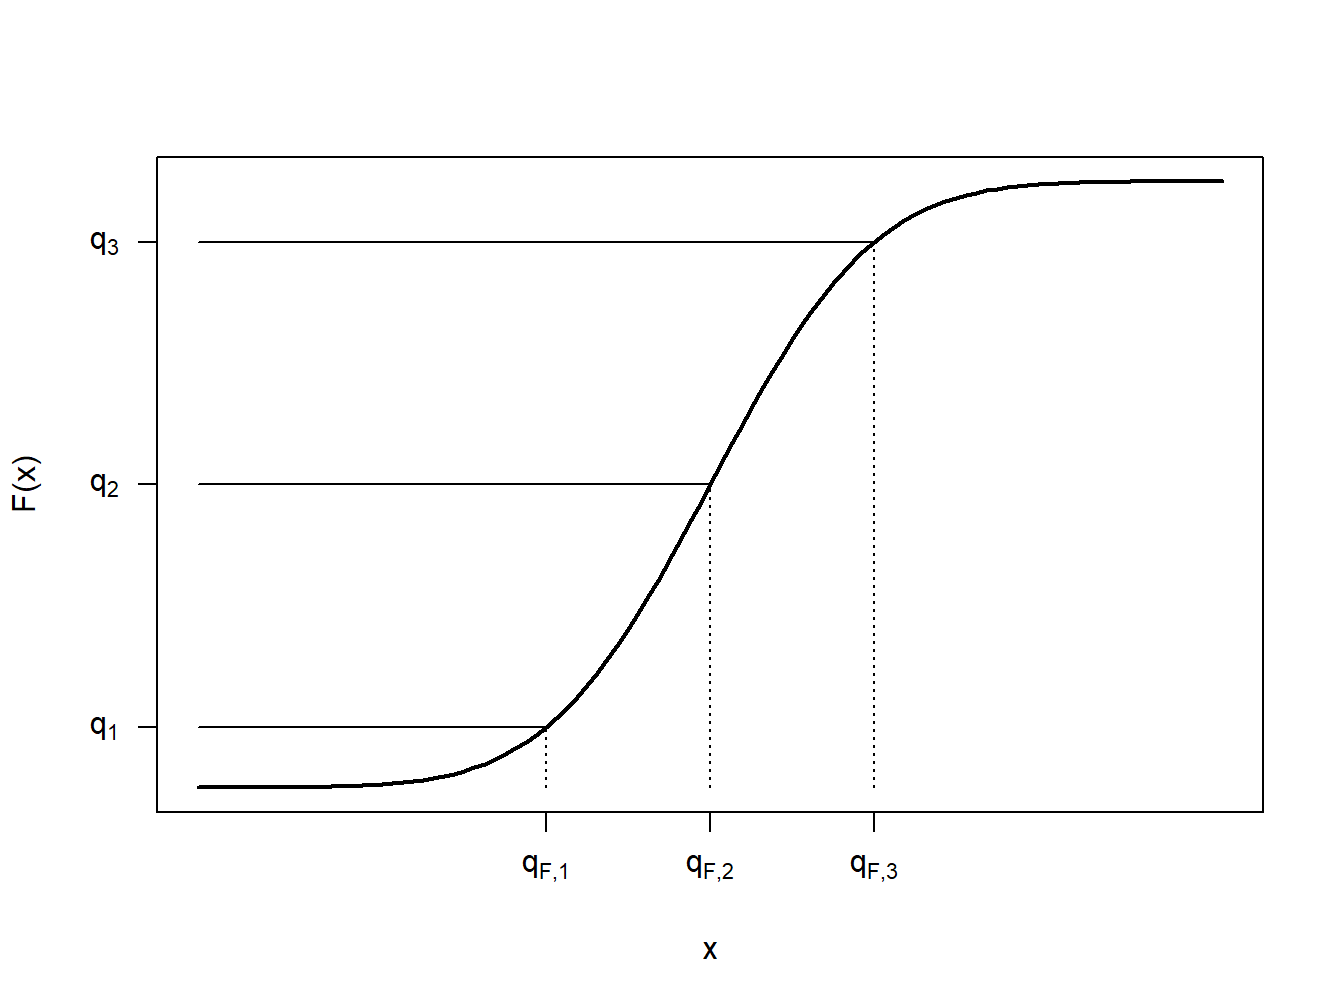
\includegraphics[width=0.6\linewidth]{LossDataAnalytics_files/figure-latex/Quantile1-1} 

}

\caption{Continuous Quantile Case}\label{fig:Quantile1}
\end{figure}

Figure \ref{fig:Quantile2} shows three cases for distribution functions.
The left panel corresponds to the continuous case just discussed. The
middle panel displays a jump point similar to those we already saw in
the empirical distribution function of Figure \ref{fig:EDFToy}. For the
value of \(q\) shown in this panel, we still have a unique value of the
quantile \(q_F\). Even though there are many values of \(q\) such that
\(F(q_F-) \le q \le F(q_F)\), for a particular value of \(q\), there is
only one solution to equation \eqref{eq:Quantile}. The right panel depicts
a situation in which the quantile can not be uniquely determined for the
\(q\) shown as there is a range of \(q_F\)'s satisfying equation
\eqref{eq:Quantile}.

\begin{figure}

{\centering 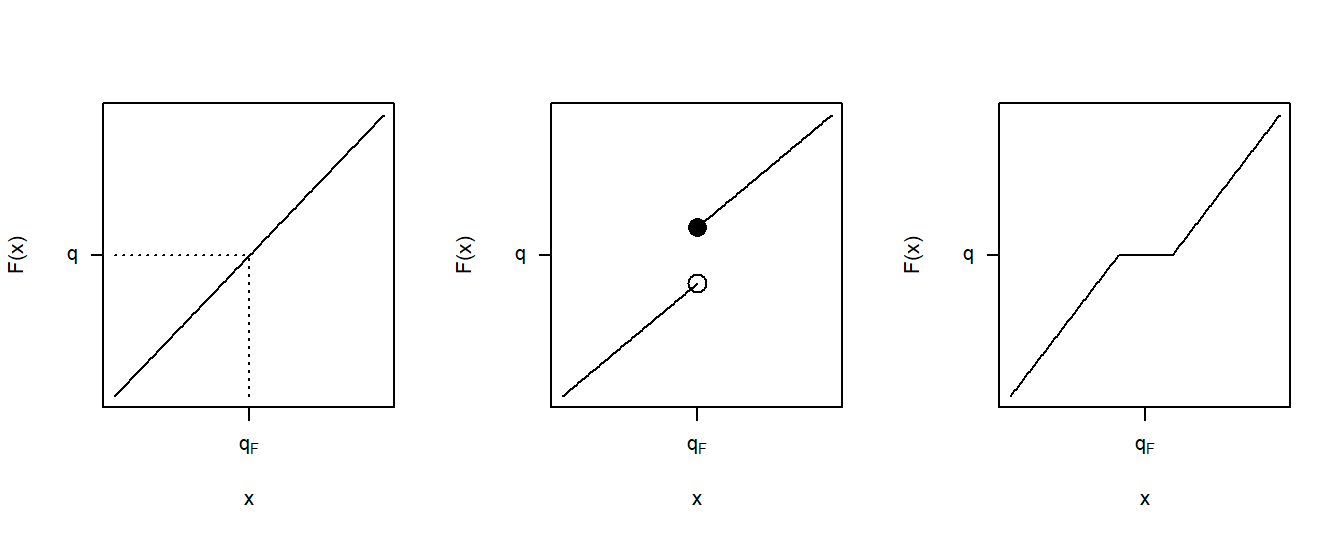
\includegraphics[width=0.9\linewidth]{LossDataAnalytics_files/figure-latex/Quantile2-1} 

}

\caption{Figure 3: Three Quantile Cases}\label{fig:Quantile2}
\end{figure}

\begin{center}\rule{0.5\linewidth}{\linethickness}\end{center}

\textbf{Example -- Toy Data Set: Continued.} Determine quantiles
corresponding to the 20th, 50th, and 95th percentiles.

Show Example Solution

\hypertarget{toggleExampleToyq}{}
\emph{Solution}. Consider Figure \ref{fig:EDFToy}. The case of
\(q=0.20\) corresponds to the middle panel, so the 20th percentile is
15. The case of \(q=0.50\) corresponds to the right panel, so the median
is any number between 20 and 23 inclusive. Many software packages use
the average 21.5 (e.g. \texttt{R}, as seen below). For the 95th
percentile, the solution is 30. We can see from the graph that 30 also
corresponds to the 99th and the 99.99th percentiles.

\begin{Shaded}
\begin{Highlighting}[]
\KeywordTok{quantile}\NormalTok{(xExample, }\DataTypeTok{probs=}\KeywordTok{c}\NormalTok{(}\FloatTok{0.2}\NormalTok{, }\FloatTok{0.5}\NormalTok{, }\FloatTok{0.95}\NormalTok{), }\DataTypeTok{type=}\DecValTok{2}\NormalTok{)}
\end{Highlighting}
\end{Shaded}

\begin{verbatim}
##  20%  50%  95% 
## 15.0 21.5 30.0
\end{verbatim}

\begin{center}\rule{0.5\linewidth}{\linethickness}\end{center}

By taking a weighted average between data observations, smoothed
empirical quantiles can handle cases such as the right panel in Figure
\ref{fig:Quantile2}. The \(q\)th \textbf{smoothed empirical quantile} is
defined as \[\hat{\pi}_q = (1-h) X_{(j)} + h X_{(j+1)}\] where
\(j=\lfloor(n+1)q\rfloor\), \(h=(n+1)q-j\), and
\(X_{(1)}, \ldots, X_{(n)}\) are the ordered values (the \textbf{order
statistics}) corresponding to \(X_1, \ldots, X_n\). Note that this is a
linear interpolation between \(X_{(j)}\) and \(X_{(j+1)}\).

\begin{center}\rule{0.5\linewidth}{\linethickness}\end{center}

\textbf{Example -- Toy Data Set: Continued.} Determine the 50th smoothed
percentile.

Show Example Solution

\hypertarget{toggleExampleToyp}{}
\emph{Solution:} Take \(n=10\) and \(q=0.5\). Then,
\(j=\lfloor(11)0.5 \rfloor= \lfloor5.5 \rfloor=5\) and
\(h=(11)(0.5)-5=0.5\). Then the 0.5-th smoothed empirical quantile is
\[\hat{\pi}_{0.5} = (1-0.5) X_{(5)} + (0.5) X_{(6)} = 0.5 (20) + (0.5)(23) = 21.5.\]
Now take \(n=10\) and \(q=0.2\). In this case,
\(j=\lfloor(11)0.2\rfloor=\lfloor 2.2 \rfloor=2\) and
\(h=(11)(0.2)-2=0.2\). Then the 0.2-th smoothed empirical quantile is
\[\hat{\pi}_{0.2} = (1-0.2) X_{(2)} + (0.2) X_{(3)} = 0.2 (15) + (0.8)(15) = 15.\]

\begin{center}\rule{0.5\linewidth}{\linethickness}\end{center}

\subsubsection{Density Estimators}\label{density-estimators}

When the random variable is discrete, estimating the probability mass
function \(f(x) = \Pr(X=x)\) is straightforward. We simply use the
empirical average, defined to be
\[f_n(x) = \frac{1}{n} \sum_{i=1}^n I(X_i = x).\]

For a continuous random variable, consider a discretized formulation in
which the domain of \(F(\cdot)\) is partitioned by constants
\(\{c_0 < c_1 < \cdots < c_k\}\) into intervals of the form
\([c_{j-1}, c_j)\), for \(j=1, \ldots, k\). The data observations are
thus ``grouped'' by the intervals into which they fall. Then, we might
use the basic definition of the empirical mass function, or a variation
such as
\[f_n(x) = \frac{n_j}{n \times (c_j - c_{j-1})}  \ \ \ \ \ \ c_{j-1} \le x < c_j,\]
where \(n_j\) is the number of observations (\(X_i\)) that fall into the
interval \([c_{j-1}, c_j)\).

Extending this notion to instances where we observe individual data,
note that we can always create arbitrary groupings and use this formula.
More formally, let \(b>0\) be a small positive constant, known as a
\textbf{bandwidth}, and define a density estimator to be

\begin{equation} 
  f_n(x) = \frac{1}{2nb} \sum_{i=1}^n I(x-b < X_i \le x + b)
  \label{eq:KDF}
\end{equation}

Show A Snippet of Theory

\hypertarget{Theorykerneldensity}{}
The idea is that the estimator \(f_n(x)\) in equation \eqref{eq:KDF} is
the average over \(n\) \emph{iid} realizations of a random variable with
mean

\[\begin{aligned}
\mathrm{E~ } \frac{1}{2b} I(x-b < X \le x + b) &=  \frac{1}{2b}\left(F(x+b)-F(x-b)\right) \\
&=  \frac{1}{2b} \left( \left\{ F(x) + b F^{\prime}(x) + b^2 C_1\right\}
\left\{ F(x) - b F^{\prime}(x) + b^2 C_2\right\} \right) \\
&=  F^{\prime}(x) + b \frac{C_1-C_2}{2} \rightarrow  F^{\prime}(x) = f(x),
\end{aligned}\]

as \(b\rightarrow 0\). That is, \(f_n(x)\) is an asymptotically unbiased
estimator of \(f(x)\) (its expectation approaches the true value as
sample size increases to infinity). This development assumes some
smoothness of \(F(\cdot)\), in particular, twice differentiability at
\(x\), but makes no assumptions on the form of the distribution function
\(F\). Because of this, the density estimator \(f_n\) is said to be
\emph{nonparametric}.

More generally, define the \textbf{kernel density estimator} as

\begin{equation} 
  f_n(x) = \frac{1}{nb} \sum_{i=1}^n w\left(\frac{x-X_i}{b}\right)
  \label{eq:kernelDens}
\end{equation}

where \(w\) is a probability density function centered about 0. Note
that equation \eqref{eq:KDF} simply becomes the kernel density estimator
where \(w(x) = \frac{1}{2}I(-1 < x \le 1)\), also known as the
\textbf{uniform kernel}. Other popular choices are shown in the table
below.

\[\text{Table 1: Popular Choices for the Kernel Density Estimator} \\
\begin{array}{l|cc}
\hline
\text{Kernel} &  w(x) \\
\hline 
\text{Uniform } &  \frac{1}{2}I(-1 < x \le 1) \\
\text{Triangle} &  (1-|x|)\times I(|x| \le 1) \\
\text{Epanechnikov} & \frac{3}{4}(1-x^2) \times I(|x| \le 1) \\
\text{Gaussian} & \phi(x) \\
\hline
\end{array}\]

Here, \(\phi(\cdot)\) is the standard normal density function. As we
will see in the following example, the choice of bandwidth \(b\) comes
with a \emph{bias-variance tradeoff} between matching local
distributional features and reducing the volatility.

\begin{center}\rule{0.5\linewidth}{\linethickness}\end{center}

\textbf{Example -- Property Fund.} Figure \ref{fig:Density2} shows a
histogram (with shaded gray rectangles) of logarithmic property claims
from 2010. The (blue) thick curve represents a Gaussian kernel density
where the bandwidth was selected automatically using an ad hoc rule
based on the sample size and volatility of the data. For this dataset,
the bandwidth turned out to be \(b=0.3255\). For comparison, the (red)
dashed curve represents the density estimator with a bandwidth equal to
0.1 and the green smooth curve uses a bandwidth of 1. As anticipated,
the smaller bandwidth (0.1) indicates taking local averages over less
data so that we get a better idea of the local average, but at the price
of higher volatility. In contrast, the larger bandwidth (1) smooths out
local fluctuations, yielding a smoother curve that may miss
perturbations in the local average. For actuarial applications, we
mainly use the kernel density estimator to get a quick visual impression
of the data. From this perspective, you can simply use the default ad
hoc rule for bandwidth selection, knowing that you have the ability to
change it depending on the situation at hand.

\begin{figure}

{\centering 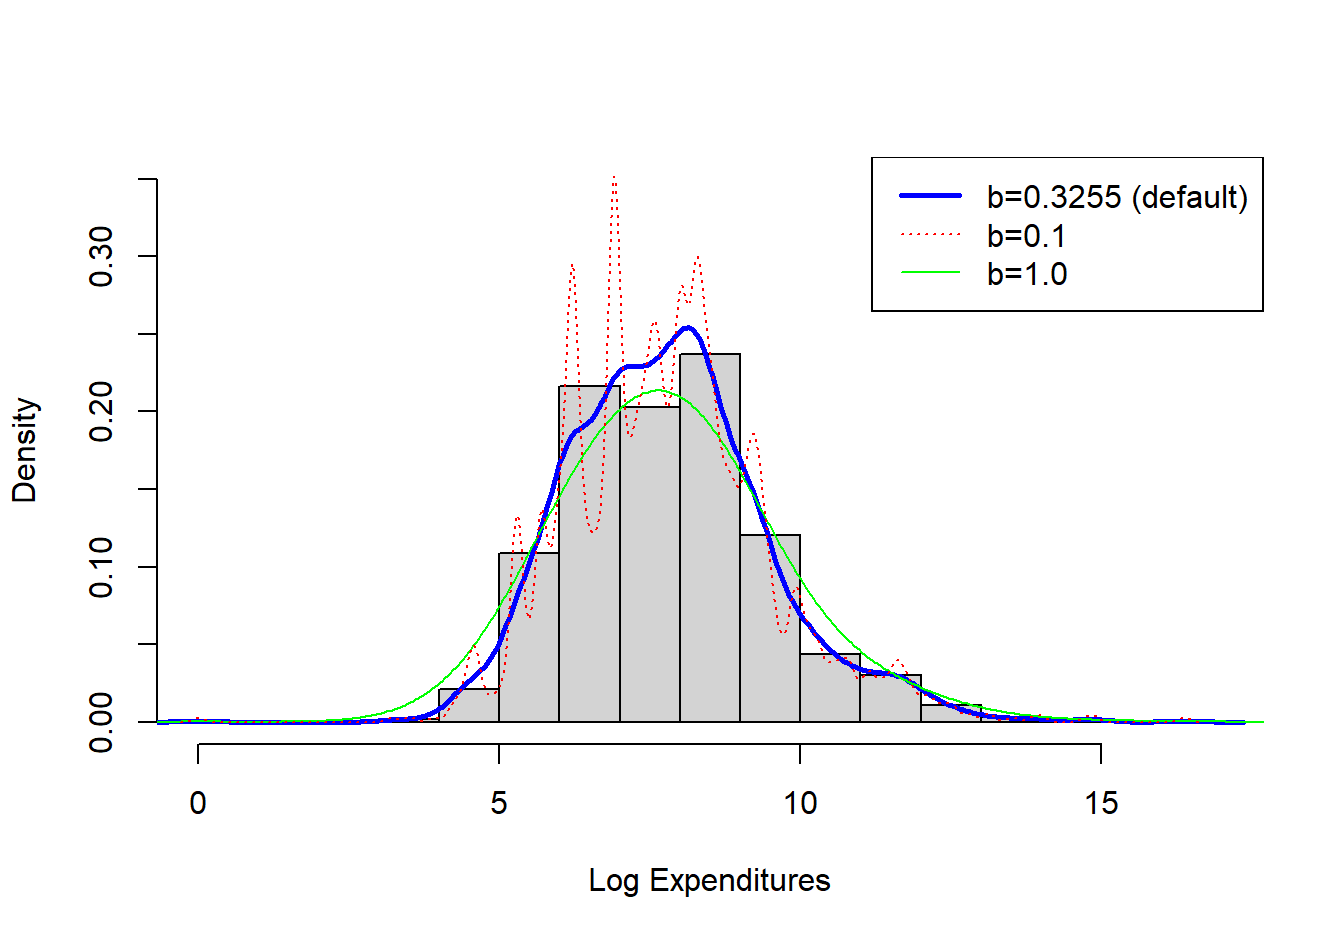
\includegraphics[width=0.7\linewidth]{LossDataAnalytics_files/figure-latex/Density2-1} 

}

\caption{Figure 4: Histogram of Logarithmic Property Claims with Superimposed Kernel Density Estimators}\label{fig:Density2}
\end{figure}

Show R Code

\hypertarget{togglekpdf}{}
\begin{verbatim}
#Density Comparison
hist(log(ClaimData$Claim), main="", ylim=c(0,.35),xlab="Log Expenditures", freq=FALSE, col="lightgray")
lines(density(log(ClaimData$Claim)), col="blue",lwd=2.5)
lines(density(log(ClaimData$Claim), bw=1), col="green")
lines(density(log(ClaimData$Claim), bw=.1), col="red", lty=3)
legend("topright", c("b=0.3255 (default)", "b=0.1", "b=1.0"), lty=c(1,3,1),
            lwd=c(2.5,1,1), col=c("blue", "red", "green"), cex=1)
\end{verbatim}

\begin{center}\rule{0.5\linewidth}{\linethickness}\end{center}

Nonparametric density estimators, such as the kernel estimator, are
regularly used in practice. The concept can also be extended to give
smooth versions of an empirical distribution function. Given the
definition of the kernel density estimator, the kernel estimator of the
distribution function can be found as \[\begin{aligned}
\hat{F}_n(x) = \frac{1}{n} \sum_{i=1}^n W\left(\frac{x-X_i}{b}\right).\end{aligned}\]

where \(W\) is the distribution function associated with the kernel
density \(w\). To illustrate, for the uniform kernel, we have
\(w(y) = \frac{1}{2}I(-1 < y \le 1)\), so \[\begin{aligned}
W(y) =
\begin{cases}
0 &            y<-1\\
\frac{y+1}{2}& -1 \le y < 1 \\
1 & y \ge 1 \\
\end{cases}\end{aligned}\]

\begin{center}\rule{0.5\linewidth}{\linethickness}\end{center}

\textbf{Exercise -- Exam C Question 3.} You study five lives to estimate
the time from the onset of a disease to death. The times to death are:

\[\begin{array}{ccccc}
2 & 3 & 3 & 3 & 7  \\
\end{array}\]

Using a triangular kernel with bandwith \(2\), calculate the density
function estimate at 2.5.

Show Solution

\hypertarget{toggleExamC3}{}
\emph{Solution:} For the kernel density estimate, we have
\[f_n(x) = \frac{1}{nb} \sum_{i=1}^n w\left(\frac{x-X_i}{b}\right),\]
where \(n=5\), \(b=2\), and \(x=2.5\). For the triangular kernel,
\(w(x) = (1-|x|)\times I(|x| \le 1)\). Thus,

\[\begin{array}{c|c|c}
\hline
X_i & \frac{x-X_i}{b} & w\left(\frac{x-X_i}{b} \right) \\
\hline 
2 & \frac{2.5-2}{2}=\frac{1}{4} &  (1-\frac{1}{4})(1) = \frac{3}{4} \\
\hline
3 & & \\
3 & \frac{2.5-3}{2}=\frac{-1}{4} & \left(1-\left| \frac{-1}{4} \right| \right)(1) = \frac{3}{4} \\
3 & & \\
\hline
7 & \frac{2.5-7}{2}=-2.25 & (1-|-2.25|)(0) = 0\\
\hline
\end{array}\]

Then the kernel density estimate is
\[f_n(x) = \frac{1}{5(2)}\left( \frac{3}{4} + (3) \frac{3}{4} + 0 \right) = \frac{3}{10}\]

\begin{center}\rule{0.5\linewidth}{\linethickness}\end{center}

\subsection{Tools for Model Selection}\label{S:ToolsModelSelection}

The previous section introduced nonparametric estimators in which there
was no parametric form assumed about the underlying distributions.
However, in many actuarial applications, analysts seek to employ a
parametric fit of a distribution for ease of explanation and the ability
to readily extend it to more complex situations such as including
explanatory variables in a regression setting. When fitting a parametric
distribution, one analyst might try to use a gamma distribution to
represent a set of loss data. However, another analyst may prefer to use
a Pareto distribution. How does one know which model to select?

Nonparametric tools can be used to corroborate the selection of
parametric models. Essentially, the approach is to compute selected
summary measures under a fitted parametric model and to compare it to
the corresponding quantity under the nonparametric model. As the
nonparametric does not assume a specific distribution and is merely a
function of the data, it is used as a benchmark to assess how well the
parametric distribution/model represents the data. This comparison may
alert the analyst to deficiencies in the parametric model and sometimes
point ways to improving the parametric specification.

\subsubsection{Graphical Comparison of
Distributions}\label{graphical-comparison-of-distributions}

We have already seen the technique of overlaying graphs for comparison
purposes. To reinforce the application of this technique, Figure
\ref{fig:ComparisonCDFPDF} compares the empirical distribution to two
parametric fitted distributions. The left panel shows the distribution
functions of claims distributions. The dots forming an ``S-shaped''
curve represent the empirical distribution function at each observation.
The thick blue curve gives corresponding values for the fitted gamma
distribution and the light purple is for the fitted Pareto distribution.
Because the Pareto is much closer to the empirical distribution function
than the gamma, this provides evidence that the Pareto is the better
model for this data set. The right panel gives similar information for
the density function and provides a consistent message. Based on these
figures, the Pareto distribution is the clear choice for the analyst.

\begin{figure}

{\centering 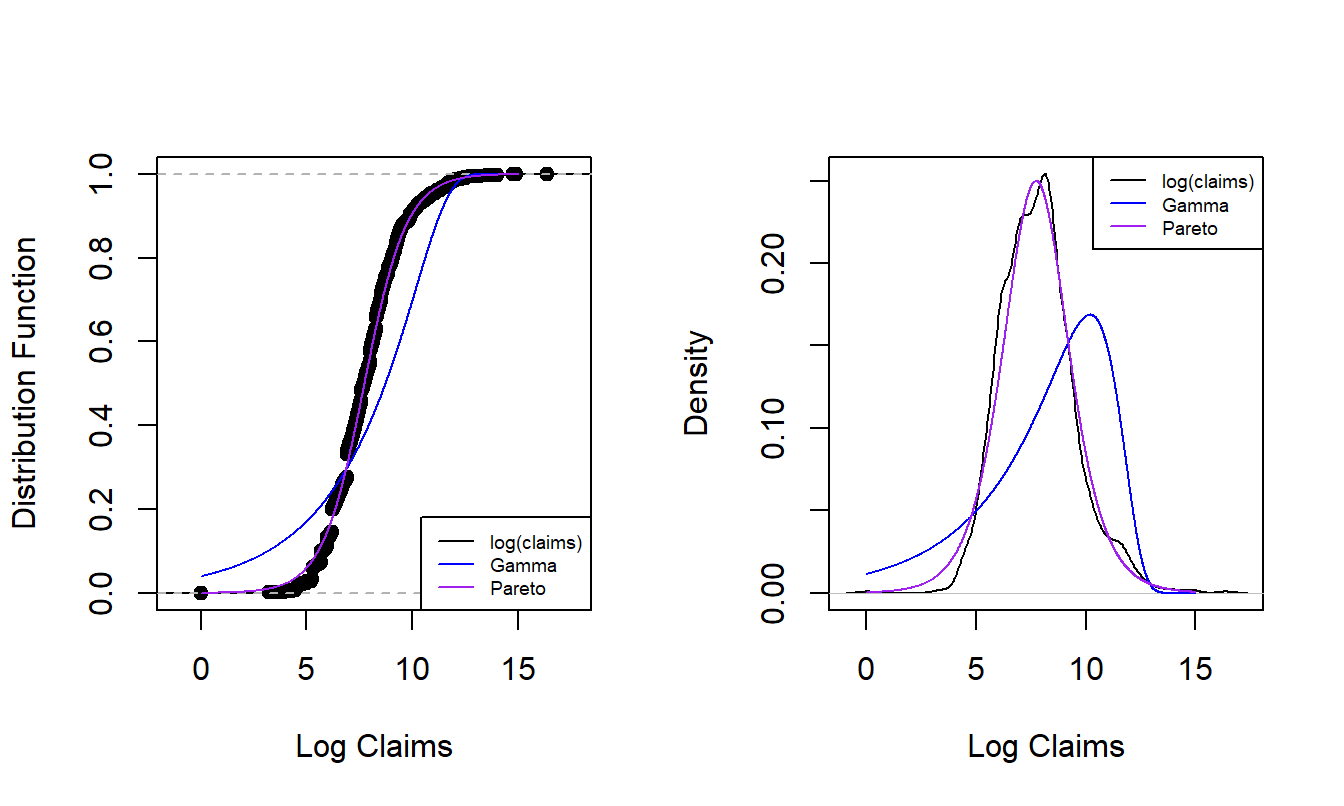
\includegraphics[width=0.8\linewidth]{LossDataAnalytics_files/figure-latex/ComparisonCDFPDF-1} 

}

\caption{Figure 5: Nonparametric Versus Fitted Parametric Distribution and Density Functions. The left-hand panel compares distribution functions, with the dots corresponding to the empirical distribution, the thick blue curve corresponding to the fitted gamma and the light purple curve corresponding to the fitted Pareto. The right hand panel compares these three distributions summarized using probability density functions.}\label{fig:ComparisonCDFPDF}
\end{figure}

For another way to compare the appropriateness of two fitted models,
consider the \textbf{probability-probability (\(pp\)) plot}. A \(pp\)
plot compares cumulative probabilities under two models. For our
purposes, these two models are the nonparametric empirical distribution
function and the parametric fitted model. Figure \ref{fig:PPPlot} shows
\(pp\) plots for the Property Fund data. The fitted gamma is on the left
and the fitted Pareto is on the right, compared to the same empirical
distribution function of the data. The straight line represents equality
between the two distributions being compared, so points close to the
line are desirable. As seen in earlier demonstrations, the Pareto is
much closer to the empirical distribution than the gamma, providing
additional evidence that the Pareto is the better model.

\begin{figure}

{\centering 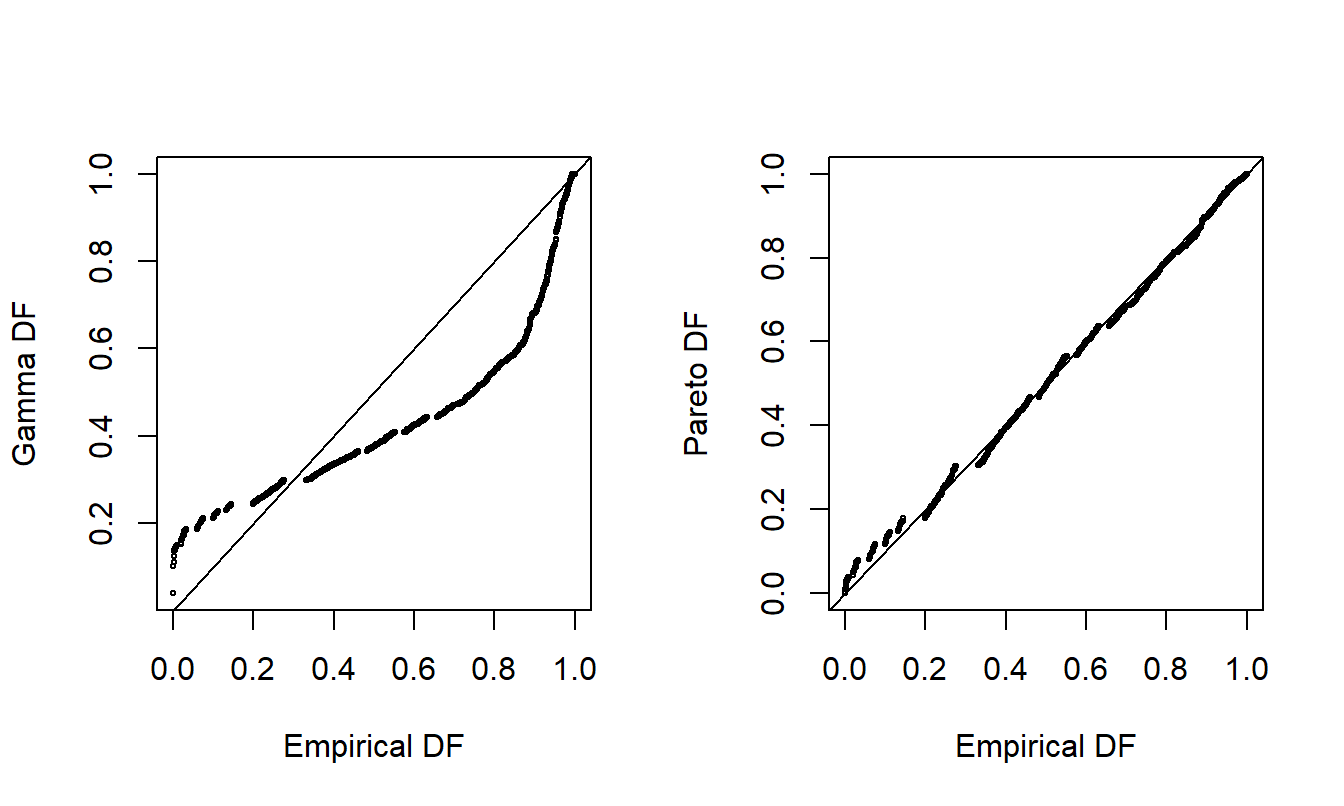
\includegraphics[width=0.8\linewidth]{LossDataAnalytics_files/figure-latex/PPPlot-1} 

}

\caption{Figure 6: Probability-Probability ($pp$) Plots. The horizontal axes gives the empirical distribution function at each observation. In the left-hand panel, the corresponding distribution function for the gamma is shown in the vertical axis. The right-hand panel shows the fitted Pareto distribution. Lines of $y=x$ are superimposed.}\label{fig:PPPlot}
\end{figure}

A \(pp\) plot is useful in part because no artificial scaling is
required, such as with the overlaying of densities in Figure
\ref{fig:ComparisonCDFPDF}, in which we switched to the log scale to
better visualize the data. Furthermore, \(pp\) plots are available in
multivariate settings where more than one outcome variable is available.
However, a limitation of the \(pp\) plot is that, because they plot
\emph{cumulative} distribution functions, it can sometimes be difficult
to detect \emph{where} a fitted parametric distribution is deficient. As
an alternative, it is common to use a \textbf{quantile-quantile (\(qq\))
plot}, as demonstrated in Figure \ref{fig:QQPlot}.

The \(qq\) plot compares two fitted models through their quantiles. As
with \(pp\) plots, we compare the nonparametric to a parametric fitted
model. Quantiles may be evaluated at each point of the data set, or on a
grid (e.g., at \(0, 0.001, 0.002, \ldots, 0.999, 1.000\)), depending on
the application. In Figure \ref{fig:QQPlot}, for each point on the
aforementioned grid, the horizontal axis displays the empirical quantile
and the vertical axis displays the corresponding fitted parametric
quantile (gamma for the upper two panels, Pareto for the lower two).
Quantiles are plotted on the original scale in the left panels and on
the log scale in the right panels to allow us to see where a fitted
distribution is deficient. The straight line represents equality between
the empirical distribution and fitted distribution. From these plots, we
again see that the Pareto is an overall better fit than the gamma.
Furthermore, the lower-right panel suggests that the Pareto distribution
does a good job with large observations, but provides a poorer fit for
small observations.

\begin{figure}

{\centering 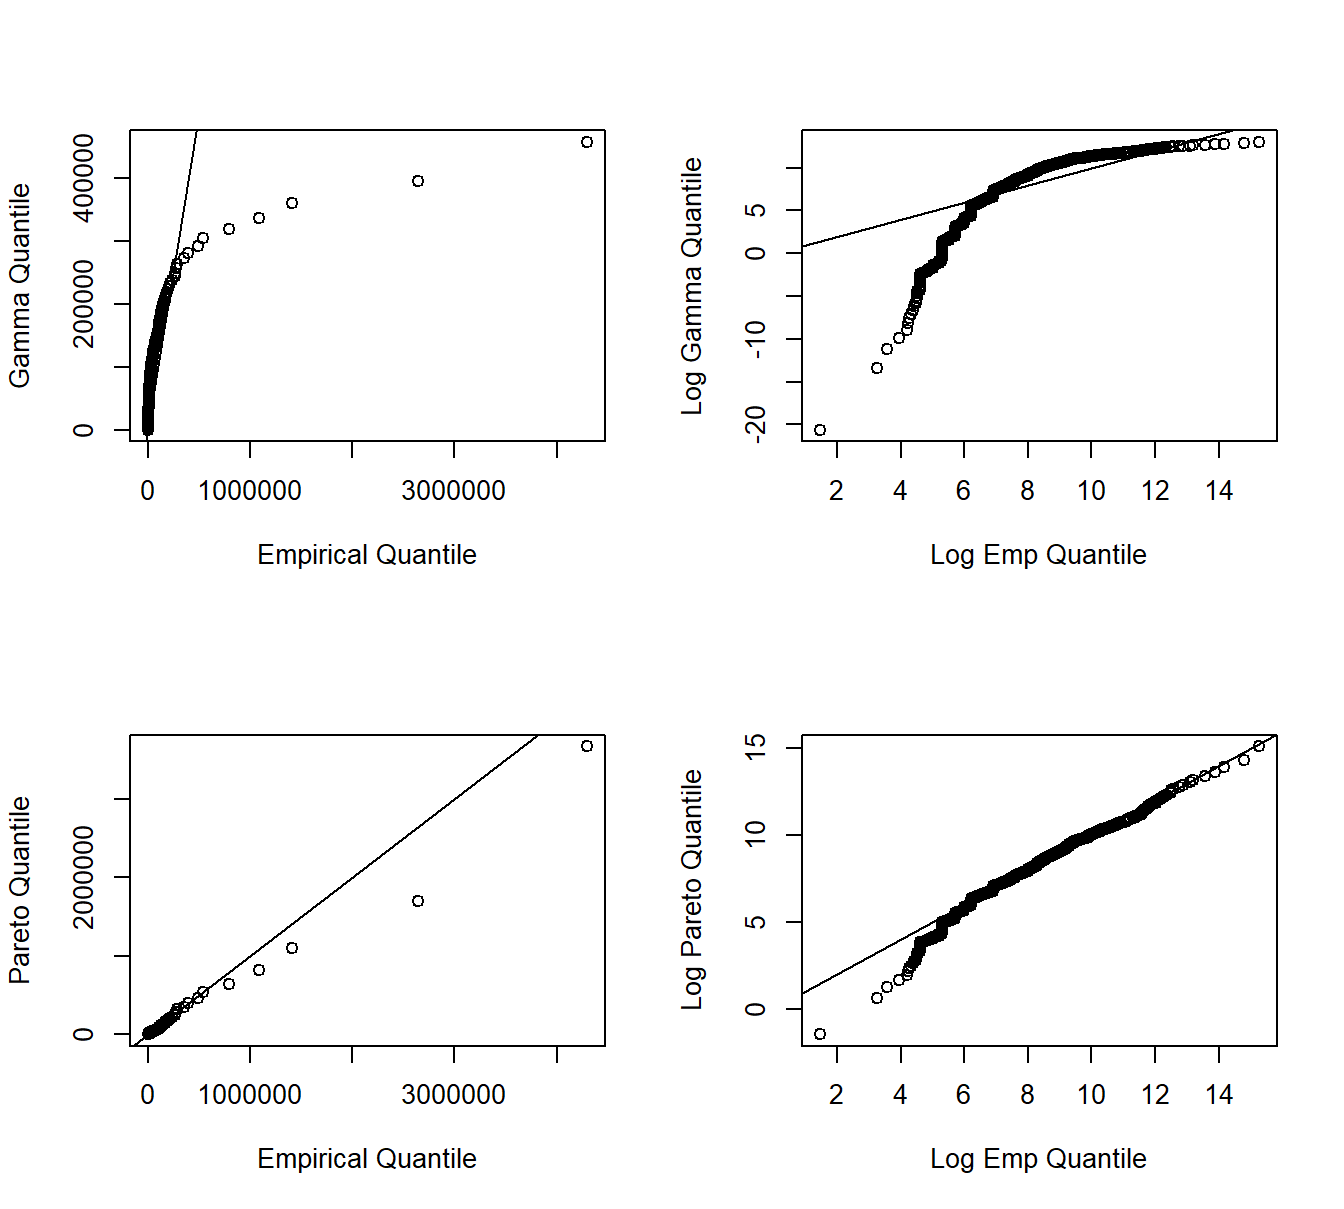
\includegraphics[width=0.8\linewidth]{LossDataAnalytics_files/figure-latex/QQPlot-1} 

}

\caption{Figure 7: Quantile-Quantile ($qq$) Plots. The horizontal axes gives the empirical quantiles at each observation. The right-hand panels they are graphed on a logarithmic basis. The vertical axis gives the quantiles from the fitted distributions; Gamma quantiles are in the upper panels, Pareto quantiles are in the lower panels.}\label{fig:QQPlot}
\end{figure}

\begin{center}\rule{0.5\linewidth}{\linethickness}\end{center}

\textbf{Exercise -- Exam C Question 59.} The graph below shows a \(pp\)
plot of a fitted distribution compared to a sample.

\begin{figure}

{\centering 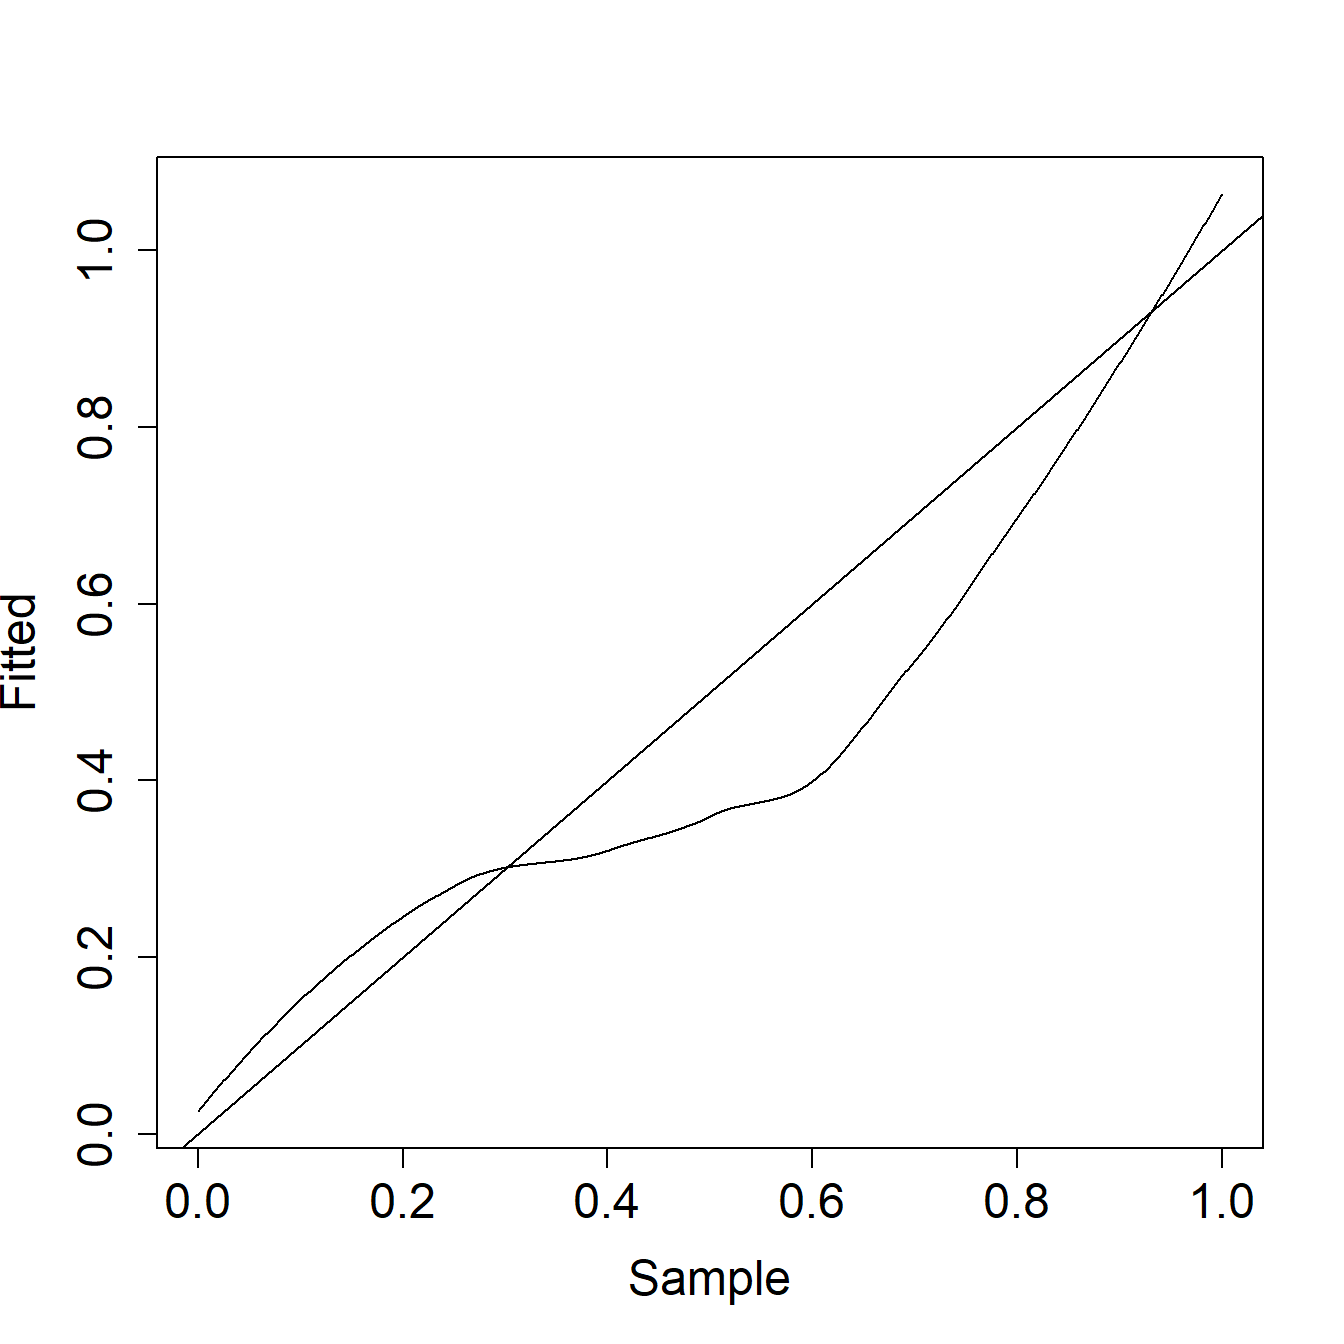
\includegraphics[width=0.4\linewidth]{LossDataAnalytics_files/figure-latex/unnamed-chunk-4-1} 

}

\end{figure}

Comment on the two distributions with respect to left tail, right tail,
and median probabilities.

Show Solution

\hypertarget{toggleExamC59}{}
\emph{Solution:} The tail of the fitted distribution is too thick on the
left, too thin on the right, and the fitted distribution has less
probability around the median than the sample. To see this, recall that
the \(pp\) plot graphs the cumulative distribution of two distributions
on its axes (empirical on the x-axis and fitted on the y-axis in this
case). For small values of \(x\), the fitted model assigns greater
probability to being below that value than occurred in the sample (i.e.
\(F(x) > F_n(x)\)). This indicates that the model has a heavier left
tail than the data. For large values of \(x\), the model again assigns
greater probability to being below that value and thus less probability
to being above that value (i.e. \(S(x) < S_n(x)\). This indicates that
the model has a lighter right tail than the data. In addition, as we go
from 0.4 to 0.6 on the horizontal axis (thus looking at the middle 20\%
of the data), the \(pp\) plot increases from about 0.3 to 0.4. This
indicates that the model puts only about 10\% of the probability in this
range.

\begin{center}\rule{0.5\linewidth}{\linethickness}\end{center}

\subsubsection{Statistical Comparison of
Distributions}\label{statistical-comparison-of-distributions}

When selecting a model, it is helpful to make the graphical displays
presented. However, for reporting results, it can be effective to
supplement the graphical displays with selected statistics that
summarize model goodness of fit. Table 2
\texttt{\textbackslash{}@ref(tab:GoFstats)} provides three commonly used
goodness of fit statistics. Here, \(F_n\) is the empirical distribution
and \(F\) is the fitted distribution.

\[\text{Table 2: Three Goodness of Fit Statistics} \\
\begin{array}{l|cc}
\hline
\text{Statistic} & \text{Definition} & \text{Computational Expression} \\
\hline 
\text{Kolmogorov-Smirnov} & \max_x |F_n(x) - F(x)| & \max(D^+, D^-) \text{ where } \\
&& D^+ = \max_{i=1, \ldots, n} \left|\frac{i}{n} - F_i\right| \\
&& D^- = \max_{i=1, \ldots, n} \left| F_i - \frac{i-1}{n} \right| \\
\text{Cramer-von Mises} & n \int (F_n(x) - F(x))^2 f(x) dx & \frac{1}{12n} + \sum_{i=1}^n \left(F_i - (2i-1)/n\right)^2 \\
\text{Anderson-Darling} & n \int \frac{(F_n(x) - F(x))^2}{F(x)(1-F(x))} f(x) dx & -n-\frac{1}{n} \sum_{i=1}^n (2i-1) \log\left(F_i(1-F_{n+1-i})\right)^2 \\
\hline
\end{array} \\
\text{where } F_i \text{ is defined to be } F(x_i).\]

The \textbf{Kolmogorov-Smirnov statistic} is the maximum absolute
difference between the fitted distribution function and the empirical
distribution function. Instead of comparing differences between single
points, the \textbf{Cramer-von Mises statistic} integrates the
difference between the empirical and fitted distribution functions over
the entire range of values. The \textbf{Anderson-Darling statistic} also
integrates this difference over the range of values, although weighted
by the inverse of the variance. It therefore places greater emphasis on
the tails of the distribution (i.e when \(F(x)\) or \(1-F(x)=S(x)\) is
small).

\begin{center}\rule{0.5\linewidth}{\linethickness}\end{center}

\textbf{Exercise -- Exam C Question 40 (modified).} A sample of claim
payments is:

\[\begin{array}{ccccc}
29 & 64 & 90 & 135 & 182  \\
\end{array}\]

Compare the empirical claims distribution to an exponential distribution
with mean \(100\) by calculating the value of the Kolmogorov-Smirnov
test statistic.

Show Solution

\hypertarget{toggleExamC40}{}
\emph{Solution:} For an exponential distribution with mean \(100\), the
cumulative distribution function is \(F(x)=1-e^{-x/100}\). Thus,

\[\begin{array}{ccccc}
\hline
x & F(x) & F_n(x) & F_n(x-) & \max(|F(x)-F_n(x)|,|F(x)-F_n(x-)|) \\
\hline 
29  & 0.2517 & 0.2 & 0   & \max(0.0517, 0.2517) = 0.2517 \\
64  & 0.4727 & 0.4 & 0.2 & \max(0.0727, 0.2727) = 0.2727 \\
90  & 0.5934 & 0.6 & 0.4 & \max(0.0066, 0.1934) = 0.1934 \\
135 & 0.7408 & 0.8 & 0.6 & \max(0.0592, 0.1408) = 0.1408 \\
182 & 0.8380 & 1   & 0.8 & \max(0.1620, 0.0380) = 0.1620 \\
\hline
\end{array}\]

The Kolmogorov-Smirnov test statistic is therefore
\(KS = \max(0.2517, 0.2727, 0.1934, 0.1408, 0.1620) = 0.2727\).

\begin{center}\rule{0.5\linewidth}{\linethickness}\end{center}

\subsection{Starting Values}\label{starting-values}

The method of moments and percentile matching are nonparametric
estimation methods that provide alternatives to maximum likelihood.
Generally, maximum likelihood is the preferred technique because it
employs data more efficiently. However, methods of moments and
percentile matching are useful because they are easier to interpret and
therefore allow the actuary or analyst to explain procedures to others.
Additionally, the numerical estimation procedure (e.g.~if performed in
\texttt{R}) for the maximum likelihood is iterative and requires
starting values to begin the recursive process. Although many problems
are robust to the choice of the starting values, for some complex
situations, it can be important to have a starting value that is close
to the (unknown) optimal value. Method of moments and percentile
matching are techniques that can produce desirable estimates without a
serious computational investment and can thus be used as a starting
value for computing maximum likelihood.

\subsubsection{Method of Moments}\label{method-of-moments}

Under the \textbf{method of moments}, we approximate the moments of the
parametric distribution using the empirical (nonparametric) moments
described in Section \ref{S:MomentEstimator}. We can then algebraically
solve for the parameter estimates.

\begin{center}\rule{0.5\linewidth}{\linethickness}\end{center}

\textbf{Example -- Property Fund.} For the 2010 property fund, there are
\(n=1,377\) individual claims (in thousands of dollars) with

\[m_1 = \frac{1}{n} \sum_{i=1}^n X_i = 26.62259 \ \ \ \
\text{and} \ \ \ \
 m_2 = \frac{1}{n} \sum_{i=1}^n X_i^2 = 136154.6 .\] Fit the parameters
of the gamma distribution using the method of moments.

Show Example Solution

\hypertarget{toggleExampleMM}{}
To fit a gamma distribution, we have \(\mu_1 = \alpha \theta\) and
\(\mu_2^{\prime} = \alpha(\alpha+1) \theta^2\). Equating the two yields
the method of moments estimators, easy algebra shows that

\[\alpha = \frac{\mu_1^2}{\mu_2^{\prime}-\mu_1^2}  \ \ \ \text{and} \ \ \  \theta = \frac{\mu_2^{\prime}-\mu_1^2}{\mu_1}.\]

Thus, the method of moment estimators are

\[\begin{aligned}
\hat{\alpha} &=  \frac{26.62259^2}{136154.6-26.62259^2} = 0.005232809 \\
\hat{\theta} &=  \frac{136154.6-26.62259^2}{26.62259} = 5,087.629.
\end{aligned}\]

For comparison, the maximum likelihood values turn out to be
\(\hat{\alpha}_{MLE} = 0.2905959\) and
\(\hat{\theta}_{MLE} = 91.61378\), so there are big discrepancies
between the two estimation procedures. This is one indication, as we
have seen before, that the gamma model fits poorly.

In contrast, now assume a Pareto distribution so that
\(\mu_1 = \theta/(\alpha -1)\) and
\(\mu_2^{\prime} = 2\theta^2/((\alpha-1)(\alpha-2) )\). Easy algebra
shows

\[\alpha = 1+ \frac{\mu_2^{\prime}}{\mu_2^{\prime}-\mu_1^2} \ \ \ \
\text{and} \ \ \ \ \
 \theta = (\alpha-1)\mu_1.\]

Thus, the method of moment estimators are

\[\begin{aligned}
\hat{\alpha} &=  1+ \frac{136154.6}{136154.6-26,62259^2} = 2.005233 \\
\hat{\theta} &=  (2.005233-1) \cdot 26.62259 = 26.7619
\end{aligned}\]

The maximum likelihood values turn out to be
\(\hat{\alpha}_{MLE} = 0.9990936\) and
\(\hat{\theta}_{MLE} = 2.2821147\). It is interesting that
\(\hat{\alpha}_{MLE}<1\); for the Pareto distribution, recall that
\(\alpha <1\) means that the mean is infinite. This is another
indication that the property claims data set is a long tail
distribution.

\begin{center}\rule{0.5\linewidth}{\linethickness}\end{center}

As the above example suggests, there is flexibility with the method of
moments. For example, we could have matched the second and third moments
instead of the first and second, yielding different estimators.
Furthermore, there is no guarantee that a solution will exist for each
problem. You will also find that matching moments is possible for a few
problems where the data are censored or truncated, but in general, this
is a more difficult scenario. Finally, for distributions where the
moments do not exist or are infinite, method of moments is not
available. As an alternative for the infinite moment situation, one can
use the percentile matching technique.

\subsubsection{Percentile Matching}\label{percentile-matching}

Under percentile matching, we approximate the quantiles or percentiles
of the parametric distribution using the empirical (nonparametric)
quantiles or percentiles described in Section \ref{S:QuantileEstimator}.

\begin{center}\rule{0.5\linewidth}{\linethickness}\end{center}

Show Example

\hypertarget{toggleExamplePM}{}
\textbf{Example -- Property Fund.} For the 2010 property fund, we
illustrate matching on quantiles. In particular, the Pareto distribution
is intuitively pleasing because of the closed-form solution for the
quantiles. Recall that the distribution function for the Pareto
distribution is
\[F(x) = 1 - \left(\frac{\theta}{x+\theta}\right)^{\alpha}\] Easy
algebra shows that we can express the quantile as
\[F^{-1}(q) = \theta \left( (1-q)^{-1/\alpha} -1 \right)\] for a
fraction \(q\), \(0<q<1\).

The 25th percentile (the first quartile) turns out to be \(0.78853\) and
the 95th percentile is \(50.98293\) (both in thousands of dollars). With
two equations
\[0.78853 = \theta \left( 1- (1-.25)^{-1/\alpha} \right) \ \ \ \ \text{and} \ \ \ \ 50.98293 = \theta \left( 1- (1-.75)^{-1/\alpha} \right)\]
and two unknowns, the solution is
\[\hat{\alpha} = 0.9412076 \ \ \ \ \ \text{and} \ \ \ \
\hat{\theta} = 2.205617 .\] We remark here that a numerical routine is
required for these solutions as no analytic solution is available.
Furthermore, recall that the maximum likelihood estimates are
\(\hat{\alpha}_{MLE} = 0.9990936\) and
\(\hat{\theta}_{MLE} = 2.2821147\), so the percentile matching provides
a better approximation for the Pareto distribution than the method of
moments.

\begin{center}\rule{0.5\linewidth}{\linethickness}\end{center}

\textbf{Exercise -- Exam C Question 1.} You are given:

\begin{enumerate}
\def\labelenumi{(\roman{enumi})}
\tightlist
\item
  Losses follow a loglogistic distribution with cumulative distribution
  function:
  \[F(x) = \frac{\left(x/\theta\right)^{\gamma}}{1+\left(x/\theta\right)^{\gamma}}\]
\item
  The sample of losses is:
\end{enumerate}

\[\begin{array}{ccccccccccc}
10 &35 &80 &86 &90 &120 &158 &180 &200 &210 &1500 \\
\end{array}\]

Calculate the estimate of \(\theta\) by percentile matching, using the
40th and 80th empirically smoothed percentile estimates.

Show Solution

\hypertarget{toggleExamC1}{}
\emph{Solution:} With 11 observations, we have
\(j=\lfloor(n+1)q\rfloor = \lfloor 12(0.4) \rfloor = \lfloor 4.8\rfloor=4\)
and \(h=(n+1)q-j = 12(0.4)-4=0.8\). By interpolation, the 40th
empirically smoothed percentile estimate is
\(\hat{\pi}_{0.4} = (1-h) X_{(j)} + h X_{(j+1)} = 0.2(86)+0.8(90)=89.2\).

Similarly, for the 80th empirically smoothed percentile estimate, we
have \(12(0.8)=9.6\) so the estimate is
\(\hat{\pi}_{0.8} = 0.4(200)+0.6(210)=206\).

Using the loglogistic cumulative distribution, we need to solve the
following two equations for parameters \(\theta\) and \(gamma\):
\[0.4=\frac{(89.2/\theta)^\gamma}{1+(89.2/\theta)^\gamma} \ \ \ \text{and} \ \ \ \   0.8=\frac{(206/\theta)^\gamma}{1+(206+\theta)^\gamma}\]

Solving for each parenthetical expression gives
\(\frac{2}{3}=(89.2/\theta)^\gamma\) and \(4=(206/\theta)^\gamma\).
Taking the ratio of the second equation to the first gives
\(6=(206/89.2)^\gamma \Rightarrow \gamma=\frac{\ln(6)}{\ln(206/89.2)} = 2.1407\).
Then \(4^{1/2.1407}=206/\theta \Rightarrow \theta=107.8\)

\begin{center}\rule{0.5\linewidth}{\linethickness}\end{center}

\section{Model Validation}\label{S:ModelValidation}

In this section, you learn how to:

\begin{itemize}
\tightlist
\item
  Describe the iterative model selection specification process
\item
  Outline steps needed to select a parametric model
\item
  Describe pitfalls of model selection based purely on insample data
  when compared to the advantages of out-of-sample model validation
\item
  Describe the Gini statistic for model selection
\end{itemize}

This section revisits the idea that model selection is an iterative
process in which models are cyclically (re)formulated and tested for
appropriateness before using them for inference. After summarizing the
process of selecting a model based on the dataset at hand, we will focus
on the process of validating the selected model by applying it to a
different dataset.

\subsection{Iterative Model Selection}\label{iterative-model-selection}

In our development, we examine the data graphically, hypothesize a model
structure, and compare the data to a candidate model in order to
formulate an improved model. Box (1980) describes this as an
\emph{iterative process} which is shown in Figure \ref{fig:Iterative}.

\begin{figure}

{\centering 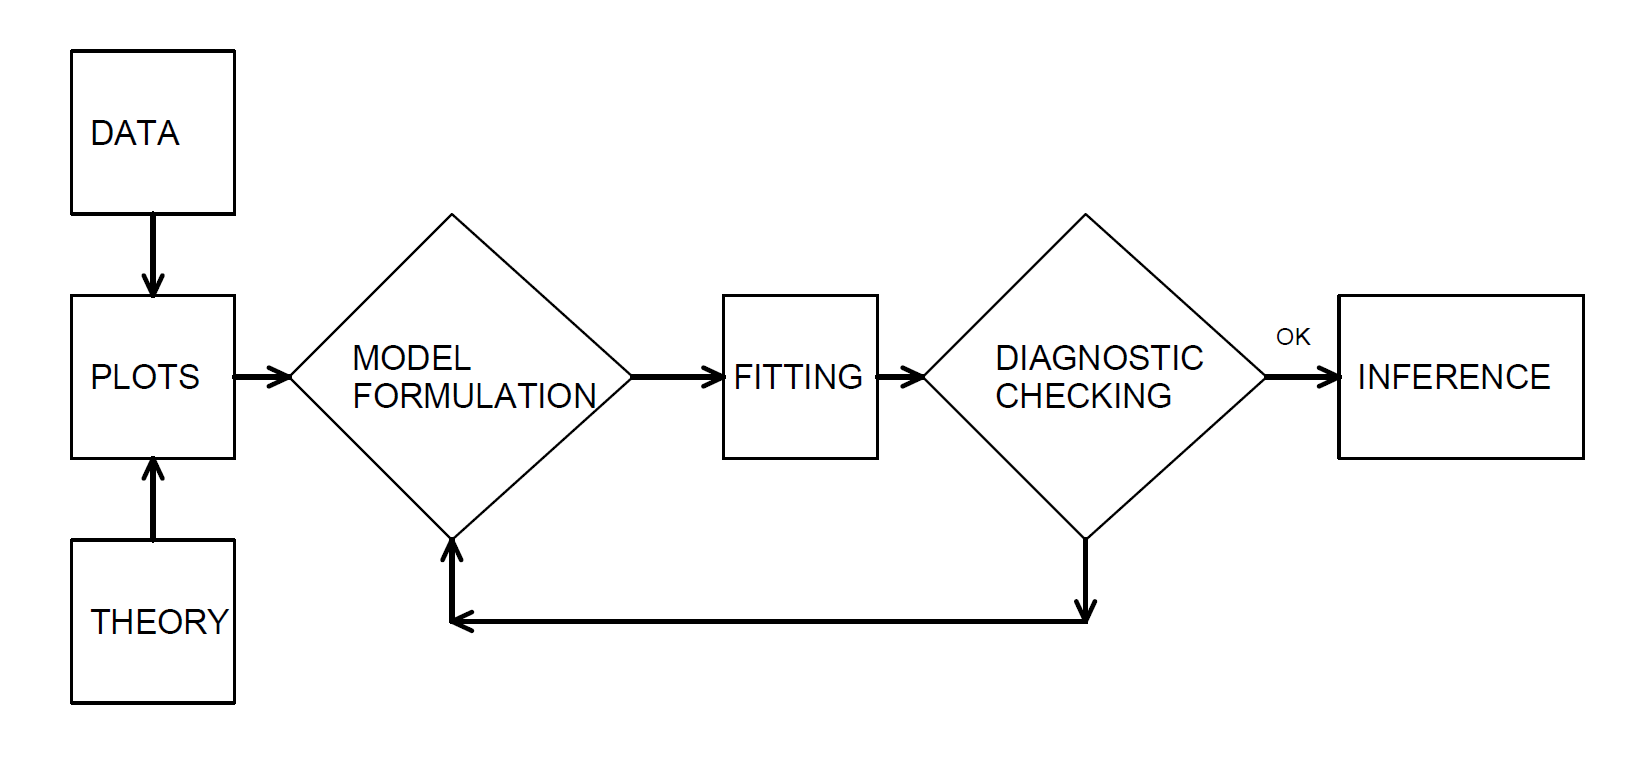
\includegraphics[width=0.8\linewidth]{Figures/F5Iterative} 

}

\caption{The iterative model specification process.}\label{fig:Iterative}
\end{figure}

This iterative process provides a useful recipe for structuring the task
of specifying a model to represent a set of data. The first step, the
model formulation stage, is accomplished by examining the data
graphically and using prior knowledge of relationships, such as from
economic theory or industry practice. The second step in the iteration
is based on the assumptions of the specified model. These assumptions
must be consistent with the data to make valid use of the model. The
third step, \textbf{diagnostic checking}, is also known as \emph{data
and model criticism}; the data and model must be consistent with one
another before additional inferences can be made. Diagnostic checking is
an important part of the model formulation; it can reveal mistakes made
in previous steps and provide ways to correct these mistakes.

The iterative process also emphasizes the skills you need to make
analytics work. First, you need a willingness to summarize information
numerically and portray this information graphically. Second, it is
important to develop an understanding of model properties. You should
understand how a probabilistic model behaves in order to match a set of
data to it. Third, theoretical properties of the model are also
important for inferring general relationships based on the behavior of
the data.

\subsection{Summarizing Model
Selection}\label{summarizing-model-selection}

Techniques available for selecting a model depend upon whether the
outcomes \(X\) are discrete, continuous, or a hybrid of the two,
although the principles are the same.

Begin by summarizing the data graphically and with statistics that do
not rely on a specific parametric form, as summarized in Section
\ref{S:NonParInf}. Specifically, you will want to graph both the
empirical distribution and density functions. Particularly for loss data
that contain many zeros and that can be skewed, deciding on the
appropriate scale (e.g., logarithmic) may present some difficulties. For
discrete data, tables are often preferred. Determine sample moments,
such as the mean and variance, as well as selected quantiles, including
the minimum, maximum, and the median. For discrete data, the mode (or
most frequently occurring value) is usually helpful.

These summaries, as well as your familiarity of industry practice, will
suggest one or more candidate parametric models. Generally, start with
the simpler parametric models (for example, one parameter exponential
before a two parameter gamma), gradually introducing more complexity
into the modeling process.

Critique the candidate parametric model numerically and graphically. For
the graphs, utilize the tools introduced in Section
\ref{S:ToolsModelSelection} such as \(pp\) and \(qq\) plots. For the
numerical assessments, examine the statistical significance of
parameters and try to eliminate parameters that do not provide
additional information.

For comparing model fits, if one model is a subset of another, then a
\textbf{likelihood ratio test} may be employed. Generally, models are
not proper subsets of one another so overall goodness of fit statistics,
summarized in Section 1.2
\texttt{\textbackslash{}ref\{S:NonparametricModelSelection\}}, are
useful for model comparison. For discrete data, a \textbf{chi-square
goodness of fit statistic} is generally preferred as it is more
intuitive and simpler to explain.

\emph{Information criteria}, such as Akaike's Information Criterion
(\textbf{AIC}) and the Schwarz Bayesian Criterion (\textbf{BIC}) are
widely cited because they can be readily generalized to multivariate
settings.

Finally, a likelihood statistic that we have not yet considered is
\textbf{Vuong's test}. This statistic is gaining popularity among
analysts because it is a likelihood based statistic that has the ability
to compare models that are non-nested.

\subsection{Out of Sample Validation}\label{out-of-sample-validation}

\textbf{Model validation} is the process of confirming that the proposed
model is appropriate, especially in light of the purposes of the
investigation. An important criticism of the model selection process is
that it can be susceptible to \emph{data-snooping}, that is, fitting a
great number of models to a single set of data. By looking at a large
number of models, we may overfit the data and understate the natural
variation in our representation.

We can respond to this criticism by using a technique called
\textbf{out-of-sample validation}. The ideal situation is to have
available two sets of data, one for model development and one for model
validation. We initially develop one or several models on a first data
set. The models developed from the first set of data are called our
\emph{candidate} models. Then, the relative performance of the candidate
models could be measured on a second set of data. In this way, the data
used to validate the model is unaffected by the procedures used to
formulate the model.

Unfortunately, rarely will two sets of data be available to the
investigator. However, we can implement the validation process by
splitting the data set into two subsamples. We call these the
\textbf{model development subsample} and \textbf{validation subsample},
respectively. Figure \ref{fig:ModelValidation} illustrates this
splitting of the data.

\begin{figure}

{\centering 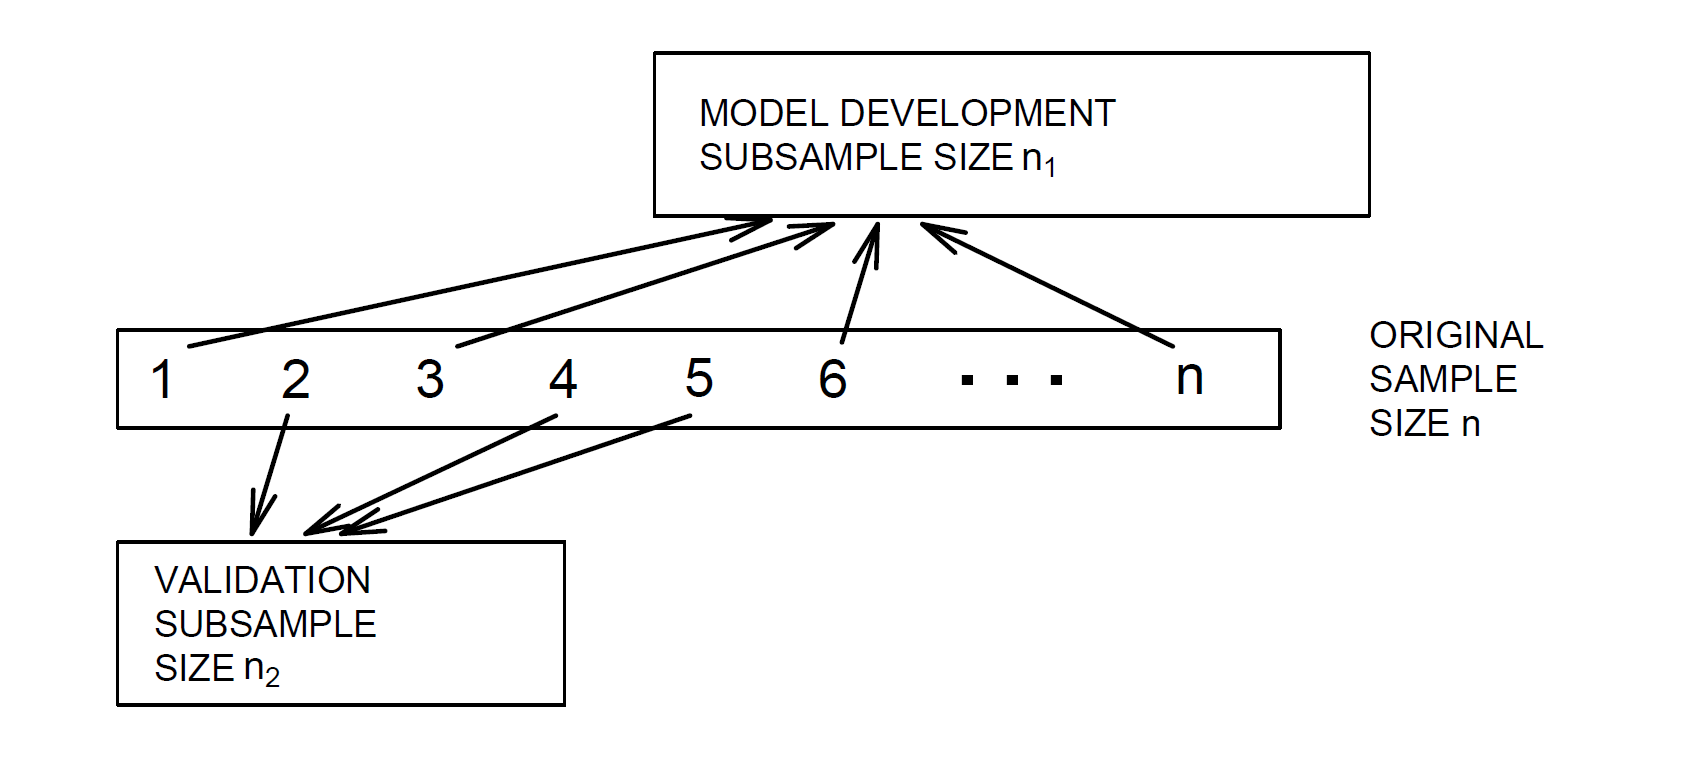
\includegraphics[width=0.8\linewidth]{Figures/F5ModelValidation} 

}

\caption{Model Validation. A data set of size n is randomly split into two subsamples.}\label{fig:ModelValidation}
\end{figure}

Various researchers recommend different proportions for the allocation.
Snee (1977) suggests that data-splitting not be done unless the sample
size is moderately large. The guidelines of Picard and Berk (1990) show
that the greater the number of parameters to be estimated, the greater
the proportion of observations needed for the model development
subsample. As a rule of thumb, for data sets with 100 or fewer
observations, use about 25-35\% of the sample for out-of-sample
validation. For data sets with 500 or more observations, use 50\% of the
sample for out-of-sample validation.

Because of these criticisms, several variants of the basic out-of-sample
validation process are used by analysts. Although there is no
theoretically best procedure, it is widely agreed that model validation
is an important part of confirming the usefulness and appropriateness of
a model.

\subsection{Gini Statistic}\label{gini-statistic}

\subsubsection{The Classic Lorenz Curve}\label{the-classic-lorenz-curve}

In welfare economics, it is common to compare distributions via the
\textbf{Lorenz curve}, developed by Max Otto Lorenz
\citep{lorenz1905methods}. A Lorenz curve is a graph of the proportion
of a population on the horizontal axis and a distribution function of
interest on the vertical axis. It is typically used to represent income
distributions. When the income distribution is perfectly aligned with
the population distribution, the Lorenz curve results in a 45 degree
line that is known as the \textbf{line of equality}. The area between
the Lorenz curve and the line of equality is a measure of the
discrepancy between the income and population distributions. Two times
this area is known as the \textbf{Gini index}, introduced by Corrado
Gini in 1912.

\textbf{Example -- Classic Lorenz Curve.} For an insurance example,
Figure \ref{fig:ClassicLorenz} shows a distribution of insurance losses.
This figure is based on a random sample of 2000 losses. The left-hand
panel shows a right-skewed histogram of losses. The right-hand panel
provides the corresponding Lorenz curve, showing again a skewed
distribution. For example, the arrow marks the point where 60 percent of
the policyholders have 30 percent of losses. The 45 degree line is the
line of equality; if each policyholder has the same loss, then the loss
distribution would be at this line. The Gini index, twice the area
between the Lorenz curve and the 45 degree line, is 37.6 percent for
this data set.

\begin{figure}

{\centering 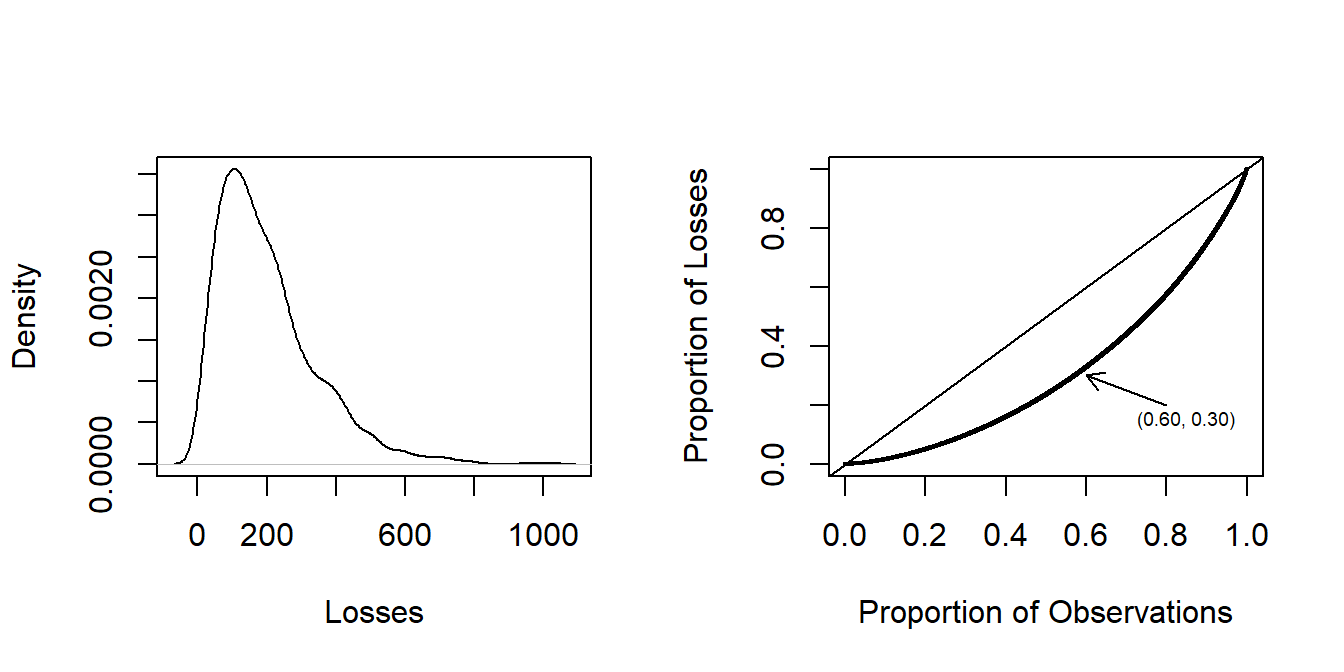
\includegraphics[width=0.9\linewidth]{LossDataAnalytics_files/figure-latex/ClassicLorenz-1} 

}

\caption{Distribution of insurance losses.}\label{fig:ClassicLorenz}
\end{figure}

\subsubsection{Ordered Lorenz Curve and the Gini
Index}\label{ordered-lorenz-curve-and-the-gini-index}

We now introduce a modification of the classic Lorenz curve and Gini
statistic that is useful in insurance applications. Specifically, we
introduce an \emph{ordered} Lorenz curve which is a graph of the
distribution of losses versus premiums, where both losses and premiums
are ordered by relativities. Intuitively, the relativities point towards
aspects of the comparison where there is a mismatch between losses and
premiums. To make the ideas concrete, we first provide some notation. We
will consider \(i=1, \ldots, n\) policies. For the \(i\)th policy, let

\begin{itemize}
\tightlist
\item
  \(y_i\) denote the insurance loss,
\item
  \(\mathbf{x}_i\) be the set of policyholder characteristics known to
  the analyst,
\item
  \(P_i=P(\mathbf{x}_i)\) be the associated premium that is a function
  of \(\mathbf{x}_i\),
\item
  \(S_i = S(\mathbf{x}_i)\) be an insurance score under consideration
  for rate changes, and
\item
  \(R_i = R(\mathbf{x}_i)=S(\mathbf{x}_i)/P(\mathbf{x}_i)\) is the
  relativity, or relative premium.
\end{itemize}

Thus, the set of information used to calculate the ordered Lorenz curve
for the \(i\)th policy is \((y_i, P_i, S_i, R_i)\).

\paragraph{Ordered Lorenz Curve}\label{ordered-lorenz-curve}
\addcontentsline{toc}{paragraph}{Ordered Lorenz Curve}

We now sort the set of policies based on relativities (from smallest to
largest) and compute the premium and loss distributions. Using notation,
the premium distribution is

\begin{equation}\label{E:EmpPremDF}
\hat{F}_P(s) =  \frac{ \sum_{i=1}^n
P(\mathbf{x}_i) \mathrm{I}(R_i \leq s) }{\sum_{i=1}^n P(\mathbf{x}_i)} ,
\end{equation}

and the loss distribution is

\begin{equation}\label{E:EmpLossDF}
\hat{F}_{L}(s) =  \frac{ \sum_{i=1}^n y_i \mathrm{I}(R_i
\leq s) }{\sum_{i=1}^n y_i} ,
\end{equation}

where \(\mathrm{I}(\cdot)\) is the indicator function, returning a 1 if
the event is true and zero otherwise. The graph
\(\left(\hat{F}_P(s),\hat{F}_{L}(s) \right)\) is an \textbf{ordered
Lorenz curve}.

The classic Lorenz curve shows the proportion of policyholders on the
horizontal axis and the loss distribution function on the vertical axis.
The ordered Lorenz curve extends the classical Lorenz curve in two ways,
(1) through the ordering of risks and prices by relativities and (2) by
allowing prices to vary by observation. We summarize the ordered Lorenz
curve in the same way as the classic Lorenz curve using a Gini index,
defined as twice the area between the curve and a 45 degree line. The
analyst seeks ordered Lorenz curves that approach passing through the
southeast corner (1,0); these have greater separation between the loss
and premium distributions and therefore larger Gini indices.

\textbf{Example -- Loss Distribution.}

Suppose we have \(n=5\) policyholders with experience as:

\begin{longtable}[]{@{}lcllllll@{}}
\toprule
Variable & \(i\) & 1 & 2 & 3 & 4 & 5 & Sum\tabularnewline
\midrule
\endhead
Loss & \(y_i\) & 5 & 5 & 5 & 4 & 6 & 25\tabularnewline
Premium & \(P(\mathbf{x}_i)\) & 4 & 2 & 6 & 5 & 8 & 25\tabularnewline
\begin{minipage}[t]{0.12\columnwidth}\raggedright\strut
Relativity\strut
\end{minipage} & \begin{minipage}[t]{0.12\columnwidth}\centering\strut
\(R(\mathbf{x}_i)\)\strut
\end{minipage} & \begin{minipage}[t]{0.12\columnwidth}\raggedright\strut
5\strut
\end{minipage} & \begin{minipage}[t]{0.12\columnwidth}\raggedright\strut
4\strut
\end{minipage} & \begin{minipage}[t]{0.12\columnwidth}\raggedright\strut
3\strut
\end{minipage} & \begin{minipage}[t]{0.12\columnwidth}\raggedright\strut
2\strut
\end{minipage} & \begin{minipage}[t]{0.12\columnwidth}\raggedright\strut
1\strut
\end{minipage} & \begin{minipage}[t]{0.12\columnwidth}\raggedright\strut
\strut
\end{minipage}\tabularnewline
\bottomrule
\end{longtable}

Determine the Lorenz curve and the ordered Lorenz curve.

Show Example Solution

\hypertarget{toggleLorenz}{}
\begin{figure}

{\centering 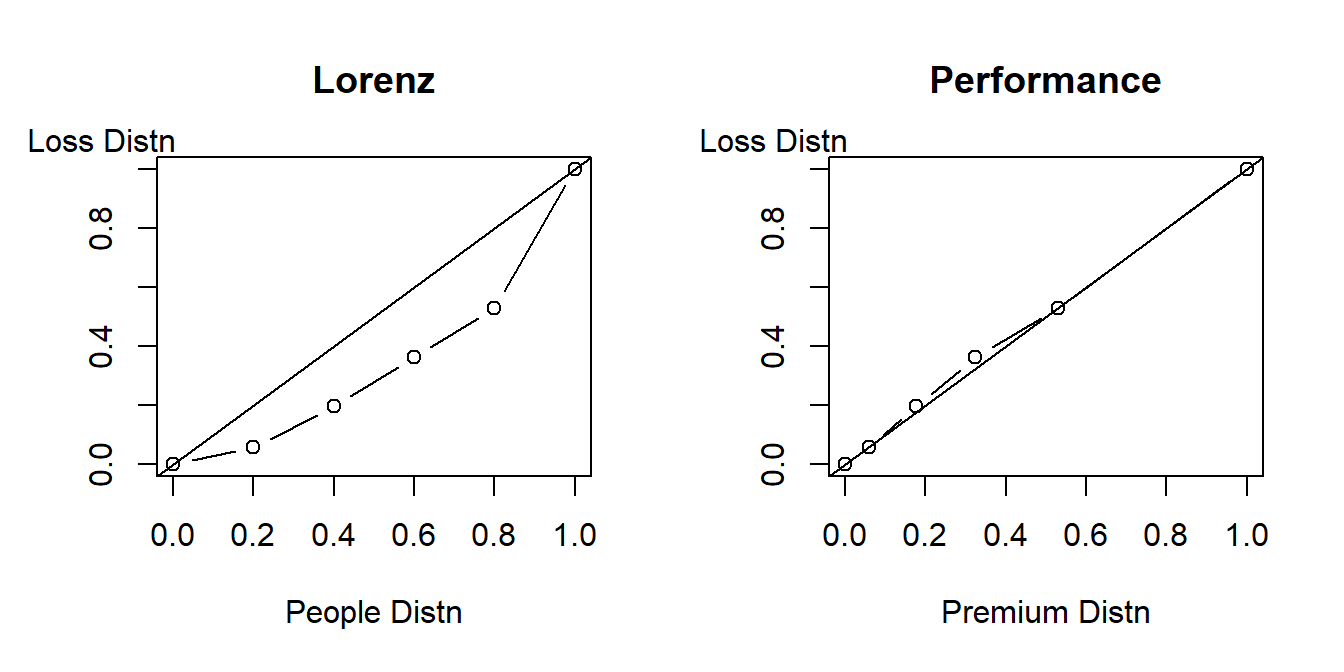
\includegraphics[width=0.9\linewidth]{LossDataAnalytics_files/figure-latex/LorenzVsOrdered-1} 

}

\caption{Lorenz versus Ordered Lorenz Curve}\label{fig:LorenzVsOrdered}
\end{figure}

Figure \ref{fig:LorenzVsOrdered} compares the Lorenz curve to the
ordered version based on this data. The left-hand panel shows the Lorenz
curve. The horizontal axis is the cumulative proportion of policyholders
(0, 0.2, 0.4, and so forth) and the vertical axis is the cumulative
proportion of losses (0, 4/25, 9/25, and so forth). This figure shows
little separation between the distributions of losses and policyholders.

The right-hand panel shows the ordered Lorenz curve. Because
observations are sorted by relativities, the first point after the
origin (reading from left to right) is (8/25, 6/25). The second point is
(13/25, 10/25), with the pattern continuing. For the ordered Lorenz
curve, the horizontal axis uses premium weights, the vertical axis uses
loss weights, and both axes are ordered by relativities. From the
figure, we see that there is greater separation between losses and
premiums when viewed through this relativity.

\paragraph{Gini Index}\label{gini-index}
\addcontentsline{toc}{paragraph}{Gini Index}

Specifically, the Gini index can be calculated as follows. Suppose that
the empirical ordered Lorenz curve is given by
\(\{ (a_0=0, b_0=0), (a_1, b_1), \ldots,\) \((a_n=1, b_n=1) \}\) for a
sample of \(n\) observations. Here, we use \(a_j = \hat{F}_P(R_j)\) and
\(b_j = \hat{F}_{L}(R_j)\). Then, the empirical Gini index is

\begin{eqnarray}\label{E:GiniDefn}
\widehat{Gini} &=&  2\sum_{j=0}^{n-1} (a_{j+1} - a_j) \left \{
\frac{a_{j+1}+a_j}{2} - \frac{b_{j+1}+b_j}{2} \right\} \nonumber \\
&=& 1 - \sum_{j=0}^{n-1} (a_{j+1} - a_j) (b_{j+1}+b_j) .
\end{eqnarray}

\textbf{Example -- Loss Distribution: Continued.} In the figure, the
Gini index for the left-hand panel is 5.6\%. In contrast, the Gini index
for the right-hand panel is 14.9\%. \(~~\Box\)

\subsubsection{Out-of-Sample
Validation}\label{out-of-sample-validation-1}

The Gini statistics based on an ordered Lorenz curve can be used for
out-of-sample validation. The procedure follows:

\begin{enumerate}
\def\labelenumi{\arabic{enumi}.}
\tightlist
\item
  Use an in-sample data set to estimate several competing models.
\item
  Designate an out-of-sample, or validation, data set of the form
  \(\{(y_i, \mathbf{x}_i), i=1,\ldots,n\}\).
\item
  Establish one of the models as the base model. Use this estimated
  model and explanatory variables from the validation sample to form
  premiums of the form \(P(\mathbf{x}_i))\).
\item
  Use an estimated competing model and validation sample explanatory
  variables to form scores of the form \(S(\mathbf{x}_i))\).
\item
  From the premiums and scores, develop relativities
  \(R_i =S(\mathbf{x}_i)/P(\mathbf{x}_i)\).
\item
  Use the validation sample outcomes \(y_i\) to compute the Gini
  statistic.
\end{enumerate}

\textbf{Example -- Out-of-Sample Validation.}

Suppose that we have experience from 25 states. For each state, we have
available 500 observations that can be used to predict future losses.
For this illustration, we have generated losses using a gamma
distrbution with common shape parameter equal to 5 and a scale parameter
that varies by state, from a low of 20 to 66.

Determine the ordered Lorenz curve and the corresponding Gini statistic
to compare the two rate procedures.

Show Example Solution

\hypertarget{toggleExampleLor}{}
For our base premium, we simply use the maximum likelihood estimate
assuming a common distribution among all states. For the gamma
distribution, this turns out to be simply the average which for our
simulation is \textbf{P}=219.96. You can think of this common premium as
based on a \emph{community rating} principle. As an alternative, we use
averages that are state-specific. Because this illustration uses means
that vary by states, we anticipate this alternative rating procedure to
be preferred to the community rating procedure. (Recall for the gamma
distribution that the mean equals the shape times the scale or, 5 times
the scale parameter, for our example.)

Out of sample claims were generated from the same gamma distribution,
with 200 observations for each state. In the following, we have the
ordered Lorenz curve.

\begin{figure}

{\centering 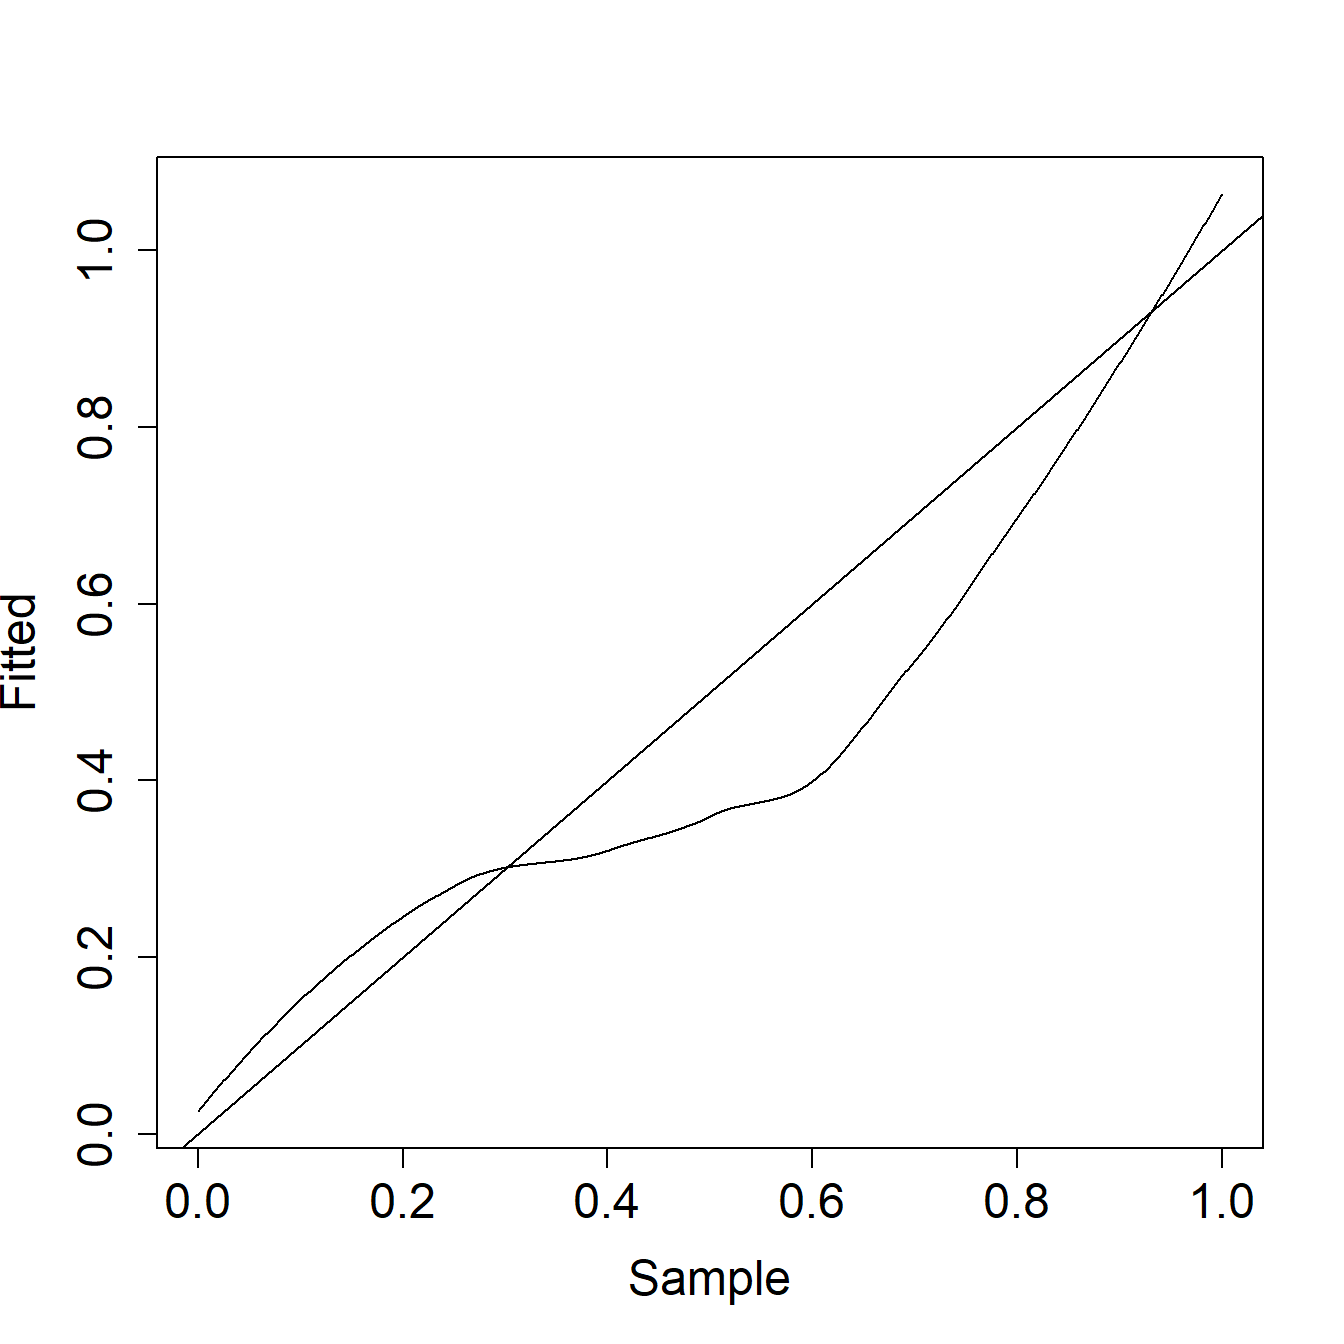
\includegraphics[width=0.5\linewidth]{LossDataAnalytics_files/figure-latex/unnamed-chunk-7-1} 

}

\end{figure}

For these data, the Gini index is 0.187 with a standard error equal to
0.00381.

\paragraph{Discussion}\label{discussion}
\addcontentsline{toc}{paragraph}{Discussion}

In insurance claims modeling, standard out-of-sample validation measures
are not the most informative due to the high proportions of zeros
(corresponding to no claim) and the skewed fat-tailed distribution of
the positive values. The Gini index can be motivated by the economics of
insurance. Intuitively, the Gini index measures the negative covariance
between a policy's ``profit'' (\(P-y\), premium minus loss) and the rank
of the relativity (\textbf{R}, score divided by premium). That is, the
close approximation

\[\widehat{Gini} \approx - \frac{2}{n} \widehat{Cov} \left( (P-y), rank(R) \right) .\]
This observation leads an insurer to seek an ordering that produces to a
large Gini index. Thus, the Gini index and associated ordered Lorenz
curve are useful for identifying profitable blocks of insurance
business.

Unlike classical measures of association, the Gini index assumes that a
premium base \textbf{P} is currently in place and seeks to assess
vulnerabilities of this structure. This approach is more akin to
hypothesis testing (when compared to goodness of fit) where one
identifies a ``null hypothesis'' as the current state of the world and
uses decision-making criteria/statistics to compare this with an
``alternative hypothesis.''

The insurance version of the Gini statistic was developed by
\citep{frees2011summarizing} and \citep{frees2014insurance} where you
can find formulas for the standard errors and other additional
background information.

\section{Modified Data}\label{S:ModifiedData}

In this section, you learn how to:

\begin{itemize}
\tightlist
\item
  Describe grouped, censored, and truncated data
\item
  Estimate parametric distributions based on grouped, censored, and
  truncated data
\item
  Estimate distributions nonparametrically based on grouped, censored,
  and truncated data
\end{itemize}

\subsection{Parametric Estimation using Modified
Data}\label{parametric-estimation-using-modified-data}

Basic theory and many applications are based on \emph{individual}
observations that are ``\emph{complete}'' and ``\emph{unmodified},'' as
we have seen in the previous section. Chapter 3 introduced the concept
of observations that are ``\emph{modified}'' due to two common types of
limitations: \textbf{censoring} and \textbf{truncation}. This section
will address parametric estmation methods for three alternatives to
individual, complete, and unmodified data: \textbf{interval-censored}
data available only in groups, data that are limited or
\textbf{censored}, and data that may not be observed due to
\textbf{truncation}.

\subsubsection{Parametric Estimation using Grouped
Data}\label{S:GroupedData}

Consider a sample of size \(n\) observed from the distribution
\(F(\cdot)\), but in groups so that we only know the group into which
each observation fell, but not the exact value. This is referred to as
\textbf{grouped} or \textbf{interval-censored} data. For example, we may
be looking at two successive years of annual employee records. People
employed in the first year but not the second have left sometime during
the year. With an exact departure date (individual data), we could
compute the amount of time that they were with the firm. Without the
departure date (grouped data), we only know that they departed sometime
during a year-long interval.

Formalizing this idea, suppose there are \(k\) groups or intervals
delimited by boundaries \(c_0 < c_1< \cdots < c_k\). For each
observation, we only observe the interval into which it fell (e.g.
\((c_{j-1}, c_j)\)), not the exact value. Thus, we only know the number
of observations in each interval. The constants
\(\{c_0 < c_1 < \cdots < c_k\}\) form some partition of the domain of
\(F(\cdot)\). Then the probability of an observation \(X_i\) falling in
the \(j\)th interval is \[\Pr\left(X
_i \in (c_{j-1}, c_j]\right) = F(c_j) - F(c_{j-1}).\]

The corresponding probability mass function for an observation is
\[\begin{aligned}
f(x) &=
\begin{cases}
F(c_1) - F(c_{0}) &   \text{if }\ x \in (c_{0}, c_1]\\
\vdots & \vdots \\
F(c_k) - F(c_{k-1}) &   \text{if }\ x \in (c_{k-1}, c_k]\\
\end{cases} \\
&= \prod_{j=1}^k \left\{F(c_j) - F(c_{j-1})\right\}^{I(x \in (c_{j-1}, c_j])}
\end{aligned}\]

Now, define \(n_j\) to be the number of observations that fall in the
\(j\)th interval, \((c_{j-1}, c_j]\). Thus, the likelihood function
(with respect to the parameter(s) \(\theta\)) is \[\begin{aligned}
\mathcal{L}(\theta) = \prod_{j=1}^n f(x_i) = \prod_{j=1}^k \left\{F(c_j) - F(c_{j-1})\right\}^{n_j}
\end{aligned}\]

And the log-likelihood function is \[\begin{aligned}
L(\theta) = \ln \mathcal{L}(\theta) = \ln \prod_{j=1}^n f(x_i) = \sum_{j=1}^k n_j \ln \left\{F(c_j) - F(c_{j-1})\right\}
\end{aligned}\]

Maximizing the likelihood function (or equivalently, maximizing the
log-likelihood function) would then produce the maximum likelihood
estimates for grouped data.

\subsubsection{Censored Data}\label{censored-data}

\textbf{Censoring} occurs when we observe only a limited value of an
observation. The most common form is \textbf{right-censoring}, in which
we record the smaller of the ``true'' dependent variable and a censoring
variable. Using notation, let \(X\) represent an outcome of interest,
such as the loss due to an insured event. Let \(C_U\) denote the
censoring time, such as \(C_U=5\). With right-censored observations, we
observe \(X\) if it is below censoring point \(C_U\); otherwise if \(X\)
is higher than the censoring point, we only observe the censored
\(C_U\). Therefore, we record \(X_U^{\ast}= \min(X, C_U)\). We also
observe whether or not censoring has occurred. Let
\(\delta_U= \mathrm{I}(X \geq C_U)\) be a binary variable that is 1 if
censoring occurs, \(y \geq C_U\), and 0 otherwise.

For example, \(C_U\) may represent the upper limit of coverage of an
insurance policy. The loss may exceed the amount \(C_U\), but the
insurer only has \(C_U\) in its records as the amount paid out and does
not have the amount of the actual loss \(X\) in its records.

Similarly, with \textbf{left-censoring}, we only observe \(X\) if \(X\)
is above censoring point (e.g.~time or loss amount) \(C_L\); otherwise
we observe \(C_L\). Thus, we record \(X_L^{\ast}= \max(X, C_L)\) along
with the censoring indicator \(\delta_L= \mathrm{I}(X \leq C_L)\).

For example, suppose a reinsurer will cover insurer losses greater than
\(C_L\). Let \(Y = X_L^{\ast} - C_L\) represent the amount that the
\emph{reinsurer} is responsible for. If the policyholder loss
\(X < C_L\), then the insurer will pay the entire claim and \(Y =0\), no
loss for the reinsurer. If the loss \(X \ge C_L\), then \(Y = X-C_L\)
represents the reinsurer's retained claims. If a loss occurs, the
reinsurer knows the actual amount if it exceeds the limit \(C_L\),
otherwise it only knows that it had a loss of \(0\).

As another example of a left-censored observation, suppose we are
conducting a study and interviewing a person about an event in the past.
The subject may recall that the event occurred before \(C_L\), but not
the exact date.

\subsubsection{Truncated Data}\label{truncated-data}

We just saw that censored observations are still available for study,
although in a limited form. In contrast, \textbf{truncated} outcomes are
a type of missing data. An outcome is potentially truncated when the
availability of an observation depends on the outcome.

In insurance, it is common for observations to be
\textbf{left-truncated} at \(C_L\) when tfhe amount is \[\begin{aligned}
Y &=
\left\{
\begin{array}{ll}
\text{we do not observe }X & X < C_L \\
X- C_L & X \geq C_L.
\end{array}
\right.\end{aligned}\]

In other words, if \(X\) is less than the threshold \(C_L\), then it is
not observed. FOr example, \(C_L\) may represent the deductible
associated with an insurance coverage. If the insured loss is less than
the deductible, then the insurer does not observe or record the loss at
all. If the loss exceeds the deductible, then the excess \(X-C_L\) is
the claim that the insurer covers.

Similarly for \textbf{right-truncated} data, if \(X\) exceeds a
threshold \(C_U\), then it is not observed. In this case, the amount is
\[\begin{aligned}
Y &=
\left\{
\begin{array}{ll}
X & X < C_U \\
\text{we do not observe }X & X \geq C_U.
\end{array}
\right.\end{aligned}\]

Classic examples of truncation from the right include \(X\) as a measure
of distance to a star. When the distance exceeds a certain level
\(C_U\), the star is no longer observable.

Figure \ref{fig:CensorTrunc} compares truncated and censored
observations. Values of \(X\) that are greater than the ``upper''
censoring limit \(C_U\) are not observed at all (right-censored), while
values of \(X\) that are smaller than the ``lower'' truncation limit
\(C_L\) are observed, but observed as \(C_L\) rather than the actual
value of \(X\) (left-truncated).

\begin{figure}

{\centering 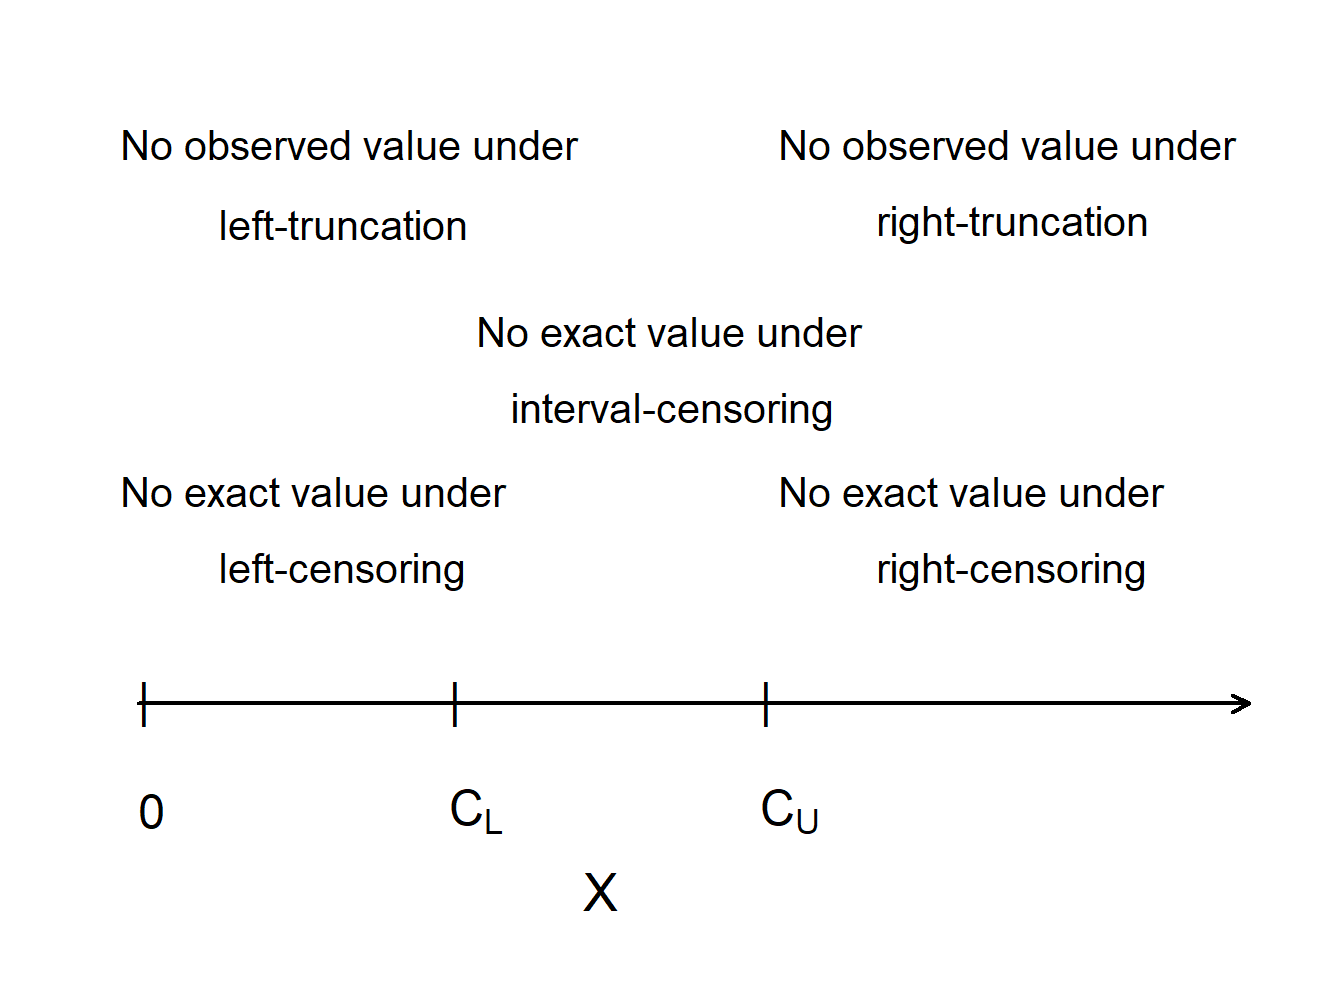
\includegraphics[width=0.6\linewidth]{LossDataAnalytics_files/figure-latex/CensorTrunc-1} 

}

\caption{Figure 8: Censoring and Truncation}\label{fig:CensorTrunc}
\end{figure}

\begin{center}\rule{0.5\linewidth}{\linethickness}\end{center}

Show Example

\hypertarget{toggleExampleMort}{}
\textbf{Example -- Mortality Study.} Suppose that you are conducting a
two-year study of mortality of high-risk subjects, beginning January 1,
2010 and finishing January 1, 2012. Figure \ref{fig:Mortality}
graphically portrays the six types of subjects recruited. For each
subject, the beginning of the arrow represents that the the subject was
recruited and the arrow end represents the event time. Thus, the arrow
represents exposure time.

\begin{figure}

{\centering 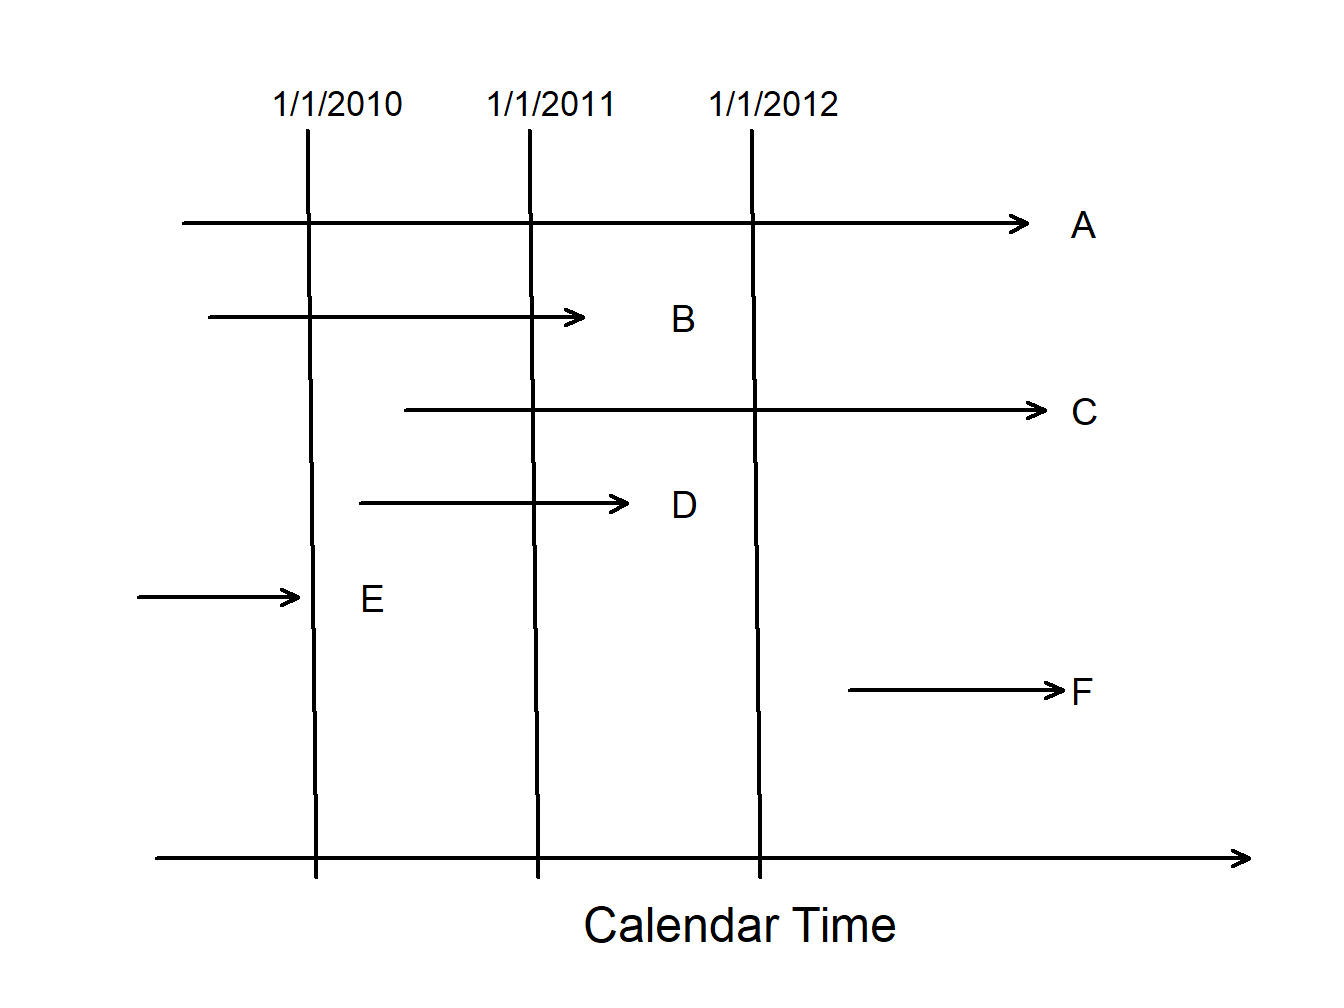
\includegraphics[width=0.6\linewidth]{LossDataAnalytics_files/figure-latex/Mortality-1} 

}

\caption{Figure 9: Timeline for Several Subjects on Test in a Mortality Study}\label{fig:Mortality}
\end{figure}

\begin{itemize}
\tightlist
\item
  \textbf{Type A - Right-censored.} This subject is alive at the
  beginning and the end of the study. Because the time of death is not
  known by the end of the study, it is right-censored. Most subjects are
  Type A.
\item
  \textbf{Type B - Complete} information is available for a type B
  subject. The subject is alive at the beginning of the study and the
  death occurs within the observation period.
\item
  \textbf{Type C - Right-censored and left-truncated.} A type C subject
  is right-censored, in that death occurs after the observation period.
  However, the subject entered after the start of the study and is said
  to have a \emph{delayed entry time}. Because the subject would not
  have been observed had death occurred before entry, it is
  left-truncated.
\item
  \textbf{Type D - Left-truncated.} A type D subject also has delayed
  entry. Because death occurs within the observation period, this
  subject is not right censored.
\item
  \textbf{Type E - Left-truncated.} A type E subject is not included in
  the study because death occurs prior to the observation period.
\item
  \textbf{Type F - Right-truncated.} Similarly, a type F subject is not
  included because the entry time occurs after the observation period.
\end{itemize}

\begin{center}\rule{0.5\linewidth}{\linethickness}\end{center}

To summarize, for outcome \(X\) and constants \(C_L\) and \(C_U\),

\begin{longtable}[]{@{}ccc@{}}
\toprule
Limitation Type & Limited Variable & Censoring
Information\tabularnewline
\midrule
\endhead
right censoring & \(X_U^{\ast}= \min(X, C_U)\) &
\(\delta_U= \mathrm{I}(X \geq C_U)\)\tabularnewline
left censoring & \(X_L^{\ast}= \max(y, C_L)\) &
\(\delta_L= \mathrm{I}(X \leq C_L)\)\tabularnewline
\begin{minipage}[t]{0.32\columnwidth}\centering\strut
interval censoring\strut
\end{minipage} & \begin{minipage}[t]{0.32\columnwidth}\centering\strut
\strut
\end{minipage} & \begin{minipage}[t]{0.32\columnwidth}\centering\strut
\strut
\end{minipage}\tabularnewline
right truncation & \(X\) & observe \(X\) if \(X < C_U\)\tabularnewline
left truncation & \(X\) & observe \(X\) if \(X < C_L\)\tabularnewline
\bottomrule
\end{longtable}

\subsubsection{Parametric Estimation using Censored and Truncated
Data}\label{parametric-estimation-using-censored-and-truncated-data}

For simplicity, we assume fixed censoring times and a continuous outcome
\(X\). To begin, consider the case of right-censored data where we
record \(X_U^{\ast}= \min(X, C_U)\) and censoring indicator
\(\delta_U= \mathrm{I}(X \geq C_U)\). If censoring occurs so that
\(\delta_U=1\), then \(X \geq C_U\) and the likelihood is
\(\Pr(X \geq C_U) = 1-F(C_U)\). If censoring does not occur so that
\(\delta_U=0\), then \(X < C_U\) and the likelihood is \(f(x)\).
Summarizing, we have the likelihood of a single observation as

\[\begin{aligned}
\left\{
\begin{array}{ll}
f(x) & \text{if } \delta = 0 \\
1-F(C_U) & \text{if }\delta=1
\end{array}
\right. = \left( f(x)\right)^{1-\delta} \left(1-F(C_U)\right)^{\delta} .
\end{aligned}\]

The right-hand expression allows us to present the likelihood more
compactly. Now, for an \emph{iid} sample of size \(n\),
\(\{ (x_{U1},\delta_1), \ldots,(x_{Un}, \delta_n) \}\), the likelihood
is

\[\mathcal{L}(\theta) = \prod_{i=1}^n \left( f(x_i)\right)^{1-\delta_i} \left(1-F(C_{Ui})\right)^{\delta_i} = \prod_{\delta_i=0} f(x_i) \prod_{\delta_i=1} \{1-F(C_{Ui})\},\]

with potential censoring times \(\{ C_{U1}, \ldots,C_{Un} \}\). Here,
the notation ``\(\prod_{\delta_i=0}\)'' means to take the product over
uncensored observations, and similarly for ``\(\prod_{\delta_i=1}\).''

On the other hand, truncated data are handled in likelihood inference
via conditional probabilities. Specifically, we adjust the likelihood
contribution by dividing by the probability that the variable was
observed. To summarize, we have the following contributions to the
likelihood function for six types of outcomes:

\[\begin{array}{lc}
\hline
\text{Outcome} & \text{Likelihood Contribution} \\
\hline 
\text{exact value} & f(x) \\
\text{right-censoring} & 1-F(C_U) \\
\text{left-censoring} & F(C_L) \\
\text{right-truncation} & f(x)/F(C_U) \\
\text{left-truncation} & f(x)/(1-F(C_L)) \\
\text{interval-censoring} & F(C_U)-F(C_L) \\
\hline
\end{array}\]

For known outcomes and censored data, the likelihood is
\[\mathcal{L}(\theta) = \prod_{E} f(x_i) \prod_{R} \{1-F(C_{Ui})\} \prod_{L}
F(C_{Li}) \prod_{I} (F(C_{Ui})-F(C_{Li})),\] where ``\(\prod_{E}\)'' is
the product over observations with \emph{E}xact values, and similarly
for \emph{R}ight-, \emph{L}eft- and \emph{I}nterval-censoring.

For right-censored and left-truncated data, the likelihood is
\[\mathcal{L}(\theta) = \prod_{E} \frac{f(x_i)}{1-F(C_{Li})} \prod_{R} \frac{1-F(C_{Ui})}{1-F(C_{Li})},\]
and similarly for other combinations. To get further insights, consider
the following.

\begin{center}\rule{0.5\linewidth}{\linethickness}\end{center}

Show Example

\hypertarget{toggleExampleEXP}{}
\textbf{Special Case: Exponential Distribution.} Consider data that are
right-censored and left-truncated, with random variables \(X_i\) that
are exponentially distributed with mean \(\theta\). With these
specifications, recall that \(f(x) = \theta^{-1} \exp(-x/\theta)\) and
\(F(x) = 1-\exp(-x/\theta)\).

For this special case, the log-likelihood is

\[\begin{aligned}
L(\theta) &= \sum_{E} \left\{ \ln f(x_i) - \ln (1-F(C_{Li})) \right\} + \sum_{R}\left\{ \ln (1-F(C_{Ui}))- \ln (1-\mathrm{F}(C_{Li})) \right\}\\
&= \sum_{E} (-\ln \theta -(x_i-C_{Li})/\theta ) -\sum_{R} (C_{Ui}-C_{Li})/\theta .
\end{aligned}\]

To simplify the notation, define
\(\delta_i = \mathrm{I}(X_i \geq C_{Ui})\) to be a binary variable that
indicates right-censoring. Let
\(X_i^{\ast \ast} = \min(X_i, C_{Ui}) - C_{Li}\) be the amount that the
observed variable exceeds the lower truncation limit. With this, the
log-likelihood is

\begin{equation} 
  L(\theta) =  - \sum_{i=1}^n ((1-\delta_i) \ln \theta + \frac{x_i^{\ast \ast}}{\theta})
  \label{eq:EXPloglik}
\end{equation}

Taking derivatives with respect to the parameter \(\theta\) and setting
it equal to zero yields the maximum likelihood estimator

\[\widehat{\theta}  = \frac{1}{n_u} \sum_{i=1}^n  x_i^{\ast \ast},\]

where \(n_u = \sum_i (1-\delta_i)\) is the number of uncensored
observations.

\begin{center}\rule{0.5\linewidth}{\linethickness}\end{center}

\textbf{Exercise -- Exam C Question 44.} You are given:

\begin{enumerate}
\def\labelenumi{(\roman{enumi})}
\tightlist
\item
  Losses follow an exponential distribution with mean \(\theta\).
\item
  A random sample of 20 losses is distributed as follows:
\end{enumerate}

\[\begin{array}{l|c}
\hline
\text{Loss Range} & \text{Frequency} \\
\hline 
[0,1000] & 7 \\
(1000,2000] & 6 \\
(2000,\infty) & 7 \\
\hline
\end{array}\]

Calculate the maximum likelihood estimate of \(\theta\).

Show Solution

\hypertarget{toggleExamC44}{}
\emph{Solution:} \[\begin{aligned}
\mathcal{L}(\theta) &= F(1000)^7[F(2000)-F(1000)]^6[1-F(2000)]^7 \\
&= (1-e^{-1000/\theta})^7(e^{-1000/\theta} - e^{-2000/\theta})^6(e^{-2000/\theta})^7 \\
&= (1-p)^7(p-p^2)^6(p^2)^7 \\
&= p^{20}(1-p)^{13}
\end{aligned}\]

where \(p=e^{-1000/\theta}\). Maximizing this expression with respect to
\(p\) is equivalent to maximizing the likelihood with respect to
\(\theta\). The maximum occurs at \(p=\frac{20}{33}\) and so
\(\hat{\theta}=\frac{-1000}{\ln(20/33)}= 1996.90\).

\begin{center}\rule{0.5\linewidth}{\linethickness}\end{center}

\textbf{Exercise -- Exam C Question 152.} You are given:

\begin{enumerate}
\def\labelenumi{(\roman{enumi})}
\tightlist
\item
  A sample of losses is: 600 700 900
\item
  No information is available about losses of 500 or less.
\item
  Losses are assumed to follow an exponential distribution with mean
  \(\theta\).
\end{enumerate}

Calculate the maximum likelihood estimate of \(\theta\).

Show Solution

\hypertarget{toggleExamC152}{}
\emph{Solution:} These observations are truncated at 500. The
contribution of each observation to the likelihood function is
\[\frac{f(x)}{1-F(500)} = \frac{\theta^{-1}e^{-x/\theta}}{e^{-500/\theta}}\]

Then the likelihood function is

\[\mathcal{L}(\theta)= \frac{\theta^{-1} e^{-600/\theta} \theta^{-1} e^{-700/\theta} \theta^{-1} e^{-900/\theta}}{(e^{-500/\theta})^3} = \theta^{-3}e^{-700/\theta}\]

The log-likelihood is

\[L(\theta) = \ln\mathcal{L}(\theta) = -3\ln \theta - 700\theta^{-1}\]

Maximizing this expression by setting the derivative with respect to
\(\theta\) equal to 0, we have

\[L'(\theta) = -3\theta^{-1} + 700\theta^{-2} = 0 \ \Rightarrow \ \hat{\theta} = \frac{700}{3} = 233.33\]

\begin{center}\rule{0.5\linewidth}{\linethickness}\end{center}

\textbf{Course 4: Fall 2000, Question 22.} You are given the following
information about a random sample:

\begin{enumerate}
\def\labelenumi{(\roman{enumi})}
\tightlist
\item
  The sample size equals five.
\item
  The sample is from a Weibull distribution with \(\tau=2\).
\item
  Two of the sample observations are known to exceed 50, and the
  remaining three observations are 20, 30, and 45.
\end{enumerate}

Calculate the maximum likelihood estimate of \(\theta\).

Show Solution

\hypertarget{toggleF00Q22}{}
\emph{Solution:} The likelihood function is

\[\begin{aligned} 
\mathcal{L}(\theta) &= f(20) f(30) f(45) [1-F(50)]^2 \\
&= \frac{2(20/\theta)^2 e^{-(20/\theta)^2}}{20} \frac{2(30/\theta)^2 e^{-(30/\theta)^2}}{30} \frac{2(45/\theta)^2 e^{-(45/\theta)^2}}{45}(e^{-(50/\theta)^2})^2 \\
&\propto \frac{1}{\theta^6} e^{-8325/\theta^2}
\end{aligned}\]

The natural logarithm of the above expression is
\(-6\ln\theta - \frac{8325}{\theta^2}\). Maximizing this expression by
setting its derivative to 0, we get

\[\frac{-6}{\theta} + \frac{16650}{\theta^3} = 0 \ \Rightarrow \ \hat{\theta} = \left(\frac{16650}{6}\right)^{\frac{1}{2}} = 52.6783\]

\begin{center}\rule{0.5\linewidth}{\linethickness}\end{center}

\subsection{Nonparametric Estimation using Modified
Data}\label{nonparametric-estimation-using-modified-data}

Nonparametric estimators provide useful benchmarks, so it is helpful to
understand the estimation procedures for grouped, censored, and
truncated data.

\subsubsection{Grouped Data}\label{grouped-data}

As we have seen in Section \ref{S:GroupedData}, observations may be
grouped (also referred to as interval censored) in the sense that we
only observe them as belonging in one of \(k\) intervals of the form
\((c_{j-1}, c_j]\), for \(j=1, \ldots, k\). At the boundaries, the
empirical distribution function is defined in the usual way:
\[F_n(c_j) = \frac{\text{number of observations } \le c_j}{n}\]

For other values of \(x \in (c_{j-1}, c_j)\), we can estimate the
distribution function with the \textbf{ogive} estimator, which linearly
interpolates between \(F_n(c_{j-1})\) and \(F_n(c_j)\), i.e.~the values
of the boundaries \(F_n(c_{j-1}\) and \(F_n(c_j)\) are connected with a
straight line. This can formally be expressed as
\[F_n(x) = \frac{c_j-x}{c_j-c_{j-1}} F_n(c_{j-1}) + \frac{x-c_{j-1}}{c_j-c_{j-1}} F_n(c_j) \ \ \ \text{for } c_{j-1} \le x < c_j\]

The corresponding density is
\[f_n(x) = F^{\prime}_n(x) = \frac{F_n(c_j)-F_n(c_{j-1})}{c_j - c_{j-1}} \ \ \  \text{for } c_{j-1} \le x < c_j .\]

\begin{center}\rule{0.5\linewidth}{\linethickness}\end{center}

\textbf{Exercise -- Exam C Question 195.} You are given the following
information regarding claim sizes for 100 claims:

Using the ogive, calculate the estimate of the probability that a
randomly chosen claim is between 2000 and 6000.

Show Solution

\hypertarget{toggleExamC195}{}
\emph{Solution:} At the boundaries, the empirical distribution function
is defined in the usual way, so we have
\[F_{100}(1000) = 0.16, \ F_{100}(3000)=0.38, \ F_{100}(5000)=0.63, \ F_{100}(10000)=0.81\]
For other claim sizes, the ogive estimator linearly interpolates between
these values:
\[F_{100}(2000) = 0.5F_{100}(1000) + 0.5F_{100}(3000) = 0.5(0.16)+0.5(0.38)=0.27\]
\[F_{100}(6000)=0.8F_{100}(5000)+0.2F_{100}(10000) = 0.8(0.63)+0.2(0.81)=0.666\]
Thus, the probability that a claim is between 2000 and 6000 is
\(F_{100}(6000) - F_{100}(2000) = 0.666-0.27 = 0.396\).

\begin{center}\rule{0.5\linewidth}{\linethickness}\end{center}

\subsubsection{Right-Censored, Left-Truncated Empirical Distribution
Functions}\label{right-censored-left-truncated-empirical-distribution-functions}

It can be useful to calibrate parametric likelihood methods with
nonparametric methods that do not rely on a parametric form of the
distribution. The product-limit estimator due to \citep{kaplan1958} is a
well-known estimator of the distribution in the presence of censoring.

To introduce this estimator, consider the case of right-censored,
left-truncated data. For each observation \(i\), let \(d_i\) be the
lower truncation limit (0 if no truncation) and let \(u_i\) be the upper
censoring limit (\(=\infty\) if no censoring). Thus, the recorded value
(if it is greater than \(d_i\)) is \(x_i\) in the case of no censoring
and \(u_i\) if there is censoring. Let \(t_{1} <\cdots< t_{k}\) be \(k\)
distinct distinct time points at which an event of interest (such as
uncensored losses) occurs, and let \(s_j\) be the number of recorded
events \(x_i\)'s at time point \(t_{j}\). The corresponding \textbf{risk
set} is the number of observations that are active (have not experienced
a loss) at an instant \emph{just prior to} \(t_{j}\), denoted
\(R_j = \sum_{i=1}^n I(x_i \geq t_{j}) + \sum_{i=1}^n I(u_i \geq t_{j}) - \sum_{i=1}^n I(d_i \geq t_{j})\).

With this notation, the \textbf{product-limit estimator} of the
distribution function is

\[\begin{aligned}
\hat{F}(x) &=
\left\{
\begin{array}{ll}
0 & x<t_{1} \\
1-\prod_{j:t_{j} \leq x}\left( 1-\frac{s_j}{R_{j}}\right) & x \geq t_{1} .
\end{array}
\right.\end{aligned}\]

\citep{greenwood1926} derived the formula for the estimated variance of
the product-limit estimator to be

\[\widehat{Var}(\hat{F}(x)) = (\hat{F}(x))^{2} \sum _{j:t_{j} \leq x} \dfrac{s_j}{R_{j}(R_{j}-s_j)}.\]

\texttt{R}`s \texttt{survfit} method takes a survival data object and
creates a new object containing the Kaplan-Meier estimate of the
survival function along with confidence intervals. The Kaplan-Meier
method (\texttt{type=\textquotesingle{}kaplan-meier\textquotesingle{}})
is used by default to construct an estimate of the survival curve. The
resulting discrete survival function has point masses at the observed
event times (discharge dates) \(t_j\), where the probability of an event
given survival to that duration is estimated as the number of observed
events at the duration \(s_j\) divided by the number of subjects exposed
or 'at-risk' just prior to the event duration \(R_j\).

Two alternate types of estimation are also available for the
\texttt{survfit} method. The alternative
(\texttt{type=\textquotesingle{}fh2\textquotesingle{}}) handles ties, in
essence, by assuming that multiple events at the same duration occur in
some arbitrary order. Another alternative
(\texttt{type=\textquotesingle{}fleming-harrington\textquotesingle{}})
uses the Nelson-Äalen (see \citep{aalen1978}) estimate of the
\textbf{cumulative hazard function} to obtain an estimate of the
survival function. The estimated cumulative hazard \(\hat{H}(x)\) starts
at zero and is incremented at each observed event duration \(t_j\) by
the number of events \(s_j\) divided by the number at risk \(R_j\). With
the same notation as above, the \textbf{Nelson-Äalen} estimator of the
distribution function is

\[\begin{aligned}
\hat{F}(x) &=
\left\{
\begin{array}{ll}
0 & x<t_{1} \\
1- \exp \left(\sum_{j:t_{j} \leq x}\frac{s_j}{R_j} \right) & x \geq t_{1} .
\end{array}
\right.\end{aligned}\]

Note that the above expression is a result of the Nelson-Äalen estimator
of the cumulative hazard function
\[\hat{H}(x)=\sum_{j:t_j\leq x} \left( \frac{s_j}{R_j} \right)\] and the
relationship between the survival function and cumulative hazard
function, \(\hat{S}(x)=e^{-\hat{H}(x)}\).

\begin{center}\rule{0.5\linewidth}{\linethickness}\end{center}

\textbf{Exercise -- Exam C Question 252.} The following is a sample of
10 payments:

\[\begin{array}{cccccccccc}
4 &4 &5+ &5+ &5+ &8 &10+ &10+ &12 &15 \\
\end{array}\]

where \(+\) indicates that a loss has exceeded the policy limit.

\begin{enumerate}
\def\labelenumi{\alph{enumi})}
\tightlist
\item
  Using the Kaplan-Meier product-limit estimator, calculate the
  probability that the loss on a policy exceeds 11, \(\hat{S}(11)\).
\item
  Using the Nelson-Äalen estimator, calculate the probability that the
  loss on a policy exceeds 11, \(\hat{S}(11)\).
\item
  Calculate Greenwood's approximation to the variance of the
  product-limit estimate \(\hat{S}(11)\).
\end{enumerate}

Show Solution

\hypertarget{toggleExamC252}{}
\emph{Solution:} There are four event times (non-censored observations).
For each time \(t_j\), we can calcuate the number of events \(s_j\) and
the risk set \(R_j\) as the following:

\[\begin{array}{cccc}
\hline
j & t_j & s_j & R_j \\
\hline
1 & 4 & 2 & 10 \\
2 & 8 & 1 & 5 \\
3 & 12 & 1 & 2 \\
4 & 15 & 1 & 1 \\
\hline
\end{array}\]

Thus, the Kaplan-Meier estimate of \(S(11)\) is \[\begin{aligned}
\hat{S}(11) &= \prod_{j:t_j\leq 11} \left( 1- \frac{s_j}{R_j} \right) =  \prod_{j=1}^{2} \left( 1- \frac{s_j}{R_j} \right)\\
&= \left(1-\frac{2}{10} \right) \left(1-\frac{1}{5} \right) = (0.8)(0.8)= 0.64 \\
\end{aligned}\]

and the Nelson-Äalen estimate of \(S(11)\) is
\(\hat{S}(11)=e^{-\hat{H}(11)} = e^{-0.4} = 0.67\), since
\[\begin{aligned}
\hat{H}(11) &= \sum_{j:t_j\leq 11} \left(\frac{s_j}{R_j} \right) = \sum_{j=1}^{2} \left(\frac{s_j}{R_j} \right) \\
&= \left(\frac{2}{10} \right)+ \left(\frac{1}{5} \right) = 0.2 + 0.2 = 0.4 \\
\end{aligned}\]

Then Greenwood's estimate of the variance of the product-limit estimate
of \(S(11)\) is \[\begin{aligned}
\widehat{Var}(\hat{S}(11)) &= (\hat{S}(11))^2 \sum_{j:t_j\leq 11} \left(\frac{s_j}{R_j(R_j-s_j)} \right)
&= (0.64)^2 \left(\frac{2}{10(8)} + \frac{1}{5(4)} \right)  = 0.0307 \\
\end{aligned}\]

\begin{center}\rule{0.5\linewidth}{\linethickness}\end{center}

\textbf{Exercise -- Exam C Question 135.} For observation \(i\) of a
survival study:

\begin{itemize}
\tightlist
\item
  \(d_i\) is the left truncation point
\item
  \(x_i\) is the observed value if not right censored
\item
  \(u_i\) is the observed value if right censored
\end{itemize}

You are given:

\[\begin{array}{cccc}
\hline
\text{Observation } (i) & d_i & x_i & u_i \\
\hline 
1  & 0   & 0.9 & -   \\
2  & 0   & -   & 1.2 \\
3  & 0   & 1.5 & -   \\
4  & 0   & -   & 1.5 \\
5  & 0   & -   & 1.6 \\
6  & 0   & 1.7 & -   \\
7  & 0   & -   & 1.7 \\
8  & 1.3 & 2.1 & -   \\
9  & 1.5 & 2.1 & -   \\
10 & 1.6 & -   & 2.3 \\
\hline
\end{array}\]

Calculate the Kaplan-Meier product-limit estimate, \(\hat{S}_{10}(1.6)\)

Show Solution

\hypertarget{toggleExamC135}{}
\emph{Solution:} Recall the risk set
\(R_j = \sum_{i=1}^n \left\{ I(x_i \geq t_{j}) + I(u_i \geq t_{j}) - I(d_i \geq t_{j}) \right\}\).
Then

\[\begin{array}{ccccc}
\hline
j & t_j & s_j & R_j & \hat{S}(t_j) \\
\hline 
1  & 0.9   & 1   & 10-3 = 7 & 1-\frac{1}{7} = \frac{6}{7} \\
2  & 1.5   & 1   & 8-2 = 6  & \frac{6}{7}\left( 1 - \frac{1}{6} \right) = \frac{5}{7}\\
3  & 1.7   & 1   & 5-0 = 5  & \frac{5}{7}\left( 1 - \frac{1}{5} \right) = \frac{4}{7}\\
4  & 2.1   & 2   & 3        & \frac{4}{7}\left( 1 - \frac{2}{3}\right) = \frac{4}{21}\\
\hline
\end{array}\]

The Kaplan-Meier estimate is therefore
\(\hat{S}_{10}(1.6) = \frac{5}{7}\).

\begin{center}\rule{0.5\linewidth}{\linethickness}\end{center}

\section{Bayesian Inference}\label{S:BayesInference}

In this section, you learn how to:

\begin{itemize}
\tightlist
\item
  Describe the Bayes model as an alternative to the frequentist approach
  and summarize the five components of this modeling approach
\item
  Describe the Bayesian decision framework and its role in determining
  Bayesian predictions
\item
  Determine posterior predictions
\end{itemize}

Up to this point, our inferential methods have focused on the
\textbf{frequentist} setting, in which samples are repeatedly drawn from
a population. The vector of parameters \(\boldsymbol \theta\) is fixed
yet unknown, whereas the outcomes \(X\) are realizations of random
variables.

In contrast, under the \textbf{Bayesian} framework, we view both the
model parameters and the data as random variables. We are uncertain
about the parameters \(\boldsymbol \theta\) and use probability tools to
reflect this uncertainty.

There are several advantages of the Bayesian approach. First, we can
describe the entire distribution of parameters conditional on the data.
This allows us, for example, to provide probability statements regarding
the likelihood of parameters. Second, this approach allows analysts to
blend prior information known from other sources with the data in a
coherent manner. This topic is developed in detail in the credibility
chapter. Third, the Bayesian approach provides a unified approach for
estimating parameters. Some non-Bayesian methods, such as least squares,
require a separate approach to estimate variance components. In
contrast, in Bayesian methods, all parameters can be treated in a
similar fashion. This is convenient for explaining results to consumers
of the data analysis. Fourth, Bayesian analysis is particularly useful
for forecasting future responses.

\subsection{Bayesian Model}\label{bayesian-model}

As stated earlier, under the Bayesian perspective, the model parameters
and data are both viewed as random. Our uncertainty about the parameters
of the underlying data generating process is reflected in the use of
probability tools.

\textbf{Prior Distribution.} Specifically, think about
\(\boldsymbol \theta\) as a random vector and let
\(\pi(\boldsymbol \theta)\) denote the distribution of possible
outcomes. This is knowledge that we have before outcomes are observed
and is called the prior distribution. Typically, the prior distribution
is a regular distribution and so integrates or sums to one, depending on
whether \(\boldsymbol \theta\) is continuous or discrete. However, we
may be very uncertain (or have no clue) about the distribution of
\(\boldsymbol \theta\); the Bayesian machinery allows the following
situation \[\int \pi(\theta) d\theta = \infty,\] in which case
\(\pi(\cdot)\) is called an \textbf{improper prior}.

\textbf{Model Distribution.} The distribution of outcomes given an
assumed value of \(\boldsymbol \theta\) is known as the model
distribution and denoted as
\(f(x | \boldsymbol \theta) = f_{X|\boldsymbol \theta} (x|\boldsymbol \theta )\).
This is the usual frequentist mass or density function.

\textbf{Joint Distribution.} The distribution of outcomes and model
parameters is, unsurprisingly, known as the joint distribution and
denoted as
\(f(x , \boldsymbol \theta) = f(x|\boldsymbol \theta )\pi(\boldsymbol \theta)\).

\textbf{Marginal Outcome Distribution.} The distribution of outcomes can
be expressed as
\[f(x) = f(x | \boldsymbol \theta)\pi(\boldsymbol \theta) d\boldsymbol \theta.\]
This is analogous to a frequentist mixture distribution.

\textbf{Posterior Distribution of Parameters.} After outcomes have been
observed (hence the terminology ``posterior''), one can use Bayes
theorem to write the distribution as
\[\pi(\boldsymbol \theta | x) =\frac{f(x , \boldsymbol \theta)}{f(x)} =\frac{f(x|\boldsymbol \theta )\pi(\boldsymbol \theta)}{f(x)}\]
The idea is to update your knowledge of the distribution of
\(\boldsymbol \theta\) (\(\pi(\boldsymbol \theta)\)) with the data
\(x\).

We can summarize the distribution using a confidence interval type
statement.

\textbf{Definition.} \([a,b]\) is said to be a \(100(1-\alpha)\%\)
\textbf{credibility interval} for \(\boldsymbol \theta\) if
\[\Pr (a \le \theta \le b | \mathbf{x}) \ge 1- \alpha.\]

\begin{center}\rule{0.5\linewidth}{\linethickness}\end{center}

\textbf{Exercise -- Exam C Question 157.} You are given:

\begin{enumerate}
\def\labelenumi{(\roman{enumi})}
\tightlist
\item
  In a portfolio of risks, each policyholder can have at most one claim
  per year.
\item
  The probability of a claim for a policyholder during a year is \(q\).
\item
  The prior density is \[\pi(q) = q^3/0.07, \ \ \ 0.6 < q < 0.8\]
\end{enumerate}

A randomly selected policyholder has one claim in Year 1 and zero claims
in Year 2. For this policyholder, calculate the posterior probability
that \(0.7 < q < 0.8\).

Show Solution

\hypertarget{toggleExamC157}{}
\emph{Solution:} The posterior density is proportional to the product of
the likelihood function and prior density. Thus,
\[\pi(q|1,0) \propto f(1|q)\ f(0|q)\ \pi(q) \propto q(1-q)q^3 = q^4-q^5\]

To get the exact posterior density, we integrate the above function over
its range \((0.6, 0.8)\)

\[\int_{0.6}^{0.8} q^4-q^5 dq = \frac{q^5}{5} - \left. \frac{q^6}{6} \right|_{0.6}^{0.8} = 0.014069 \ \Rightarrow \ \pi(q|1,0)=\frac{q^4-q^5}{0.014069}\]

Then
\[P(0.7<q<0.8|1,0)= \int_{0.7}^{0.8} \frac{q^4-q^5}{0.014069}dq = 0.5572\]

\begin{center}\rule{0.5\linewidth}{\linethickness}\end{center}

\textbf{Exercise -- Exam C Question 43.} You are given:

\begin{enumerate}
\def\labelenumi{(\roman{enumi})}
\tightlist
\item
  The prior distribution of the parameter \(\Theta\) has probability
  density function:
  \[\pi(\theta) = \frac{1}{\theta^2}, \ \ 1 < \theta < \infty\]
\item
  Given \(\Theta = \theta\), claim sizes follow a Pareto distribution
  with parameters \(\alpha=2\) and \(\theta\).
\end{enumerate}

A claim of 3 is observed. Calculate the posterior probability that
\(\Theta\) exceeds 2.

Show Solution

\hypertarget{toggleExamC43}{}
\emph{Solution:} The posterior density, given an observation of 3 is

\[\pi(\theta|3) =  \frac{f(3|\theta)\pi(\theta)}{\int_1^\infty f(3|\theta)\pi(\theta)d\theta} = 
\frac{\frac{2\theta^2}{(3+\theta)^3}\frac{1}{\theta^2}}{\int_1^\infty 2(3+\theta)^{-3} d\theta} = 
\frac{2(3+\theta)^{-3}}{\left. -(3+\theta)^{-2}\right|_1^\infty} = 32(3+\theta)^{-3}, \ \ \theta > 1\]

Then

\[P(\Theta>2|3) = \int_2^\infty 32(3+\theta)^{-3}d\theta = \left. -16(3+\theta)^{-2} \right|_2^\infty = \frac{16}{25} = 0.64\]

\begin{center}\rule{0.5\linewidth}{\linethickness}\end{center}

\subsection{Decision Analysis}\label{decision-analysis}

In classical decision analysis, the loss function
\(l(\hat{\theta}, \theta)\) determines the penalty paid for using the
estimate \(\hat{\theta}\) instead of the true \(\theta\).

The \textbf{Bayes estimate} is that value that minimizes the expected
loss \(\mathrm{E~}[ l(\hat{\theta}, \theta)]\).

Some important special cases include:

\[\begin{array}{cll}
\hline
\text{Loss function } l(\hat{\theta}, \theta) & \text{Descriptor} & \text{Bayes Estimate} \\
\hline 
(\hat{\theta}- \theta)^2 & \text{squared error loss} & \mathrm{E}(\theta|X) \\
|\hat{\theta}- \theta| & \text{absolute deviation loss} & \text{median of } \pi(\theta|x) \\
I(\hat{\theta} =\theta) & \text{zero-one loss (for discrete probabilities)} & \text{mode of } \pi(\theta|x) \\
\hline
\end{array}\]

For new data \(y\), the predictive distribution is
\[f(y|x) = \int f(y|\theta) \pi(\theta|x) d\theta .\]

With this, the \textbf{Bayesian prediction} of \(y\) is

\[\begin{aligned}
\mathrm{E}(y|x) &=  \int y f(y|x) dy = \int y \left(\int f(y|\theta) \pi(\theta|x) d\theta \right) dy \\
&=  \int  \mathrm{E}(y|\theta) \pi(\theta|x) d\theta .
\end{aligned}\]

\begin{center}\rule{0.5\linewidth}{\linethickness}\end{center}

\textbf{Exercise -- Exam C Question 190.} For a particular policy, the
conditional probability of the annual number of claims given
\(\Theta = \theta\), and the probability distribution of \(\Theta\) are
as follows:

\[\begin{array}{l|ccc}
\hline
\text{Number of Claims} & 0 & 1 & 2 \\
\text{Probability} & 2\theta & \theta & 1-3\theta \\
\hline
\end{array}\]

\[\begin{array}{l|cc}
\hline
\theta & 0.05 & 0.30 \\
\text{Probability} & 0.80 & 0.20 \\
\hline
\end{array}\]

Two claims are observed in Year 1. Calculate the Bayesian estimate
(Bühlmann credibility estimate) of the number of claims in Year 2.

Show Solution

\hypertarget{toggleExamC190}{}
\emph{Solution:} Note that \(E(\theta) = 0.05(0.8) + 0.3(0.2) = 0.1\)
and \(E(\theta^2) = 0.05^2(0.8) + 0.3^2(0.2)=0.02\)

We also have
\(\mu(\theta) = 0(2\theta) + 1(\theta) + 2(1-3\theta) = 2-5\theta\) and
\(v(\theta) = 0^2(2\theta) + 1^2(\theta) + 2^2(1-3\theta) - (2-5\theta)^2 = 9\theta-25\theta^2\).

Thus

\[\begin{aligned}
\mu &=  E(2-5\theta) = 2-5(0.1) = 1.5 \\
v   &=  EVPV = E(9\theta - 25\theta^2)=9(0.1)-25(0.02)=0.4 \\
a &= VHM = Var(2-5\theta) = 25Var(\theta) = 25(0.02-0.1^2) = 0.25 \\
\Rightarrow k &= \frac{v}{a} = \frac{0.4}{0.25} = 1.6 \\
\Rightarrow Z &= \frac{1}{1+1.6} = \frac{5}{13}
\end{aligned}\]

Therefore, \(P=\frac{5}{13}2 + \frac{8}{13}1.5 = 1.6923\).

\begin{center}\rule{0.5\linewidth}{\linethickness}\end{center}

\textbf{Exercise -- Exam C Question 11.} You are given:

\begin{enumerate}
\def\labelenumi{(\roman{enumi})}
\tightlist
\item
  Losses on a company's insurance policies follow a Pareto distribution
  with probability density function:
  \[f(x|\theta) = \frac{\theta}{(x+\theta)^2}, \ \ 0 < x < \infty\]
\item
  For half of the company's policies \(\theta=1\) , while for the other
  half \(\theta=3\).
\end{enumerate}

For a randomly selected policy, losses in Year 1 were 5. Calculate the
posterior probability that losses for this policy in Year 2 will exceed
8.

Show Solution

\hypertarget{toggleExamC11}{}
\emph{Solution:} We are given the prior distribution of \(\theta\) as
\(P(\theta=1)=P(\theta=3)=\frac{1}{2}\), the conditional distribution
\(f(x|\theta)\), and the fact that we observed \(X_1=5\). The goal is to
find the predictive probability \(P(X_2>8|X_1=5)\).

The posterior probabilities are

\[\begin{aligned}
P(\theta=1|X_1=5) &= \frac{f(5|\theta=1)P(\theta=1)}{f(5|\theta=1)P(\theta=1) + f(5|\theta=3)P(\theta=3)} \\
&= \frac{\frac{1}{36}(\frac{1}{2})}{\frac{1}{36}(\frac{1}{2})+\frac{3}{64}(\frac{1}{2})} = \frac{\frac{1}{72}}{\frac{1}{72} + \frac{3}{128}} = \frac{16}{43}
\end{aligned}\]

\[\begin{aligned}
P(\theta=3|X_1=5) &= \frac{f(5|\theta=3)P(\theta=3)}{f(5|\theta=1)P(\theta=1) + f(5|\theta=3)P(\theta=3)} \\
&= 1-P(\theta=1|X_1=5) = \frac{27}{43}
\end{aligned}\]

Note that the conditional probability that losses exceed 8 is

\[\begin{aligned}
P(X_2>8|\theta) &= \int_8^\infty f(x|\theta)dx \\
&= \int_8^\infty \frac{\theta}{(x+\theta)^2}dx = \left. -\frac{\theta}{x+\theta} \right|_8^\infty = \frac{\theta}{8 + \theta}
\end{aligned}\]

The predictive probability is therefore

\[\begin{aligned}
P(X_2>8|X_1=5) &= P(X_2>8|\theta=1) P(\theta=1|X_1=5) + P(X_2>8|\theta=3) P(\theta=3 | X_1=5) \\
&= \frac{1}{8+1}\left( \frac{16}{43}\right) + \frac{3}{8+3} \left( \frac{27}{43}\right) = 0.2126
\end{aligned}\]

\begin{center}\rule{0.5\linewidth}{\linethickness}\end{center}

\textbf{Exercise -- Exam C Question 15.} You are given:

\begin{enumerate}
\def\labelenumi{(\roman{enumi})}
\tightlist
\item
  The probability that an insured will have at least one loss during any
  year is \(p\).
\item
  The prior distribution for \(p\) is uniform on \([0, 0.5]\).
\item
  An insured is observed for 8 years and has at least one loss every
  year.
\end{enumerate}

Calculate the posterior probability that the insured will have at least
one loss during Year 9.

Show Solution

\hypertarget{toggleExamC15}{}
\emph{Solution:} The posterior probability density is \[\begin{aligned}
\pi(p|1,1,1,1,1,1,1,1) &\propto Pr(1,1,1,1,1,1,1,1|p)\ \pi(p) = p^8(2) \propto p^8 \\ 
\Rightarrow \pi(p|1,1,1,1,1,1,1,1) &= \frac{p^8}{\int_0^5 p^8 dp} = \frac{p^8}{(0.5^9)/9} = 9(0.5^{-9})p^8
\end{aligned}\]

Thus, the posterior probability that the insured will have at least one
loss during Year 9 is

\[\begin{aligned}
P(X_9=1|1,1,1,1,1,1,1,1) &= \int_0^5 P(X_9=1|p) \pi(p|1,1,1,1,1,1,1,1) dp \\
&= \int_0^5 p(9)(0.5^{-9})p^8 dp = 9(0.5^{-9})(0.5^{10})/10 = 0.45
\end{aligned}\]

\begin{center}\rule{0.5\linewidth}{\linethickness}\end{center}

\textbf{Exercise -- Exam C Question 29.} You are given:

\begin{enumerate}
\def\labelenumi{(\roman{enumi})}
\tightlist
\item
  Each risk has at most one claim each year. \[\begin{array}{ccc}
  \hline
  \text{Type of Risk} & \text{Prior Probability} & \text{Annual Claim Probability} \\
  \hline
  \text{I} & 0.7 & 0.1 \\
  \text{II} & 0.2 & 0.2 \\
  \text{III} & 0.1 & 0.4 \\ 
  \hline
  \end{array}\]
\end{enumerate}

One randomly chosen risk has three claims during Years 1-6. Calculate
the posterior probability of a claim for this risk in Year 7.

Show Solution

\hypertarget{toggleExamC29}{}
\emph{Solution:} The probabilities are from a binomial distribution with
6 trials in which 3 successes were observed.

\[\begin{aligned} 
P(3|\text{I}) &= {6 \choose 3} (0.1^3)(0.9^3) = 0.01458 \\
P(3|\text{II}) &= {6 \choose 3} (0.2^3)(0.8^3) = 0.08192 \\
P(3|\text{III}) &= {6 \choose 3} (0.4^3)(0.6^3) = 0.27648
\end{aligned}\]

The probability of observing three successes is
\[\begin{aligned} P(3) &= P(3|\text{I})P(\text{I}) + P(3|\text{II})P(\text{II}) + P(3|\text{III})P(\text{III}) \\
&=  0.7(0.01458) + 0.2(0.08192) + 0.1(0.27648) = 0.054238
\end{aligned}\]

The three posterior probabilities are \[\begin{aligned}
P(\text{I}|3) &= \frac{P(3|\text{I})P(\text{I})}{P(3)} = \frac{0.7(0.01458)}{0.054238} = 0.18817 \\
P(\text{II}|3) &= \frac{P(3|\text{II})P(\text{II})}{P(3)} = \frac{0.2(0.08192)}{0.054238} = 0.30208 \\
P(\text{III}|3) &= \frac{P(3|\text{III})P(\text{III})}{P(3)} = \frac{0.1(0.27648)}{0.054238} = 0.50975 
\end{aligned}\]

The posterior probability of a claim is then \[\begin{aligned} 
P(\text{claim} | 3) &= P(\text{claim}|\text{I})P(\text{I} | 3) + P(\text{claim} | \text{II})P(\text{II} | 3) + P(\text{claim} | \text{III}) P(\text{III} | 3) \\ 
&= 0.1(0.18817) + 0.2(0.30208) + 0.4(0.50975) = 0.28313
\end{aligned}\]

\begin{center}\rule{0.5\linewidth}{\linethickness}\end{center}

\subsection{Posterior Distribution}\label{posterior-distribution}

How can we calculate the posterior distribution
\(\pi(\boldsymbol \theta | x) =\frac{f(x|\boldsymbol \theta )\pi(\boldsymbol \theta)}{f(x)}\)?

\begin{itemize}
\tightlist
\item
  \textbf{By hand:} we can do this in special cases
\item
  \textbf{Simulation:} use modern computational techniques such as
  Markov Chain Monte Carlo (MCMC) simulation
\item
  \textbf{Normal approximation:} !!! Theorem 12.39 of \textbf{KPW}
  provides a justification
\item
  \textbf{Conjugate distributions:} classical approach. Although this
  approach is available only for a limited number of distributions, it
  has the appeal that it provides closed-form expressions for the
  distributions, allowing for easy interpretations of results. We focus
  on this approach.
\end{itemize}

To relate the prior and posterior distributions of the parameters, we
have

\[\begin{array}{ccc}
\pi(\boldsymbol \theta | x) & = & \frac{f(x|\boldsymbol \theta )\pi(\boldsymbol \theta)}{f(x)}  \\
 & \propto  & f(x|\boldsymbol \theta ) \pi(\boldsymbol \theta) \\
\text{Posterior} & \text{is proportional to} & \text{likelihood} \times \text{prior} \\
\end{array}\]

For \textbf{conjugate distributions}, the posterior and the prior come
from the same family of distributions.

\begin{center}\rule{0.5\linewidth}{\linethickness}\end{center}

Show Example

\hypertarget{toggleExampleConj}{}
\textbf{Example -- Poisson-Gamma} Assume a Poisson(\(\lambda\)) model
distribution so that
\[f(\mathbf{x} | \lambda) = \prod_{i=1}^n \frac{\lambda^{x_i} e^{-\lambda}}{x_i!}\]
Assume \(\lambda\) follows a gamma(\(\alpha, \theta\)) prior
distribution so that
\[\pi(\lambda) = \frac{\left(\lambda/\theta\right)^{\alpha} \exp(-\lambda/\theta)}{\lambda \Gamma(\alpha)}.\]
The posterior distribution is proportional to \[\begin{aligned}
\pi(\lambda | \mathbf{x}) &\propto f(\mathbf{x}|\theta ) \pi(\lambda) \\
&= C \lambda^{\sum_i x_i + \alpha +1} \exp(-\lambda(n+1/\theta))
\end{aligned}\]

where \(C\) is a constant. We recognize this to be a gamma distribution
with new parameters \(\alpha_{new} = \sum_i x_i + \alpha\) and
\(\theta_{new} = 1/(n + 1/\theta)\). Thus, the gamma distribution is a
conjugate prior for the Poisson model distribution.

\begin{center}\rule{0.5\linewidth}{\linethickness}\end{center}

\textbf{Exercise -- Exam C Question 215.} You are given:

\begin{enumerate}
\def\labelenumi{(\roman{enumi})}
\tightlist
\item
  The conditional distribution of the number of claims per policyholder
  is Poisson with mean \(\lambda\).
\item
  The variable \(\lambda\) has a gamma distribution with parameters
  \(\alpha\) and \(\theta\).
\item
  For policyholders with 1 claim in Year 1, the credibility estimate for
  the number of claims in Year 2 is 0.15.
\item
  For policyholders with an average of 2 claims per year in Year 1 and
  Year 2, the credibility estimate for the number of claims in Year 3 is
  0.20.
\end{enumerate}

Calculate \(\theta\).

Show Solution

\hypertarget{toggleExamC215}{}
\emph{Solution:} Since the conditional distribution of the number of
claims per policyholder, \(E(X|\lambda)=Var(X|\lambda)=\lambda\)

Thus,

\[\begin{aligned}
\mu &= v = E(\lambda) = \alpha\theta \\
a &= Var(\lambda) = \alpha\theta^2 \\
k &= \frac{v}{a} = \frac{1}{\theta} \\
\Rightarrow Z &= \frac{n}{n+1/\theta} = \frac{n\theta}{n\theta+1}
\end{aligned}\]

Using the credibility estimates given,

\[\begin{aligned}
0.15 &= \frac{\theta}{\theta + 1}(1) + \frac{1}{\theta + 1}\mu = \frac{\theta + \mu}{\theta + 1} \\
0.20 &= \frac{2\theta}{2\theta+1}(2) + \frac{1}{2\theta+1}\mu = \frac{4\theta+\mu}{2\theta+1}
\end{aligned}\]

From the first equation,
\(0.15\theta + 0.15 = \theta + \mu \ \Rightarrow \ \mu = 0.15- 0.85\theta\).

Then the second equation becomes
\(0.4\theta + 0.2 = 4\theta + 0.15 - 0.85\theta \ \Rightarrow \ \theta=0.01818\)

\begin{center}\rule{0.5\linewidth}{\linethickness}\end{center}

\section{Exercises}\label{exercises-2}

Here are a set of exercises that guide the viewer through some of the
theoretical foundations of \textbf{Loss Data Analytics}. Each tutorial
is based on one or more questions from the professional actuarial
examinations, typically the Society of Actuaries Exam C.

\subsubsection*{Contributors}\label{contributors-1}
\addcontentsline{toc}{subsubsection}{Contributors}

\begin{itemize}
\tightlist
\item
  \textbf{Lisa Gao} and \textbf{Edward W. (Jed) Frees}, University of
  Wisconsin-Madison, are the principal authors of the initital version
  of this chapter. Email:
  \href{mailto:jfrees@bus.wisc.edu}{\nolinkurl{jfrees@bus.wisc.edu}} for
  chapter comments and suggested improvements.
\end{itemize}

\chapter{Simulation}\label{simulation}

Simulation is a computer-based, computationally intensive, method of
solving difficult problems, such as analyzing business processes.
Instead of creating physical processes and experimenting with them in
order to understand their operational characteristics, a simulation
study is based on a computer representation - it considers various
hypothetical conditions as inputs and summarizes the results. Through
simulation, a vast number of hypothetical conditions can be quickly and
inexpensively examined. Performing the same analysis with a physical
system is not only expensive and time-consuming but, in many cases,
impossible. A drawback of simulation is that computer models are not
perfect representations of business processes.

There are three basic steps for producing a simulation study:

\begin{itemize}
\item
  Generating approximately independent realizations that are uniformly
  distributed
\item
  Transforming the uniformly distributed realizations to observations
  from a probability distribution of interest
\item
  With the generated observations as inputs, designing a structure to
  produce interesting and reliable results.
\end{itemize}

Designing the structure can be a difficult step, where the degree of
difficulty depends on the problem being studied. There are many
resources, including this tutorial, to help the actuary with the first
two steps.

\section{Generating Independent Uniform
Observations}\label{generating-independent-uniform-observations}

We begin with a historically prominent method.

\textbf{Linear Congruential Generator.} To generate a sequence of random
numbers, start with \(B_0\), a starting value that is known as a
``seed.'' Update it using the recursive relationship
\[B_{n+1} = a B_n + c  \text{ modulo }m, ~~ n=0, 1, 2, \ldots .\] This
algorithm is called a \emph{linear congruential generator}. The case of
\(c=0\) is called a \emph{multiplicative} congruential generator; it is
particularly useful for really fast computations.

For illustrative values of \(a\) and \(m\), Microsoft's Visual Basic
uses \(m=2^{24}\), \(a=1,140,671,485\), and \(c = 12,820,163\) (see
\url{http://support.microsoft.com/kb/231847}). This is the engine
underlying the random number generation in Microsoft's Excel program.

The sequence used by the analyst is defined as \(U_n=B_n/m.\) The
analyst may interpret the sequence \{\(U_{i}\)\} to be (approximately)
identically and independently uniformly distributed on the interval
(0,1). To illustrate the algorithm, consider the following.

\textbf{Example.} Take \(m=15\), \(a=3\), \(c=2\) and \(B_0=1\). Then we
have:

\begin{longtable}[]{@{}clc@{}}
\toprule
step \(n\) & \(B_n\) & \(U_n\)\tabularnewline
\midrule
\endhead
\begin{minipage}[t]{0.32\columnwidth}\centering\strut
0\strut
\end{minipage} & \begin{minipage}[t]{0.32\columnwidth}\raggedright\strut
\(B_0=1\)\strut
\end{minipage} & \begin{minipage}[t]{0.32\columnwidth}\centering\strut
\strut
\end{minipage}\tabularnewline
1 & \(B_1 =\mod(3 \times 1 +2) = 5\) &
\(U_1 = \frac{5}{15}\)\tabularnewline
2 & \(B_2 =\mod(3 \times 5 +2) = 2\) &
\(U_2 = \frac{2}{15}\)\tabularnewline
3 & \(B_3 =\mod(3 \times 2 +2) = 8\) &
\(U_3 = \frac{8}{15}\)\tabularnewline
4 & \(B_4 =\mod(3 \times 8 +2) = 11\) &
\(U_4 = \frac{11}{15}\)\tabularnewline
\bottomrule
\end{longtable}

Sometimes computer generated random results are known as
\emph{pseudo}-random numbers to reflect the fact that they are machine
generated and can be replicated. That is, despite the fact that
\{\(U_{i}\)\} appears to be i.i.d, it can be reproduced by using the
same seed number (and the same algorithm). The ability to replicate
results can be a tremendous tool as you use simulation while trying to
uncover patterns in a business process.

The linear congruential generator is just one method of producing
pseudo-random outcomes. It is easy to understand and is (still) widely
used. The linear congruential generator does have limitations, including
the fact that it is possible to detect long-run patterns over time in
the sequences generated (recall that we can interpret ``independence''
to mean a total lack of functional patterns). Not surprisingly, advanced
techniques have been developed that address some of this method's
drawbacks.

\section{Inverse Transform}\label{inverse-transform}

With the sequence of uniform random numbers, we next transform them to a
distribution of interest. Let \(F\) represent a distribution function of
interest. Then, use the \emph{inverse transform}
\[X_i=F^{-1}\left( U_i \right) .\] The result is that the sequence
\{\(X_{i}\)\} is approximately i.i.d. with distribution function \(F\).

To interpret the result, recall that a distribution function, \(F\), is
monotonically increasing and so the inverse function, \(F^{-1}\), is
well-defined. The inverse distribution function (also known as the
\emph{quantile function}), is defined as \[\begin{aligned}
F^{-1}(y) = \inf_x \{ F(x) \ge y \} ,\end{aligned}\] where ``\(\inf\)''
stands for ``infimum'', or the greatest lower bound.

\textbf{Inverse Transform Visualization.} Here is a graph to help you
visualize the inverse transform. When the random variable is continuous,
the distribution function is strictly increasing and we can readily
identify a unique inverse at each point of the distribution.

\begin{figure}

{\centering 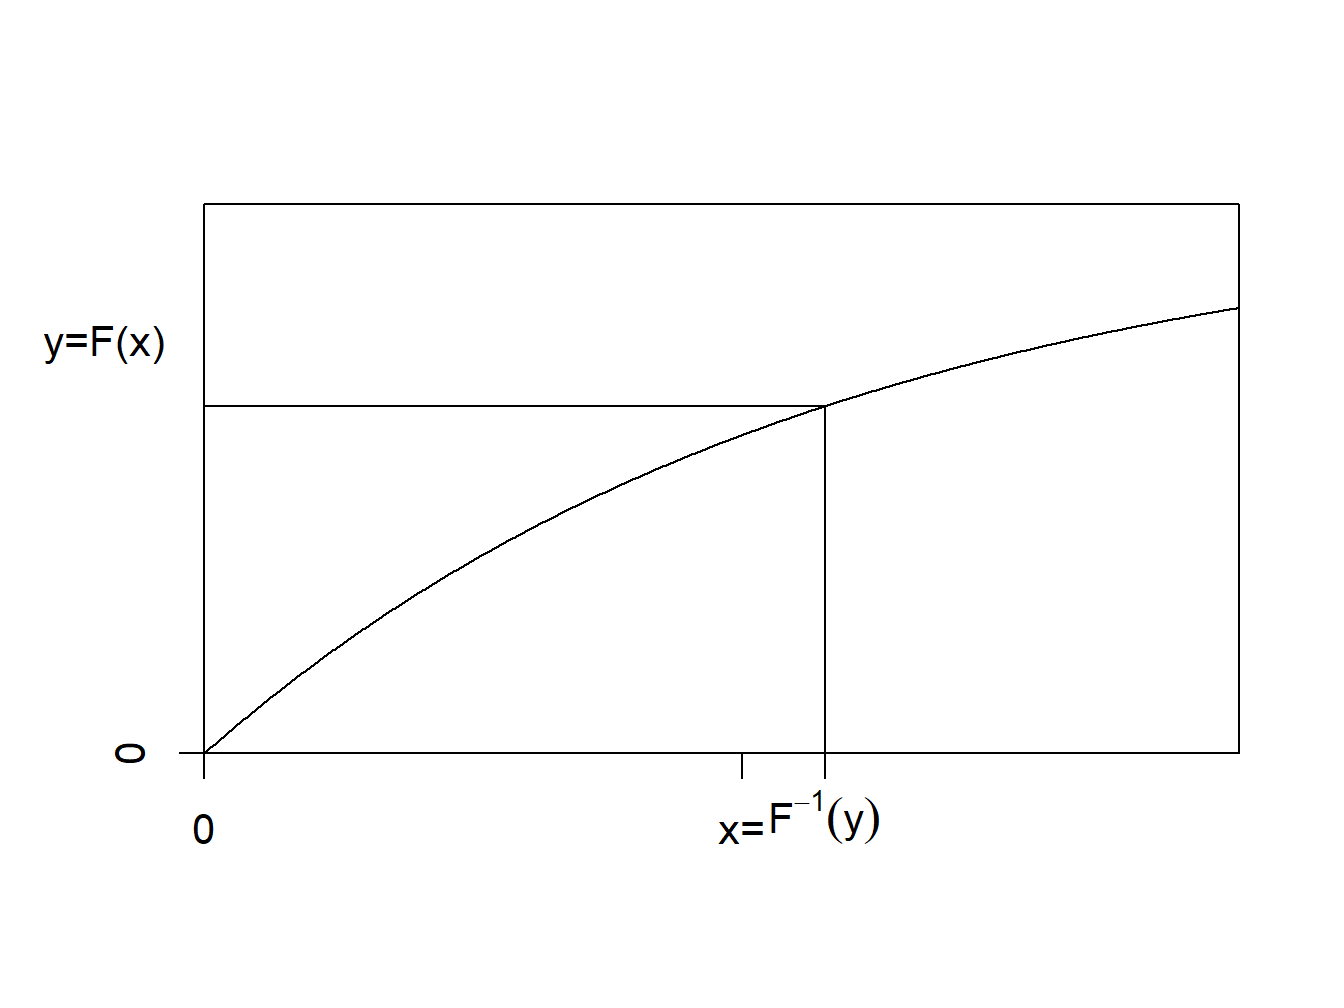
\includegraphics[width=0.6\linewidth]{LossDataAnalytics_files/figure-latex/InverseDF-1} 

}

\caption{Inverse of a Distribution Function}\label{fig:InverseDF}
\end{figure}

The inverse transform result is available when the underlying random
variable is continuous, discrete or a mixture. Here is a series of
examples to illustrate its scope of applications.

\textbf{Exponential Distribution Example.} Suppose that we would like to
generate observations from an exponential distribution with scale
parameter \(\theta\) so that \(F(x) = 1 - e^{-x/\theta}\). To compute
the inverse transform, we can use the following steps: \[\begin{aligned}
 y = F(x) &\Leftrightarrow  y = 1-e^{-x/\theta} \\
  &\Leftrightarrow -\theta \ln(1-y) = x = F^{-1}(y) .\end{aligned}\]
Thus, if \(U\) has a uniform (0,1) distribution, then
\(X = -\theta \ln(1-U)\) has an exponential distribution with parameter
\(\theta\).

\emph{Some Numbers.} Take \(\theta = 10\) and generate three random
numbers to get

\begin{longtable}[]{@{}lrrr@{}}
\toprule
\(U\) & 0.26321364 & 0.196884752 & 0.897884218\tabularnewline
\(X = -10\ln(1-U)\) & 1.32658423 & 0.952221285 &
9.909071325\tabularnewline
\bottomrule
\end{longtable}

\textbf{Pareto Distribution Example.} Suppose that we would like to
generate observations from a Pareto distribution with parameters
\(\alpha\) and \(\theta\) so that
\(F(x) = 1 - \left(\frac{\theta}{x+\theta} \right)^{\alpha}\). To
compute the inverse transform, we can use the following steps:
\[\begin{aligned}
 y = F(x) &\Leftrightarrow 1-y = \left(\frac{\theta}{x+\theta} \right)^{\alpha} \\
  &\Leftrightarrow \left(1-y\right)^{-1/\alpha} = \frac{x+\theta}{\theta} = \frac{x}{\theta} +1 \\
    &\Leftrightarrow \theta \left((1-y)^{-1/\alpha} - 1\right) = x = F^{-1}(y) .\end{aligned}\]
Thus, \(X = \theta \left((1-U)^{-1/\alpha} - 1\right)\) has a Pareto
distribution with parameters \(\alpha\) and \(\theta\).

\textbf{Inverse Transform Justification.} Why does the random variable
\(X = F^{-1}(U)\) have a distribution function ``\(F\)''?

This is easy to establish in the continuous case. Because \(U\) is a
Uniform random variable on (0,1), we know that \(\Pr(U \le y) = y\), for
\(0 \le y \le 1\). Thus, \[\begin{aligned}
\Pr(X \le x) &= \Pr(F^{-1}(U) \le x) \\
 &= \Pr(F(F^{-1}(U)) \le F(x)) \\
&= \Pr(U \le F(x)) = F(x)\end{aligned}\] as required. The key step is
that \$ F(F\^{}\{-1\}(u)) = u\$ for each \(u\), which is clearly true
when \(F\) is strictly increasing.

\textbf{Bernoulli Distribution Example.} Suppose that we wish to
simulate random variables from a Bernoulli distribution with parameter
\(p=0.85\). A graph of the cumulative distribution function shows that
the quantile function can be written as

\begin{figure}

{\centering 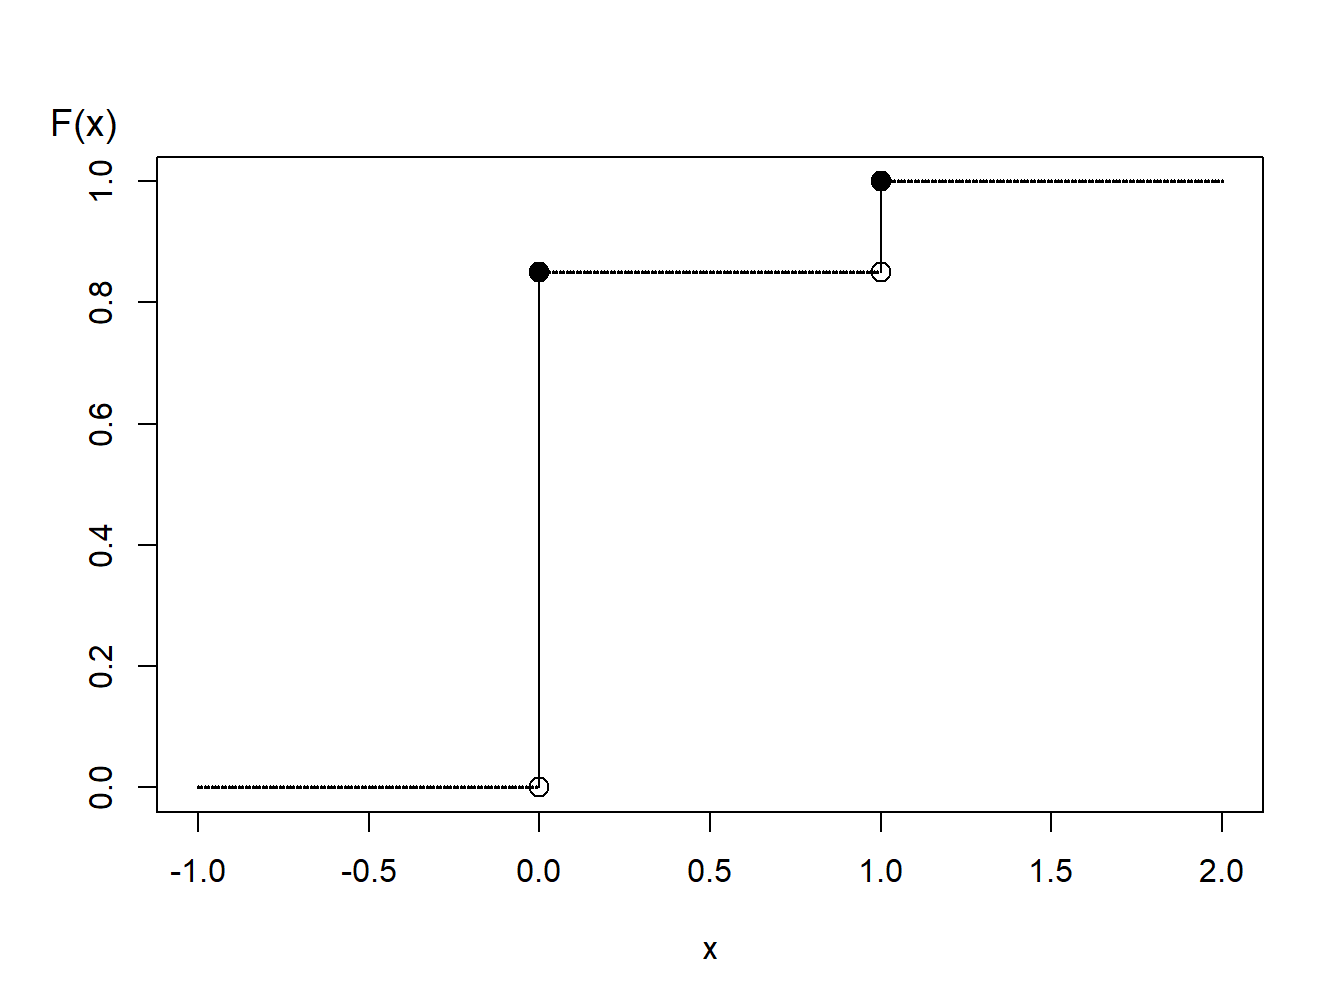
\includegraphics[width=0.5\linewidth]{LossDataAnalytics_files/figure-latex/BinaryDF-1} 

}

\caption{Distribution Function of a Binary Random Variable}\label{fig:BinaryDF}
\end{figure}

\[\begin{aligned}
F^{-1}(y) = \left\{ \begin{array}{cc}
              0 & 0<y \leq 0.85 \\
              1 & 0.85 < y  \leq  1.0 .
            \end{array} \right.\end{aligned}\]

Thus, with the inverse transform we may define \[\begin{aligned}
X = \left\{ \begin{array}{cc}
              0 & 0<U \leq 0.85  \\
              1 &  0.85 < U  \leq  1.0
            \end{array} \right.\end{aligned}\] \emph{Some Numbers.}
Generate three random numbers to get

\begin{longtable}[]{@{}lrrr@{}}
\toprule
\(U\) & 0.26321364 & 0.196884752 & 0.897884218\tabularnewline
\(X =F^{-1}(U)\) & 0 & 0 & 1\tabularnewline
\bottomrule
\end{longtable}

\textbf{Discrete Distribution Example.} Consider the time of a machine
failure in the first five years. The distribution of failure times is
given as:

\begin{longtable}[]{@{}lrrrrr@{}}
\toprule
Time (\(x\)) & 1 & 2 & 3 & 4 & 5\tabularnewline
probability & 0.1 & 0.2 & 0.1 & 0.4 & 0.2\tabularnewline
\(F(x)\) & 0.1 & 0.3 & 0.4 & 0.8 & 1.0\tabularnewline
\bottomrule
\end{longtable}

\begin{figure}

{\centering 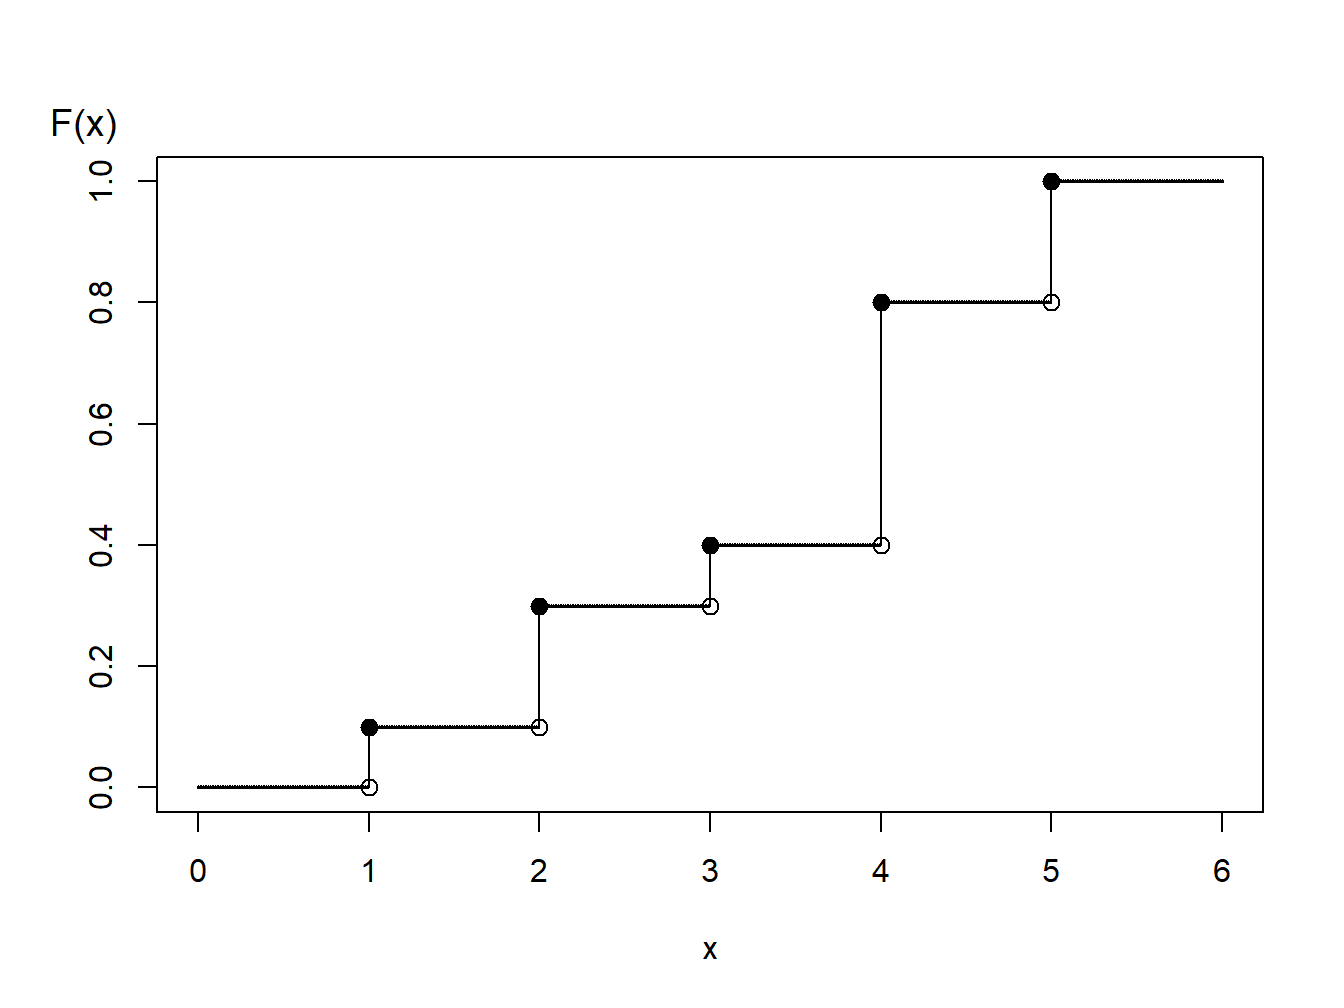
\includegraphics[width=0.8\linewidth]{LossDataAnalytics_files/figure-latex/DiscreteDF-1} 

}

\caption{Distribution Function of a Discrete Random Variable}\label{fig:DiscreteDF}
\end{figure}

Using the graph of the distribution function, with the inverse transform
we may define \[\begin{aligned}
X = \left\{ \begin{array}{cc}
              1 &   0<U  \leq 0.1  \\
              2 &  0.1 < U  \leq  0.3\\
              3 &  0.3 < U  \leq  0.4\\
              4 &  0.4 < U  \leq  0.8  \\
              5 &  0.8 < U  \leq  1.0     .
            \end{array} \right.\end{aligned}\]

For general discrete random variables there may not be an ordering of
outcomes. For example, a person could own one of five types of life
insurance products and we might use the following algorithm to generate
random outcomes:

\[\begin{aligned}
X = \left\{ \begin{array}{cc}
  \textrm{whole life} &   0<U  \leq 0.1  \\
 \textrm{endowment} &  0.1 < U  \leq  0.3\\
\textrm{term life} &  0.3 < U  \leq  0.4\\
  \textrm{universal life} &  0.4 < U  \leq  0.8  \\
  \textrm{variable life} &  0.8 < U  \leq  1.0 .
            \end{array} \right.\end{aligned}\]

Another analyst may use an alternative procedure such as:

\[\begin{aligned}
X = \left\{ \begin{array}{cc}
  \textrm{whole life} &   0.9<U<1.0  \\
 \textrm{endowment} &  0.7 \leq U < 0.9\\
\textrm{term life} &  0.6 \leq U < 0.7\\
  \textrm{universal life} &  0.2 \leq U < 0.6  \\
  \textrm{variable life} &  0 \leq U < 0.2 .
            \end{array} \right.\end{aligned}\]

Both algorithms produce (in the long-run) the same probabilities, e.g.,
\(\Pr(\textrm{whole life})=0.1\), and so forth. So, neither is
incorrect. You should be aware that there is ``more than one way to skin
a cat.'' (What an old expression!) Similarly, you could use an
alterative algorithm for ordered outcomes (such as failure times 1, 2,
3, 4, or 5, above).

\textbf{Mixed Distribution Example.} Consider a random variable that is
0 with probability 70\% and is exponentially distributed with parameter
\(\theta= 10,000\) with probability 30\%. In practice, this might
correspond to a 70\% chance of having no insurance claims and a 30\%
chance of a claim - if a claim occurs, then it is exponentially
distributed. The distribution function is given as

\[\begin{aligned}
F(y) = \left\{ \begin{array}{cc}
              0 &  x<0  \\
              1 - 0.3 \exp(-x/10000) & x \ge 0 .
            \end{array} \right.\end{aligned}\]

\begin{figure}

{\centering 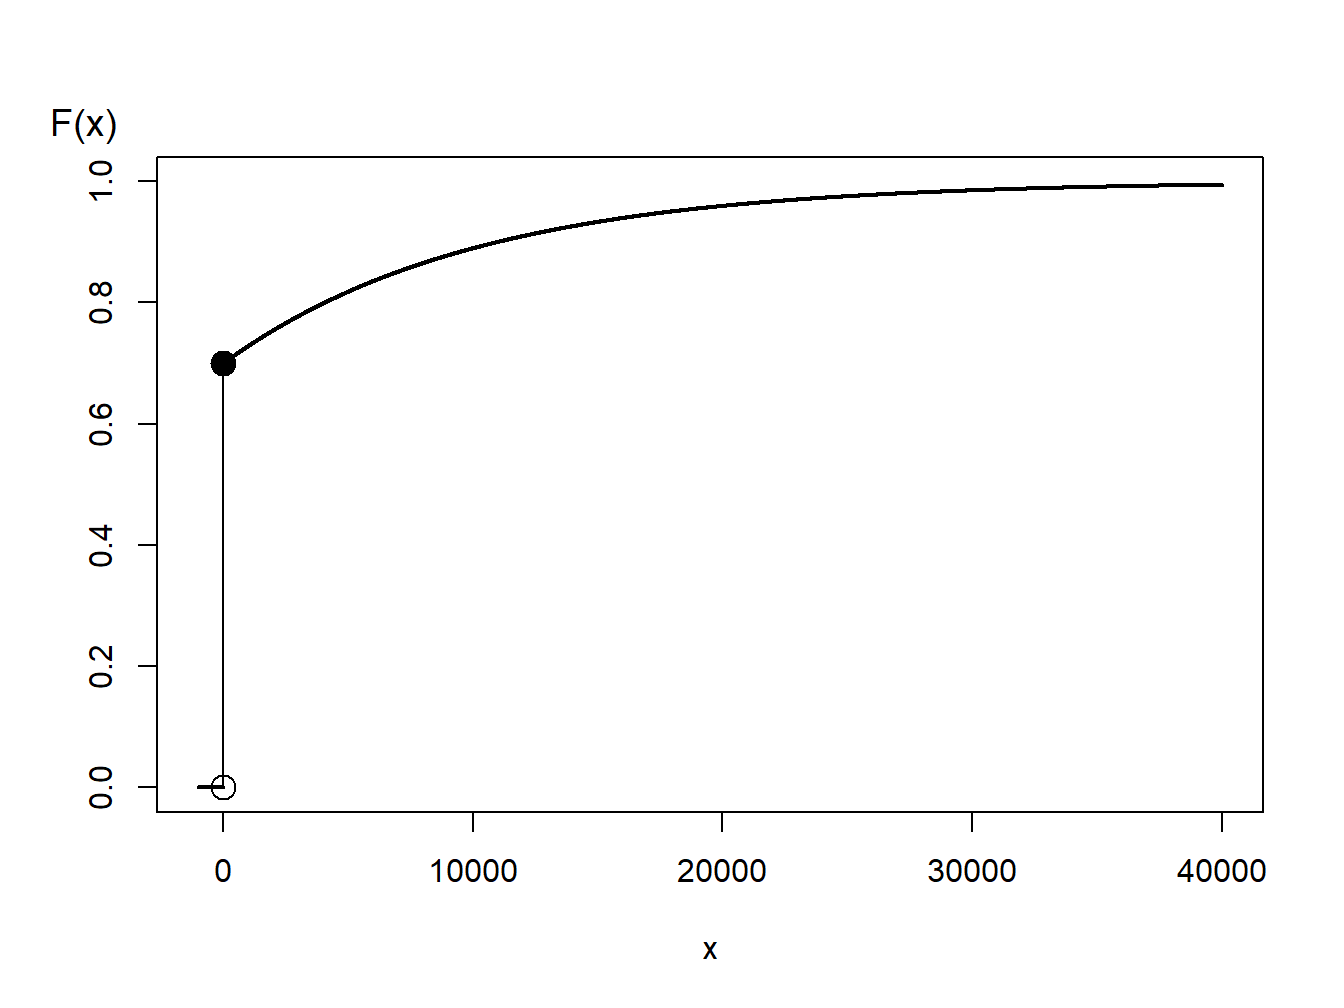
\includegraphics[width=0.6\linewidth]{LossDataAnalytics_files/figure-latex/MixedDF-1} 

}

\caption{Distribution Function of a Hybrid Random Variable}\label{fig:MixedDF}
\end{figure}

From the graph, we can see that the inverse transform for generating
random variables with this distribution function is

\[\begin{aligned}
X = F^{-1}(U) = \left\{ \begin{array}{cc}
              0 &  0< U  \leq  0.7  \\
              -1000 \ln (\frac{1-U}{0.3}) & 0.7 < U < 1 .
            \end{array} \right.\end{aligned}\]

As you have seen, for the discrete and mixed random variables, the key
is to draw a graph of the distribution function that allows you to
visualize potential values of the inverse function.

\section{How Many Simulated Values?}\label{how-many-simulated-values}

There are many topics to be described in the study of simulation (and
fortunately many good sources to help you). The best way to appreciate
simulation is to experience it. One topic that inevitably comes up is
the number of simulated trials needed to rid yourself of sampling
variability so that you may focus on patterns of interest.

How many simulated values are recommended? 100? 1,000,000? We can use
the central limit theorem to respond to this question. Suppose that we
wish to use simulation to calculate \(\mathrm{E~}h(X)\), where
\(h(\cdot)\) is some known function. Then, based on \(R\) simulations
(replications), we get \$ X\_1,\ldots,X\_R\$. From this simulated
sample, we calculate a sample average
\[\overline{h}_R=\frac{1}{R}\sum_{i=1}^{R} h(X_i)\] and a sample
standard deviation
\[s_{h,R}^2 = \frac{1}{R} \sum_{i=1}^{R}\left( h(X_i) -\overline{h}_R
\right) ^2.\] So, \(\overline{h}_R\) is your best estimate of
\(\mathrm{E~}h(X)\) and \(s_{h,R}^2\) provides an indication of the
uncertainty of your estimate. As one criterion for your confidence in
the result, suppose that you wish to be within 1\% of the mean with 95\%
certainty. According to the central limit theorem, your estimate should
be approximately normally distributed. Thus, you should continue your
simulation until \[\frac{.01\overline{h}_R}{s_{h,R}/\sqrt{R}}\geq 1.96\]
or equivalently \[R \geq 38,416\frac{s_{h,R}^2}{\overline{h}_R^2}.\]
This criterion is a direct application of the approximate normality
(recall that 1.96 is the 97.5th percentile of the standard normal
curve). Note that \(\overline{h}_R\) and \(s_{h,R}\) are not known in
advance, so you will have to come up with estimates as you go
(sequentially), either by doing a little pilot study in advance or by
interrupting your procedure intermittently to see if the criterion is
satisfied.

\chapter{Portfolio Management including
Reinsurance}\label{portfolio-management-including-reinsurance}

\subsection{Overview:}\label{overview}

Define \(S\) to be (random) obligations that arise from a collection
(portfolio) of insurance contracts

\begin{itemize}
\item
  We are particularly interested in probabilities of large outcomes and
  so formalize the notion of a heavy-tail distribution
\item
  How much in assets does an insurer need to retain to meet obligations
  arising from the random \(S\)? A study of risk measures helps to
  address this question
\item
  As with policyholders, insurers also seek mechanisms in order to
  spread risks. A company that sells insurance to an insurance company
  is known as a reinsurer
\end{itemize}

\section{Tails of Distributions}\label{tails-of-distributions}

\begin{itemize}
\item
  The \textbf{tail} of a distribution (more specifically: the
  \textbf{right tail}) is the portion of the distribution corresponding
  to large values of the r.v.
\item
  Understanding large possible loss values is important because they
  have the greatest impact on the total of losses.
\item
  R.v.'s that tend to assign higher probabilities to larger values are
  said to be \textbf{heavier tailed}.
\item
  When choosing models, tail weight can help narrow choices or can
  confirm a choice for a model.
\end{itemize}

\subsubsection{Classification Based on
Moments}\label{classification-based-on-moments}

\begin{itemize}
\item
  One way of classifying distributions:
\item
  are all moments finite, or not?
\item
  The \textbf{finiteness} of \textbf{all positive moments} indicates a
  (relatively) light right tail.
\item
  The \textbf{finiteness} of only positive moments \textbf{up to a
  certain value} indicates a heavy right tail.
\item
  \textbf{KPW Example 3.9}: demonstrate that for the gamma distribution
  all positive moments are finite but for the Pareto distribution they
  are not.
\item
  For the gamma distribution \[\begin{aligned}
  \mu_k^{'} &= \int_0^{\infty} x^k \frac{x^{\alpha-1} e^{-x/\theta}}{\Gamma(\alpha) \theta^{\alpha}} dx \\
  &= \int_0^{\infty} (y\theta)^k  \frac{(y\theta)^{\alpha-1} e^{-y}}{\Gamma(\alpha) \theta^{\alpha}} \theta dy \\
  &= \frac{\theta^k}{\Gamma(\alpha)} \Gamma(\alpha+k) < \infty \ \ \ \text{for\ all}\ k>0.\end{aligned}\]
\item
  \textbf{KPW Example 3.9}: demonstrate that for the gamma distribution
  all positive moments exist but for the Pareto distribution they do
  not.
\item
  For the Pareto distribution \[\begin{aligned}
  \mu_k^{'} &= \int_0^{\infty} x^k \frac{\alpha \theta^{\alpha}}{(x+\theta)^{\alpha+1}} dx \\
  &= \int_{\theta}^{\infty} (y-\theta)^k \frac{\alpha \theta^{\alpha}}{y^{\alpha+1}} dy \\
  &= \alpha \cdot \theta^{\alpha} \int_{\theta}^{\infty} \sum_{j=0}^k \left(\begin{array}{c}
   k \\
   j
   \end{array} \right) y^{j-\alpha-1} (-\theta)^{k-j} dy,\end{aligned}\]
  for integer values of \(k\).
\item
  This integral is finite only if
  \(\int_{\theta}^{\infty} y^{j-\alpha-1} dy = \frac{y^{j-\alpha}}{j-\alpha}\big{|}_{\theta}^{\infty}\)
  is finite.
\item
  Finiteness occurs when \(j-\alpha < 0\) for \(j=1, \ldots,k\). Or,
  equivalently, \(k< \alpha\).
\item
  Pareto is said to have a heavy tail, and gamma has a light tail.
\end{itemize}

\subsubsection{Comparison Based on Limiting Tail
Behavior}\label{comparison-based-on-limiting-tail-behavior}

\begin{itemize}
\item
  Consider two distributions with the same mean.
\item
  If ratio of \(S_1(.)\) and \(S_2(.)\) diverges to infinity, then
  distribution 1 has a heavier tail than distribution 2.
\item
  Thus, we examine \[\begin{aligned}
  \lim_{x\to \infty} \frac{S_1(x)}{S_2(x)} &= \lim_{x \to \infty} \frac{S_1^{'}(x)}{S_2^{'}(x)} \\
  &= \lim_{x \to \infty} \frac{-f_1(x)}{-f_2(x)} = \lim_{x\to \infty} \frac{f_1(x)}{f_2(x)}.\end{aligned}\]
\item
  \textbf{KPW Example 3.10}: demonstrate that Pareto distribution has a
  heavier tail than the gamma distribution using the limit of the ratio
  of their density functions.
\item
  We consider \[\begin{aligned}
  \lim_{x\to \infty} \frac{f_{\text{Pareto}}(x)}{f_{\text{gamma}}(x)} &= \lim_{x \to \infty} \frac{\alpha \theta^{\alpha} (x+ \theta)^{-\alpha-1}}{x^{\tau-1} e^{-x/\lambda} \lambda^{-\tau} \Gamma(\tau)^{-1}} \\
  &= c \lim_{x\to \infty} \frac{e^{x/\lambda}}{(x+\theta)^{\alpha+1} x^{\tau-1}} \\
  &= \infty\end{aligned}\]
\item
  Exponentials go to infinity faster than polynomials, thus the limit is
  infinity.
\end{itemize}

\section{Measures of Risk}\label{measures-of-risk}

\begin{itemize}
\item
  A \textbf{risk measure} is a mapping from the r.v. representing the
  loss associated with the risks to the real line.
\item
  A risk measure gives a single number that is intended to quantify the
  risk.

  \begin{itemize}
  \tightlist
  \item
    For example, the standard deviation is a risk measure.
  \end{itemize}
\item
  Notation: \(\rho(X)\).
\item
  We briefly mention:

  \begin{itemize}
  \item
    \textbf{VaR}: Value at Risk;
  \item
    \textbf{TVaR}: Tail Value at Risk.
  \end{itemize}
\end{itemize}

\subsubsection{Value at Risk}\label{value-at-risk}

\begin{itemize}
\item
  Say \(F_X(x)\) represents the cdf of outcomes over a fixed period of
  time, e.g.~one year, of a portfolio of risks.
\item
  We consider positive values of \(X\) as losses.
\item
  \textbf{Definition 3.11}: let \(X\) denote a loss r.v., then the
  \textbf{Value-at-Risk} of \(X\) at the \(100p\%\) level, denoted
  \(VaR_p(X)\) or \(\pi_p\), is the \(100p\) percentile (or quantile) of
  the distribution of \(X\).
\item
  E.g. for continuous distributions we have \[\begin{aligned}
  P(X> \pi_p) &= 1-p.\end{aligned}\]
\item
  VaR has become the standard risk measure used to evaluate exposure to
  risk.
\item
  \textbf{VaR} is the \textbf{amount of capital} required to ensure,
  with a \textbf{high degree of certainty}, that the \textbf{enterprise
  does not become technically insolvent}.
\item
  Which degree of certainty?

  \begin{itemize}
  \item
    95\(\%\)?
  \item
    in Solvency II \(99.5\%\) (or: ruin probability of 1 in 200).
  \end{itemize}
\item
  \textbf{VaR is not subadditive}.

  \begin{itemize}
  \item
    Subadditivity of a risk measure \(\rho(.)\) requires
    \[\begin{aligned}
    \rho(X+Y) \leq \rho(X)+\rho(Y).\end{aligned}\]
  \item
    Intuition behind subadditivity: combining risks is less riskier than
    holding them separately.
  \end{itemize}
\item
  \textbf{Example:} let \(X\) and \(Y\) be i.i.d. r.v.'s which are
  \(\text{Bern}(0.02)\) distributed.

  \begin{itemize}
  \item
    Then, \(P(X\leq 0) = 0.98\) and \(P(Y\leq 0)=0.98\). Thus,
    \(F_X^{-1}(0.975)=F_Y^{-1}(0.975)=0\).
  \item
    For the sum, \(X+Y\), we have \(P[X+Y=0]=0.98 \cdot 0.98=0.9604\).
    Thus, \(F_{X+Y}^{-1}(0.975)>0\).
  \item
    VaR is not subadditive, since \(\text{VaR}(X+Y)\) in this case is
    larger than \(\text{VaR}(X)+\text{VaR}(Y)\).
  \end{itemize}
\item
  Another \textbf{drawback of VaR}:

  \begin{itemize}
  \item
    it is a single quantile risk measure of a predetermined level \(p\);
  \item
    no information about the thickness of the upper tail of the
    distribution function from \(\text{VaR}_p\) on;
  \item
    whereas stakeholders are interested in both frequency and severity
    of default.
  \end{itemize}
\item
  Therefore: study other risk measures, e.g. \textbf{Tail Value at Risk}
  (TVaR).
\end{itemize}

\subsubsection{Tail Value at Risk}\label{tail-value-at-risk}

\begin{itemize}
\item
  \textbf{Definition 3.12:} let \(X\) denote a loss r.v., then the Tail
  Value at Risk of \(X\) at the \(100p\%\) security level,
  \(\text{TVaR}(p)\), is the \textbf{expected loss} \textbf{given that
  the loss exceeds the \(100p\) percentile} (or: quantile) of the
  distribution of \(X\).
\item
  We have (assume continuous distribution) \[\begin{aligned}
  \text{TVaR}_p(X) &= E(X|X>\pi_p) \\
  &= \frac{\int_{\pi_p}^{\infty} x\cdot f(x) dx}{1-F(\pi_p)}.\end{aligned}\]
\item
  We can rewrite this as \textbf{the usual definition of TVaR}
  \[\begin{aligned}
  \text{TVaR}_p(X) &= \frac{\int_{\pi_p}^{\infty} x dF_X(x)}{1-p} \\
  &= \frac{\int_p^1 \text{VaR}_u(X) du}{1-p},\end{aligned}\] using the
  substitution \(F_X(x) = u\) and thus \(x=F_X^{-1}(u)\).
\item
  From the definition \[\begin{aligned}
  \text{TVaR}_p(X) &= \frac{\int_p^1 \text{VaR}_u(X) du}{1-p},\end{aligned}\]
  we understand

  \begin{itemize}
  \item
    TVaR is the \textbf{arithmetic average} of the quantiles of \(X\),
    from level \(p\) on;
  \item
    TVaR is averaging high level VaR;
  \item
    TVaR \textbf{tells us much more about the tail} of the distribution
    than does VaR alone.
  \end{itemize}
\item
  Finally, TVaR can also be written as \[\begin{aligned}
  \text{TVaR}_p(X) &= E(X|X>\pi_p) \\
  &= \frac{\int_{\pi_p}^{\infty} x f(x)dx}{1-p} \\
  &= \pi_p + \frac{\int_{\pi_p}^{\infty} (x-\pi_p) f(x) dx}{1-p} \\
  &= \text{VaR}_p(X) + e(\pi_p),\end{aligned}\] with \(e(\pi_p)\) the
  mean excess loss function evaluated at the \(100p\)th percentile.
\item
  We can understand these connections as follows. (Assume continuous
  r.v.'s)
\item
  The relation \[\begin{aligned}
  \text{CTE}_p(X) &= \text{TVaR}_{F_X(\pi_p)}(X),\end{aligned}\] then
  follows immediately by combining the other two expressions.
\item
  TVaR is a coherent risk measure, see e.g.
  \href{http://onderwijsaanbod.kuleuven.be/syllabi/e/D0R57BE.htm\#activetab=doelstellingen_idp1406608}{Foundations
  of Risk Measurement} course.
\item
  Thus, \(\text{TVaR}(X+Y) \leq \text{TVaR}(X)+\text{TVaR}(Y)\).
\item
  When using this risk measure, we never encounter a situation where
  combining risks is viewed as being riskier than keeping them separate.
\item
  \textbf{KPW Example 3.18} \emph{(Tail comparisons)} Consider three
  loss distributions for an insurance company. Losses for the next year
  are estimated to be on average 100 million with standard deviation
  223.607 million. You are interested in finding high quantiles of the
  distribution of losses. Using the normal, Pareto, and Weibull
  distributions, obtain the VaR at the 90\%, 99\%, and 99.99\% security
  levels.
\item
  \textbf{Solution}
\item
  Normal distribution has a lighter tail than the others, and thus
  smaller quantiles.
\item
  Pareto and Weibull with \(\tau<1\) have heavy tails, and thus
  relatively larger extreme quantiles.
\item
  \textbf{Example 3.18} \emph{(Tail comparisons)} Consider three loss
  distributions for an insurance company. Losses for the next year are
  estimated to be on average 100 million with standard deviation 223.607
  million. You are interested in finding high quantiles of the
  distribution of losses. Using the normal, Pareto, and Weibull
  distributions, obtain the VaR at the 99\%, 99.9\%, and 99.99\%
  security levels.

\begin{verbatim}
> qnorm(c(0.9,0.99,0.999),mu,sigma)
[1] 386.5639 620.1877 790.9976
> qpareto(c(0.9,0.99,0.999),alpha,s)
[1]  226.7830  796.4362 2227.3411
> qweibull(c(0.9,0.99,0.999),tau,theta)
[1]  265.0949 1060.3796 2385.8541
\end{verbatim}
\item
  We learn from Example 3.18 that results vary widely depending on the
  choice of distribution.
\item
  Thus, the selection of an \textbf{appropriate loss model} is highly
  important.
\item
  To obtain numerical values of VaR or TVaR:

  \begin{itemize}
  \item
    estimate from the data directly;
  \item
    or use distributional formulas, and plug in parameter estimates.
  \end{itemize}
\item
  When estimating VaR directly from the data:

  \begin{itemize}
  \item
    use R to get quantile from the empirical distribution;
  \item
    R has 9 ways to estimate a VaR at level \(p\) from a sample of size
    \(n\), differing in the way the interpolation between order
    statistics close to \(np\) .
  \end{itemize}
\item
  When estimating TVaR directly from the data:

  \begin{itemize}
  \tightlist
  \item
    take average of all observations that exceed the threshold
    (i.e.\(\pi_p\));
  \end{itemize}
\item
  \textbf{Caution:} we need a large number of observations (and a large
  number of observations \(> \pi_p\)) in order to get reliable
  estimates.
\item
  When not may observations in excess of the threshold are available:

  \begin{itemize}
  \item
    construct a loss model;
  \item
    calculate values of VaR and TVaR directly from the fitted
    distribution.
  \end{itemize}
\item
  For example \[\begin{aligned}
    \text{TVaR}_p(X) &= E(X|X>\pi_p) \\
  &= \pi_p + \frac{\int_{\pi_p}^{\infty} (x-\pi_p) f(x) dx}{1-p} \\
  &= \pi_p + \frac{\int_{-\infty}^{\infty} (x-\pi_p) f(x) dx -\int_{-\infty}^{\pi_p} (x-\pi_p) f(x) dx }{1-p} \\
  &= \pi_p + \frac{E(X)-\int_{-\infty}^{\pi_p} xf(x) dx -\pi_p (1-F(\pi_p))}{1-p} \\
  &= \pi_p + \frac{E(X) - E[\min{(X,\pi_p)}]}{1-p} = \pi_p + \frac{E(X)-E(X \wedge \pi_p)}{1-p},\end{aligned}\]
  see Appendix A for those expressions.
\end{itemize}

\section{Reinsurance}\label{reinsurance-1}

\begin{itemize}
\item
  A major difference between reinsurance and primary insurance is that a
  reinsurance program is generally tailored more closely to the buyer
\item
  There are two major types of reinsurance

  \begin{itemize}
  \item
    Proportional
  \item
    Excess of Loss
  \end{itemize}
\item
  A proportional treaty is an agreement between a reinsurer and a ceding
  company (the reinsured) in which the reinsurer assumes a given percent
  of losses and premium.
\end{itemize}

\subsection{Proportional Reinsurance}\label{proportional-reinsurance}

\begin{itemize}
\item
  A proportional treaty is an agreement between a reinsurer and a ceding
  company (the reinsured) in which the reinsurer assumes a given percent
  of losses and premium.
\item
  The simplest example of a proportional treaty is called \emph{Quota
  Share}.

  \begin{itemize}
  \item
    In a quota share treaty, the reinsurer receives a flat percent, say
    50\%, of the premium for the book of business reinsured.
  \item
    In exchange, the reinsurer pays 50\% of losses, including allocated
    loss adjustment expenses
  \item
    The reinsurer also pays the ceding company a ceding commission which
    is designed to reflect the differences in underwriting expenses
    incurred.
  \end{itemize}
\item
  The amounts paid by the direct insurer and the reinsurer are defined
  as follows:
\end{itemize}

\begin{equation*}
Y_{insurer} =
\begin{cases}
X & X \le M\\
M & X >M \\
\end{cases} \ \ \ \ = \min(X,M) = X \wedge M
\end{equation*}

\begin{equation*}
Y_{reinsurer} =
\begin{cases}
0 & X \le M\\
X- M & X >M \\
\end{cases} \ \ \ \  = \max(0,X-M)
\end{equation*}

Note that \(Y_{insurer}+Y_{reinsurer}=X\).

\subsection{Surplus Share Proportional
Treaty}\label{surplus-share-proportional-treaty}

\begin{itemize}
\item
  Another proportional treaty is known as \emph{Surplus Share}; these
  are common in property business.
\item
  A surplus share treaty allows the reinsured to limit its exposure on
  any one risk to a given amount (the \emph{retained line}).
\item
  The reinsurer assumes a part of the risk in proportion to the amount
  that the insured value exceeds the retained line, up to a given limit
  (expressed as a multiple of the retained line, or number of lines).
\item
  For example, let the retained Line be \$100,000 and let the given
  limit be 4 lines (\$400,000). Then, if \(X\) is the loss, the
  reinsurer's portion is \(\min(400000, (X-100000)_+)\).
\end{itemize}

\subsection{Excess of Loss
Reinsurance}\label{excess-of-loss-reinsurance}

\begin{itemize}
\item
  Under this arrangement, the direct insurer sets a retention level
  \(M (>0)\) and pays in full any claim for which \(X \le M\).
\item
  The direct insurer retains an amount \(M\) of the risk.
\item
  For claims for which \(X > M\), the direct insurer pays \(M\) and the
  reinsurer pays the remaining amount \(X-M\).
\item
  The amounts paid by the direct insurer and the reinsurer are defined
  as follows.
\end{itemize}

\begin{equation*}
Y_{insurer} = c X \ \ \ \ \ Y_{reinsurer} = (1-c) X
\end{equation*}

Note that \(Y_{insurer}+Y_{reinsurer}=X\).

\subsection{Relations with Personal
Insurance}\label{relations-with-personal-insurance}

\begin{itemize}
\item
  We have already seen the needed tools to handle reinsurance in the
  context of personal insurance

  \begin{itemize}
  \item
    For a proportional reinsurance, the transformation \$Y\_\{insurer\}
    = c X \$ is the same as a coinsurance adjustment in personal
    insurance
  \item
    For excess of loss reinsurance, the transformation
    \(Y_{reinsurer} = \max(0,X-M)\) is the same as an insurer's payment
    with a deductible \(M\) and \(Y_{insurer} = \min(X,M) = X \wedge M\)
    is equivalent to what a policyholder pays with deductible \(M\).
  \end{itemize}
\item
  Reinsurance applications suggest introducing \emph{layers of
  coverage}, a (small) mathematical extension.
\end{itemize}

\subsection{Layers of Coverage}\label{layers-of-coverage}

\begin{itemize}
\item
  Instead of simply an insurer and reinsurer or an insurer and a
  policyholder, think about the situation with all three parties, a
  policyholder, insurer, and reinsurer, who agree on how to share a
  risk.
\item
  In general, we consider \(k\) parties. If \(k=4\), it could be an
  insurer and three different reinsurers.
\item
  Consider a simple example:

  \begin{itemize}
  \item
    Suppose that there are \(k=3\) parties. The first party is
    responsible for the first 100 of claims, the second responsible for
    claims from 100 to 3000, and the third responsible for claims above
    3000.
  \item
    If there are four claims in the amounts 50, 600, 1800 and 4000, they
    would be allocated to the parties as follows:
  \end{itemize}
\end{itemize}

\begin{longtable}[]{@{}lccccl@{}}
\toprule
Layer & Claim 1 & Claim 2 & Claim 3 & Claim 4 & Total\tabularnewline
\midrule
\endhead
(0, 100{]} & 50 & 100 & 100 & 100 & 350\tabularnewline
(100, 3000{]} & 0 & 500 & 1700 & 2900 & 5100\tabularnewline
(3000, \(\infty\)) & 0 & 0 & 0 & 1000 & 1000\tabularnewline
Total & 50 & 600 & 1800 & 4000 & 6450\tabularnewline
\bottomrule
\end{longtable}

\begin{itemize}
\item
  Mathematically, partition the positive real line into \(k\) intervals
  using the cut-points
  \(0 = c_0 < c_1 < \cdots < c_{k-1} < c_k = \infty\).

  \begin{itemize}
  \tightlist
  \item
    The \(j\)th interval is \((c_{j-1}, c_j]\).
  \end{itemize}
\item
  Let \(Y_j\) be the amount of risk shared by the \(j\)th party
\item
  To illustrate, if a loss \(x\) is such that \(c_{j-1} <x \le c_j\),
  then \[\left(\begin{array}{c}
  Y_1\\ Y_2 \\ \vdots \\ Y_j \\Y_{j+1} \\ \vdots \\Y_k
  \end{array}\right)
  =\left(\begin{array}{c}
  c_1-c_0 \\ c_2-c_1  \\ \vdots \\ x-c_{j-1}  \\ 0 \\ \vdots \\0
  \end{array}\right)\]
\item
  More succinctly, we can write \[Y_j = \min(X,c_j) - \min(X,c_{j-1})\]
\item
  With the expression \(Y_j = min(X,c_j) - min(X,c_{j-1})\), we see that
  the \(j\)th party is responsible for claims in the interval
  \((c_{j-1}, c_j]\)
\item
  Note that \(X = Y_1 + Y_2 + \cdots + Y_k\)
\item
  The parties need not be different.

  \begin{itemize}
  \item
    For example, suppose that a policyholder is responsible for the
    first 500 of claims and all claims in excess of 100,000. The insurer
    takes claims between 100 and 100,000.
  \item
    Then, we would use \(c_1 = 100\), \(c_2 =100000\).
  \item
    The policyholder is responsible for \(Y_1 =\min(X,100)\) and
    \(Y_3 = X - \min(X,100000) = \max(0, X-100000)\).
  \end{itemize}
\item
  See the Wisconsin Property Fund site for more info on layers of
  reinsurance,
  \url{https://sites.google.com/a/wisc.edu/local-government-property-insurance-fund/home/reinsurance}
\end{itemize}

\chapter{Technical Supplement: Statistical
Inference}\label{technical-supplement-statistical-inference}

\section{Overview of Statistical
Inference}\label{overview-of-statistical-inference}

\begin{itemize}
\item
  A set of data (a \textbf{sample}) has been collected that is
  considered representative of a larger set (the \textbf{population}).
  This relationship is known as the \textbf{sampling frame}.
\item
  Often, we can describe the distribution of the population in terms of
  a limited (finite) number of terms called \textbf{parameters}. These
  are referred to as \emph{parametric distributions}. With
  \textbf{nonparametric} analysis, we do not limit ourselves to only a
  few parameters.
\item
  The \textbf{statistical inference} goal is to say something about the
  (larger) population based on the observed sample (we ``\emph{infer},''
  not ``\emph{deduce}''). There are three types of statements:

  \begin{enumerate}
  \def\labelenumi{\arabic{enumi}.}
  \item
    \textbf{Estimation}
  \item
    \textbf{Hypothesis Testing}
  \item
    \textbf{Prediction}
  \end{enumerate}
\end{itemize}

\subsubsection{Wisconsin Property Fund}\label{wisconsin-property-fund}

\begin{itemize}
\item
  Discuss ideas of statistical inference in the context of a sample from
  the Wisconsin Property Fund
\item
  Specifically, consider 1,377 \emph{individual} claims from 2010
  experience (slightly different from the analysis of 403 average claims
  in Chapter 1)
\end{itemize}

\begin{longtable}[]{@{}llrllrlr@{}}
\toprule
\begin{minipage}[t]{0.12\columnwidth}\raggedright\strut
\strut
\end{minipage} & \begin{minipage}[t]{0.12\columnwidth}\raggedright\strut
\strut
\end{minipage} & \begin{minipage}[t]{0.12\columnwidth}\raggedleft\strut
First\strut
\end{minipage} & \begin{minipage}[t]{0.12\columnwidth}\raggedright\strut
\strut
\end{minipage} & \begin{minipage}[t]{0.12\columnwidth}\raggedright\strut
\strut
\end{minipage} & \begin{minipage}[t]{0.12\columnwidth}\raggedleft\strut
Third\strut
\end{minipage} & \begin{minipage}[t]{0.12\columnwidth}\raggedright\strut
\strut
\end{minipage} & \begin{minipage}[t]{0.12\columnwidth}\raggedleft\strut
Standard\strut
\end{minipage}\tabularnewline
\begin{minipage}[t]{0.12\columnwidth}\raggedright\strut
\strut
\end{minipage} & \begin{minipage}[t]{0.12\columnwidth}\raggedright\strut
Minimum\strut
\end{minipage} & \begin{minipage}[t]{0.12\columnwidth}\raggedleft\strut
Quartile\strut
\end{minipage} & \begin{minipage}[t]{0.12\columnwidth}\raggedright\strut
Median\strut
\end{minipage} & \begin{minipage}[t]{0.12\columnwidth}\raggedright\strut
Mean\strut
\end{minipage} & \begin{minipage}[t]{0.12\columnwidth}\raggedleft\strut
Quartile\strut
\end{minipage} & \begin{minipage}[t]{0.12\columnwidth}\raggedright\strut
Maximum\strut
\end{minipage} & \begin{minipage}[t]{0.12\columnwidth}\raggedleft\strut
Deviation\strut
\end{minipage}\tabularnewline
Claims & 1 & 788 & 2,250 & 26,620 & 6,171 & 12,920,000 &
368,030\tabularnewline
Logarithmic Claims & 0 & 6.670 & 7.719 & 7.804 & 8.728 & 16.370 &
1.683\tabularnewline
\bottomrule
\end{longtable}

\begin{Shaded}
\begin{Highlighting}[]
\NormalTok{ClaimLev <-}\StringTok{ }\KeywordTok{read.csv}\NormalTok{(}\StringTok{"Data/CLAIMLEVEL.csv"}\NormalTok{, }\DataTypeTok{header=}\OtherTok{TRUE}\NormalTok{)}
\NormalTok{ClaimLevBC10<-}\KeywordTok{subset}\NormalTok{(ClaimLev,Year==}\DecValTok{2010}\NormalTok{); }\KeywordTok{nrow}\NormalTok{(ClaimLevBC10)}
\end{Highlighting}
\end{Shaded}

\begin{verbatim}
## [1] 1377
\end{verbatim}

\begin{Shaded}
\begin{Highlighting}[]
\KeywordTok{par}\NormalTok{(}\DataTypeTok{mfrow=}\KeywordTok{c}\NormalTok{(}\DecValTok{1}\NormalTok{, }\DecValTok{2}\NormalTok{))}
\KeywordTok{hist}\NormalTok{(ClaimLevBC10$Claim, }\DataTypeTok{main=}\StringTok{""}\NormalTok{, }\DataTypeTok{xlab=}\StringTok{"Claims"}\NormalTok{)}
\KeywordTok{hist}\NormalTok{(}\KeywordTok{log}\NormalTok{(ClaimLevBC10$Claim), }\DataTypeTok{main=}\StringTok{""}\NormalTok{, }\DataTypeTok{xlab=}\StringTok{"Logarithmic Claims"}\NormalTok{)}
\end{Highlighting}
\end{Shaded}

\begin{figure}

{\centering 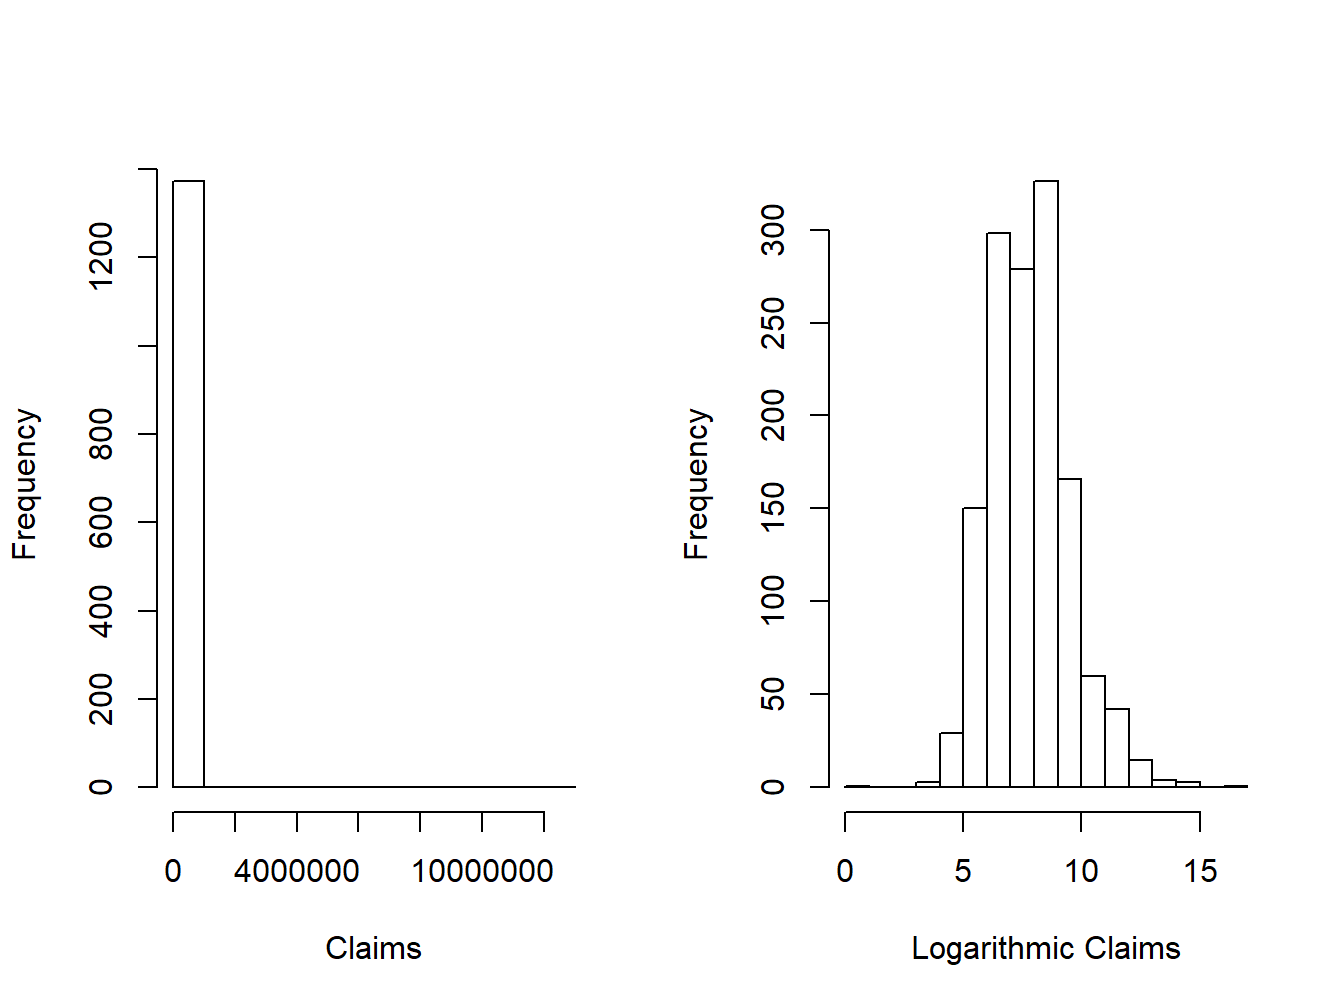
\includegraphics[width=0.8\linewidth]{LossDataAnalytics_files/figure-latex/ClaimDistn1-1} 

}

\caption{Distribution of Claims}\label{fig:ClaimDistn1}
\end{figure}

\subsubsection{Sampling Frame}\label{sampling-frame}

\begin{itemize}
\item
  In statistics, a sampling frame \textbf{error} occurs when the
  sampling frame, the list from which the sample is drawn, is not an
  adequate approximation of the population of interest.
\item
  For the property fund example, the sample consists of all 2010 claims

  \begin{itemize}
  \item
    The population might be all claims that could have potentially
    occurred in 2010.
  \item
    Or, it might be all claims that could potentially occur, such as in
    2010, 2011, and so forth
  \end{itemize}
\item
  A sample must be a representative subset of a population, or
  ``universe,'' of interest. If the sample is not representative, taking
  a larger sample does not eliminate bias; you simply repeat the same
  mistake over again and again.
\item
  A sample should be a representative subset of a population, or
  ``universe,'' of interest.
\item
  Formally

  \begin{itemize}
  \item
    We assume that the random variable \(X\) represents a draw from a
    population with distribution function F(.)
  \item
    We make several such draws (\(n\)), each unrelated to one another
    (statistically independent)
  \item
    Sometimes we say that \(X_1, \ldots, X_n\) is a random sample (with
    replacement) from F(.)
  \item
    Sometimes we say that \(X_1, \ldots, X_n\) are identically and
    independently distributed (\(iid\))
  \end{itemize}
\end{itemize}

\subsubsection{Describing the
Population}\label{describing-the-population}

\begin{itemize}
\item
  We think of the random variable \(X\) as a draw from the population
  with distribution function F(.)
\item
  There are several ways to summarize F(.). We might consider the mean,
  standard deviation, 95th percentile, and so on.

  \begin{itemize}
  \tightlist
  \item
    Because these summary stats do not depend on a specific parametric
    reference, they are \textbf{nonparametric} summary measures.
  \end{itemize}
\item
  In contrast, we can think of logarithmic claims as normally
  distributed with mean \(\mu\) and standard deviation \(\sigma\), that
  is, claims have a \emph{lognormal} distribution
\item
  We will also look at the gamma distribution, with parameters
  \(\alpha\) and \(\theta\), as a claims model

  \begin{itemize}
  \item
    The normal, lognormal, and gamma are examples of \textbf{parametric}
    distributions.
  \item
    The quantities \(\mu\), \(\sigma\), \(\alpha\), and \(\theta\) are
    known as \emph{parameters}. When we know the parameters of a
    distribution family, then we have knowledge of the entire
    distribution.
  \end{itemize}
\end{itemize}

\section{Estimation and Prediction}\label{estimation-and-prediction}

\subsubsection{Estimation}\label{estimation}

\begin{itemize}
\item
  Use \(\theta\) to denote a summary of the population.

  \begin{itemize}
  \item
    Parametric - It can be a parameter from a distribution such as
    \(\mu\) or \(\sigma\).
  \item
    Nonparametric - It can also be a nonparametric summary such as the
    mean or standard deviation.
  \end{itemize}
\item
  Let \(\hat{\theta} =\hat{\theta}(X_1, \ldots, X_n)\) be a function of
  the sample that provides proxy, or \textbf{estimate}, of \(\theta\).
  It is a function of the sample \(X_1, \ldots, X_n\).
\item
  In our property fund case,

  \begin{itemize}
  \item
    7.804 is a (nonparametric) estimate of the population expected
    logarithmic claim and 1.683 is an estimate of the corresponding
    standard deviation.
  \item
    These are (parametric) estimates of the normal distribution for
    logarithmic claims
  \item
    The estimate of the expected claim using the lognormal distribution
    is 10,106.8 (=\(\exp(7.804+1.683^2/2))\).
  \end{itemize}
\end{itemize}

\subsubsection{Lognormal Distribution and
Estimation}\label{lognormal-distribution-and-estimation}

\begin{itemize}
\item
  Assume that claims follow a lognormal distribution, so that
  logarithmic claims follow the familiar normal distribution.
\item
  Specifically, assume \(\ln X\) has a normal distribution with mean
  \(\mu\) and variance \(\sigma^2\), sometimes denoted as
  \(X \sim N(\mu, \sigma^2)\).
\item
  For the property data, estimates are \(\hat{\mu} =7.804\) and
  \(\hat{\sigma} = 1.683\). The ``hat'' notation is common. These are
  said to be \textbf{point estimates}, a single approximation of the
  corresponding parameter.
\item
  Under general maximum likelihood theory (that we will do in a little
  bit), these estimates typically have a normal distribution for large
  samples.

  \begin{itemize}
  \item
    Using notation, \(\hat{\theta}\) has an approximate normal
    distribution with mean \(\theta\) and variance, say,
    \(\mathrm{Var}(\hat{\theta})\).
  \item
    Take the square root of the variance and plug-in the estimate to
    define \(se(\hat{\theta}) = \sqrt{\mathrm{Var}(\hat{\theta})}\). A
    \textbf{standard error} is an estimated standard deviation.
  \item
    The next step in the mathematical statistics theory is to establish
    that \((\hat{\theta}-\theta)/se(\hat{\theta})\) has a
    \(t\)-distribution with ``degrees of freedom'' (a parameter of the
    distribution) equal to the sample size minus the dimension of
    \(\theta\).
  \end{itemize}
\item
  Assume that claims follow a lognormal distribution, so that
  logarithmic claims follow the familiar normal distribution.
\item
  Under general maximum likelihood theory

  \begin{itemize}
  \item
    \(\hat{\theta}\) has an approximate normal distribution with mean
    \(\theta\) and variance, say, \(\mathrm{Var}(\hat{\theta})\).
  \item
    Take the square root of the variance and plug-in the estimate to
    define \(se(\hat{\theta}) = \sqrt{\mathrm{Var}(\hat{\theta})}\). A
    \textbf{standard error} is an estimated standard deviation.
  \item
    \((\hat{\theta}-\theta)/se(\hat{\theta})\) has a \(t\)-distribution
    with ``degrees of freedom'' (a parameter of the distribution) equal
    to the sample size minus the dimension of \(\theta\).
  \item
    As an application, we can invert this result to get a
    \textbf{confidence interval} for \(\theta\).
  \end{itemize}
\item
  A pair of statistics, \(\hat{\theta}_1\) and \(\hat{\theta}_2\),
  provide an interval of the form \([\hat{\theta}_1, \hat{\theta}_2]\)
  This interval is a \(1-\alpha\) confidence interval for \(\theta\) if
  \(\Pr\left(\hat{\theta}_1 \le \theta \le \hat{\theta}_2\right) \ge 1-\alpha.\)
\item
  For example,
  \(\hat{\theta}_1 = \hat{\mu} - (t-value) \hat{\sigma}/\sqrt{n}\) and
  \(\hat{\theta}_2 = \hat{\mu} + (t-value) \hat{\sigma}/\sqrt{n}\)
  provide a confidence interval for \(\theta=\mu\). When
  \(\alpha = 0.05\), \(t-value \approx 1.96\).
\item
  For the property fund, (7.715235, 7.893208) is a 95\% confidence
  interval for \(\mu\).
\end{itemize}

\subsubsection{Lognormal Distribution and Hypothesis
Testing}\label{lognormal-distribution-and-hypothesis-testing}

An important statistical inference procedure involves verifying ideas
about parameters.

\begin{itemize}
\item
  To illustrate, in the property fund, assume that mean logarithmic
  claims have historically been approximately been
  \(\mu_0 = log(5000)= 8.517\). I might want to use 2010 data to see
  whether the mean of the distribution has changed. I also might want to
  test whether it has increased.
\item
  The actual 2010 average was \(\hat{\mu} =7.804\). Is this a
  significant departure from \(\mu_0 = 8.517\)?
\item
  One way to think about it is in terms of standard errors. The
  deviation is \((8.517-7.804)/(1.683/\sqrt{1377}) = 15.72\) standard
  errors. This is highly unlikely assuming an approximate normal
  distribution.
\item
  One hypothesis testing procedure begin with the calculation the test
  statistic \(t-stat=(\hat{\theta}-\theta_0)/se(\hat{\theta})\). Here,
  \(\theta_0\) is an assumed value of the parameter.
\item
  Then, one rejects the hypothesized value if the test statistic
  \(t-stat\) is ``unusual.'' To gauge ``unusual,'' use the same
  \(t\)-distribution as introduced for confidence intervals.
\item
  If you only want to know about a difference, this is known as a
  ``two-sided'' test; use the same \(t-value\) as the case for
  confidence intervals.
\item
  If you want to investigate whether there has been an increase (or
  decrease), then use a ``one-sided'' test.
\item
  Another useful concept in hypothesis testing is the \(p\)-value, which
  is short hand for probability value. For a data set, a \(p\)-value is
  defined to be the smallest significance level for which the null
  hypothesis would be rejected.
\end{itemize}

\subsubsection{Property Fund -- Other
Distributions}\label{property-fund-other-distributions}

\begin{itemize}
\item
  For numerical stability and extensions to regression applications,
  statistical packages often work with transformed version of parameters
\item
  The following estimates are from the \textbf{R} package \textbf{VGAM}
  (the function)
\end{itemize}

\begin{longtable}[]{@{}lrrr@{}}
\toprule
Distribution & Parameter & Standard & \(t\)-stat\tabularnewline
\begin{minipage}[t]{0.24\columnwidth}\raggedright\strut
\strut
\end{minipage} & \begin{minipage}[t]{0.24\columnwidth}\raggedleft\strut
Estimate\strut
\end{minipage} & \begin{minipage}[t]{0.24\columnwidth}\raggedleft\strut
Error\strut
\end{minipage} & \begin{minipage}[t]{0.24\columnwidth}\raggedleft\strut
\strut
\end{minipage}\tabularnewline
Gamma & 10.190 & 0.050 & 203.831\tabularnewline
\begin{minipage}[t]{0.24\columnwidth}\raggedright\strut
\strut
\end{minipage} & \begin{minipage}[t]{0.24\columnwidth}\raggedleft\strut
-1.236\strut
\end{minipage} & \begin{minipage}[t]{0.24\columnwidth}\raggedleft\strut
0.030\strut
\end{minipage} & \begin{minipage}[t]{0.24\columnwidth}\raggedleft\strut
-41.180\strut
\end{minipage}\tabularnewline
Lognormal & 7.804 & 0.045 & 172.089\tabularnewline
\begin{minipage}[t]{0.24\columnwidth}\raggedright\strut
\strut
\end{minipage} & \begin{minipage}[t]{0.24\columnwidth}\raggedleft\strut
0.520\strut
\end{minipage} & \begin{minipage}[t]{0.24\columnwidth}\raggedleft\strut
0.019\strut
\end{minipage} & \begin{minipage}[t]{0.24\columnwidth}\raggedleft\strut
27.303\strut
\end{minipage}\tabularnewline
Pareto & 7.733 & 0.093 & 82.853\tabularnewline
\begin{minipage}[t]{0.24\columnwidth}\raggedright\strut
\strut
\end{minipage} & \begin{minipage}[t]{0.24\columnwidth}\raggedleft\strut
-0.001\strut
\end{minipage} & \begin{minipage}[t]{0.24\columnwidth}\raggedleft\strut
0.054\strut
\end{minipage} & \begin{minipage}[t]{0.24\columnwidth}\raggedleft\strut
-0.016\strut
\end{minipage}\tabularnewline
GB2 & 2.831 & 1.000 & 2.832\tabularnewline
\begin{minipage}[t]{0.24\columnwidth}\raggedright\strut
\strut
\end{minipage} & \begin{minipage}[t]{0.24\columnwidth}\raggedleft\strut
1.203\strut
\end{minipage} & \begin{minipage}[t]{0.24\columnwidth}\raggedleft\strut
0.292\strut
\end{minipage} & \begin{minipage}[t]{0.24\columnwidth}\raggedleft\strut
4.120\strut
\end{minipage}\tabularnewline
\begin{minipage}[t]{0.24\columnwidth}\raggedright\strut
\strut
\end{minipage} & \begin{minipage}[t]{0.24\columnwidth}\raggedleft\strut
6.329\strut
\end{minipage} & \begin{minipage}[t]{0.24\columnwidth}\raggedleft\strut
0.390\strut
\end{minipage} & \begin{minipage}[t]{0.24\columnwidth}\raggedleft\strut
16.220\strut
\end{minipage}\tabularnewline
\begin{minipage}[t]{0.24\columnwidth}\raggedright\strut
\strut
\end{minipage} & \begin{minipage}[t]{0.24\columnwidth}\raggedleft\strut
1.295\strut
\end{minipage} & \begin{minipage}[t]{0.24\columnwidth}\raggedleft\strut
0.219\strut
\end{minipage} & \begin{minipage}[t]{0.24\columnwidth}\raggedleft\strut
5.910\strut
\end{minipage}\tabularnewline
\bottomrule
\end{longtable}

\section{Maximum Likelihood Theory}\label{maximum-likelihood-theory}

\subsection{Likelihood Function}\label{likelihood-function}

\begin{itemize}
\item
  Let \(\mathrm{f}(\cdot;\boldsymbol\theta)\) be the probability mass
  function if \(X\) is discrete or the probability density function if
  it is continuous.
\item
  The likelihood is a function of the parameters
  (\(\boldsymbol \theta\)) with the data (\(\mathbf{x}\)) fixed rather
  than a function of the data with the parameters fixed.
\item
  Define the \emph{log-likelihood function},
  \[L(\boldsymbol \theta) = L(\mathbf{x};\boldsymbol \theta ) = \ln \mathrm{f}(\mathbf{x};\boldsymbol \theta) = \sum_{i=1}^n \ln \mathrm{f}(x_i;\boldsymbol \theta),\]
  evaluated at a realization \(\mathbf{x}\).
\item
  In the case of independence, the joint density function can be
  expressed as a product of the marginal density functions and, by
  taking logarithms, we can work with sums.
\end{itemize}

\subsubsection{Example. Pareto
Distribution}\label{example.-pareto-distribution}

\begin{itemize}
\item
  Suppose that \(X_1, \ldots, X_n\) represent a random sample from a
  single-parameter Pareto with cumulative distribution function:
  \[\mathrm{F}(x) = 1- \left(\frac{500}{x}\right)^{\alpha}, ~~~~ x>500 .\]
\item
  In this case, the single parameter is \(\theta = \alpha\).
\item
  The corresponding probability density function is
  \(\mathrm{f}(x) = 500^{\alpha} \alpha x^{-\alpha-1}\) and the
  logarithmic likelihood is
  \[L(\boldsymbol \alpha) = \sum_{i=1}^n \ln \mathrm{f}(x_i;\alpha) = n \alpha \ln 500 +n \ln \alpha -(\alpha+1)  \sum_{i=1}^n \ln x_i .\]
\end{itemize}

\subsubsection{Properties of Likelihood
Functions}\label{properties-of-likelihood-functions}

\begin{itemize}
\item
  One basic property of likelihood functions is: \[\label{E11:ScoreZero}
  \mathrm{E} \left( \frac{ \partial}{\partial \boldsymbol \theta}
  L(\boldsymbol \theta) \right) = \mathbf 0\]
\item
  The derivative of the log-likelihood function,
  \(\partial L(\boldsymbol \theta)/\partial \boldsymbol \theta\), is
  called the \emph{score function}.
\item
  To see this, \[\begin{aligned}
  \mathrm{E} \left( \frac{ \partial}{\partial \boldsymbol \theta} L(\boldsymbol \theta) \right)
  &= \mathrm{E} \left( \frac{\frac{\partial}{\partial \boldsymbol \theta}\mathrm{f}(\mathbf{x};\boldsymbol \theta)}{\mathrm{f}(\mathbf{x};\boldsymbol \theta )}  \right)
  = \int\frac{\partial}{\partial \boldsymbol \theta} \mathrm{f}(\mathbf{x};\boldsymbol \theta ) d \mathbf y \\
  &= \frac{\partial}{\partial \boldsymbol \theta} \int \mathrm{f}(\mathbf{x};\boldsymbol \theta ) d \mathbf y
  = \frac{\partial}{\partial \boldsymbol \theta} 1 = \mathbf 0.\end{aligned}\]
\item
  Another basic property is: \[
  \mathrm{E} \left( \frac{ \partial^2}{\partial \boldsymbol \theta
  \partial \boldsymbol \theta^{\prime}} L(\boldsymbol \theta) \right)
  + \mathrm{E} \left( \frac{ \partial L(\boldsymbol \theta)}{\partial
  \boldsymbol \theta} \frac{ \partial L(\boldsymbol \theta)}{\partial
  \boldsymbol \theta^{\prime}}
   \right) = \mathbf 0.\]
\item
  With this, we can define the \emph{information matrix} \[
  \mathbf{I}(\boldsymbol \theta) = \mathrm{E} \left( \frac{ \partial
  L(\boldsymbol \theta)}{\partial \boldsymbol \theta} \frac{ \partial
  L(\boldsymbol \theta)}{\partial \boldsymbol \theta^{\prime}}
   \right) = -\mathrm{E} \left( \frac{ \partial^2}{\partial \boldsymbol \theta
  \partial \boldsymbol \theta^{\prime}} L(\boldsymbol \theta) \right).\]
\item
  In general
  \[\frac{ \partial}{\partial \boldsymbol \theta} L(\boldsymbol \theta)
  =\frac{ \partial}{\partial \boldsymbol \theta} \ln \prod_{i=1}^n
  \mathrm{f}(x_i;\boldsymbol \theta ) =\sum_{i=1}^n \frac{
  \partial}{\partial \boldsymbol \theta}
  \ln \mathrm{f}(x_i;\boldsymbol \theta ).\] has a large sample
  \textbf{normal distribution} with mean \textbf{0} and variance
  \(\mathbf{I}(\boldsymbol \theta)\).
\end{itemize}

\subsubsection{Maximum Likelihood
Estimators}\label{maximum-likelihood-estimators}

\begin{itemize}
\item
  The value of \(\boldsymbol \theta\), say \(\boldsymbol \theta_{MLE}\),
  that maximizes \(\mathrm{f}(\mathbf{x};\boldsymbol \theta)\) is called
  the \emph{maximum likelihood estimator}.
\item
  Maximum likelihood estimators are values of the parameters
  \(\boldsymbol \theta\) that are ``most likely'' to have been produced
  by the data.
\item
  Because \(\ln(\cdot)\) is a one-to-one function, we can also determine
  \(\boldsymbol \theta_{MLE}\) by maximizing the log-likelihood
  function, \(L(\boldsymbol \theta)\).
\end{itemize}

\textbf{Example. Course C/Exam 4. May 2000, 21.} You are given the
following five observations: 521, 658, 702, 819, 1217. You use the
single-parameter Pareto with cumulative distribution function:
\[\mathrm{F}(x) = 1- \left(\frac{500}{x}\right)^{\alpha}, ~~~~ x>500 .\]
Calculate the maximum likelihood estimate of the parameter \(\alpha\).

\subsubsection{Instructor Notes}\label{instructor-notes}

\textbf{Example. Course C/Exam 4. May 2000, 21.} You are given the
following five observations: 521, 658, 702, 819, 1217. You use the
single-parameter Pareto with cumulative distribution function:
\[\mathrm{F}(x) = 1- \left(\frac{500}{x}\right)^{\alpha}, ~~~~ x>500 .\]
Calculate the maximum likelihood estimate of the parameter \(\alpha\).

\emph{Solution}. With \(n=5\), the logarithmic likelihood is
\[L(\alpha ) =  \sum_{i=1}^5 \ln \mathrm{f}(x_i;\alpha ) =  5 \alpha \ln 500 + 5 \ln \alpha
-(\alpha+1) \sum_{i=1}^5 \ln x_i.\] Solving for the root of the score
function yields
\[\frac{ \partial}{\partial \alpha } L(\alpha ) =    5  \ln 500 + 5 / \alpha -  \sum_{i=1}^5 \ln x_i
=_{set} 0 \Rightarrow \alpha_{MLE} = \frac{5}{\sum_{i=1}^5 \ln x_i - 5  \ln 500 } = 2.453 .\]

\subsubsection{Asymptotic Normality of Maximum Likelihood
Estimators}\label{asymptotic-normality-of-maximum-likelihood-estimators}

\begin{itemize}
\item
  Under broad conditions, \(\boldsymbol \theta_{MLE}\) has a large
  sample normal distribution with mean \(\boldsymbol \theta\) and
  variance \(\left( \mathbf{I}(\boldsymbol \theta) \right)^{-1}\).
\item
  \(2 \left( L(\boldsymbol \theta_{MLE}) - L(\boldsymbol \theta) \right)\)
  has a chi-square distribution with degrees of freedom equal to the
  dimension of \(\boldsymbol \theta\) .
\item
  These are critical results upon which much of estimation and
  hypothesis testing is based.

  \textbf{Example. Course C/Exam 4. Nov 2000, 13.} A sample of ten
  observations comes from a parametric family
  \(f(x,; \theta_1, \theta_2)\) with log-likelihood function
  \[L(\theta_1, \theta_2)= \sum_{i=1}^{10} f(x_i; \theta_1, \theta_2) = -2.5 \theta_1^2 - 3
  \theta_1 \theta_2 - \theta_2^2 + 5 \theta_1 + 2 \theta_2 + k,\] where
  \(k\) is a constant. Determine the estimated covariance matrix of the
  maximum likelihood estimator, \(\hat{\theta_1}, \hat{\theta_2}\).
\end{itemize}

\subsubsection{Instructor Notes}\label{instructor-notes-1}

\textbf{Example. Course C/Exam 4. Nov 2000, 13.} A sample of ten
observations comes from a parametric family
\(f(x,; \theta_1, \theta_2)\) with log-likelihood function
\[L(\theta_1, \theta_2)= \sum_{i=1}^{10} f(x_i; \theta_1, \theta_2) = -2.5 \theta_1^2 - 3
\theta_1 \theta_2 - \theta_2^2 + 5 \theta_1 + 2 \theta_2 + k,\] where
\(k\) is a constant. Determine the estimated covariance matrix of the
maximum likelihood estimator, \(\hat{\theta_1}, \hat{\theta_2}\).

\emph{Solution}. The matrix of second derivatives is \[\left(
\begin{array}{cc}
  \frac{ \partial ^2}{\partial \theta_1 ^2 } L & \frac{ \partial ^2}{\partial \theta_1 \partial \theta_2 } L  \\
  \frac{ \partial ^2}{\partial \theta_1 \partial \theta_2 } L & \frac{ \partial ^2}{\partial \theta_1 ^2 } L
\end{array} \right) =
\left(
\begin{array}{cc}
  -5 & -3  \\
  -3 & -2
\end{array} \right)\] Thus, the information matrix is:
\[\mathbf{I}(\theta_1, \theta_2) = -\mathrm{E} \left( \frac{ \partial^2}{\partial \boldsymbol \theta
\partial \boldsymbol \theta^{\prime}} L(\boldsymbol \theta) \right) = \left(
\begin{array}{cc}
  5 & 3  \\
  3 & 2
\end{array} \right)\] and
\[\mathbf{I}^{-1}(\theta_1, \theta_2) = \frac{1}{5(2) - 3(3)}\left(
\begin{array}{cc}
  2 & -3  \\
  -3 & 5
\end{array} \right) = \left(
\begin{array}{cc}
  2 & -3  \\
  -3 & 5
\end{array} \right) .\]

\subsubsection{Maximum Likelihood Estimation
(MLE)}\label{maximum-likelihood-estimation-mle}

\begin{itemize}
\item
  Why use maximum likelihood estimation?

  \begin{itemize}
  \item
    General purpose tool - works in many situations (data can be
    censored, truncated, include covariates, time-dependent, and so
    forth)
  \item
    It is ``optimal,'' the best, in the sense that it has the smallest
    variance among the class of all unbiased estimators. (Caveat: for
    large sample sizes).
  \end{itemize}
\item
  A drawback: Generally, maximum likelihood estimators are computed
  iteratively, no closed-form solution.

  \begin{itemize}
  \item
    For example, you may recall a ``Newton-Raphson'' iterative algorithm
    from calculus
  \item
    Iterative algorithms require starting values. For some problems, the
    choice of a close starting value is critical.
  \end{itemize}
\end{itemize}

\subsubsection{MLE and Statistical
Significance}\label{mle-and-statistical-significance}

One important type inference is to say whether a parameter estimate is
``statistically significant''

\begin{itemize}
\item
  We learned earlier that \(\boldsymbol \theta_{MLE}\) has a large
  sample normal distribution with mean \(\boldsymbol \theta\) and
  variance \(\left( \mathbf{I}(\boldsymbol \theta) \right)^{-1}\).
\item
  Look to the \(j\)th element of \(\boldsymbol \theta_{MLE}\), say
  \(\theta_{MLE,j}\).
\item
  Define \(se(\theta_{MLE,j})\), the standard error (estimated standard
  deviation) to be square root of the \(j\) diagonal element of
  \(\left( \mathbf{I}(\boldsymbol \theta)_{MLE} \right)^{-1}\).
\item
  To assess the hypothesis that \(\theta_j\) is 0, we look at the
  rescaled estimate
  \(t(\theta_{MLE,j})=\theta_{MLE,j}/se(\theta_{MLE,j})\). It is said to
  be a \(t\)-statistic or \(t\)-ratio.
\item
  Under this hypothesis, it has a \(t\)-distribution with degrees of
  freedom equal to the sample size minus the dimension of
  \(\boldsymbol \theta_{MLE}\).
\item
  For most actuarial applications, the \(t\)-distribution is very close
  to the (standard) normal distribution. Thus, sometimes this ratio is
  also known a \(z\)-statistic or ``\(z\)-score.''
\end{itemize}

\subsubsection{Assessing Statistical
Significance}\label{assessing-statistical-significance}

\begin{itemize}
\item
  If the \(t\)-statistic \(t(\theta_{MLE,j})\) exceeds a cut-off (in
  absolute value), then the \(j\)th variable is said to be
  ``statistically significant.''

  \begin{itemize}
  \item
    For example, if we use a 5\% significance level, then the cut-off is
    1.96 using a normal distribution approximation.
  \item
    More generally, using a \(100 \alpha \%\) significance level, then
    the cut-off is a \(100(1-\alpha/2)\%\) quantile from a
    \(t\)-distribution using degrees of freedom equal to the sample size
    minus the dimension of \(\boldsymbol \theta_{MLE}\).
  \end{itemize}
\item
  Another useful concept in hypothesis testing is the \(p\)-value,
  shorthand for probability value.

  \begin{itemize}
  \item
    For a data set, a \(p\)-value is defined as the smallest
    significance level for which the null hypothesis would be rejected.
  \item
    The \(p\)-value is a useful summary statistic for the data analyst
    to report because it allows the reader to understand the strength of
    the deviation from the null hypothesis.
  \end{itemize}
\end{itemize}

\subsubsection{MLE and Model Validation}\label{mle-and-model-validation}

Another important type inference is to select a model from two choices,
where one choice is a subset of the other

\begin{itemize}
\item
  Suppose that we have a (large) model and determine the maximum
  likelihood estimator, \(\boldsymbol \theta_{MLE}\).
\item
  Now assume that \(p\) elements in \(\boldsymbol \theta\) are equal to
  zero and determine the maximum likelihood estimator over the remaining
  set. Call this estimator \(\boldsymbol \theta_{Reduced}\)
\item
  The statistic,
  \(LRT= 2 \left( L(\boldsymbol \theta_{MLE}) - L(\boldsymbol \theta_{Reduced}) \right)\),
  is called the likelihood ratio (a difference of the logs is the log of
  the ratio. Hence, the term ``ratio.'')
\item
  Under the hypothesis that the reduce model is correct, the likelihood
  ratio has a chi-square distribution with degrees of freedom equal to
  \(p\), the number of variables set equal to zero.
\item
  This allows us to judge which of the two models is correct. If the
  statistic \(LRT\) is large relative to the chi-square distribution,
  then we reject the simpler, reduced, model in favor of the larger one.
\end{itemize}

\subsection{Information Criteria}\label{information-criteria}

\begin{itemize}
\item
  These statistics can be used when comparing several alternative models
  that are not necessarily nested. One picks the model that minimizes
  the criterion.
\item
  \emph{Akaike's Information Criterion}
  \[AIC = -2 \times L(\boldsymbol \theta_{MLE}) + 2 \times (number~of~parameters)\]

  \begin{itemize}
  \item
    The additional term \(2 \times \text{(number of parameters)}\) is a
    penalty for the complexity of the model.
  \item
    Other things equal, a more complex model means more parameters,
    resulting in a larger value of the criterion.
  \end{itemize}
\item
  \emph{Bayesian Information Criterion}, defined as
  \[BIC = -2 \times L(\boldsymbol \theta_{MLE}) + (number~of~parameters) \times \ln (number~of~observations)\]

  \begin{itemize}
  \item
    This measure gives greater weight to the number of parameters.
  \item
    Other things being equal, \(BIC\) will suggest a more parsimonious
    model than \(AIC\).
  \end{itemize}
\end{itemize}

\subsubsection{Property Fund Information
Criteria}\label{property-fund-information-criteria}

\begin{itemize}
\tightlist
\item
  Both the \(AIC\) and \(BIC\) statistics suggest that the \emph{GB2} is
  the best fitting model whereas gamma is the worst.
\end{itemize}

\begin{longtable}[]{@{}lrr@{}}
\toprule
Distribution & AIC & BIC\tabularnewline
\midrule
\endhead
Gamma & 28,305.2 & 28,315.6\tabularnewline
Lognormal & 26,837.7 & 26,848.2\tabularnewline
Pareto & 26,813.3 & 26,823.7\tabularnewline
GB2 & 26,768.1 & 26,789.0\tabularnewline
\bottomrule
\end{longtable}

\subsubsection{Property Fund Fitted
Distributions}\label{property-fund-fitted-distributions}

\begin{itemize}
\item
  In this graph, black represents actual (smoothed) logarithmic claims
\item
  Best approximated by green which is fitted GB2
\item
  Pareto (purple) and Lognormal (lightblue) are also pretty good
\item
  Worst are the exponential (in red) and gamma (in dark blue)
\end{itemize}

\begin{verbatim}
## [1] 6258
\end{verbatim}

\begin{figure}

{\centering 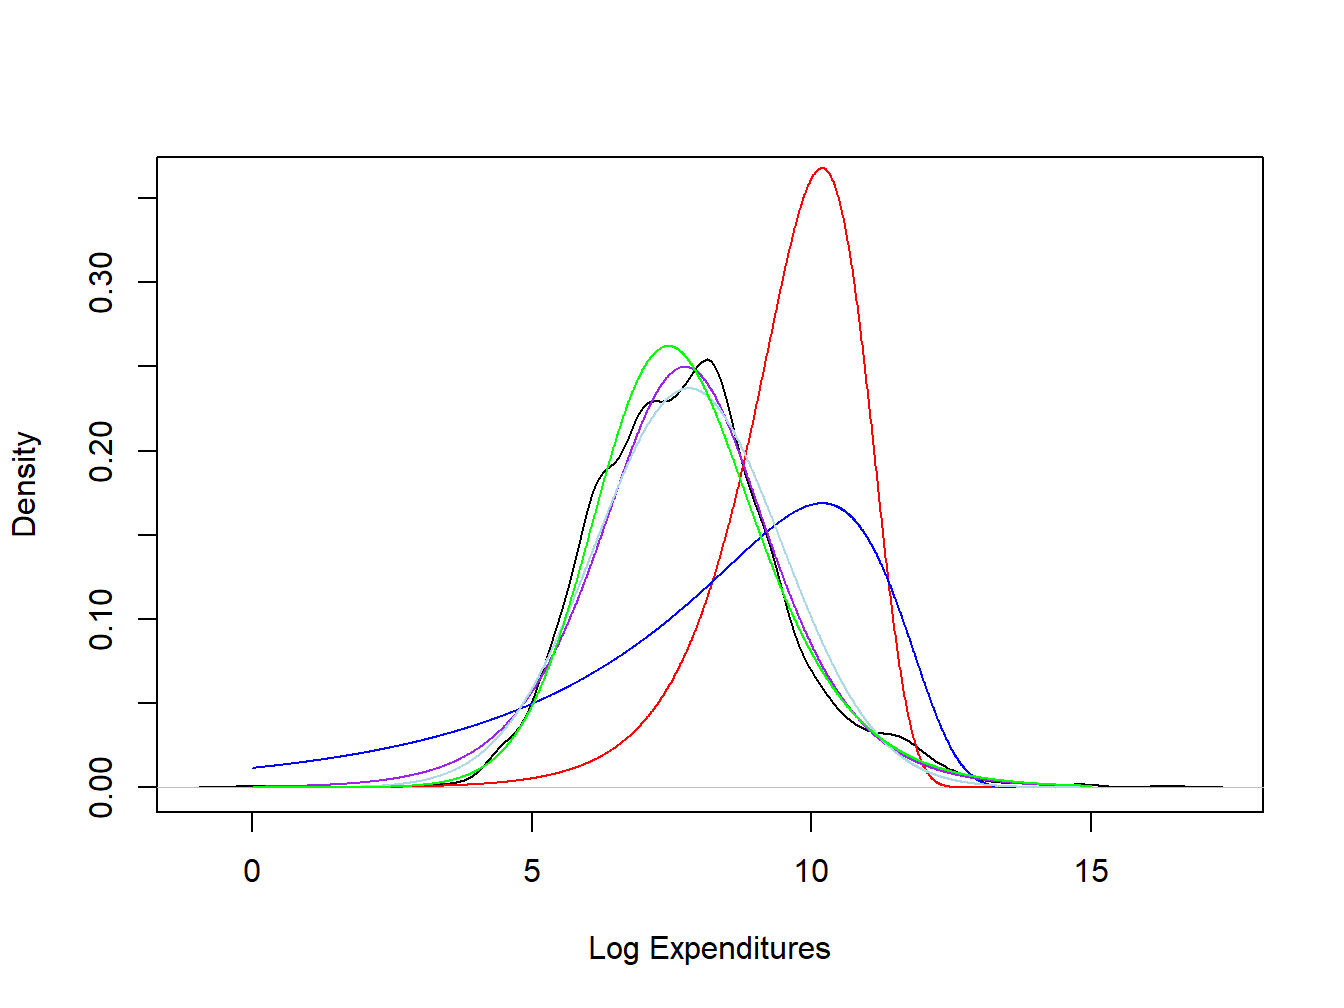
\includegraphics[width=0.8\linewidth]{LossDataAnalytics_files/figure-latex/FitClaimDistn-1} 

}

\caption{Fitted Claims Distribution}\label{fig:FitClaimDistn}
\end{figure}

R Code for Fitted Claims Distributions

\hypertarget{display.FitClaimDistn.2}{}
\begin{verbatim}
# R Code to fit several claims distributions
ClaimLev <- read.csv("Data/CLAIMLEVEL.csv", header=TRUE); nrow(ClaimLev)
ClaimData<-subset(ClaimLev,Year==2010); 
#Use "VGAM" library for estimation of parameters 
library(VGAM)
fit.LN <- vglm(Claim ~ 1, family=lognormal, data = ClaimData)
fit.gamma <- vglm(Claim ~ 1, family=gamma2, data = ClaimData)
  theta.gamma<-exp(coef(fit.gamma)[1])/exp(coef(fit.gamma)[2]) 
  alpha.gamma<-exp(coef(fit.gamma)[2])
fit.exp <- vglm(Claim ~ 1, exponential, data = ClaimData)
fit.pareto <- vglm(Claim ~ 1, paretoII, loc=0, data = ClaimData)

###################################################
#  Inference assuming a GB2 Distribution - this is more complicated
# The likelihood functon of GB2 distribution (negative for optimization)
likgb2 <- function(param) {
  a1 <- param[1]
  a2 <- param[2]
  mu <- param[3]
  sigma <- param[4]
  yt <- (log(ClaimData$Claim)-mu)/sigma
  logexpyt<-ifelse(yt>23,yt,log(1+exp(yt)))
  logdens <- a1*yt - log(sigma) - log(beta(a1,a2)) - (a1+a2)*logexpyt -log(ClaimData$Claim) 
  return(-sum(logdens))
}
#  "optim" is a general purpose minimization function
gb2bop <- optim(c(1,1,0,1),likgb2,method=c("L-BFGS-B"),
                lower=c(0.01,0.01,-500,0.01),upper=c(500,500,500,500),hessian=TRUE)
###################################################
# Plotting the fit using densities (on a logarithmic scale)
plot(density(log(ClaimData$Claim)), ylim=c(0,0.36),main="", xlab="Log Expenditures")
x <- seq(0,15,by=0.01)
fexp_ex = dgamma(exp(x), scale = exp(-coef(fit.exp)), shape = 1)*exp(x)
lines(x,fexp_ex, col="red")
fgamma_ex = dgamma(exp(x), shape = alpha.gamma, scale=theta.gamma)*exp(x)
lines(x,fgamma_ex,col="blue")
fpareto_ex = dparetoII(exp(x),loc=0,shape = exp(coef(fit.pareto)[2]), scale = exp(coef(fit.pareto)[1]))*exp(x)
lines(x,fpareto_ex,col="purple")
flnorm_ex = dlnorm(exp(x), mean = coef(fit.LN)[1], sd = exp(coef(fit.LN)[2]))*exp(x)
lines(x,flnorm_ex, col="lightblue")
# density for GB II
gb2density <- function(x){
  a1 <- gb2bop$par[1]
  a2 <- gb2bop$par[2]
  mu <- gb2bop$par[3]
  sigma <- gb2bop$par[4]
  xt <- (log(x)-mu)/sigma
  logexpxt<-ifelse(xt>23,yt,log(1+exp(xt)))
  logdens <- a1*xt - log(sigma) - log(beta(a1,a2)) - (a1+a2)*logexpxt -log(x) 
  exp(logdens)
}
fGB2_ex = gb2density(exp(x))*exp(x)
lines(x,fGB2_ex, col="green")
\end{verbatim}

\bibliography{Bibliography/packages,Bibliography/LDAReference}


\end{document}
